\chapter{Graphs}
\label{sec:graphs}


\section{Fire Weather Index variables}
FFMC: Time lag is 2/3 day
DMC: Time Lag is 12 days. DMC represents the moisture content of loosely compacted, decomposing organic matter weighing about 5 kg/m2 when dry \cite{wikifire}
DC:Time lag is 52 days \cite{AICC} dá indicação do teor de humidade nas camadas
profundas (10 a 20 cm), estimando indiretamente a intensidade dos fogos devido à secura dos
combustíveis.

\section{Sample Description}

Dia 21 de Junho As 12 horas
2022:
FWI:21.95067024230957
Drought Code (DC):  418.90625
Duff Moisture Code (DMC):  160.0711212158203
Fine Fuel Moisture Code (FFMC):  86.57350158691406

2015:
35.98046875
Drought Code (DC):  380.162109375
Duff Moisture Code (DMC):  72.5761489868164
Fine Fuel Moisture Code (FFMC):  95.732421875

2019:
22.05933380126953
Drought Code (DC):  384.6829833984375
Duff Moisture Code (DMC):  97.203125
Fine Fuel Moisture Code (FFMC):  87.82327270507812

\section{Simulated FWI variables}
Este local não teve incêndio
\begin{figure}[h]
\caption{Comparison of FWI calculated values and Copernicus}
    \centering
    \begin{subfigure}{0.49\textwidth}
        \centering
        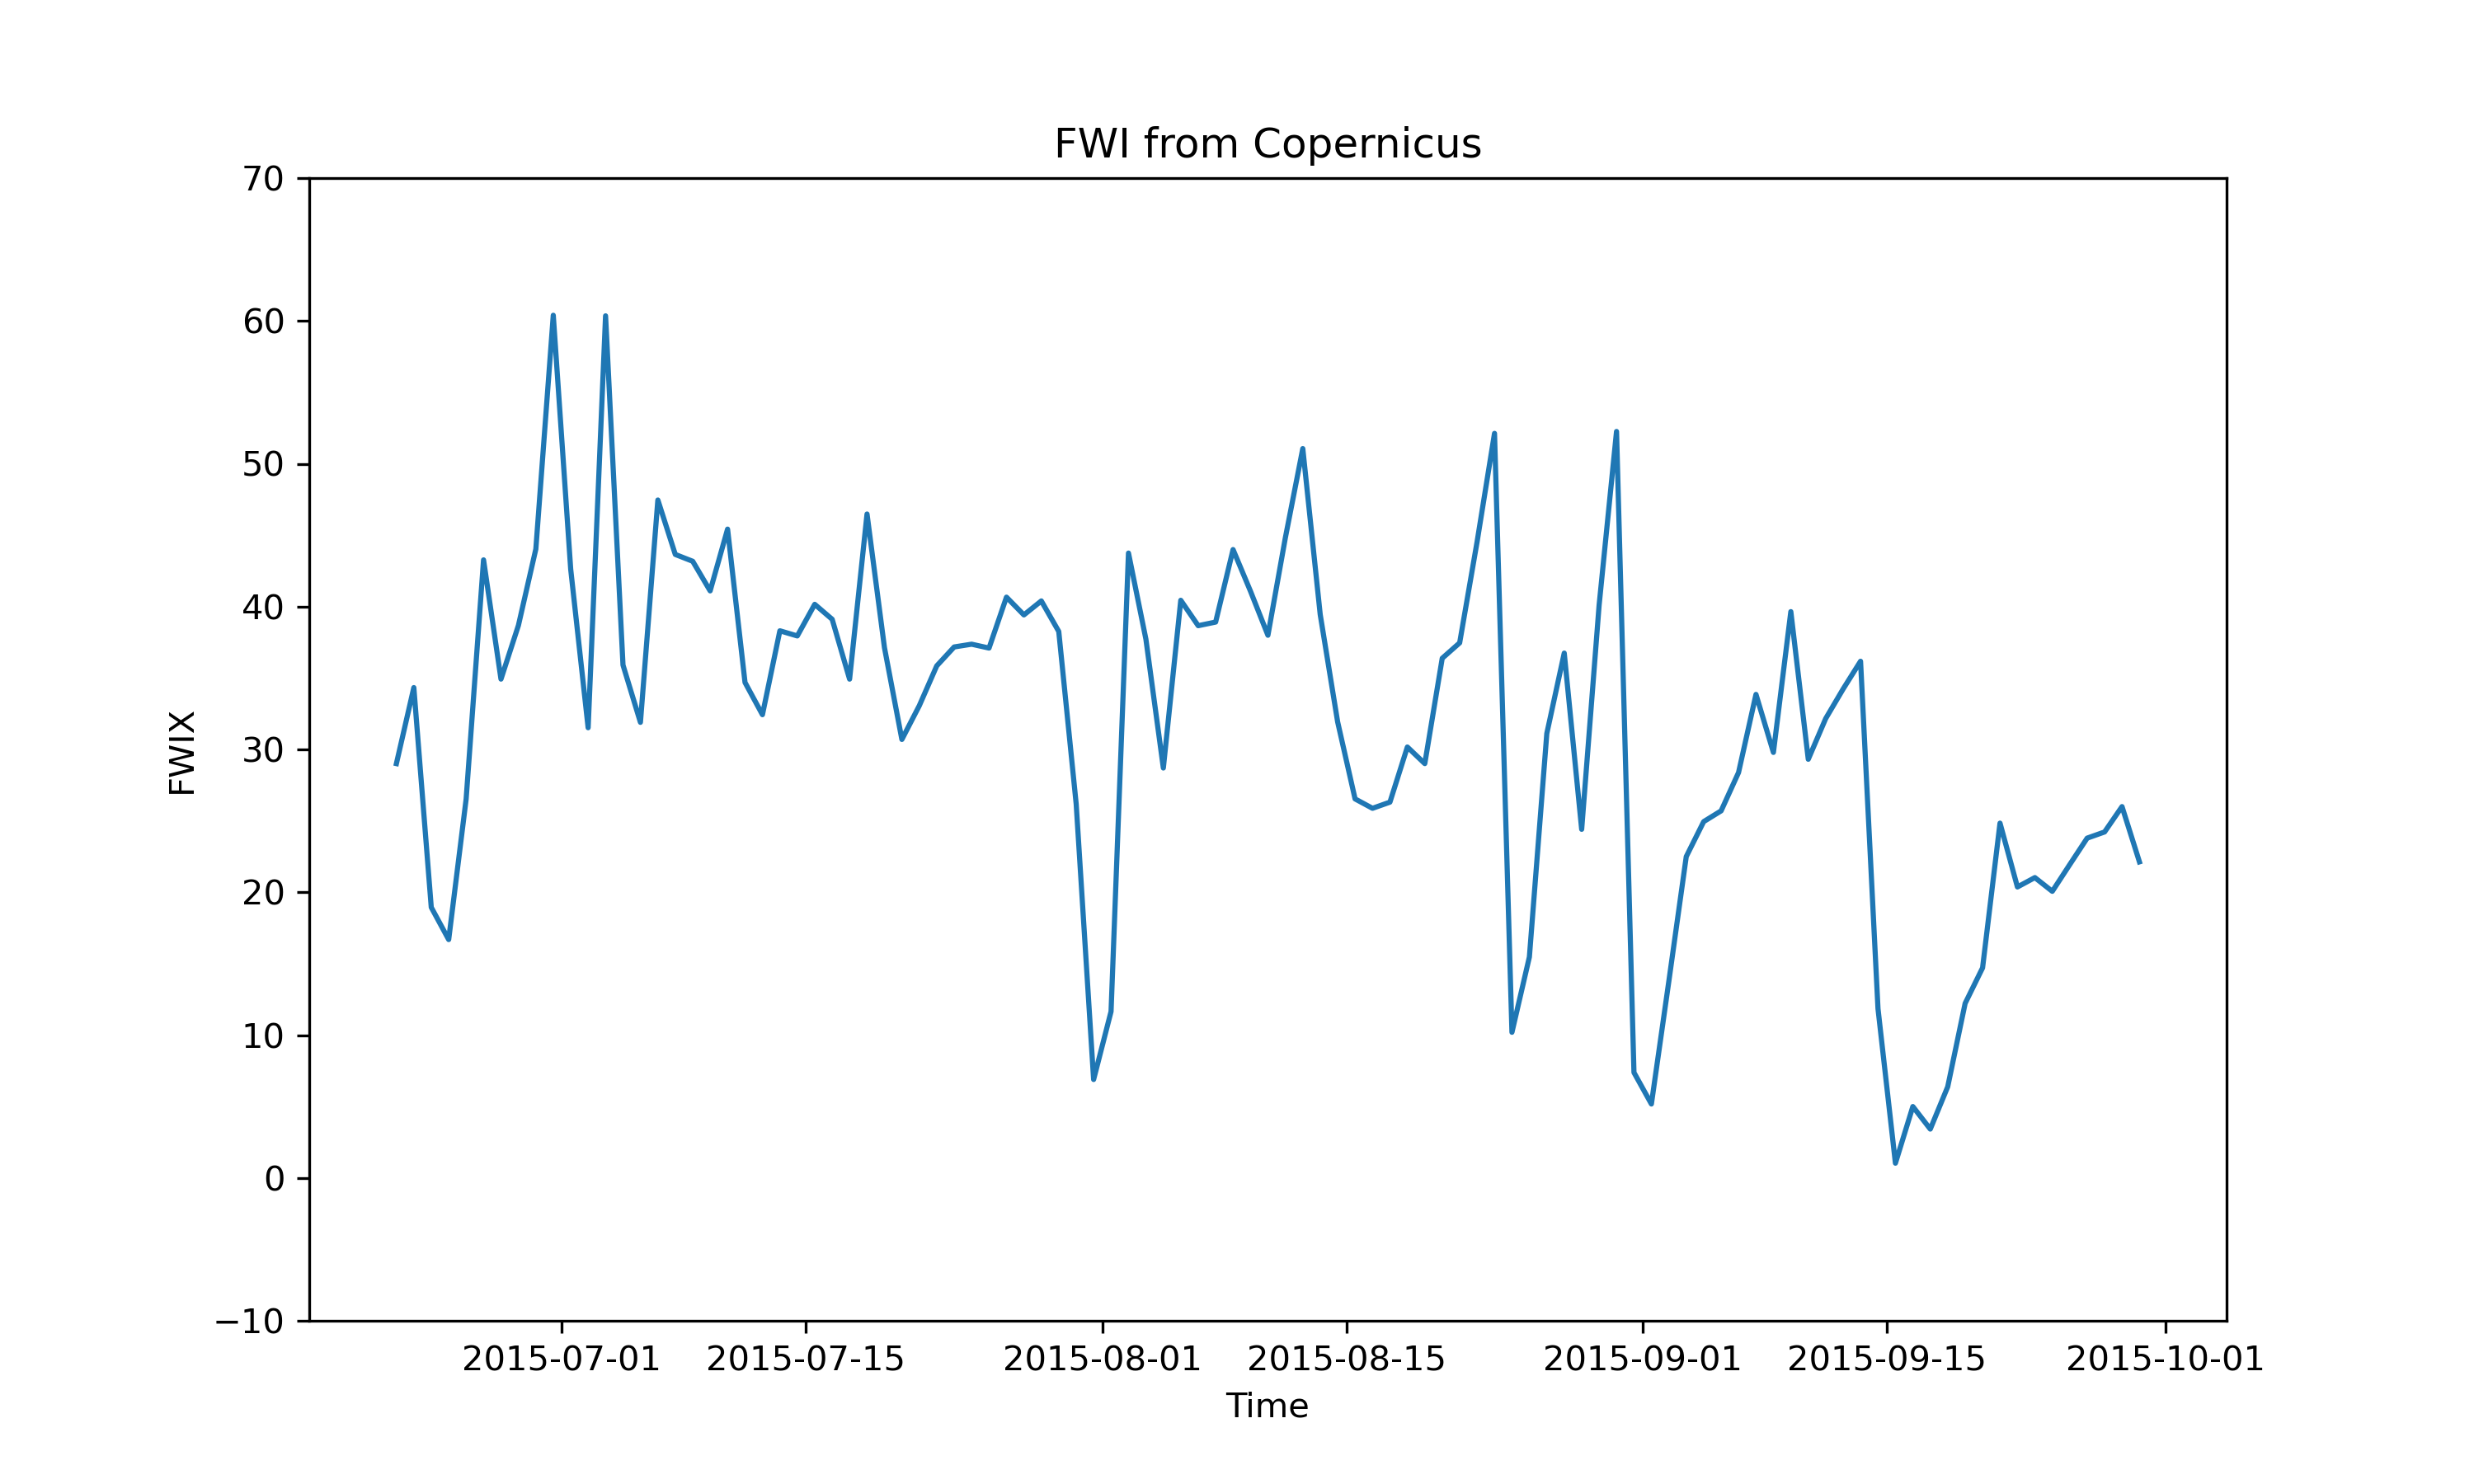
\includegraphics[width=\textwidth]{graphs/2015MesmoSitio/2015CopernicusFWI12.png}
        \caption{FWI - Copernicus}
        \label{fig:fwi_copernicus_2015_semfogo}
    \end{subfigure}
    \hfill
    \begin{subfigure}{0.49\textwidth}
        \centering
        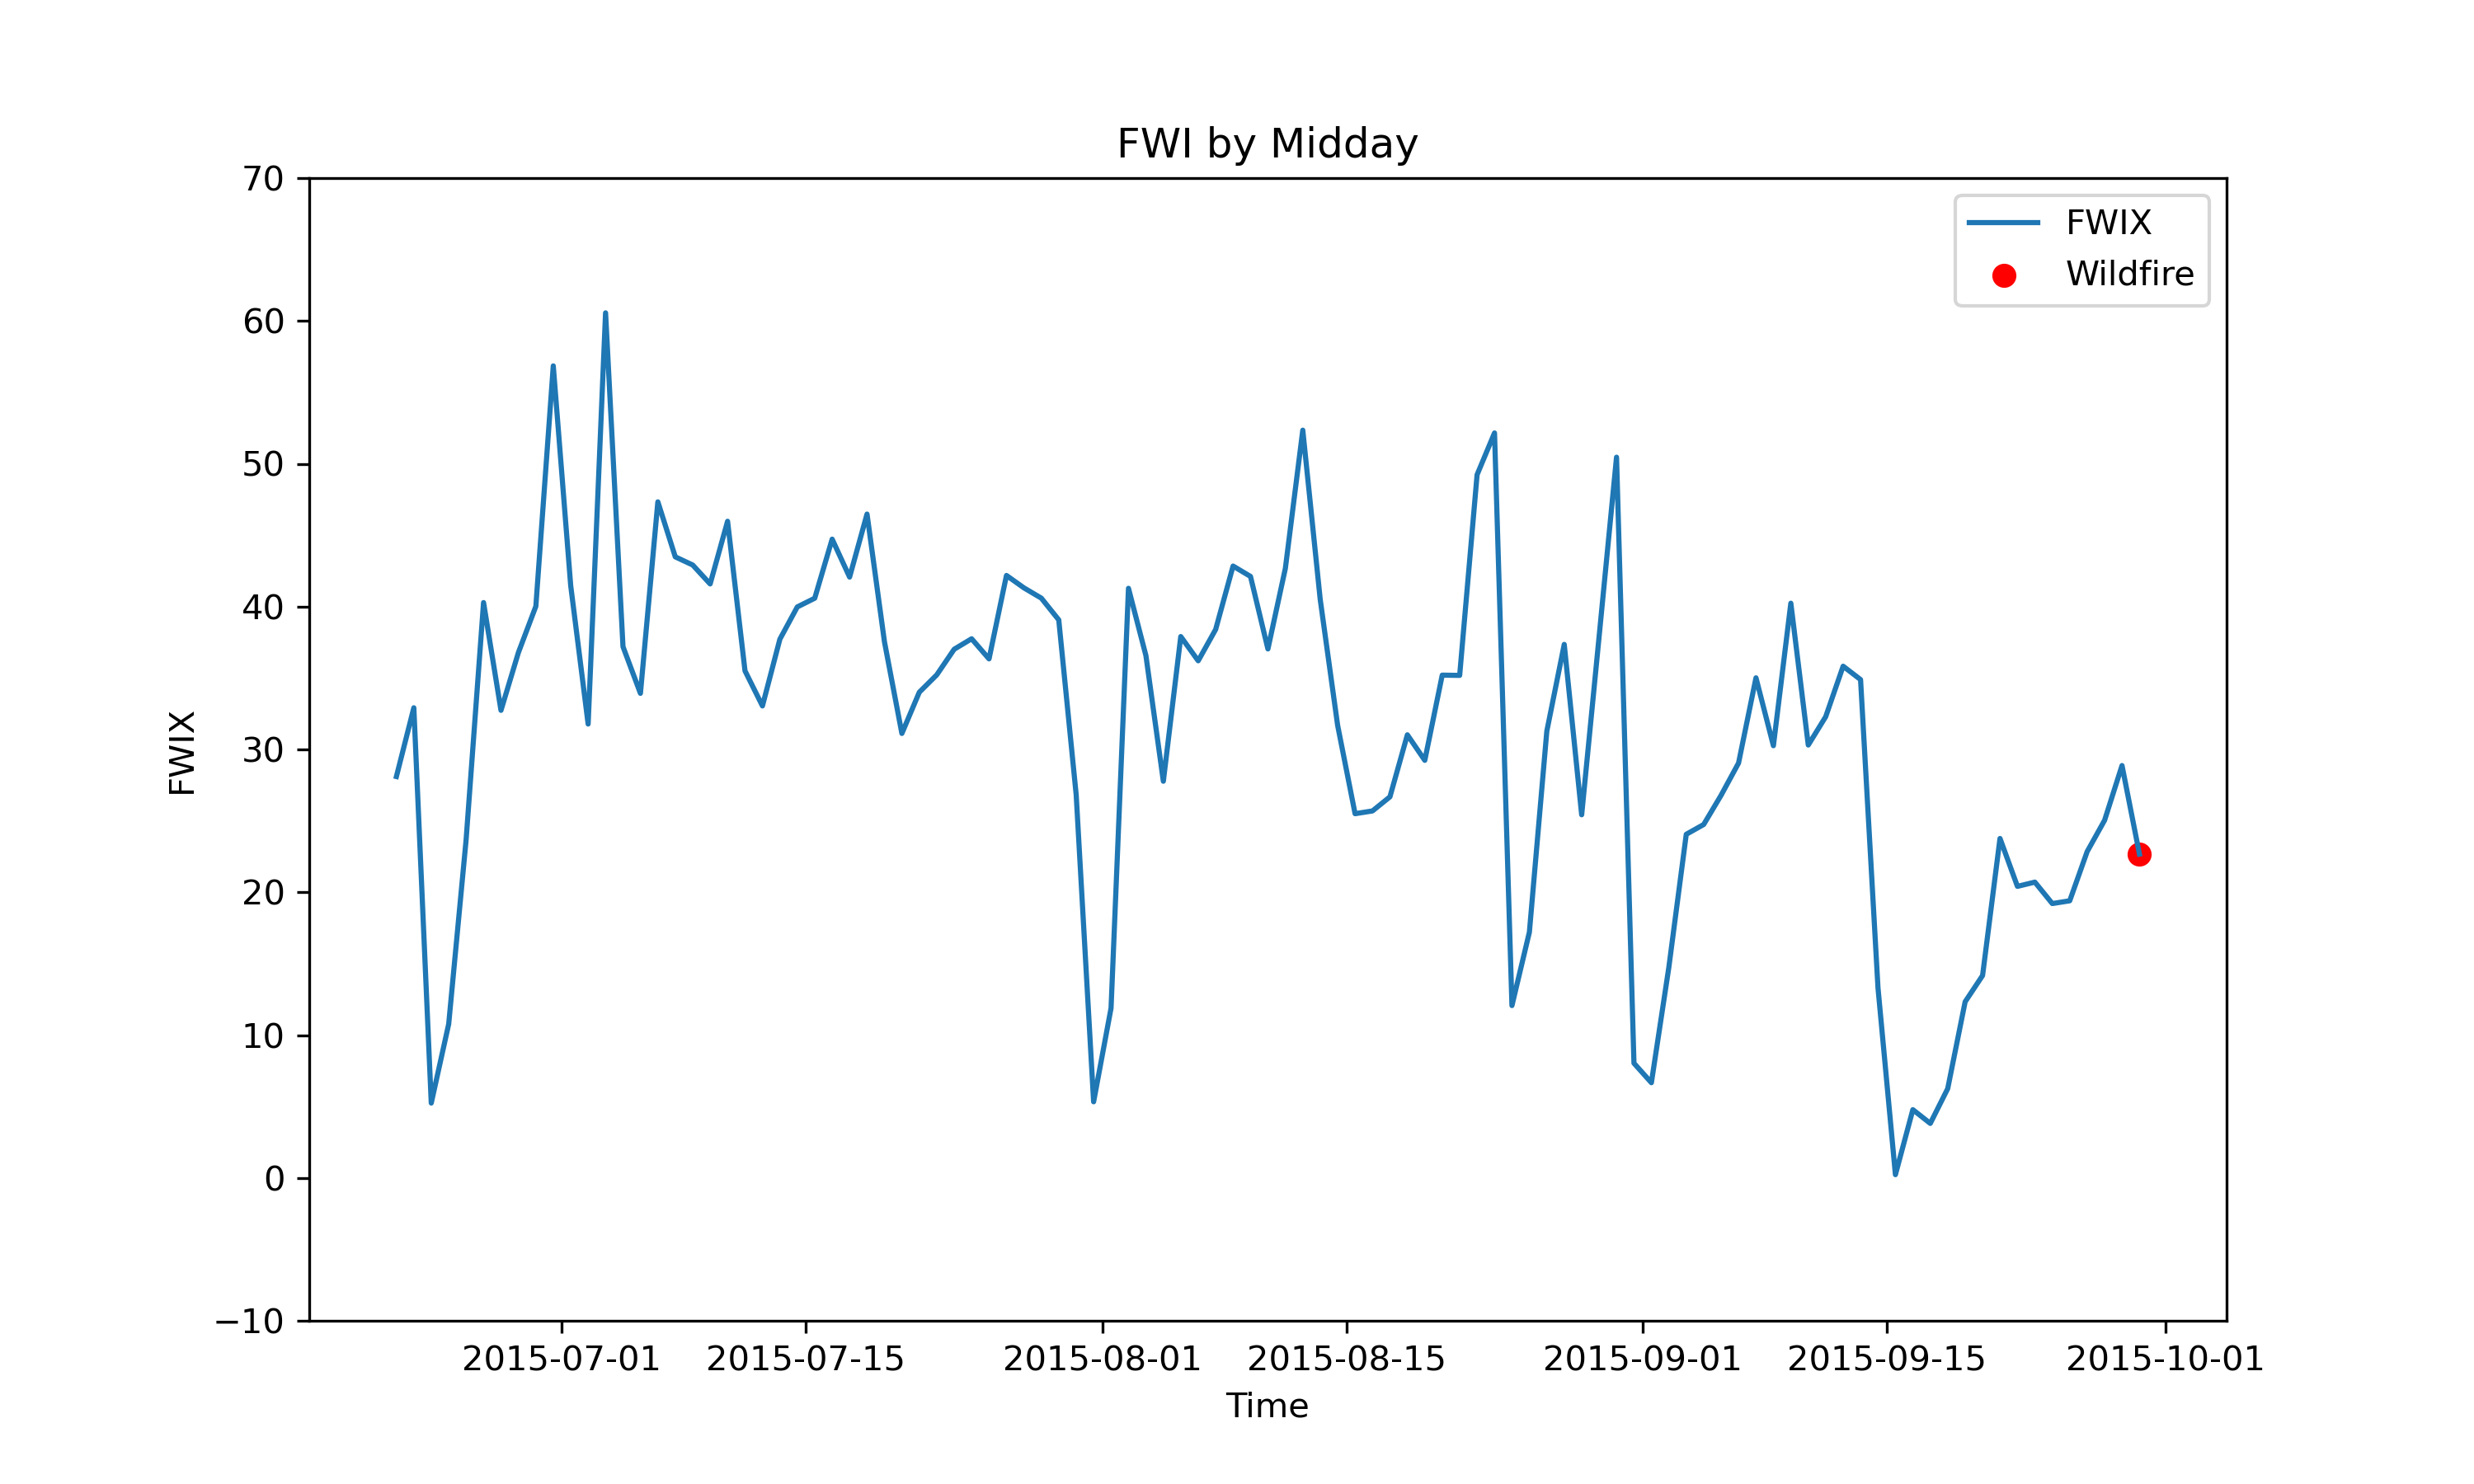
\includegraphics[width=\textwidth]{graphs/2015MesmoSitio/2015CalcFWI12.png}
        \caption{FWI - Calculated value}
        \label{fig:fwi_calculated_2015_semfogo}
    \end{subfigure}
    \label{fig:comparison_semfogo_copernicus_calculated}
\end{figure}

\begin{figure}[h]
\caption{Comparison of FFMC calculated values and Copernicus}
    \centering
    \begin{subfigure}{0.49\textwidth}
        \centering
        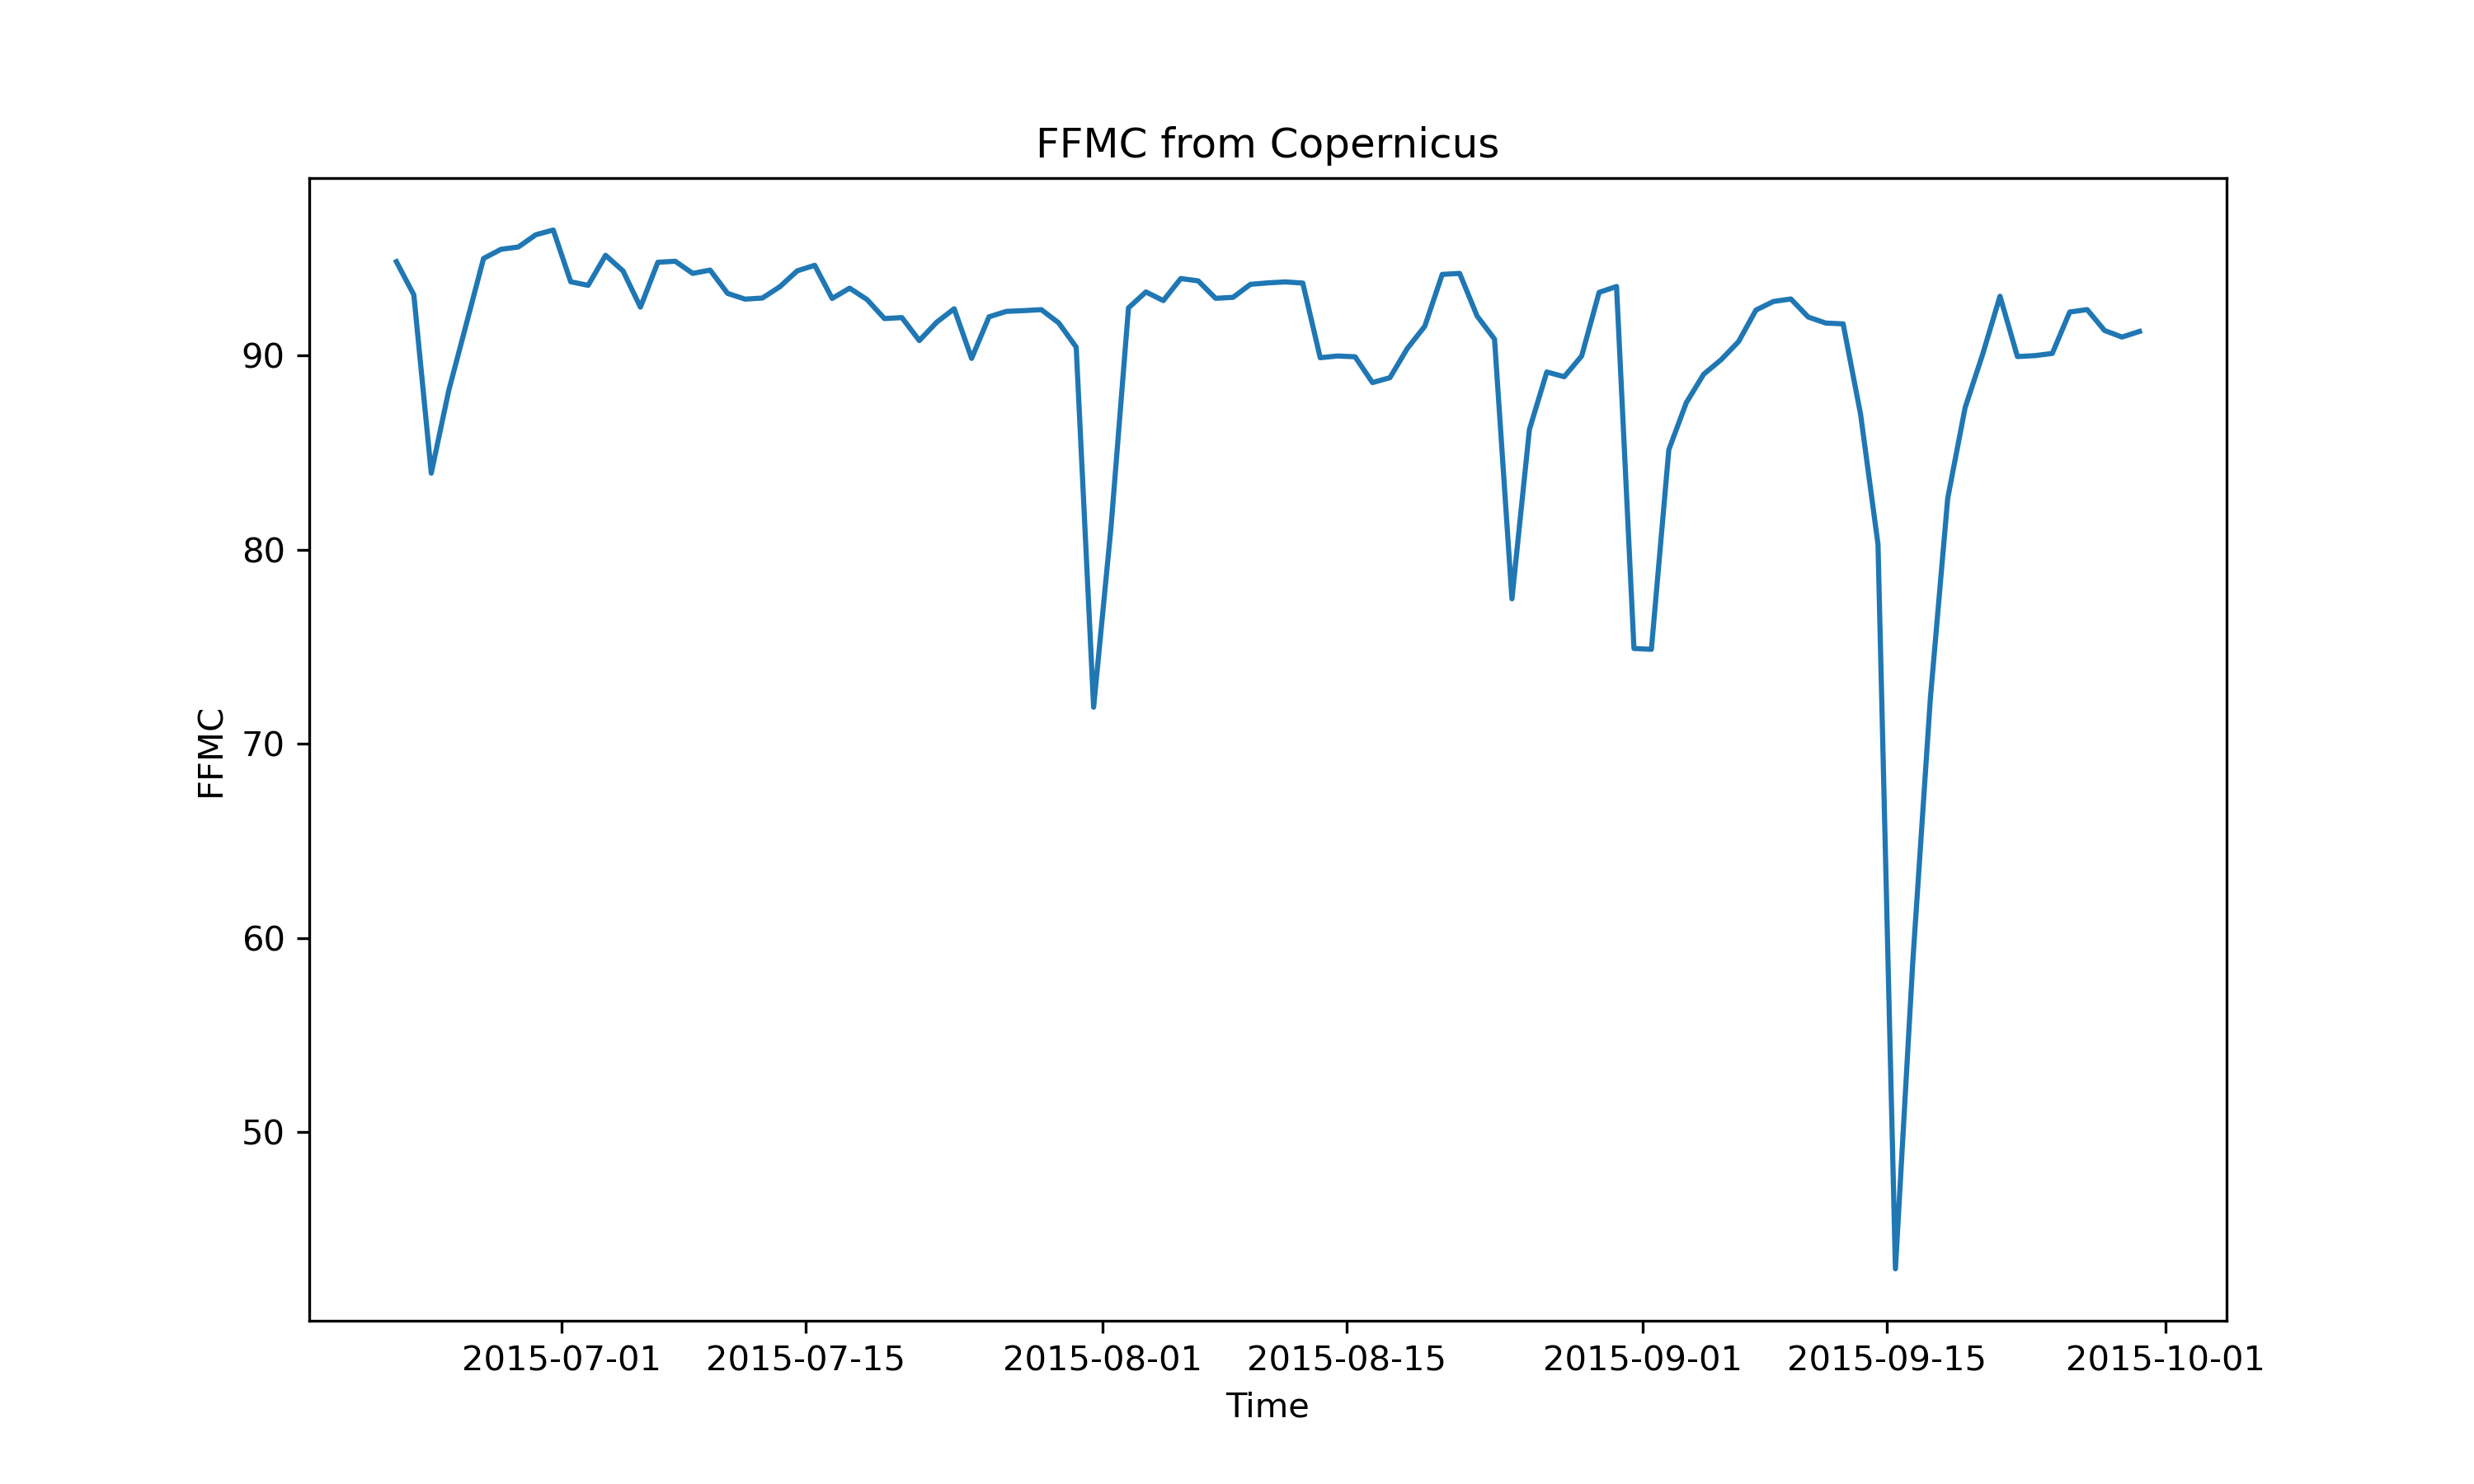
\includegraphics[width=\textwidth]{graphs/2015MesmoSitio/2015CopernicusFFMC12.png}
        \caption{FFMC - Copernicus}
        \label{fig:ffmc_copernicus_2015_semfogo}
    \end{subfigure}
    \hfill
    \begin{subfigure}{0.49\textwidth}
        \centering
        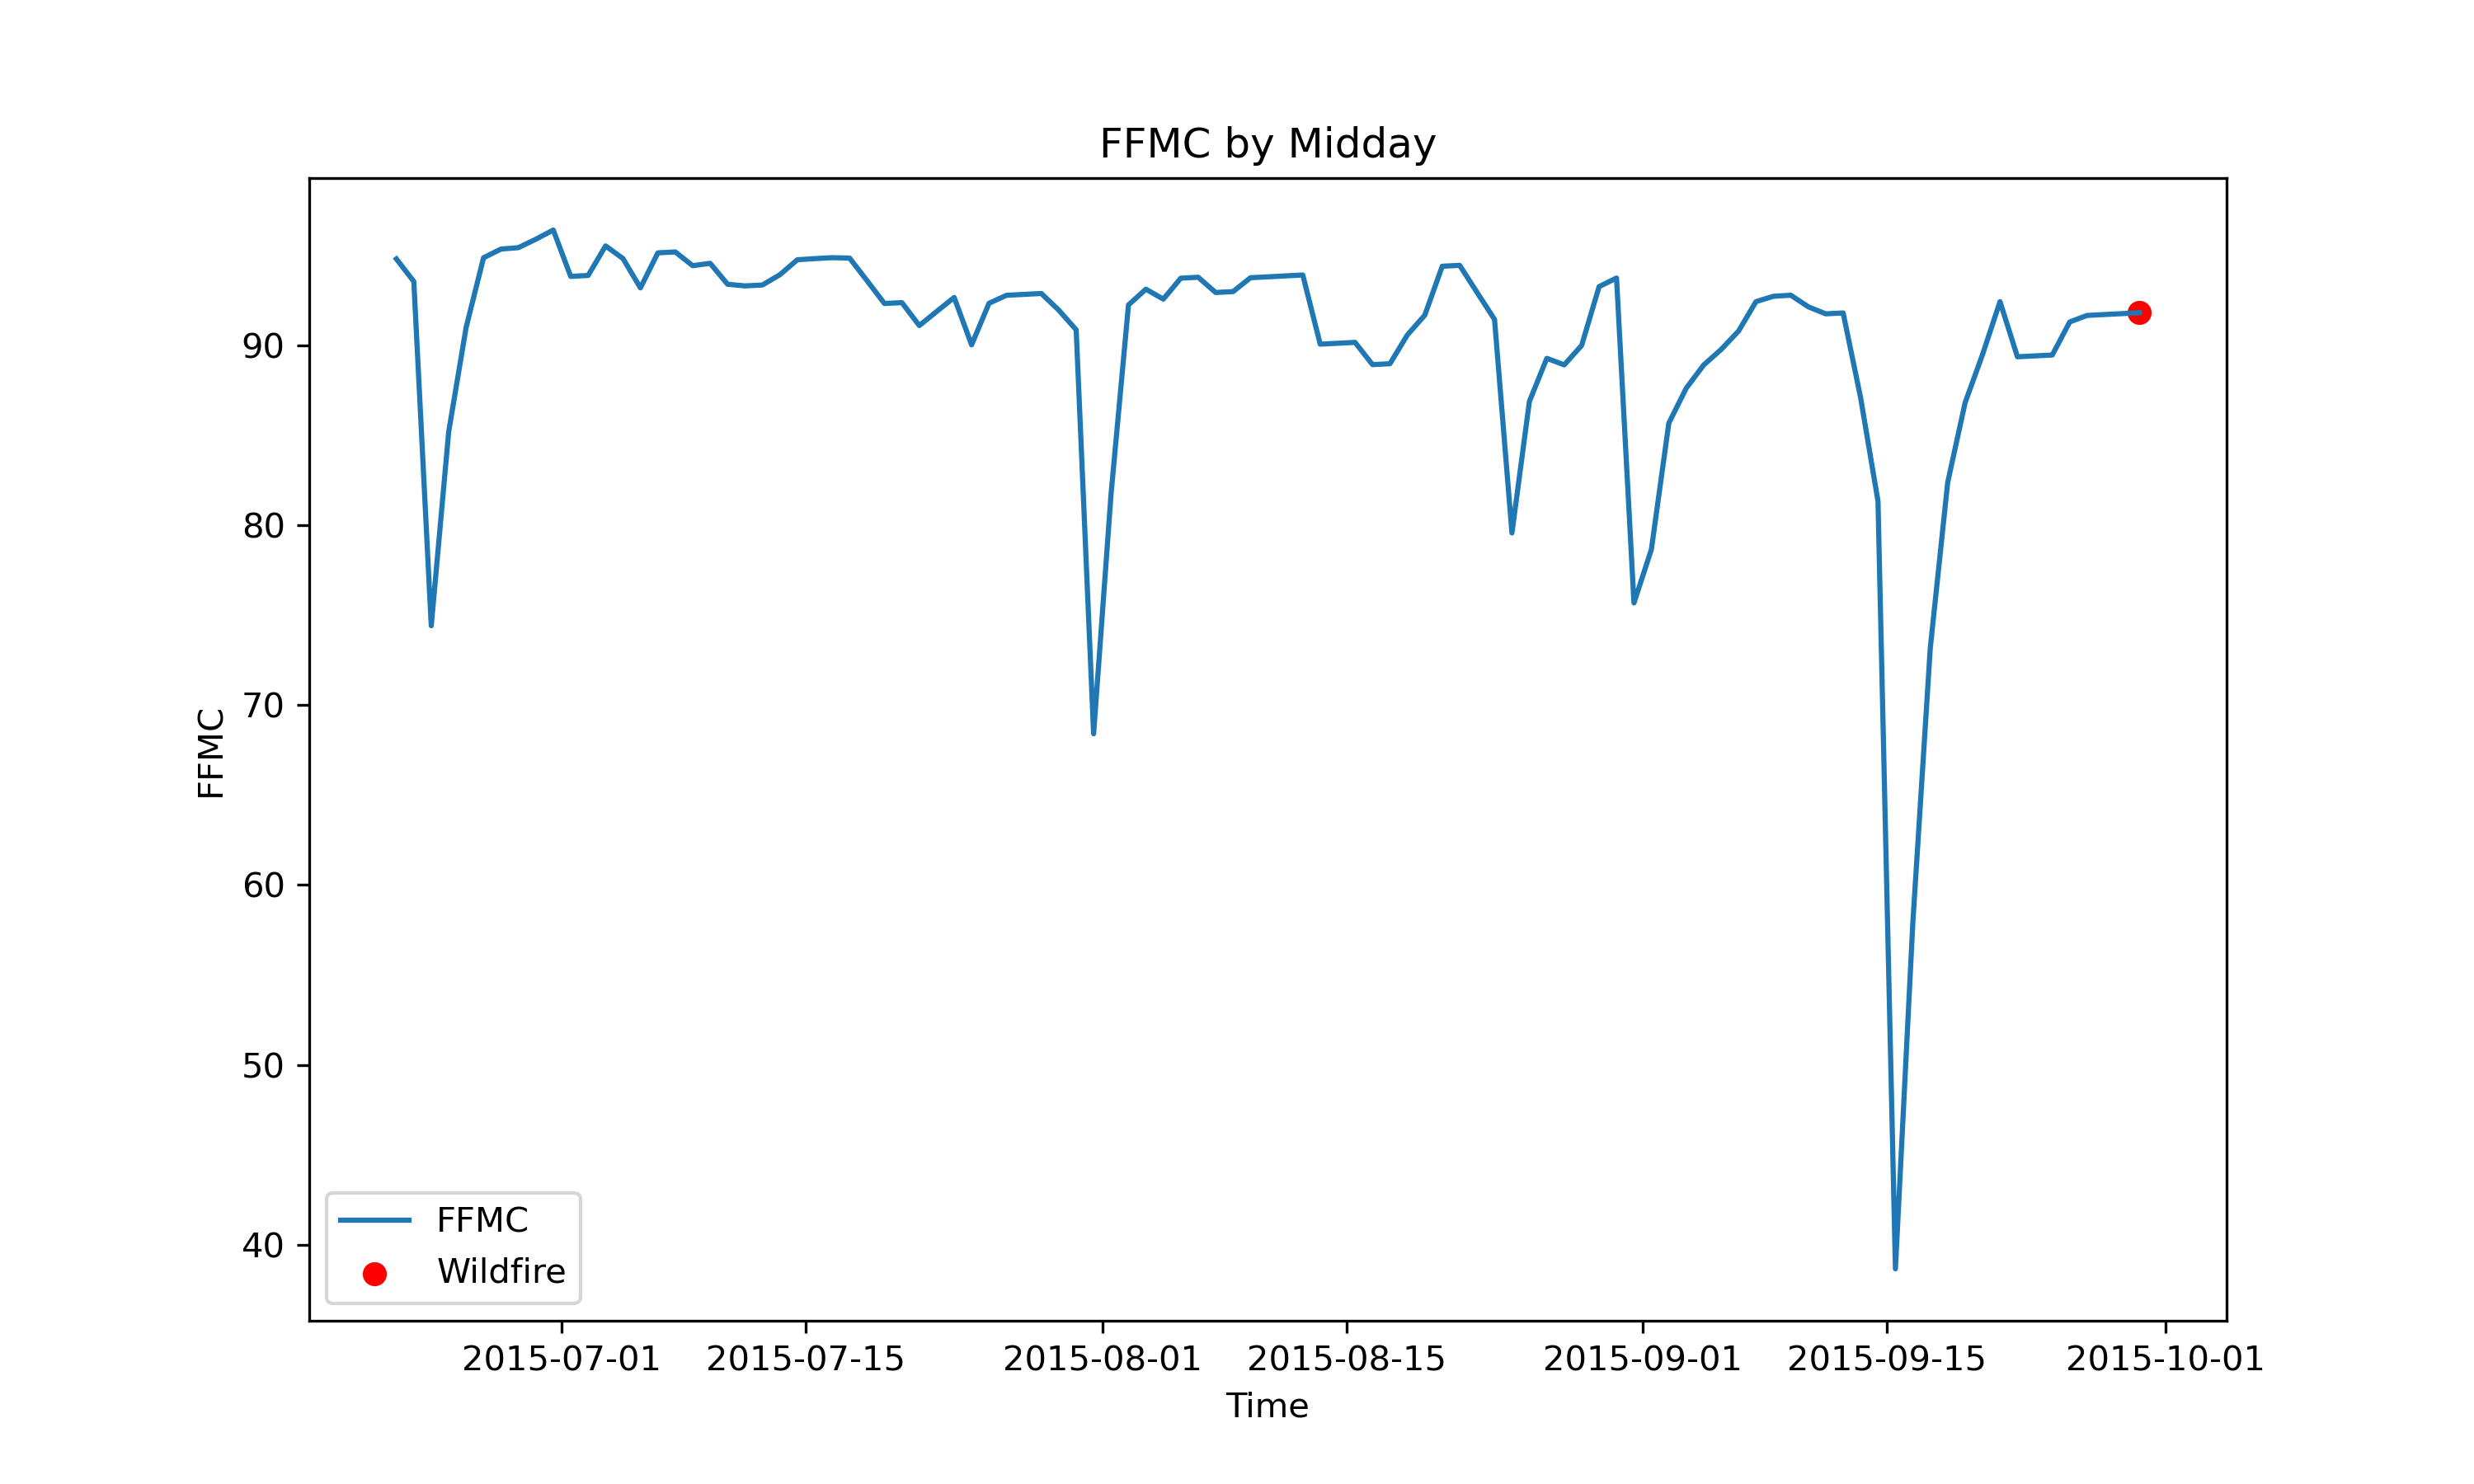
\includegraphics[width=\textwidth]{graphs/2015MesmoSitio/2015CalcFFMC12.png}
        \caption{FFMC - Calculated value}
        \label{fig:ffmc_calculated_2015_semfogo}
    \end{subfigure}
    \label{fig:comparison_ffmc_semfogo_copernicus_calculated}
\end{figure}

\begin{figure}[h]
\caption{Comparison of DMC calculated values and Copernicus}
    \centering
    \begin{subfigure}{0.49\textwidth}
        \centering
        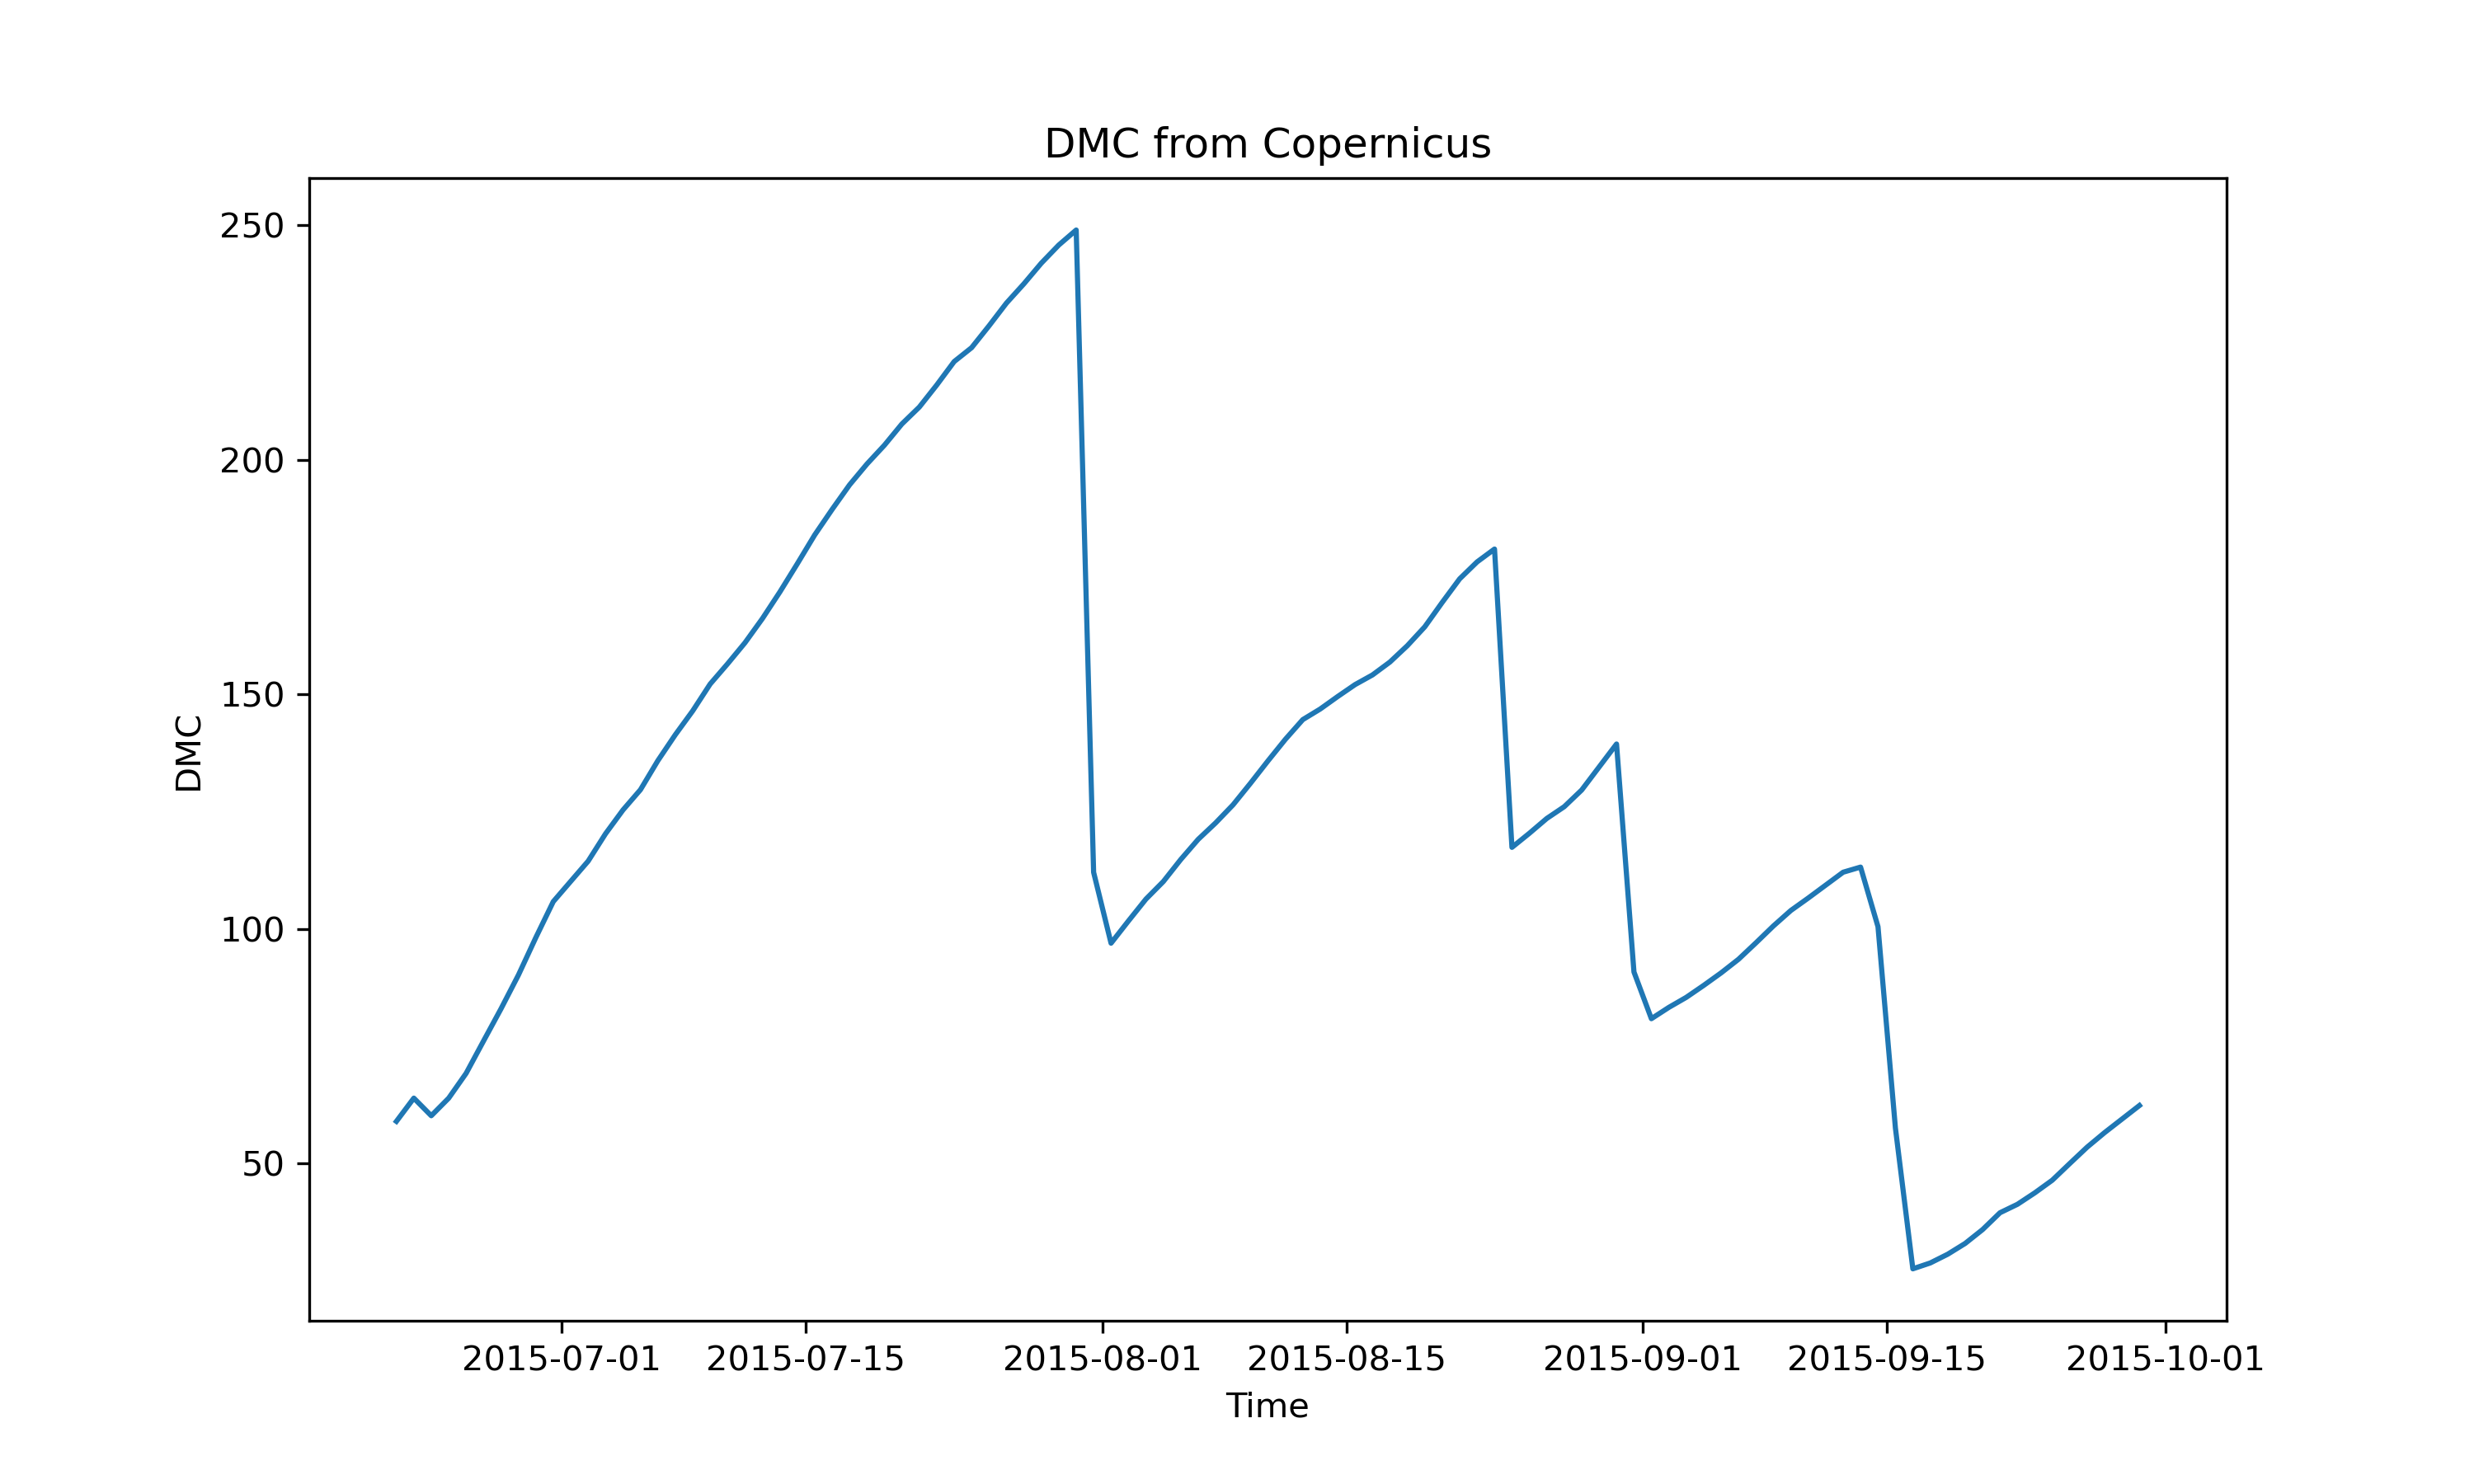
\includegraphics[width=\textwidth]{graphs/2015MesmoSitio/2015CopernicusDMC12.png}
        \caption{DMC - Copernicus}
        \label{fig:dmc_copernicus_2015_semfogo}
    \end{subfigure}
    \hfill
    \begin{subfigure}{0.49\textwidth}
        \centering
        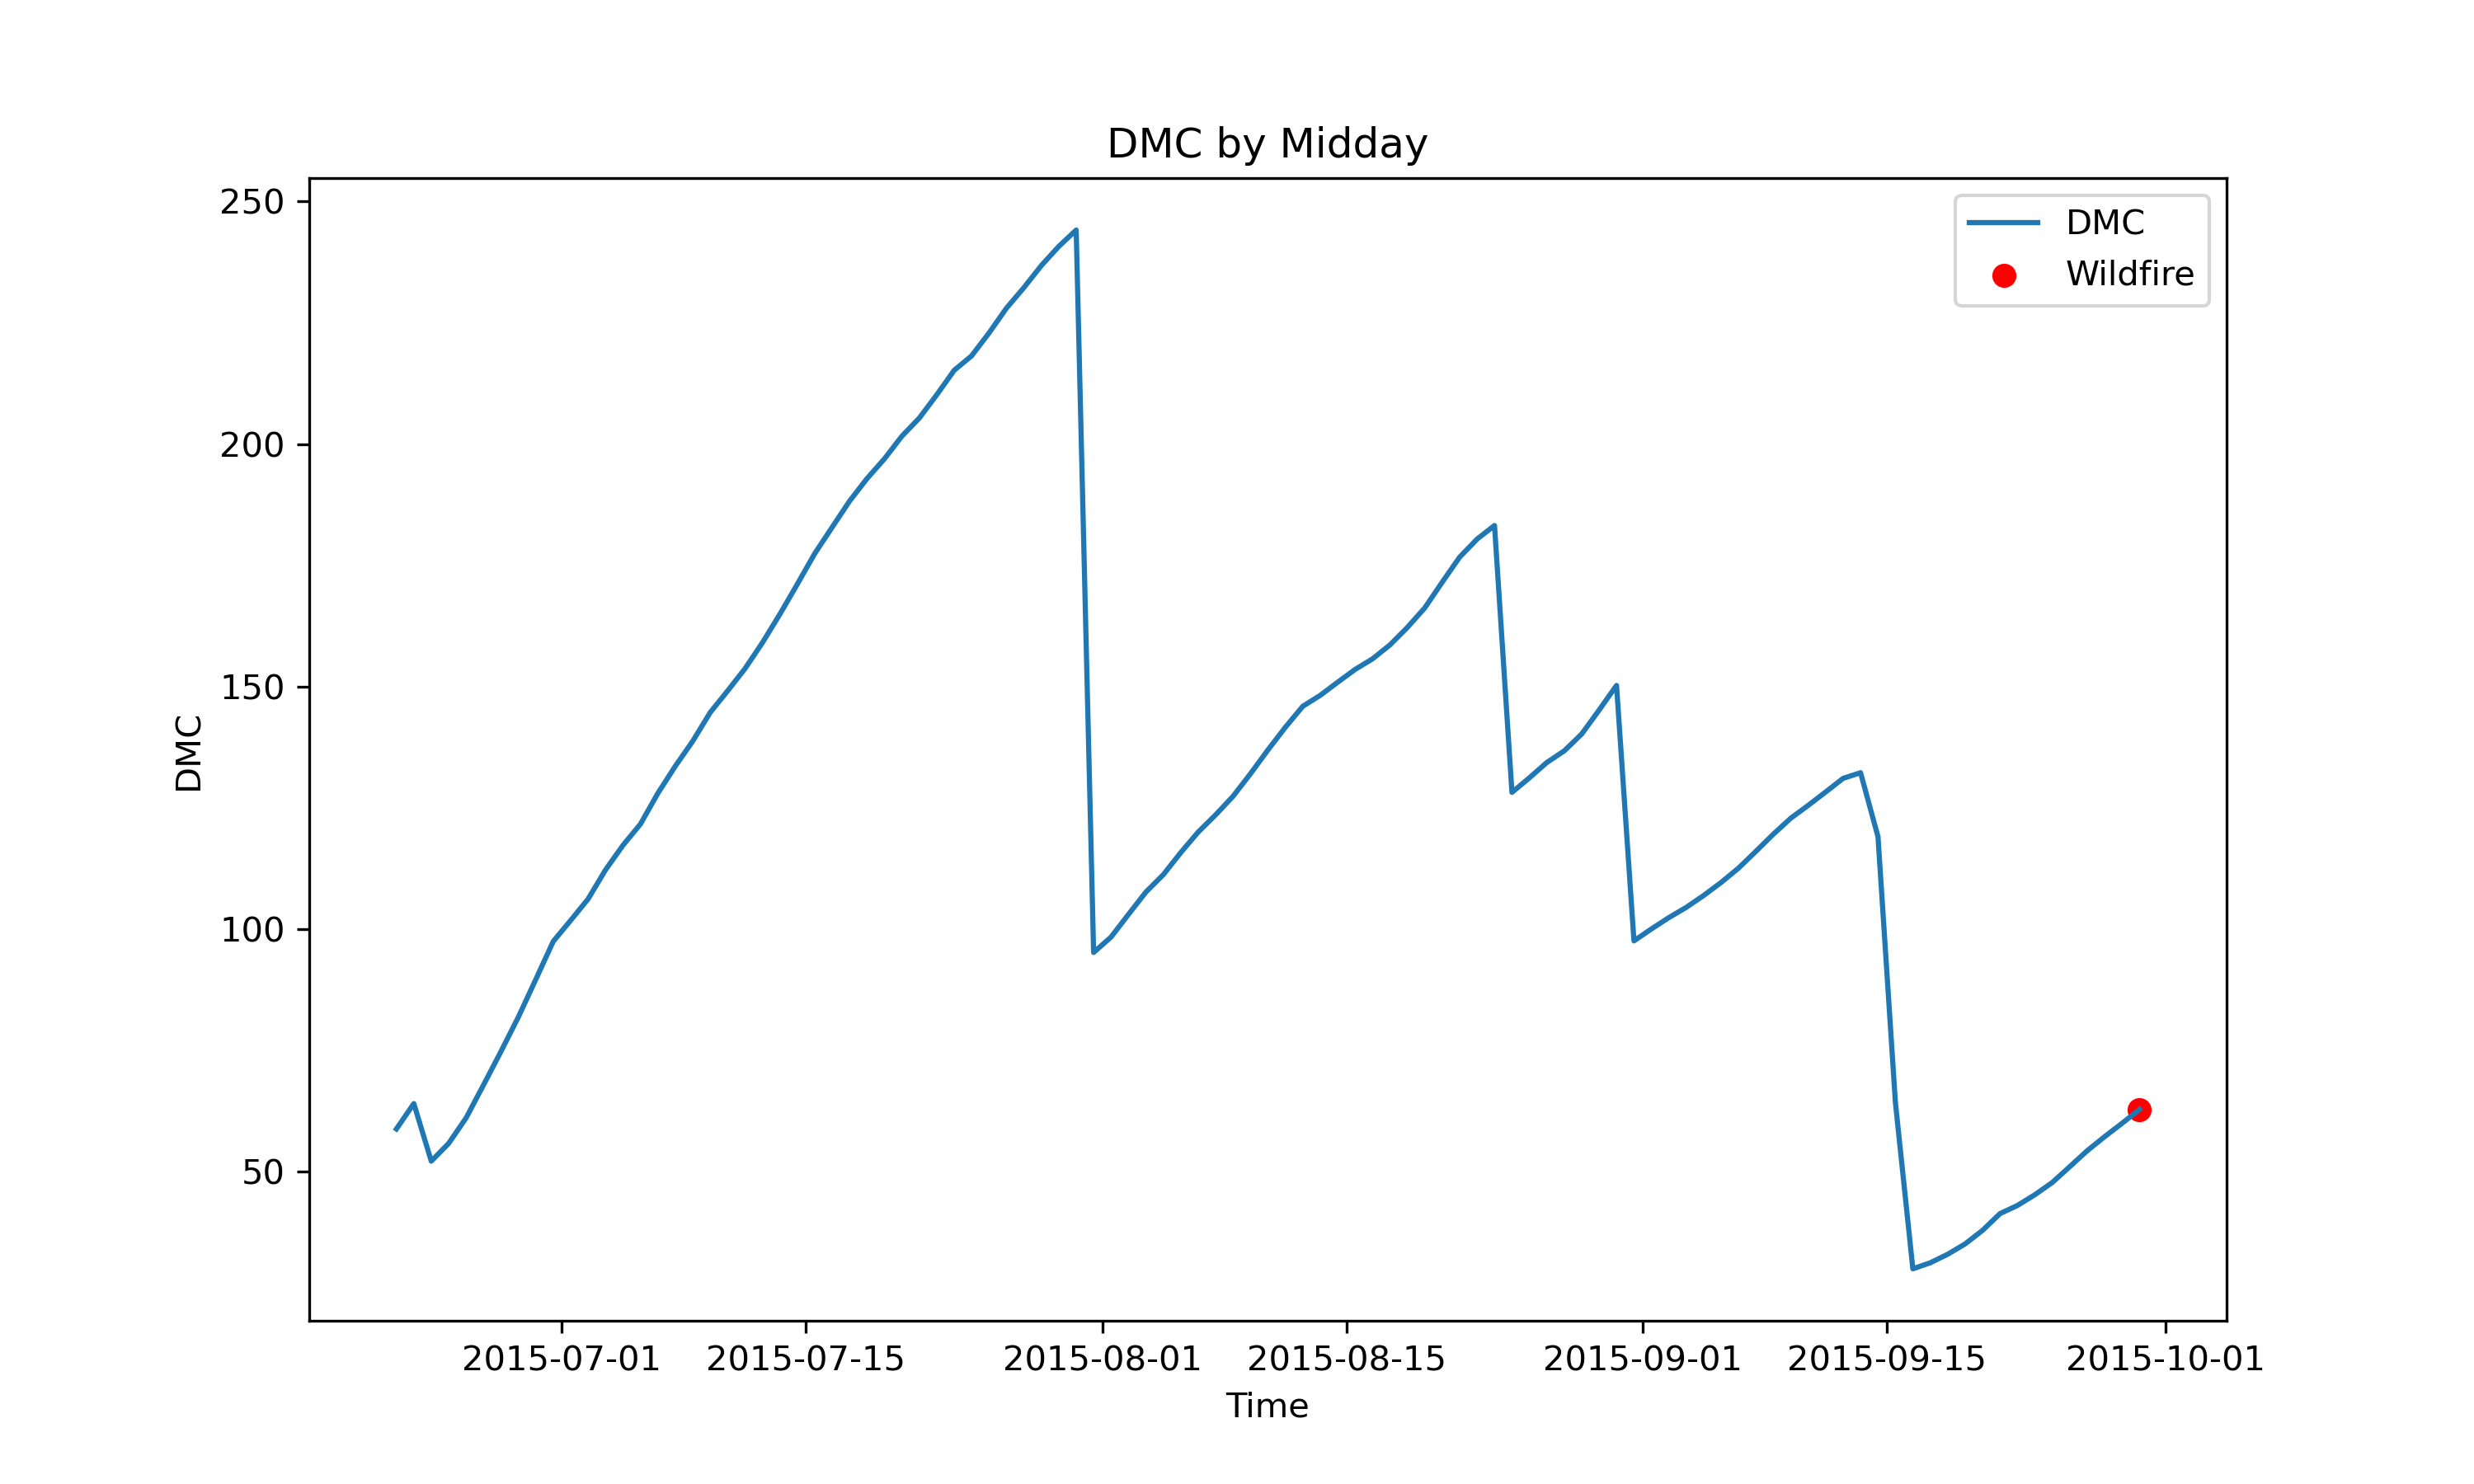
\includegraphics[width=\textwidth]{graphs/2015MesmoSitio/2015CalcDMC12.png}
        \caption{DMC - Calculated value}
        \label{fig:dmc_calculated_2015_semfogo}
    \end{subfigure}
    \label{fig:comparison_dmc_semfogo_copernicus_calculated}
\end{figure}

\begin{figure}[h]
\caption{Comparison of DC calculated values and Copernicus}
    \centering
    \begin{subfigure}{0.49\textwidth}
        \centering
        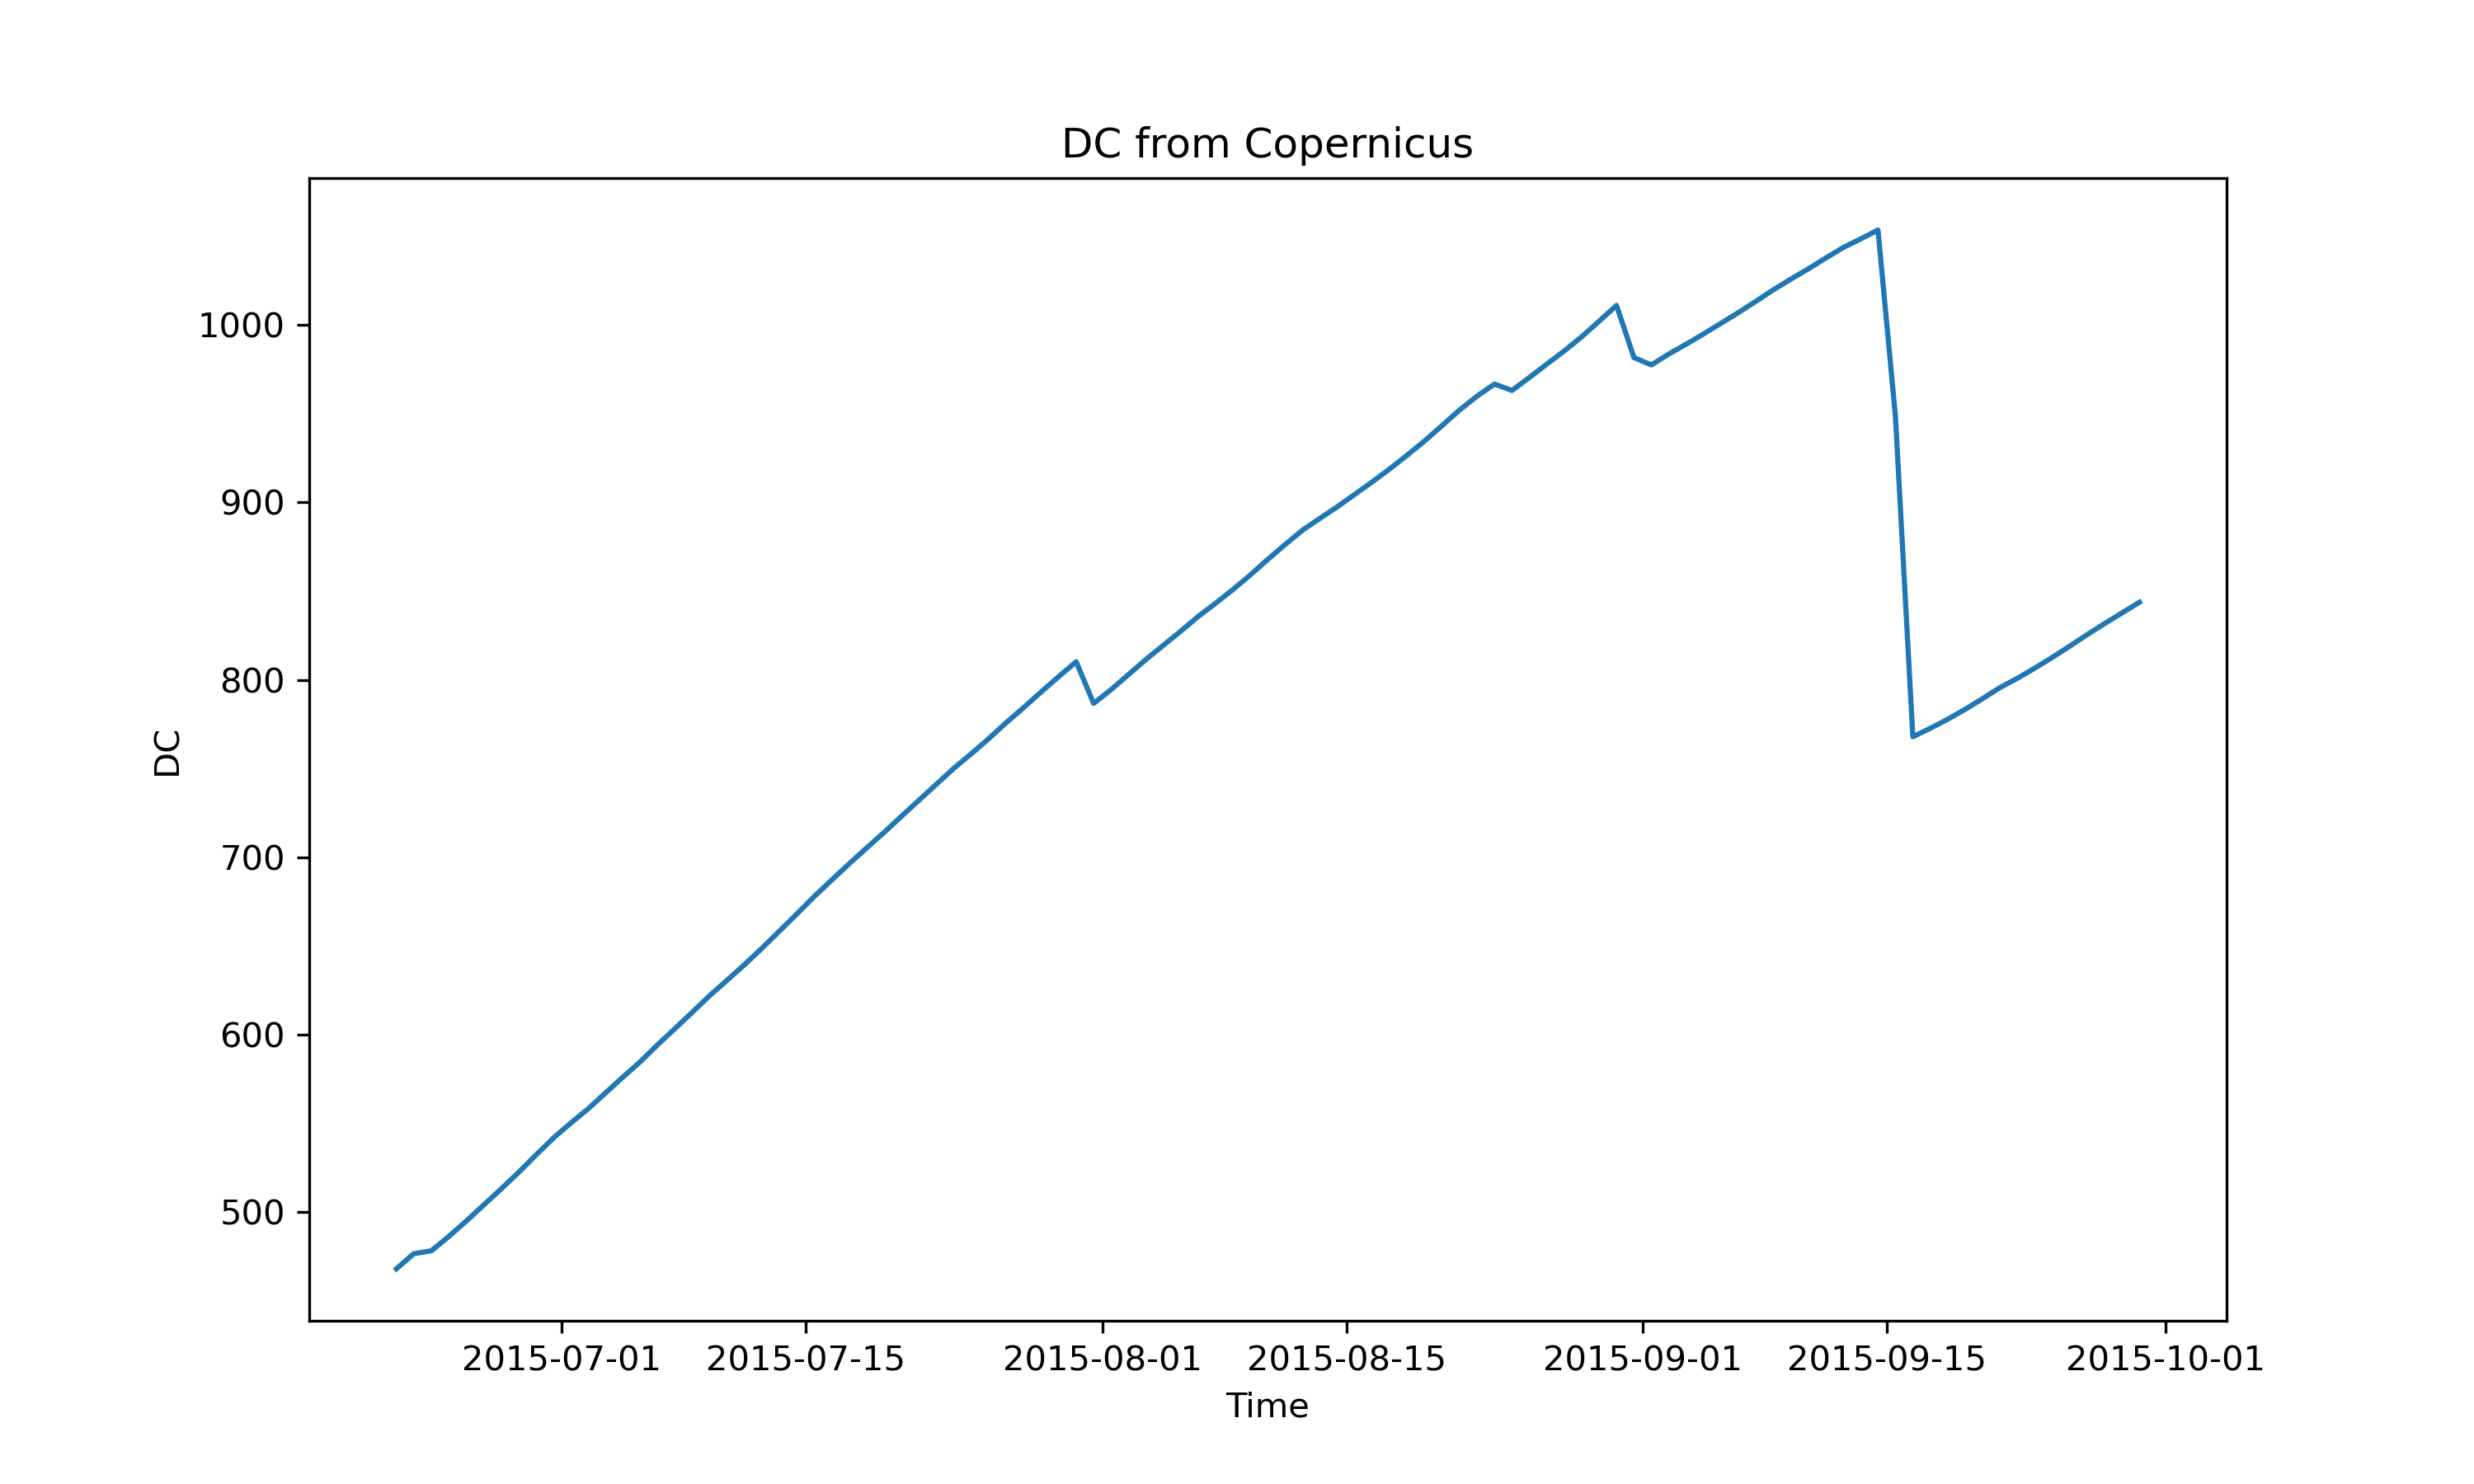
\includegraphics[width=\textwidth]{graphs/2015MesmoSitio/2015CopernicusDC12.png}
        \caption{DC - Copernicus}
        \label{fig:dc_copernicus_2015_semfogo}
    \end{subfigure}
    \hfill
    \begin{subfigure}{0.49\textwidth}
        \centering
        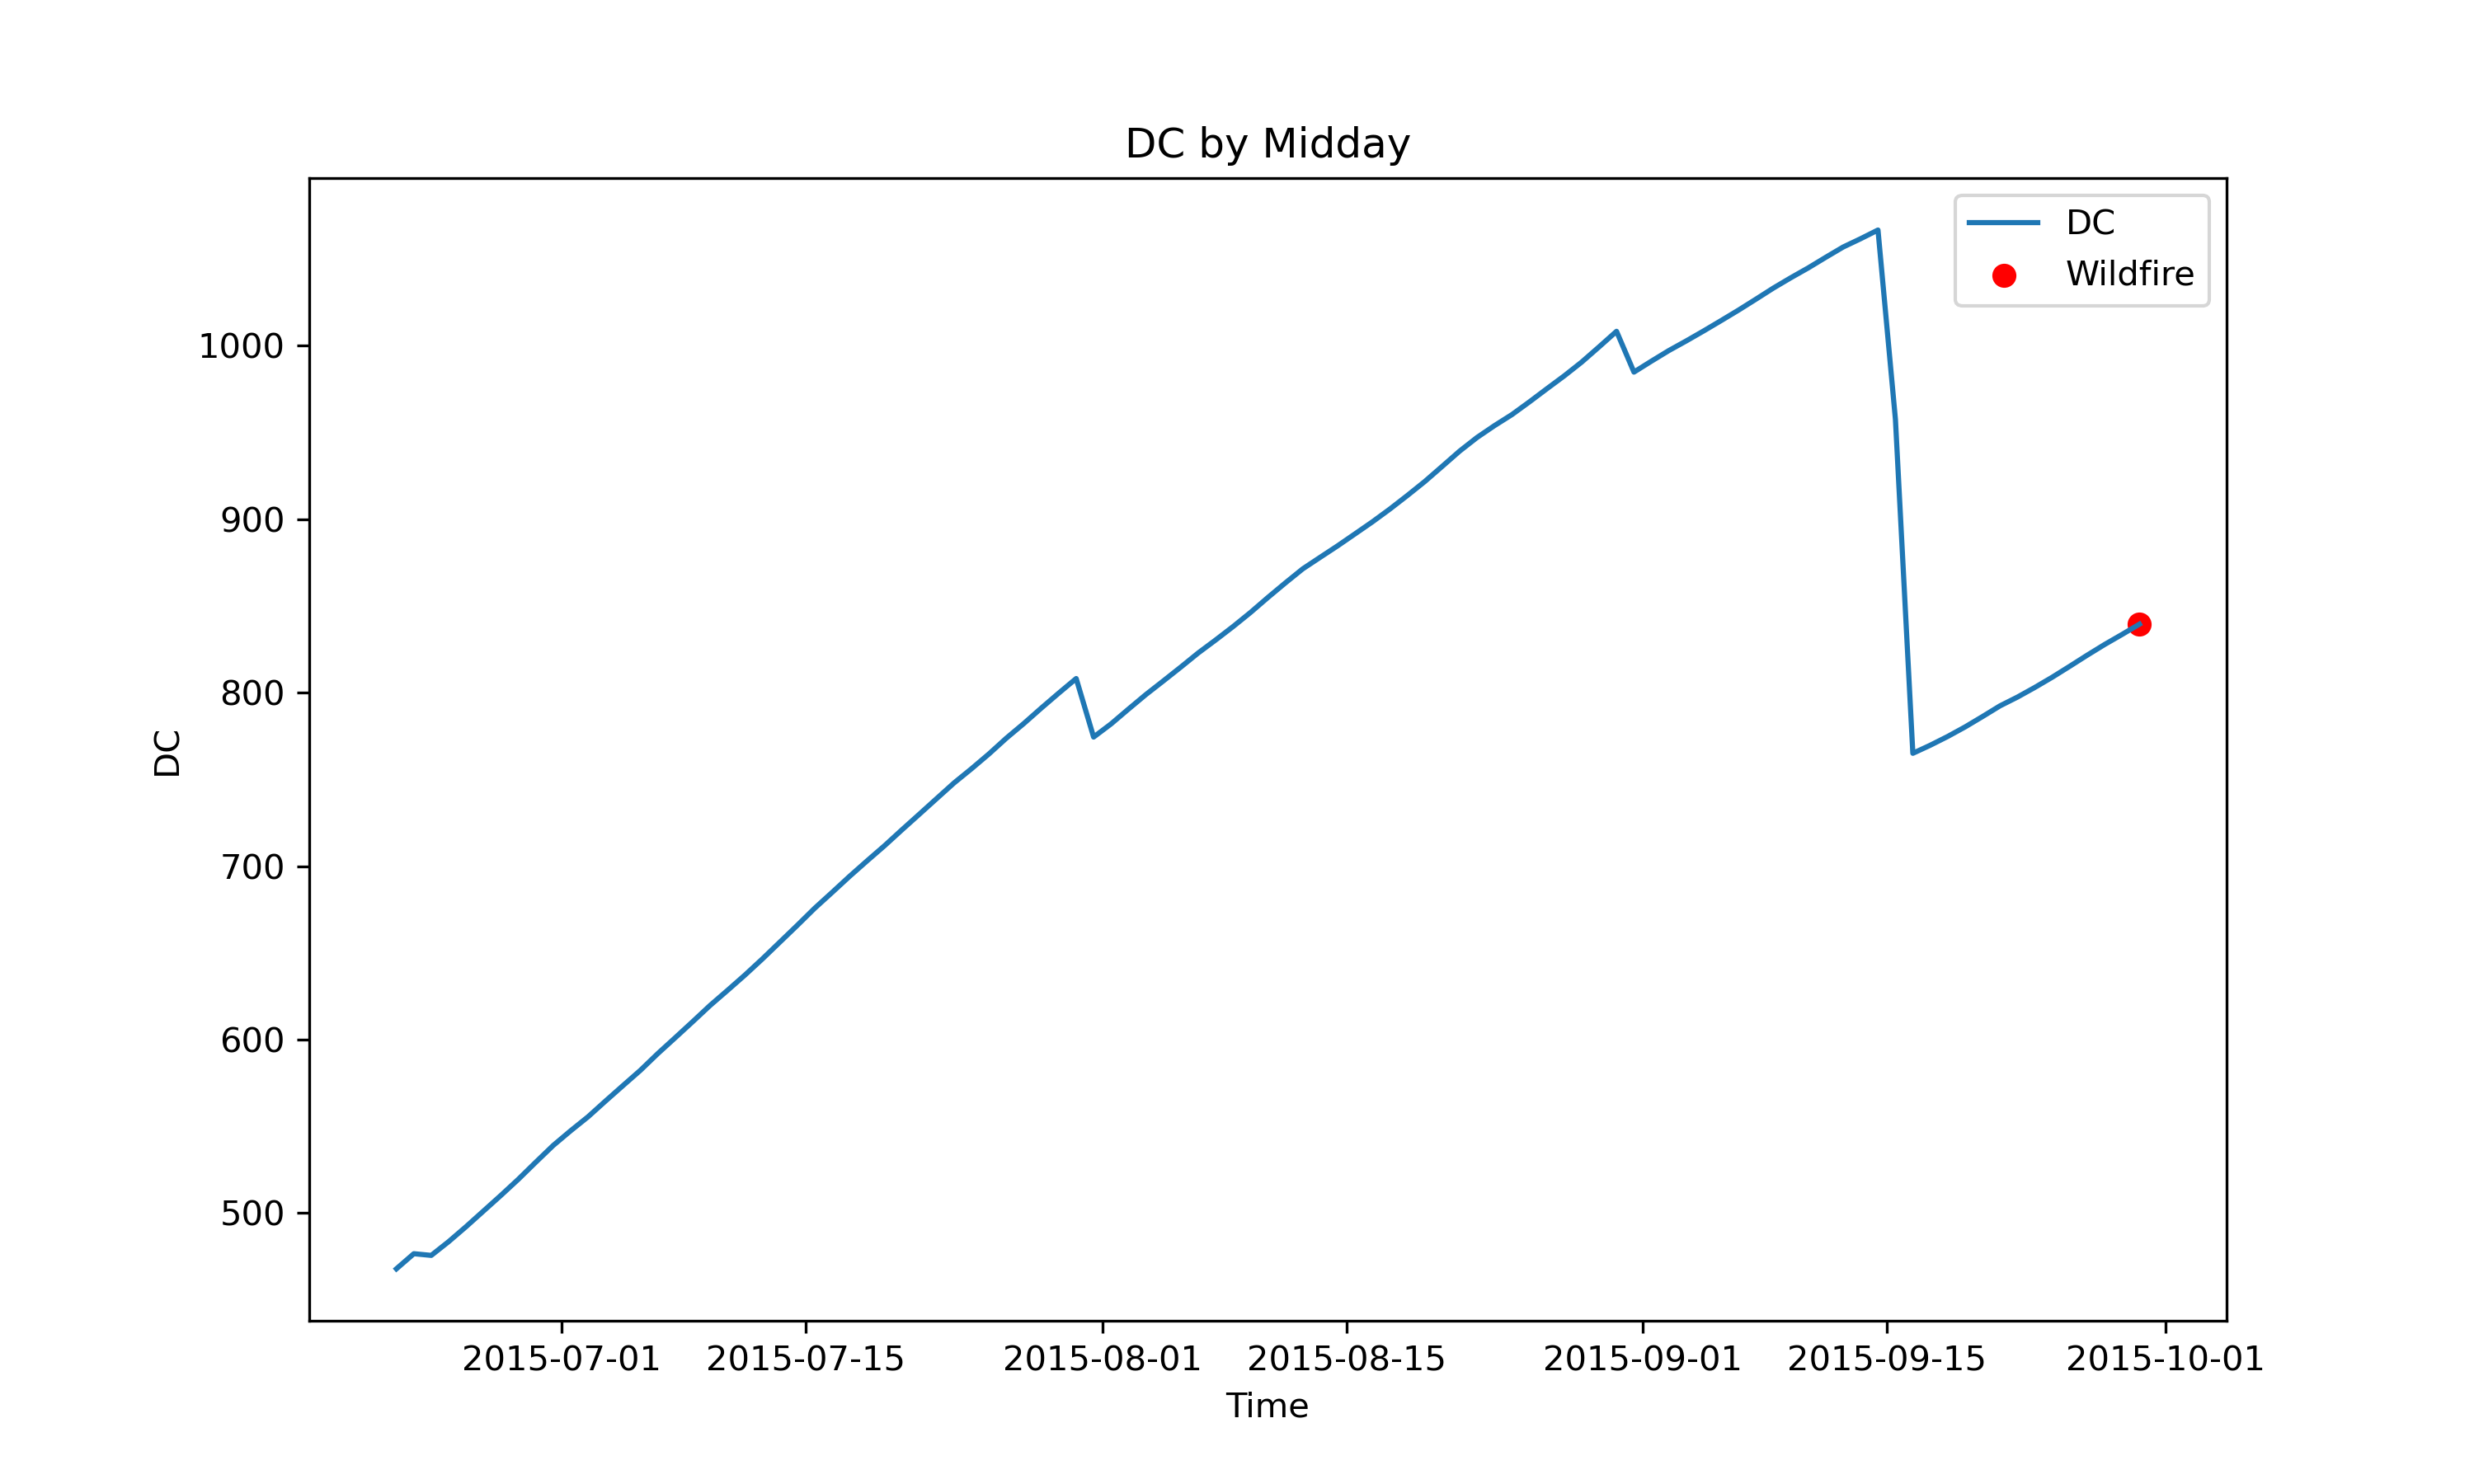
\includegraphics[width=\textwidth]{graphs/2015MesmoSitio/2015CalcDC12.png}
        \caption{DC - Calculated value}
        \label{fig:dc_calculated_2015_semfogo}
    \end{subfigure}
    \label{fig:comparison_dc_semfogo_copernicus_calculated}
\end{figure}

\begin{figure}[h]
\caption{Comparison of ISI calculated values and Copernicus}
    \centering
    \begin{subfigure}{0.49\textwidth}
        \centering
        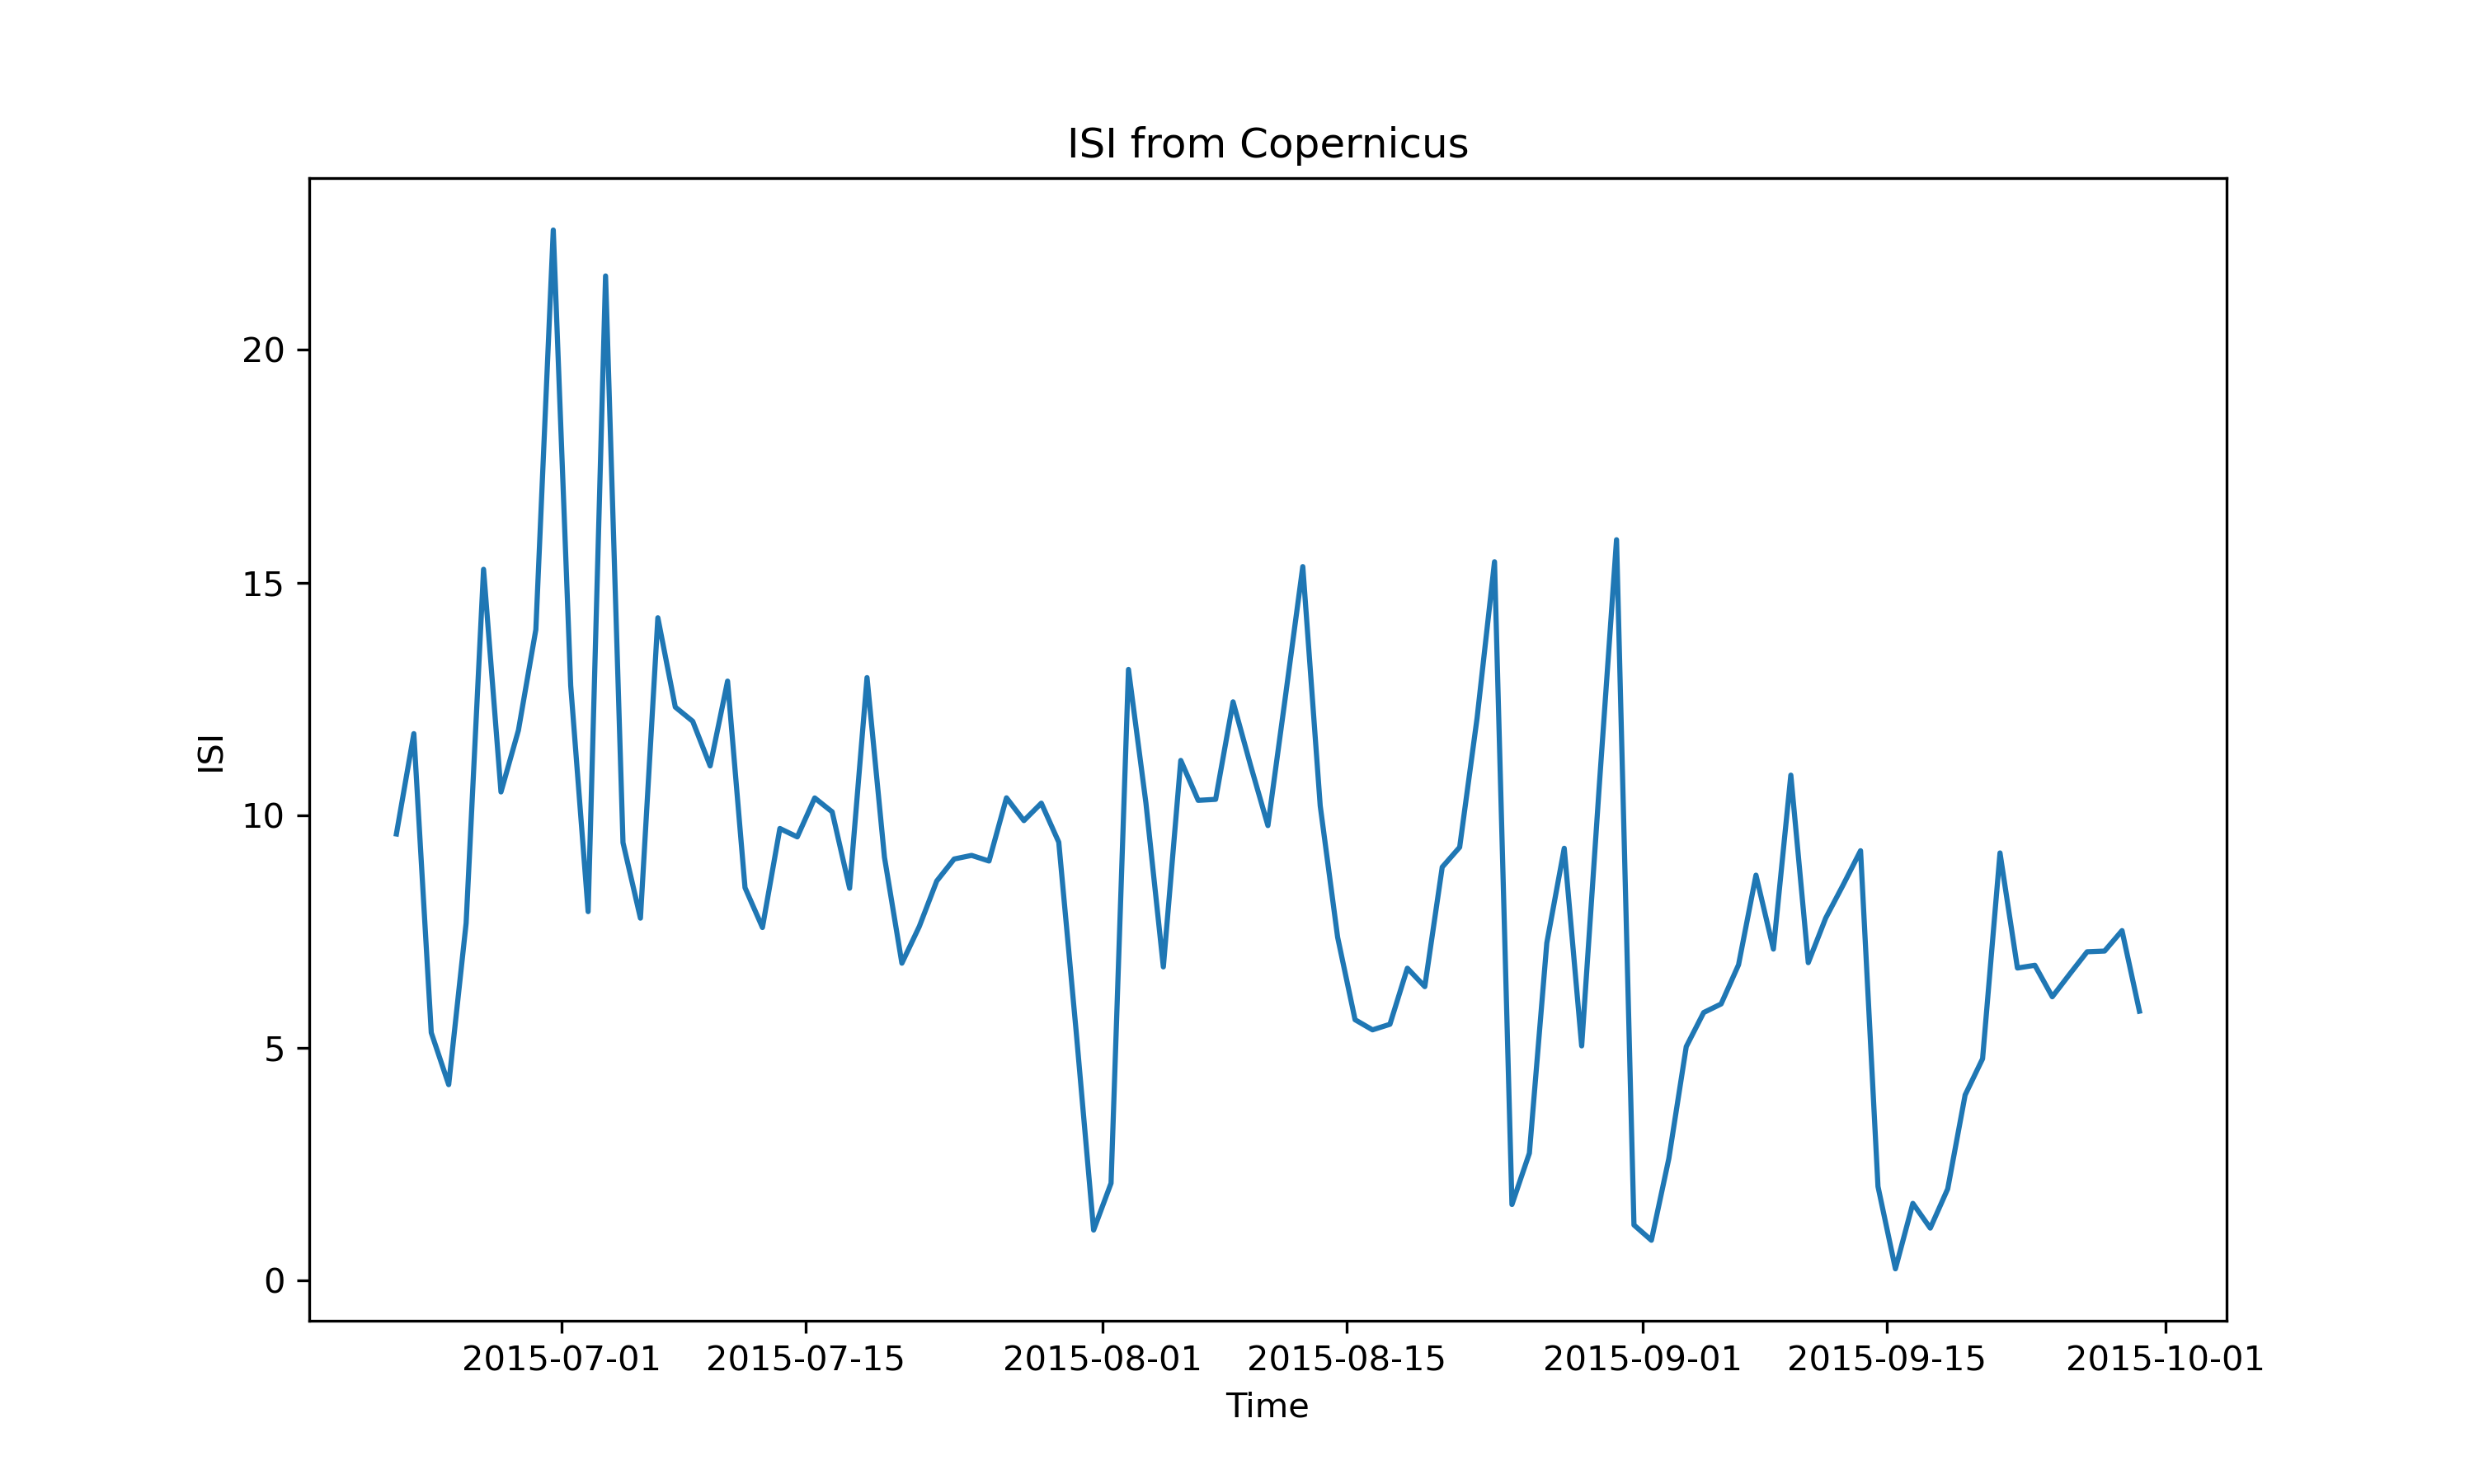
\includegraphics[width=\textwidth]{graphs/2015MesmoSitio/2015CopernicusISI12.png}
        \caption{ISI - Copernicus}
        \label{fig:isi_copernicus_2015_semfogo}
    \end{subfigure}
    \hfill
    \begin{subfigure}{0.49\textwidth}
        \centering
        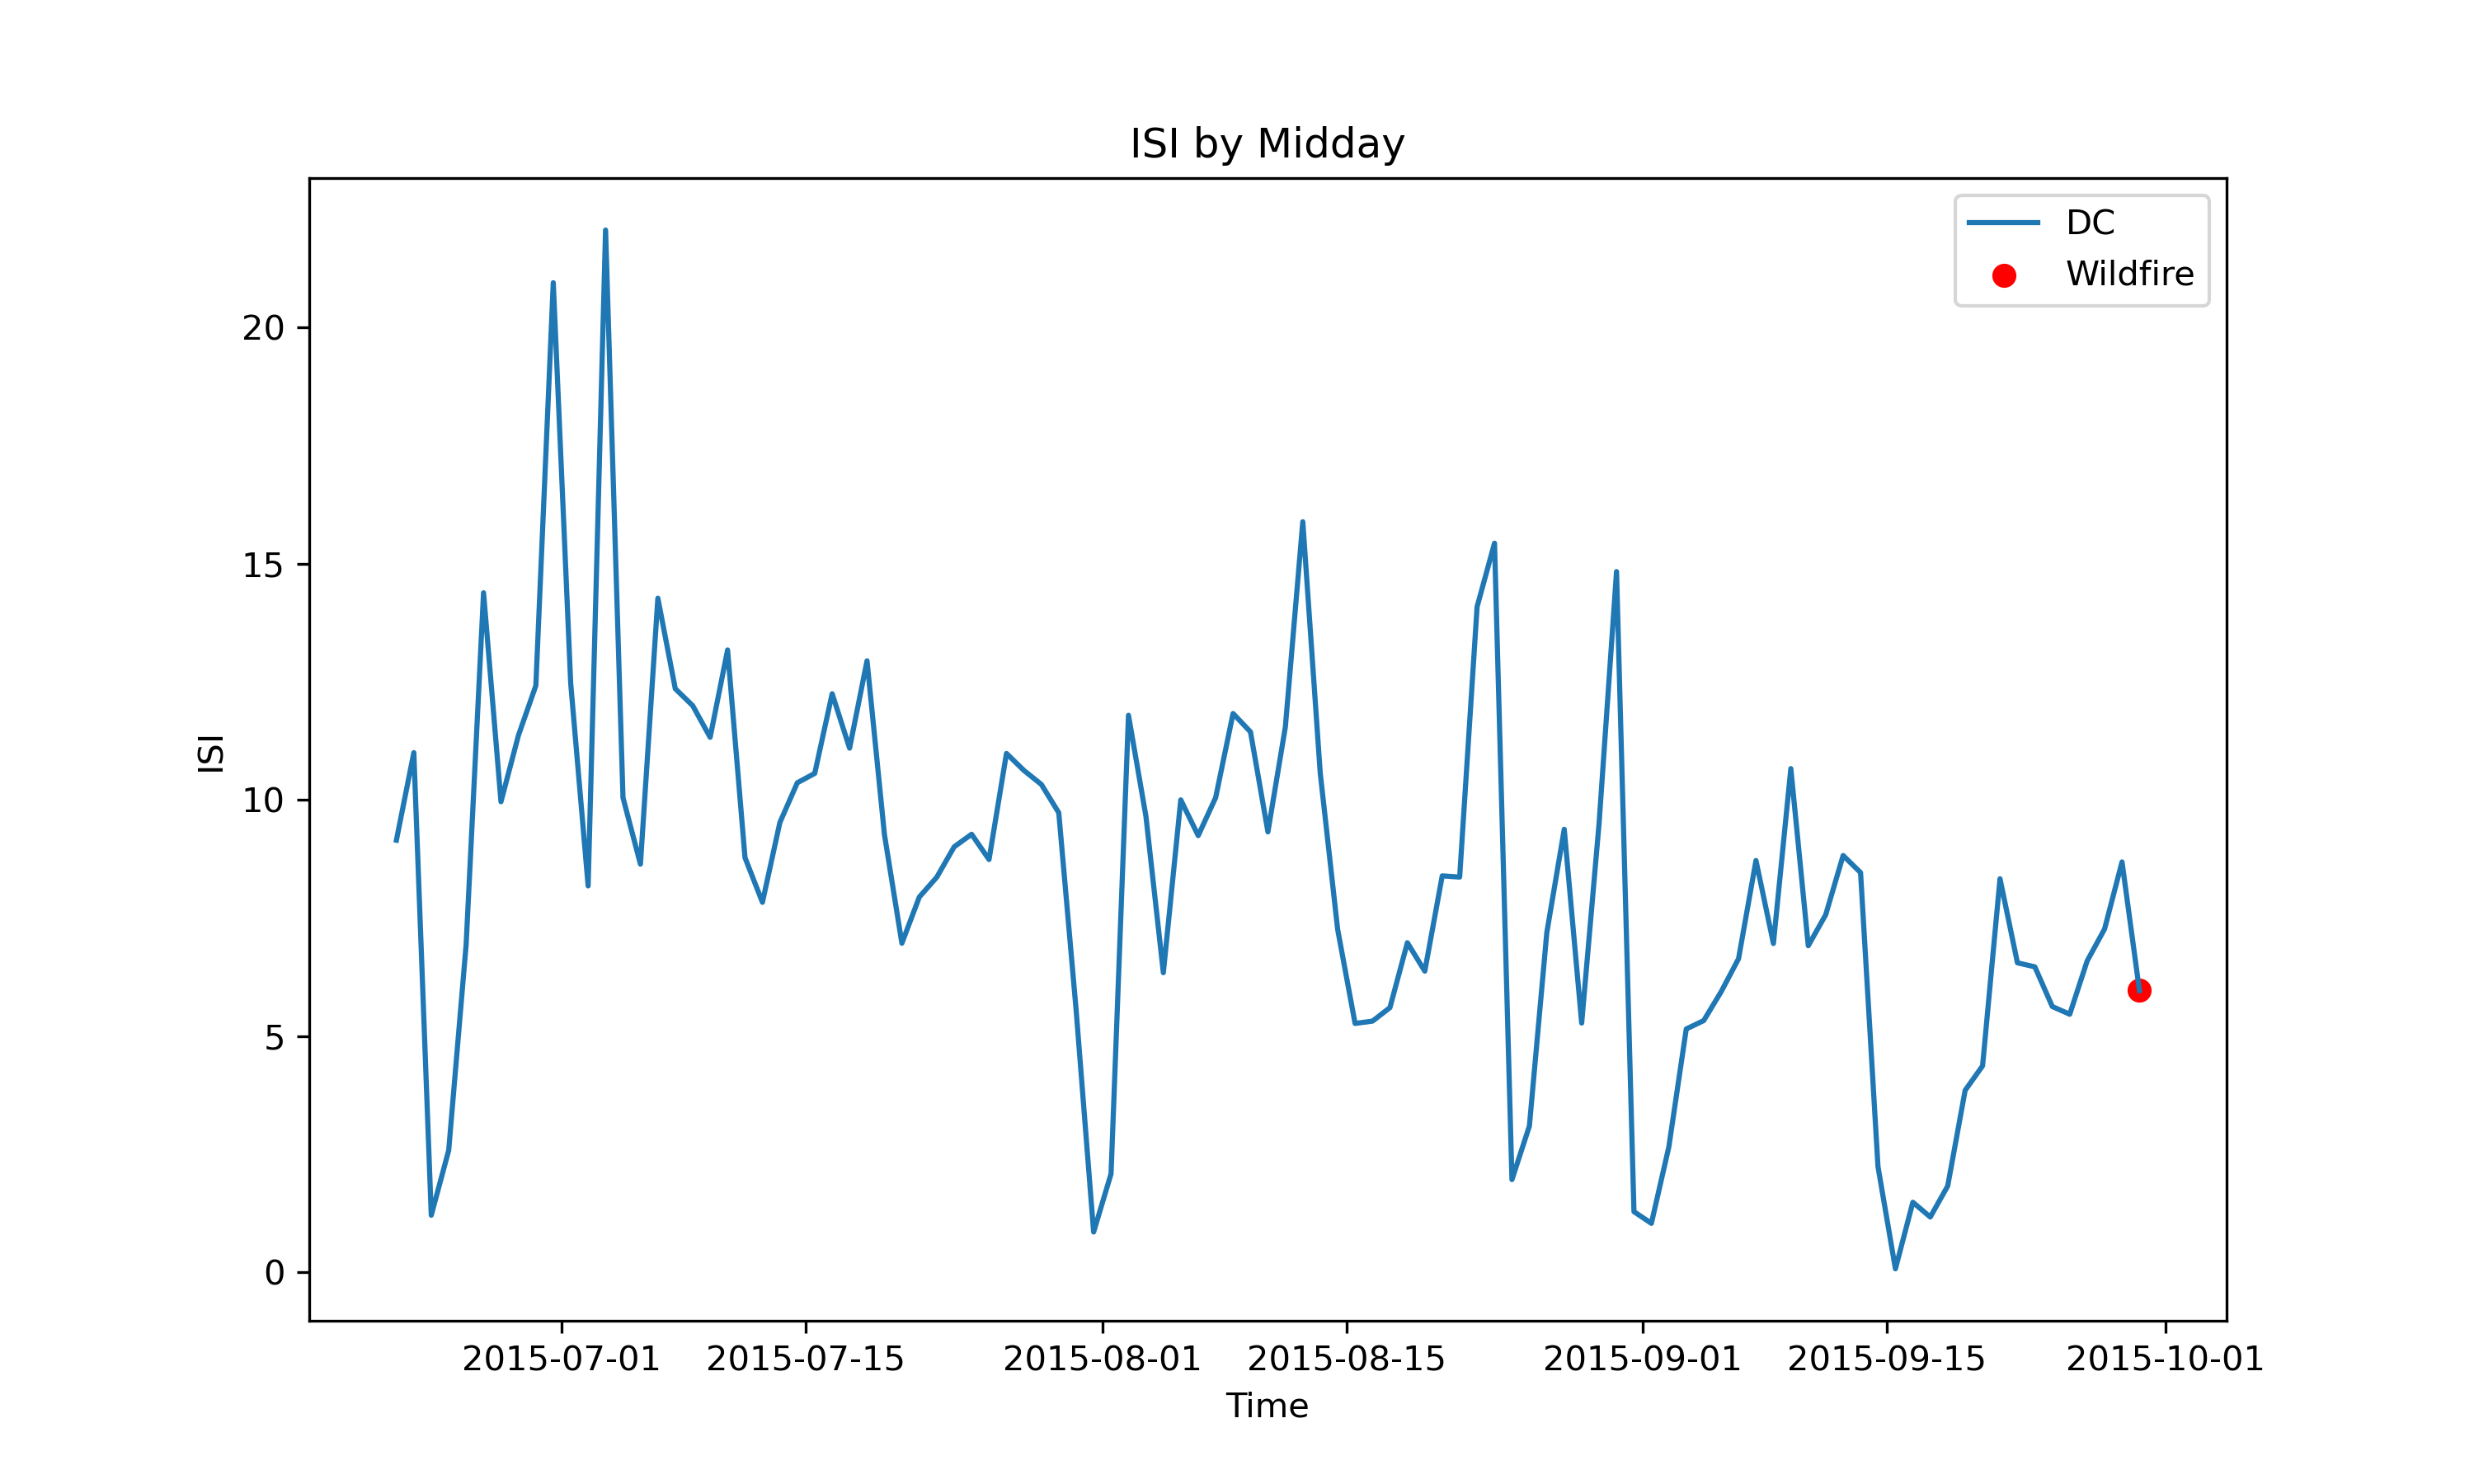
\includegraphics[width=\textwidth]{graphs/2015MesmoSitio/2015CalcISI12.png}
        \caption{ISI - Calculated value}
        \label{fig:isi_calculated_2015_semfogo}
    \end{subfigure}
    \label{fig:comparison_isi_semfogo_copernicus_calculated}
\end{figure}

\begin{figure}[h]
\caption{Comparison of BUI calculated values and Copernicus}
    \centering
    \begin{subfigure}{0.49\textwidth}
        \centering
        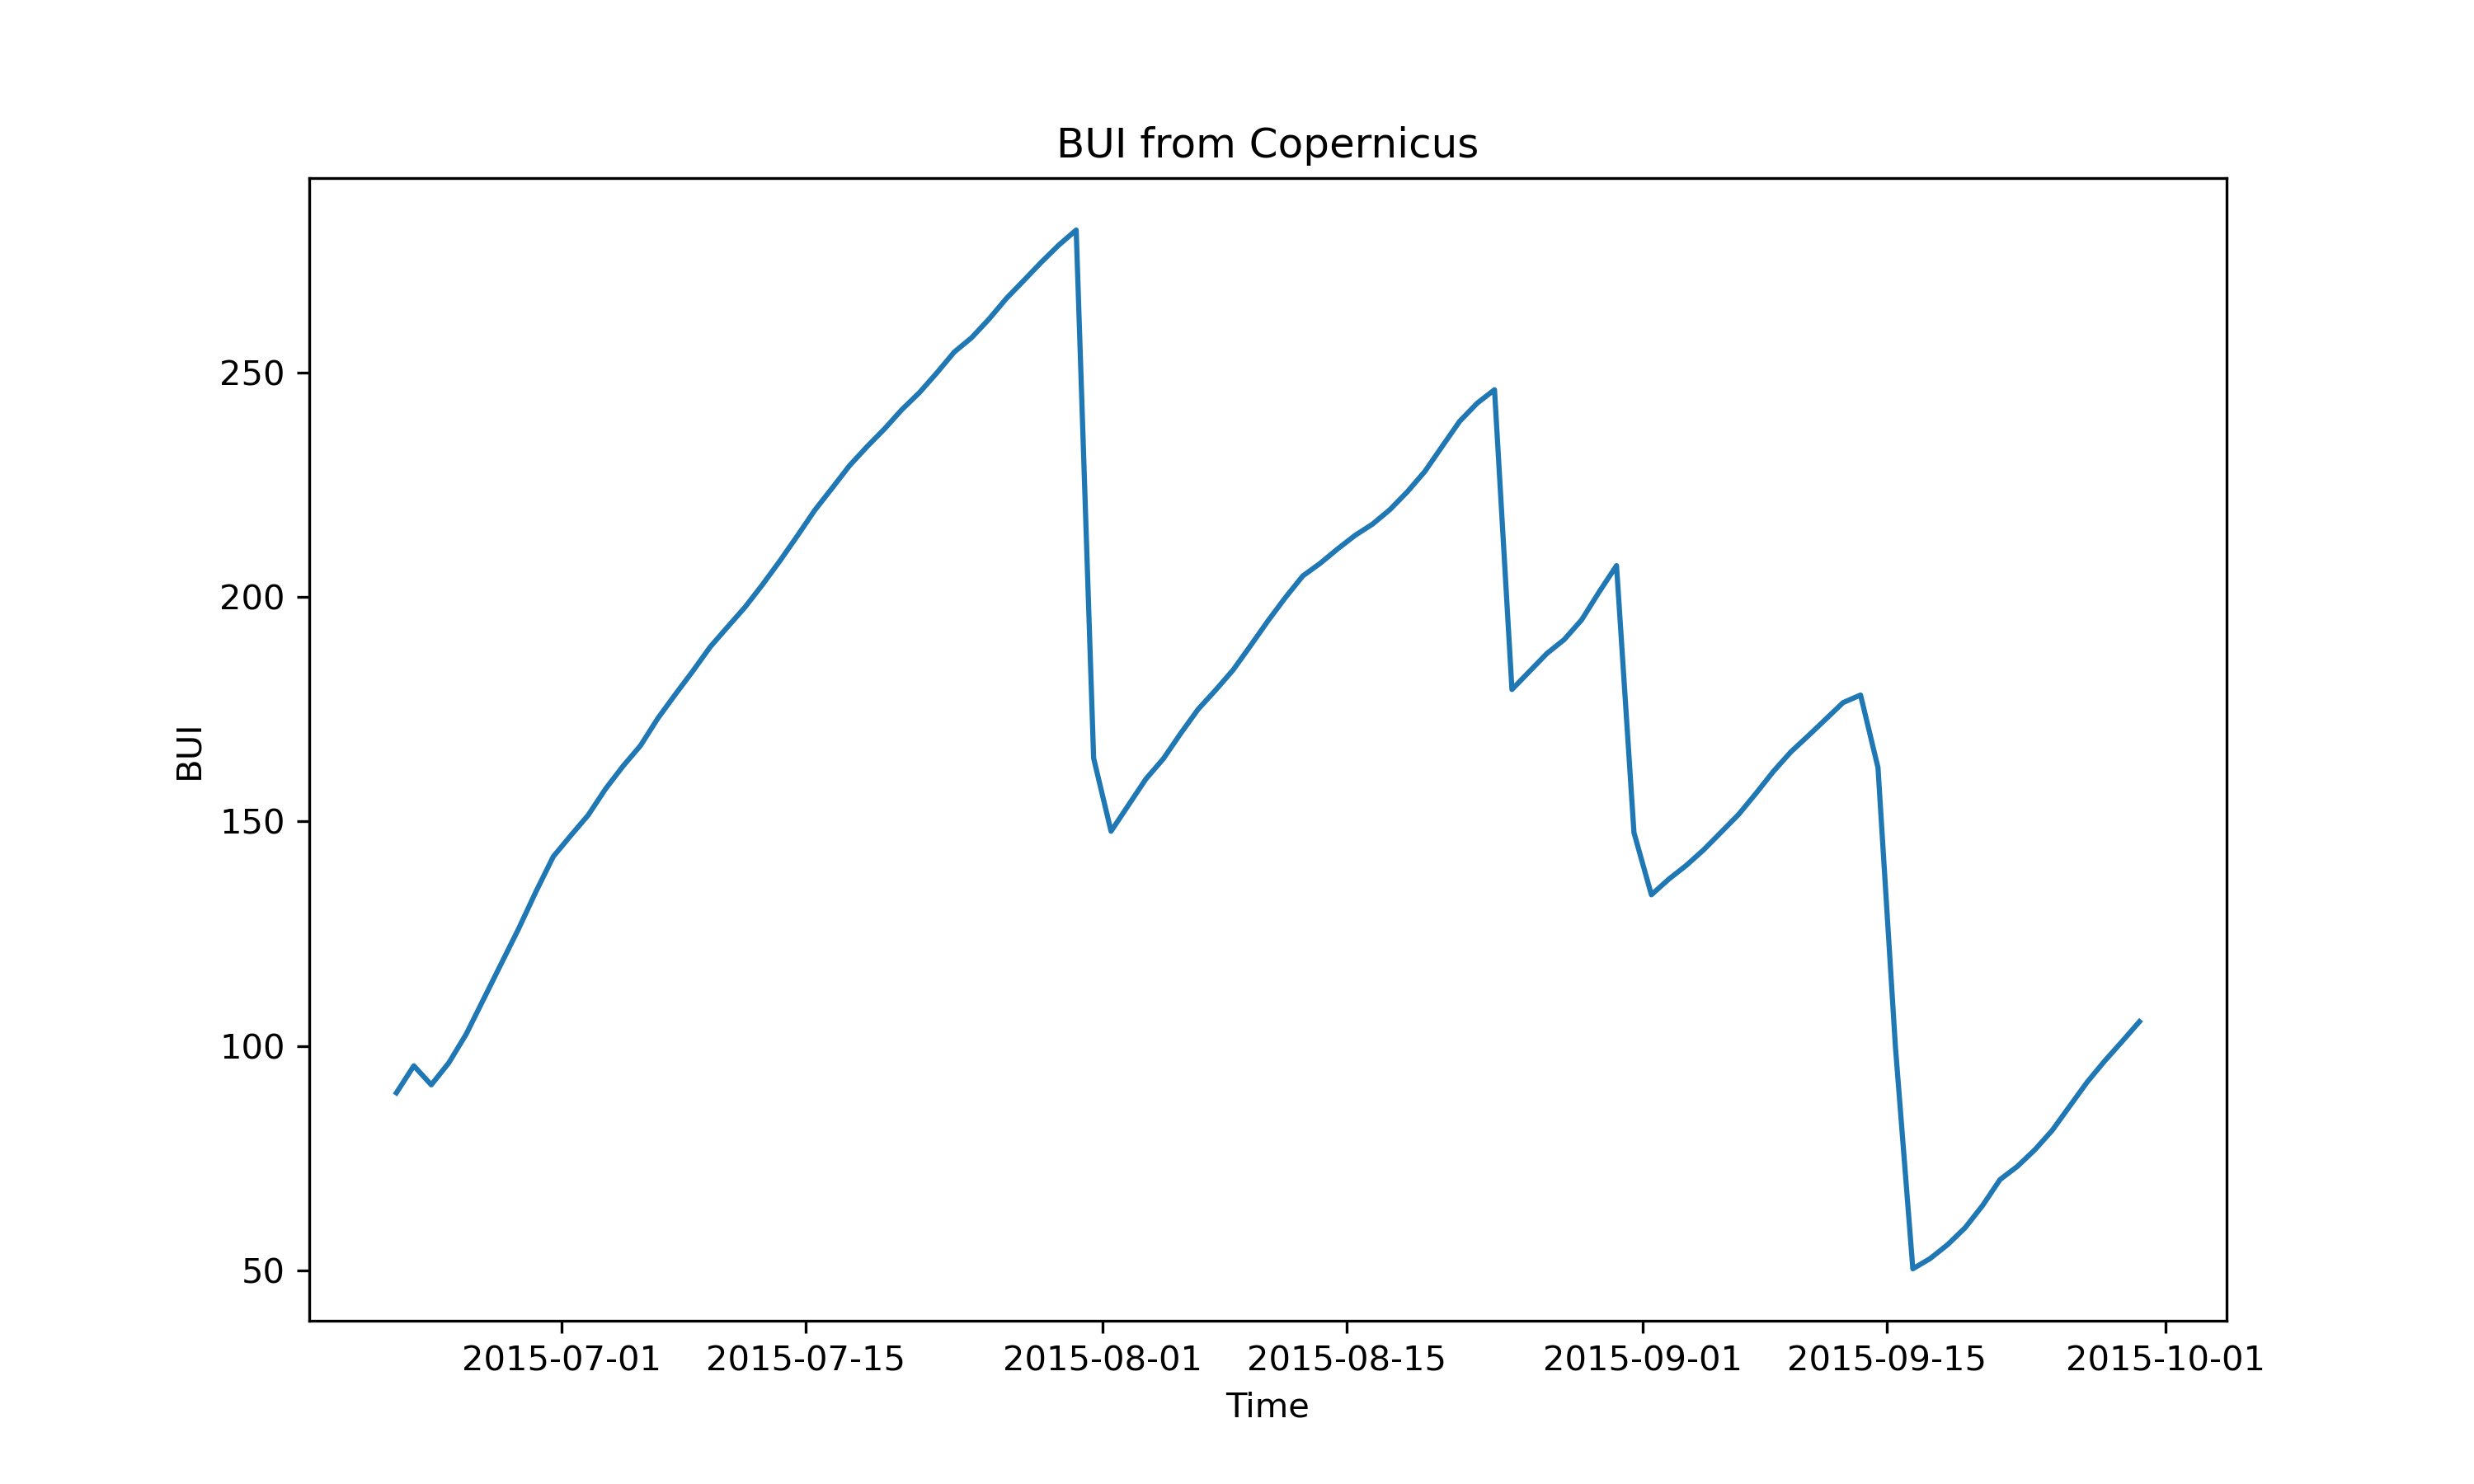
\includegraphics[width=\textwidth]{graphs/2015MesmoSitio/2015CopernicusBUI12.png}
        \caption{BUI - Copernicus}
        \label{fig:bui_copernicus_2015_semfogo}
    \end{subfigure}
    \hfill
    \begin{subfigure}{0.49\textwidth}
        \centering
        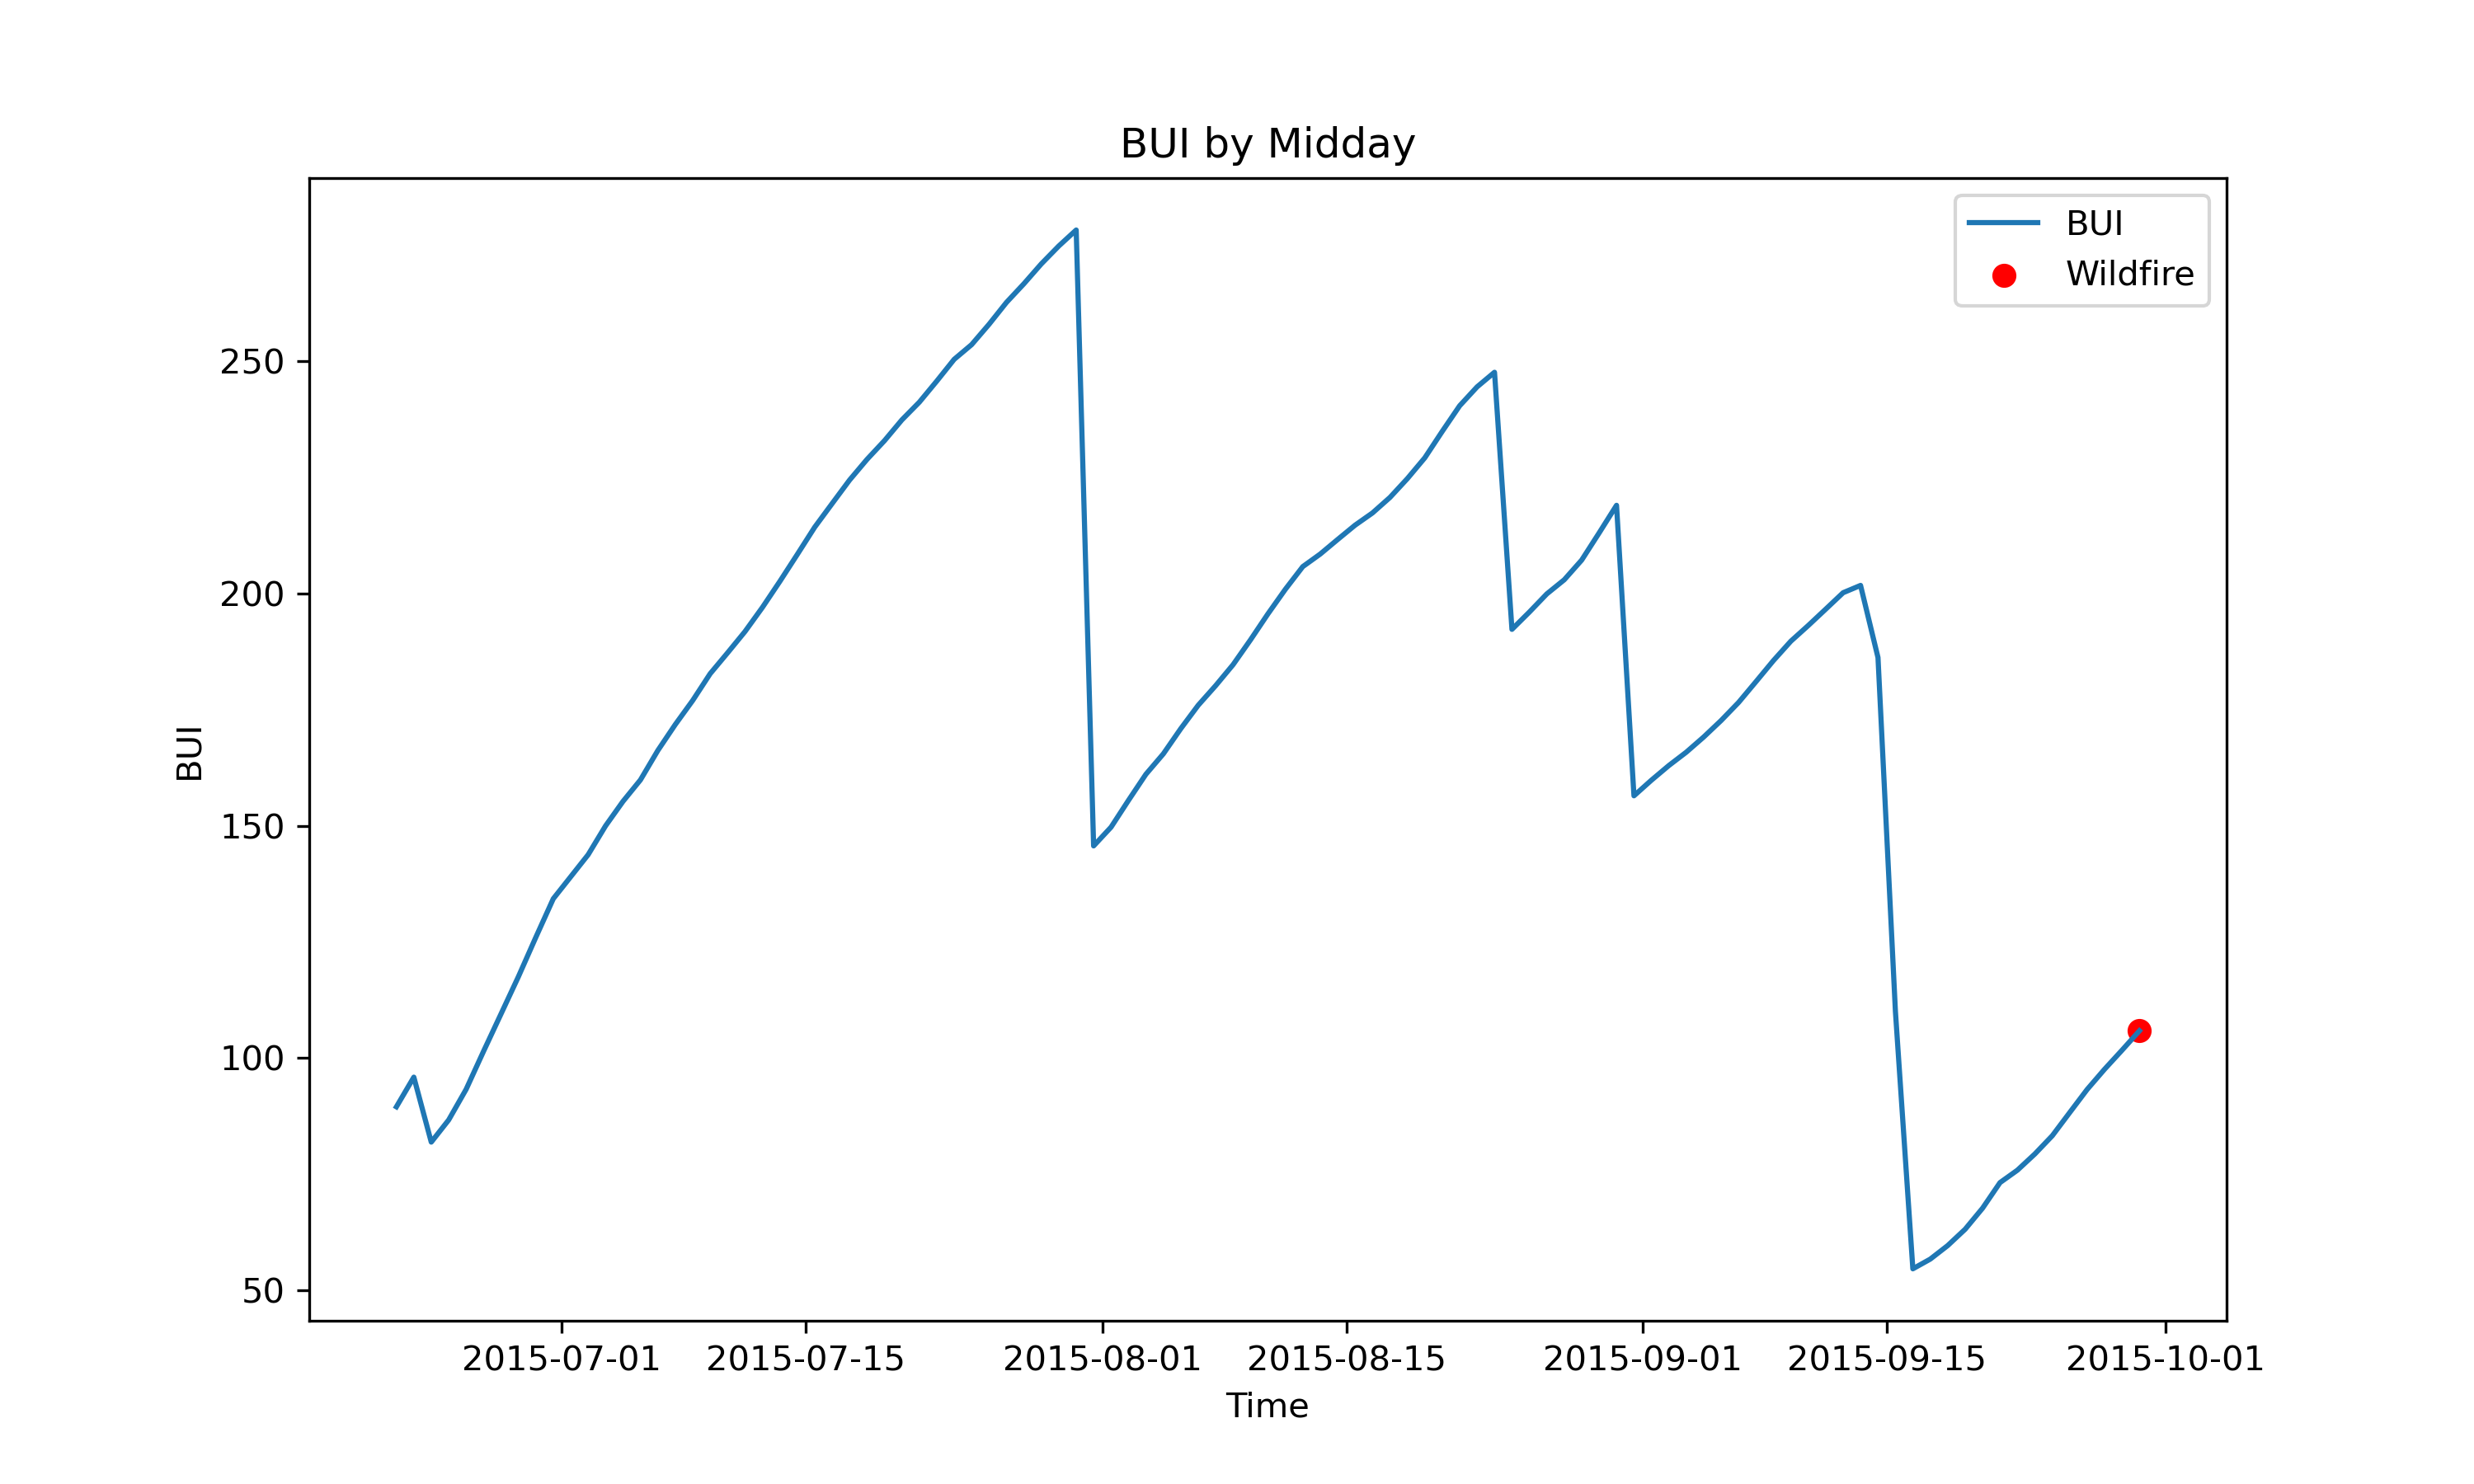
\includegraphics[width=\textwidth]{graphs/2015MesmoSitio/2015CalcBUI12.png}
        \caption{BUI - Calculated value}
        \label{fig:bui_calculated_2015_semfogo}
    \end{subfigure}
    \label{fig:comparison_bui_semfogo_copernicus_calculated}
\end{figure}

\FloatBarrier

\section{Comparison of Copernicus and Simulated FWI}

\subsection{Fogo de 2015}
\begin{figure}[h]
\caption{Comparison of FWI calculated values and Copernicus at midday}
    \centering
    \begin{subfigure}{0.49\textwidth}
        \centering
        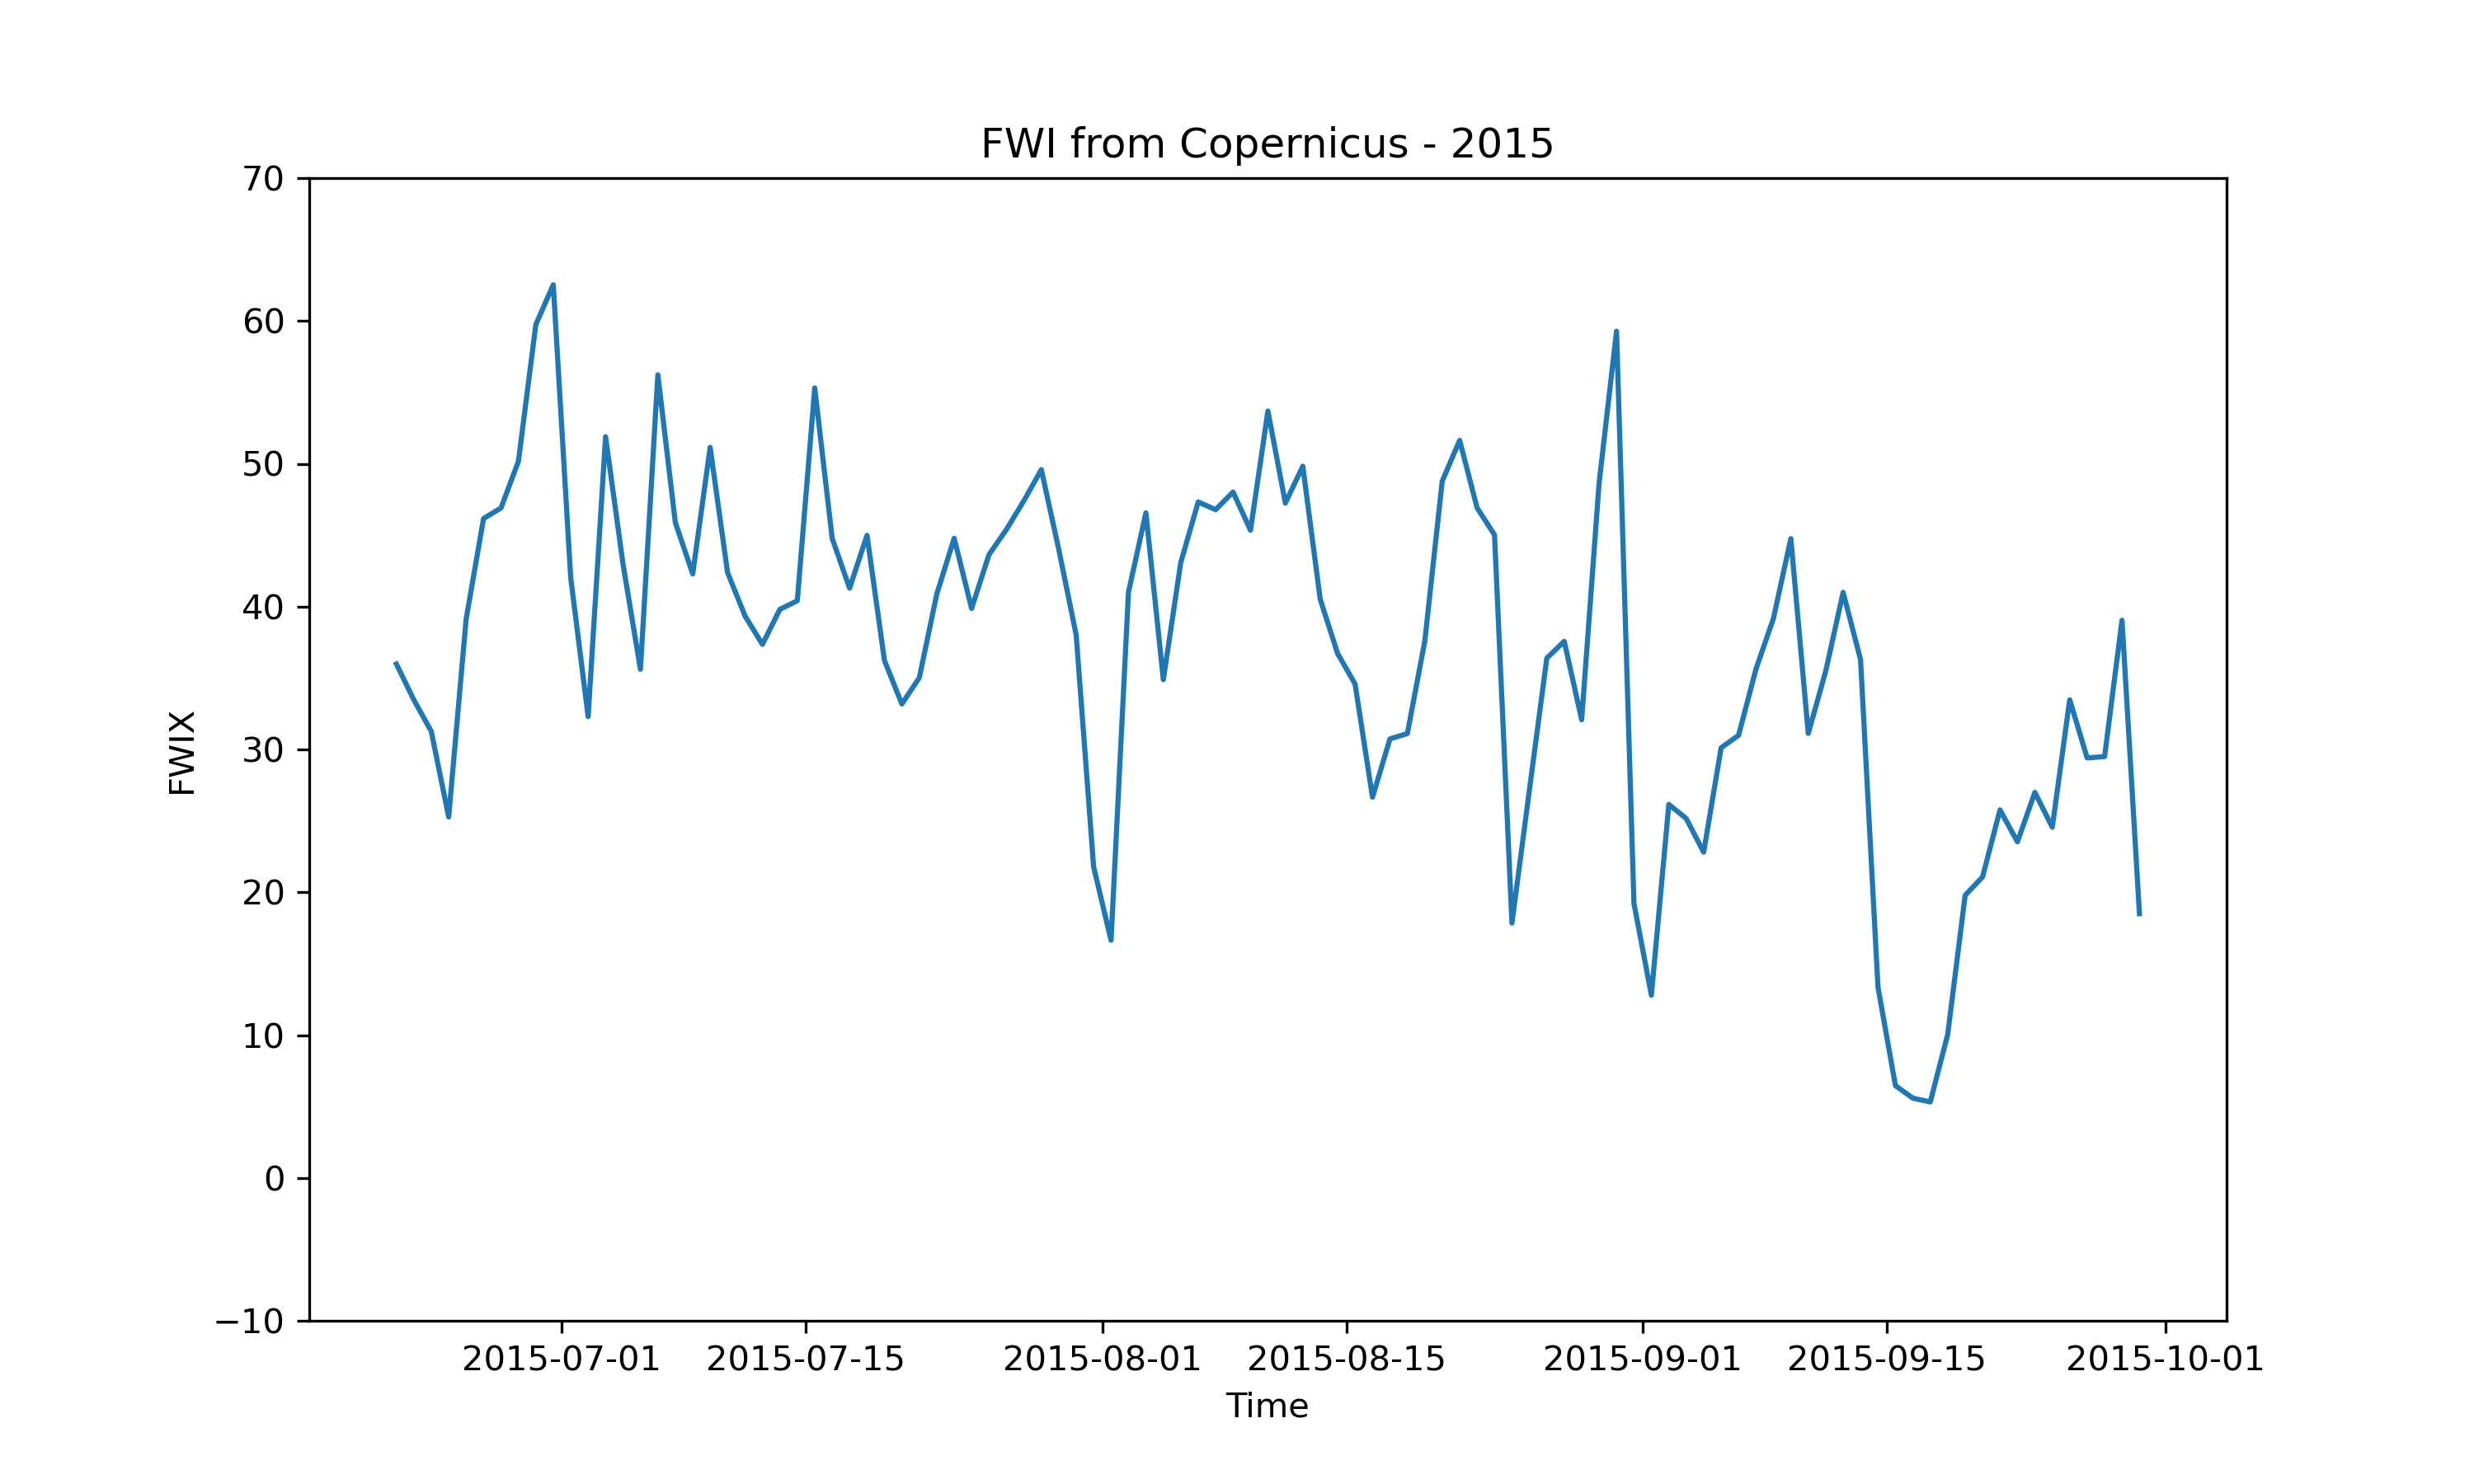
\includegraphics[width=\textwidth]{graphs/2015/2015CopernicusFWI12.png}
        \caption{FWI - Copernicus}
        \label{fig:fwi_copernicus_2015_midday}
    \end{subfigure}
    \hfill
    \begin{subfigure}{0.49\textwidth}
        \centering
        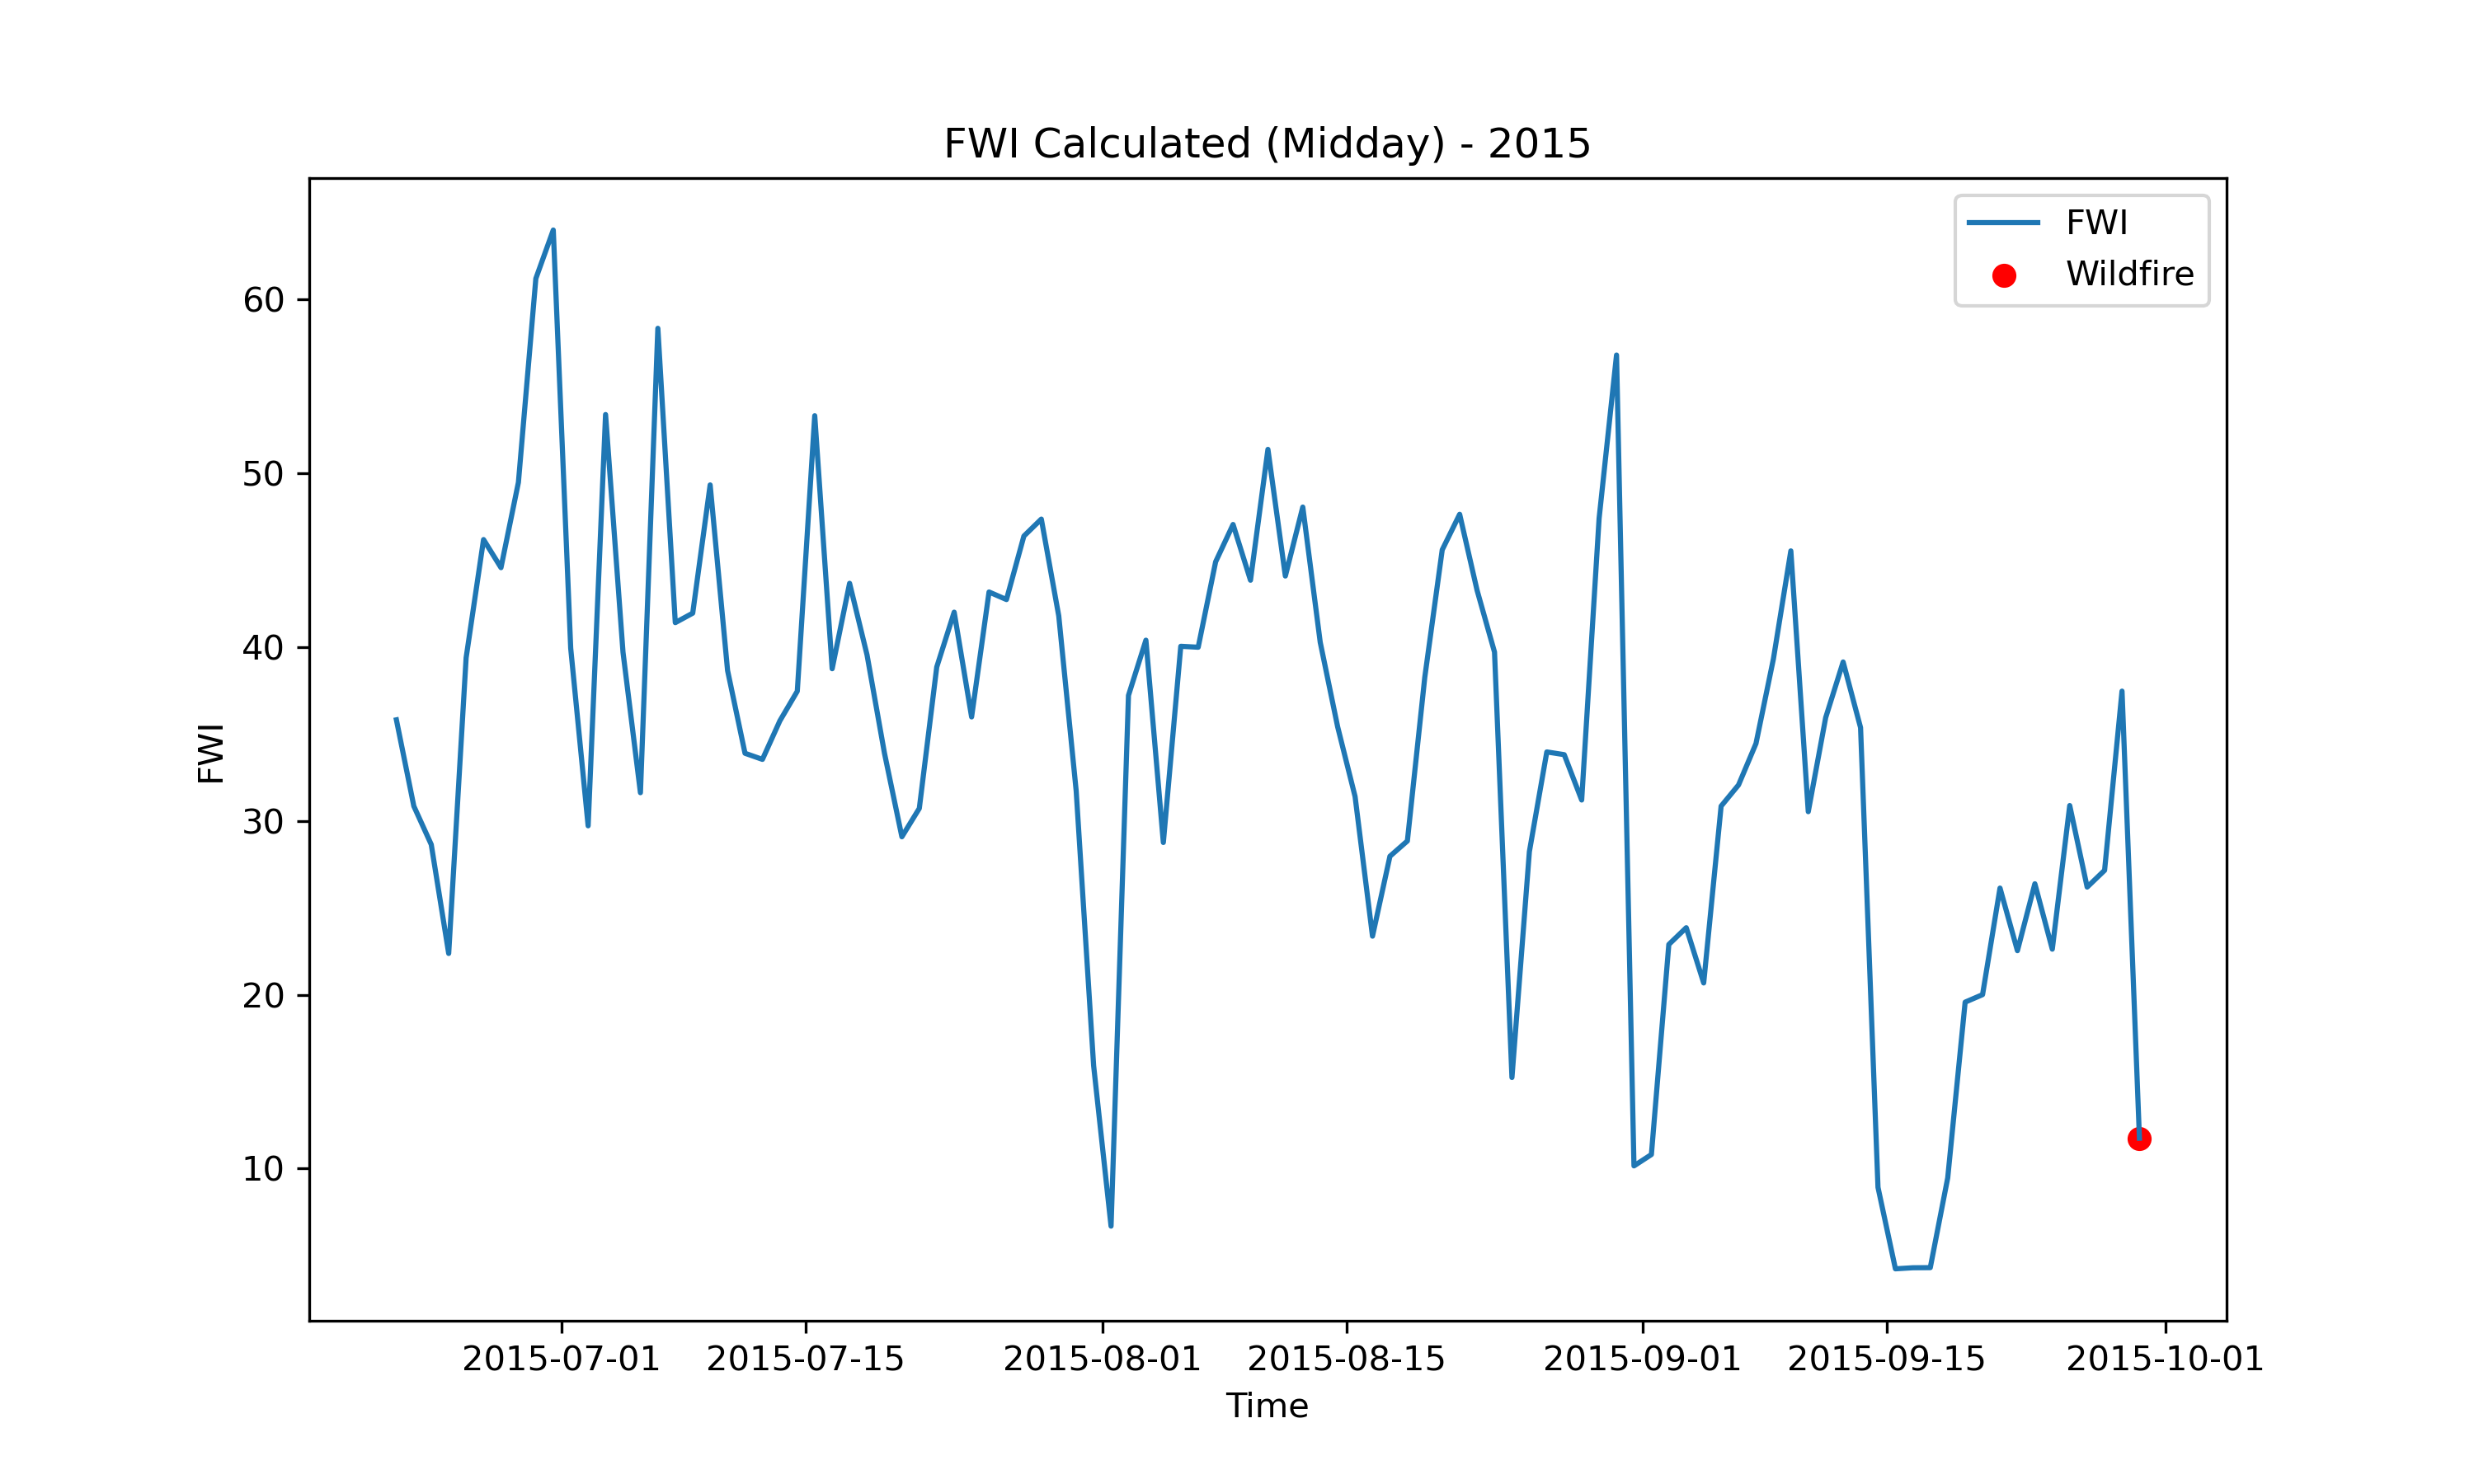
\includegraphics[width=\textwidth]{graphs/2015/2015CalcFWI12.png}
        \caption{FWI - Calculated value}
        \label{fig:fwi_calculated_2015_midday}
    \end{subfigure}
    \label{fig:comparison_fwi_midday_copernicus_calculated}
\end{figure}

\begin{figure}[h]
\caption{Comparison of FFMC calculated values and Copernicus at midday}
    \centering
    \begin{subfigure}{0.49\textwidth}
        \centering
        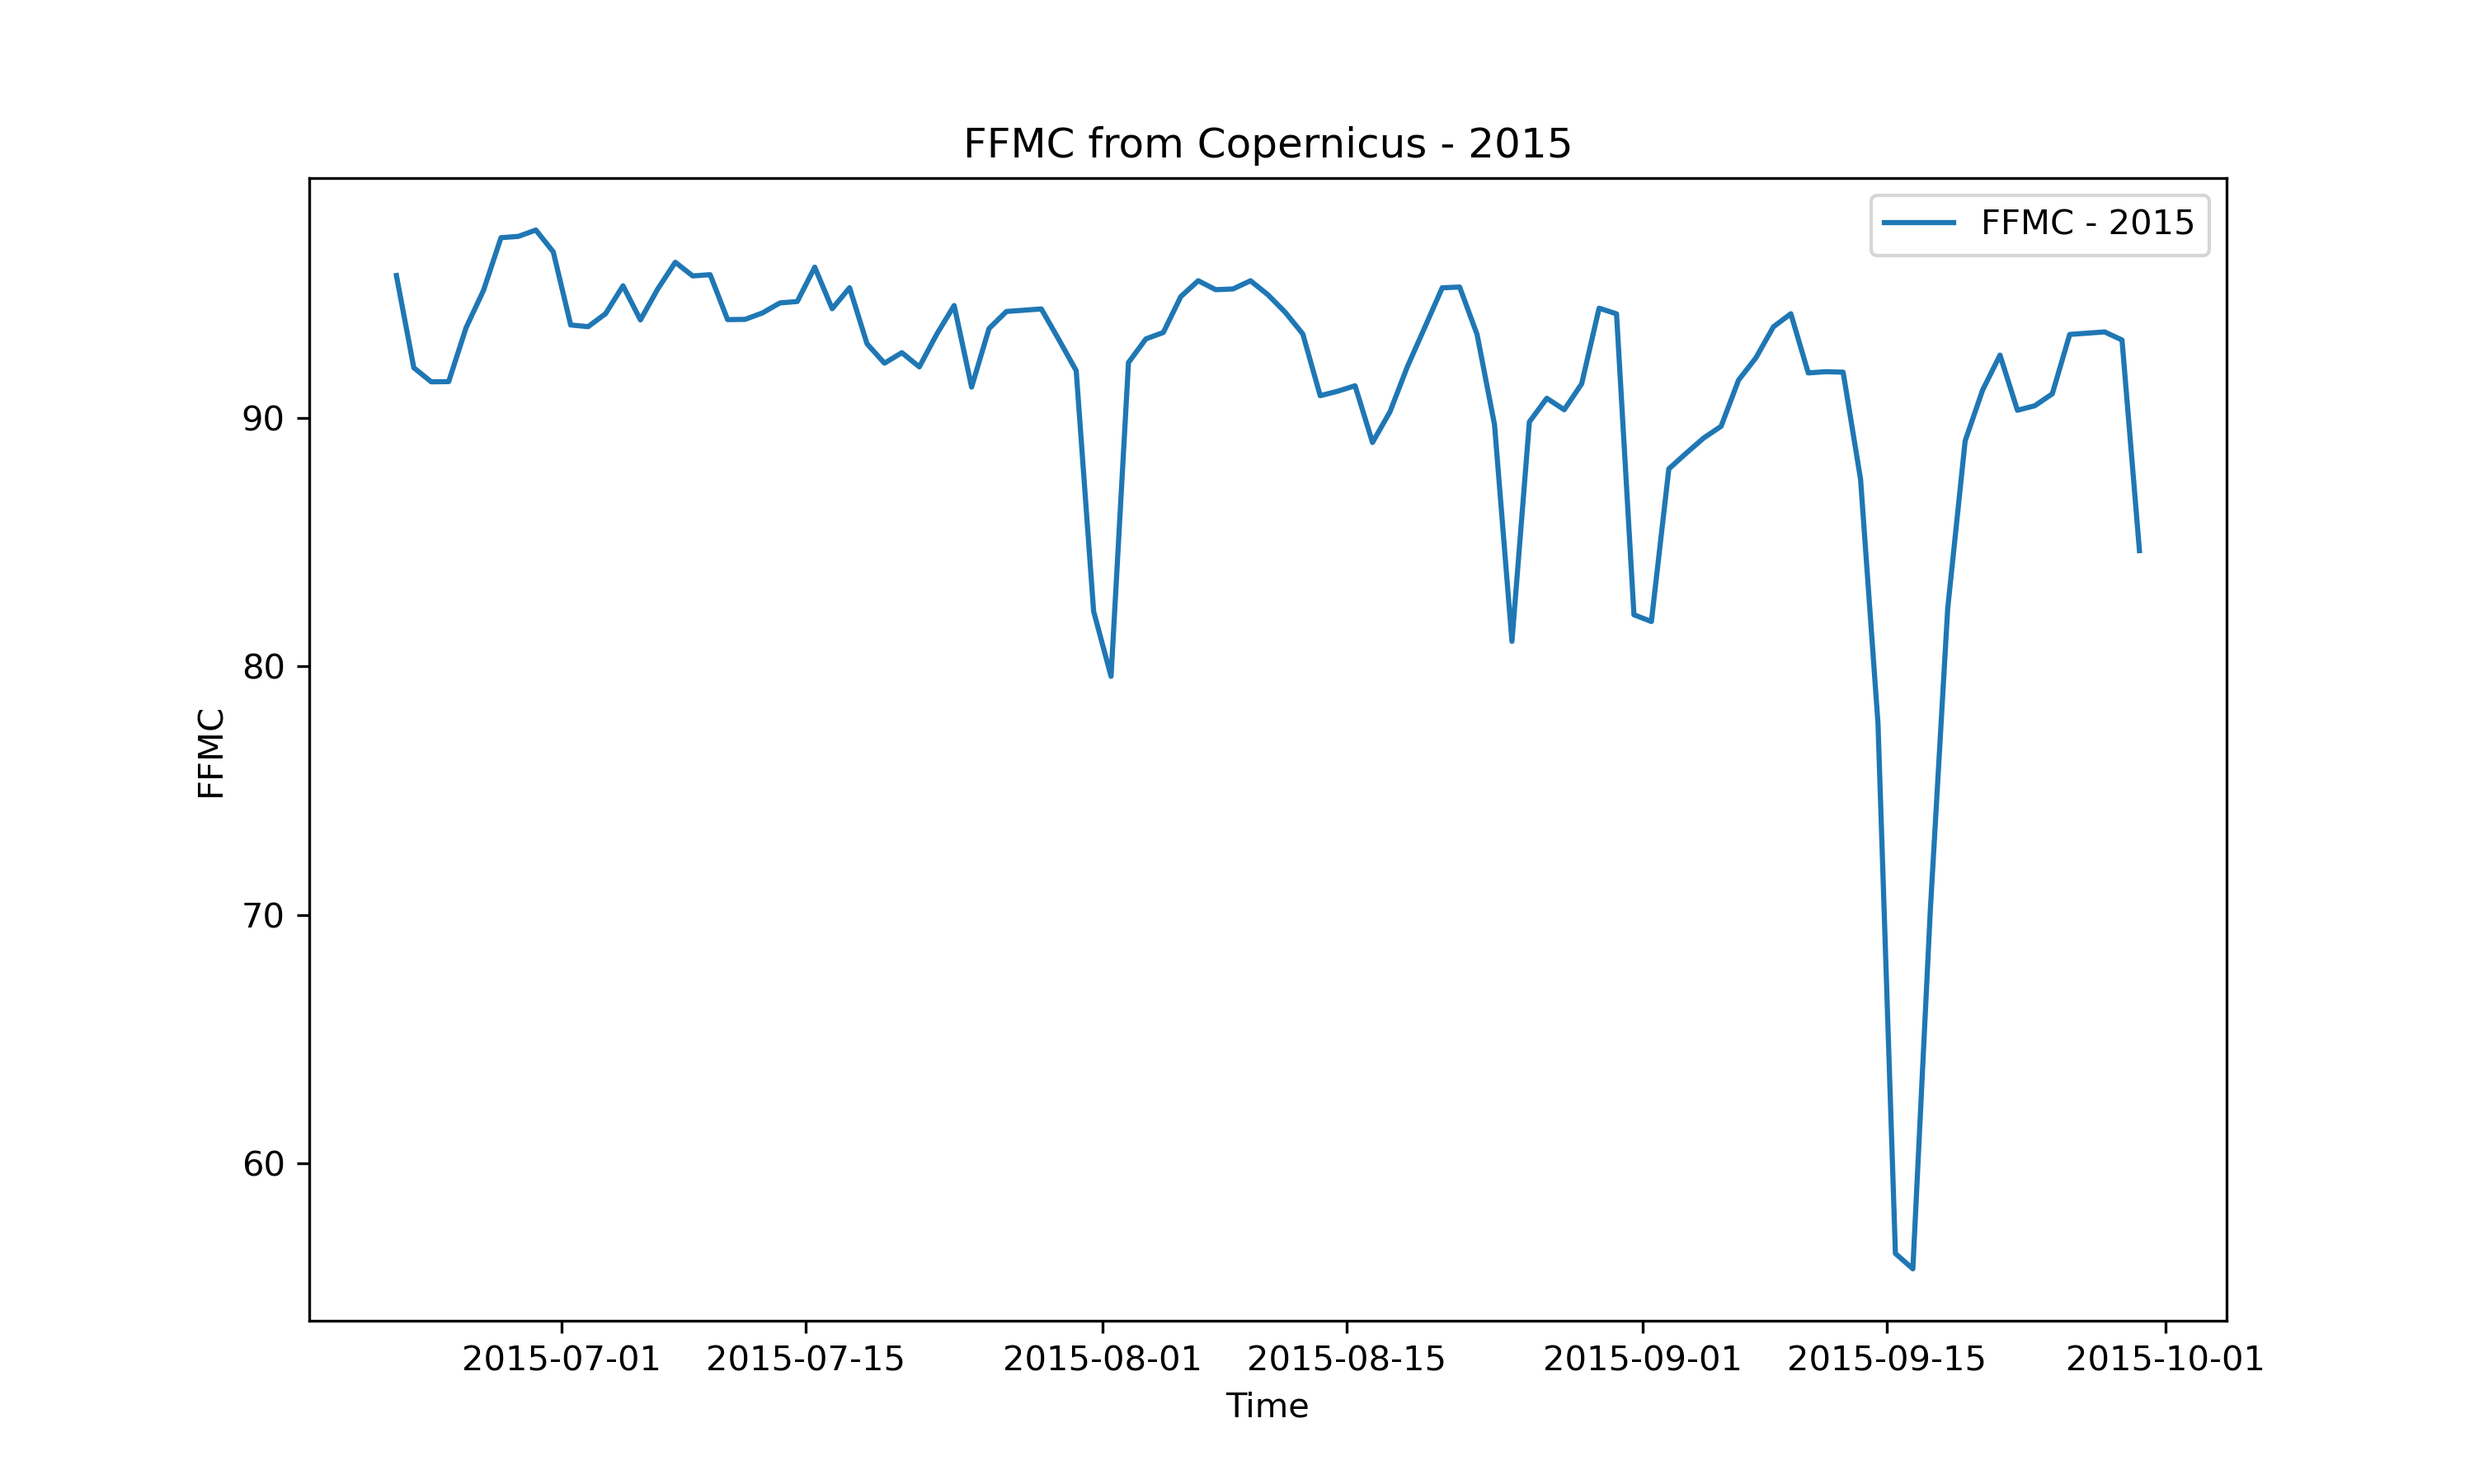
\includegraphics[width=\textwidth]{graphs/2015/2015CopernicusFFMC12.png}
        \caption{FFMC - Copernicus}
        \label{fig:ffmc_copernicus_2015_midday}
    \end{subfigure}
    \hfill
    \begin{subfigure}{0.49\textwidth}
        \centering
        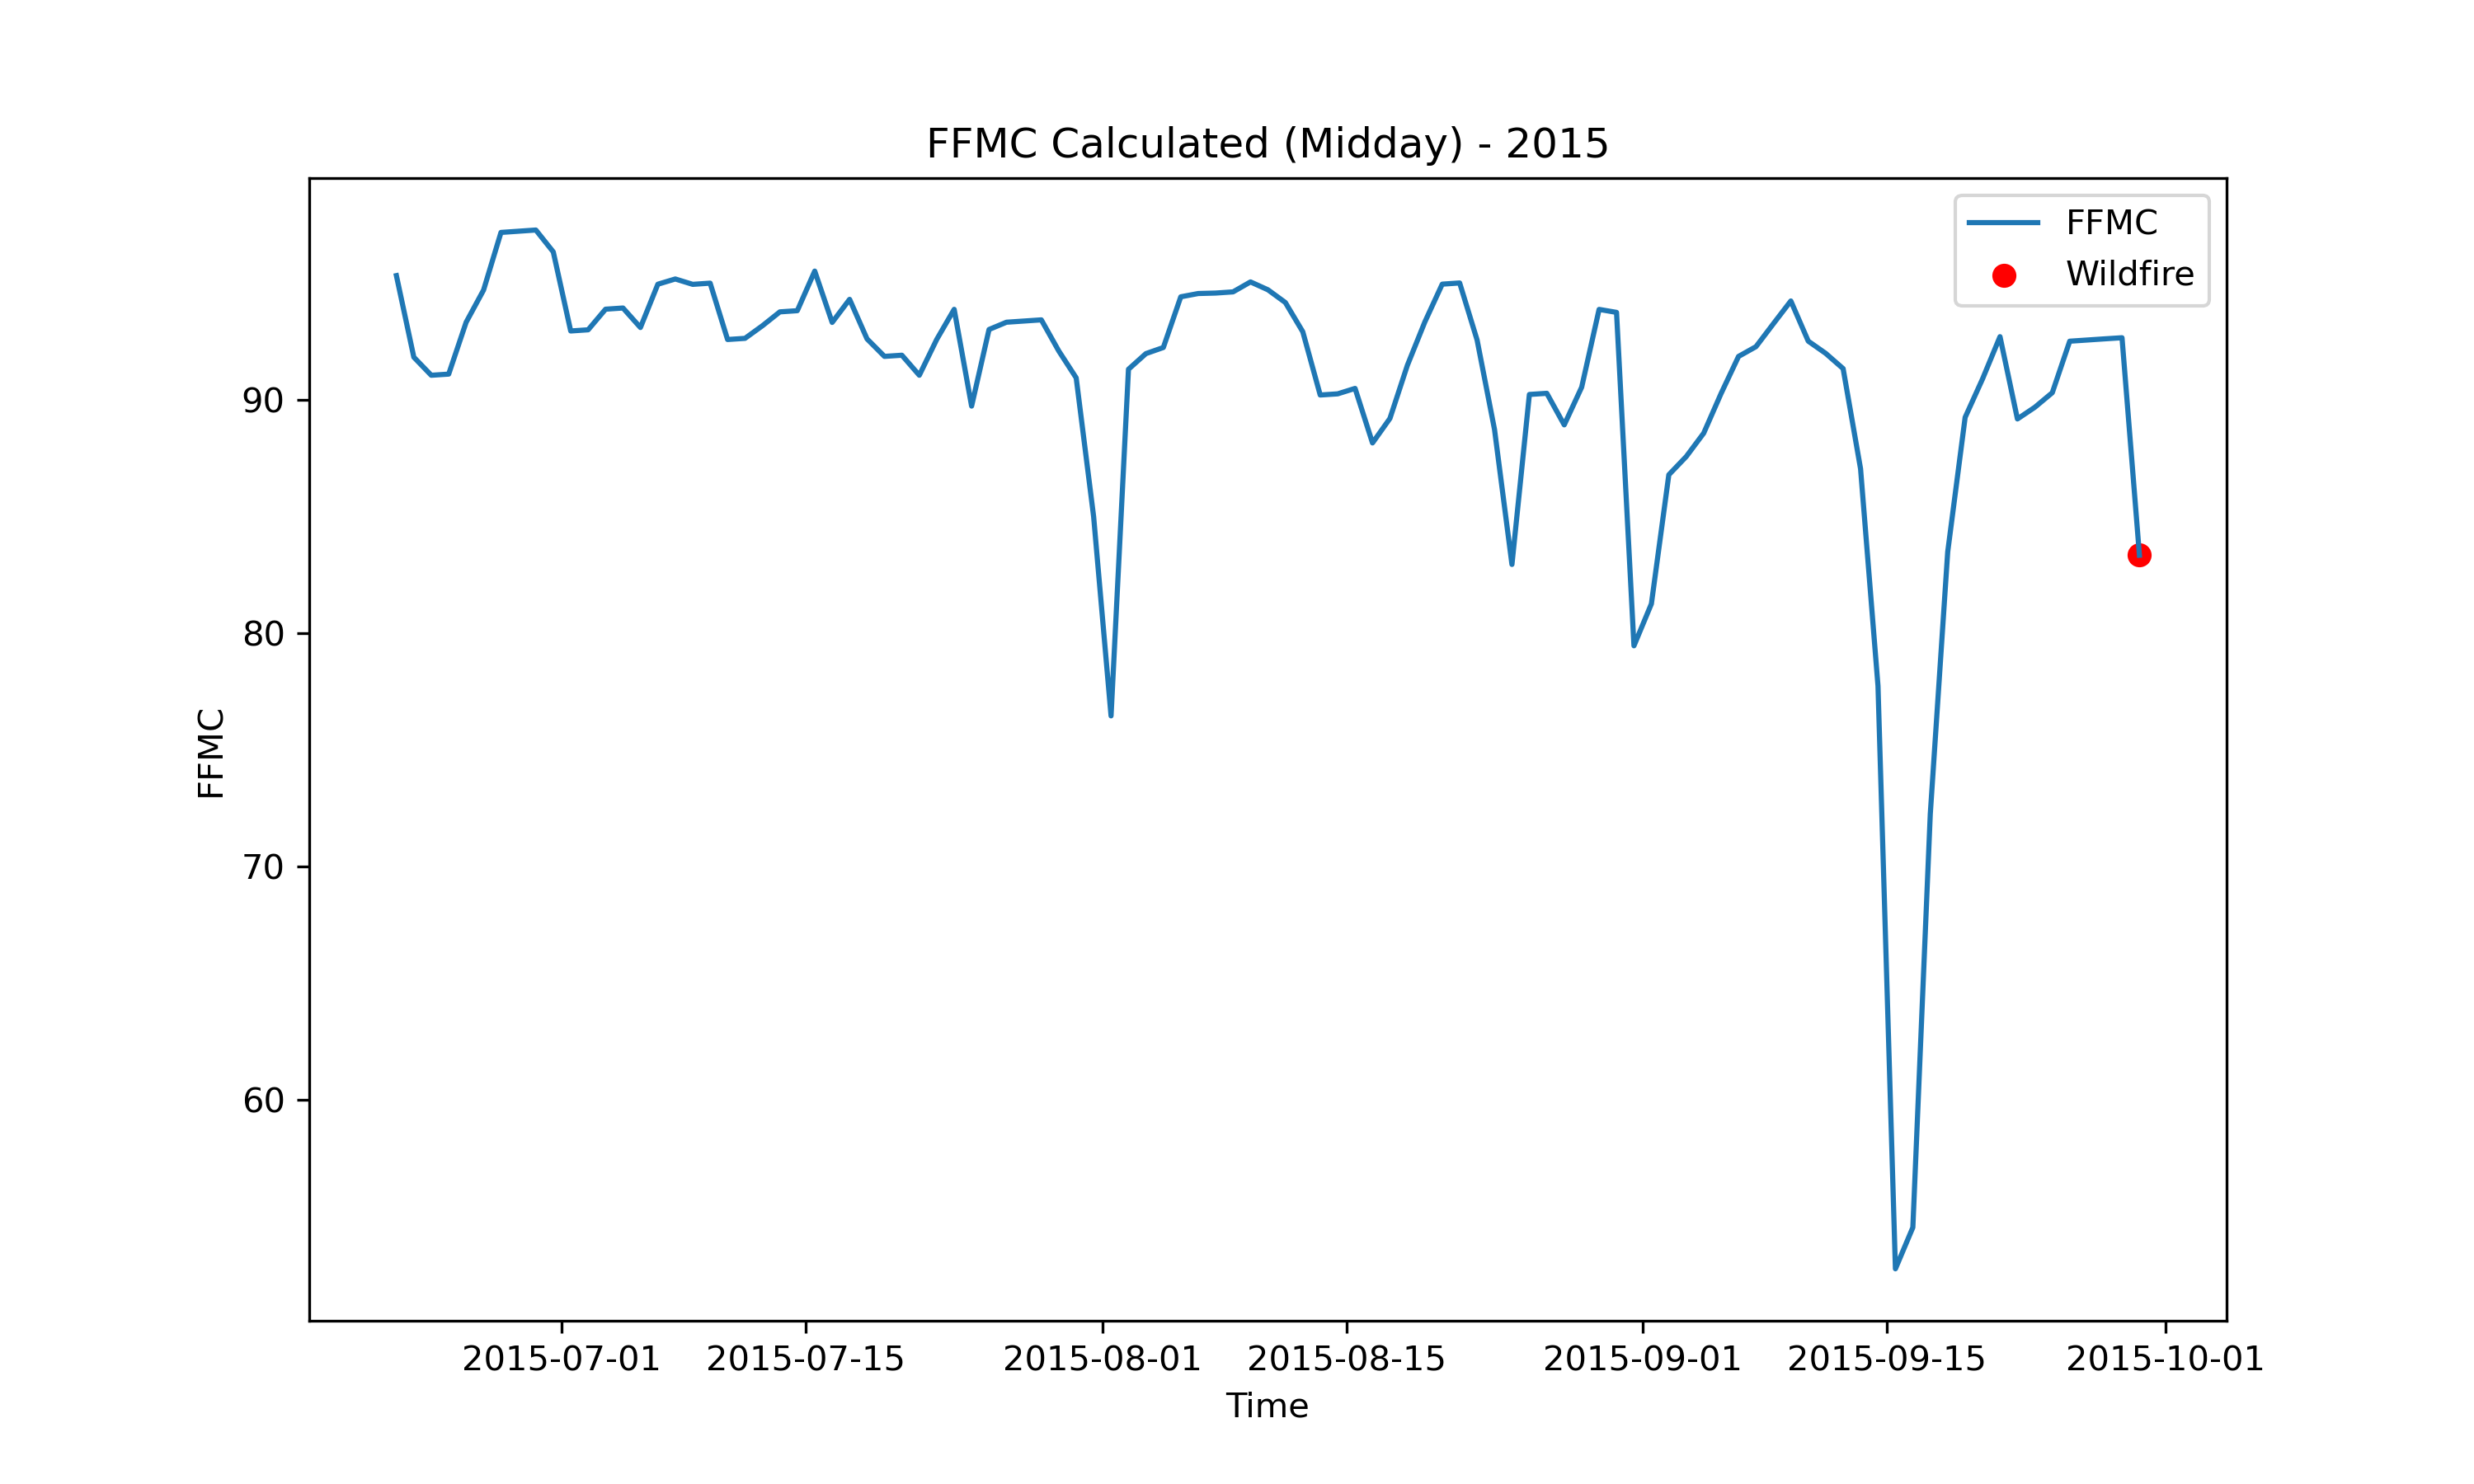
\includegraphics[width=\textwidth]{graphs/2015/2015CalcFFMC12.png}
        \caption{FFMC - Calculated value}
        \label{fig:ffmc_calculated_2015_midday}
    \end{subfigure}
    \label{fig:comparison_ffmc_midday_copernicus_calculated}
\end{figure}

\begin{figure}[h]
\caption{Comparison of DMC calculated values and Copernicus at midday}
    \centering
    \begin{subfigure}{0.49\textwidth}
        \centering
        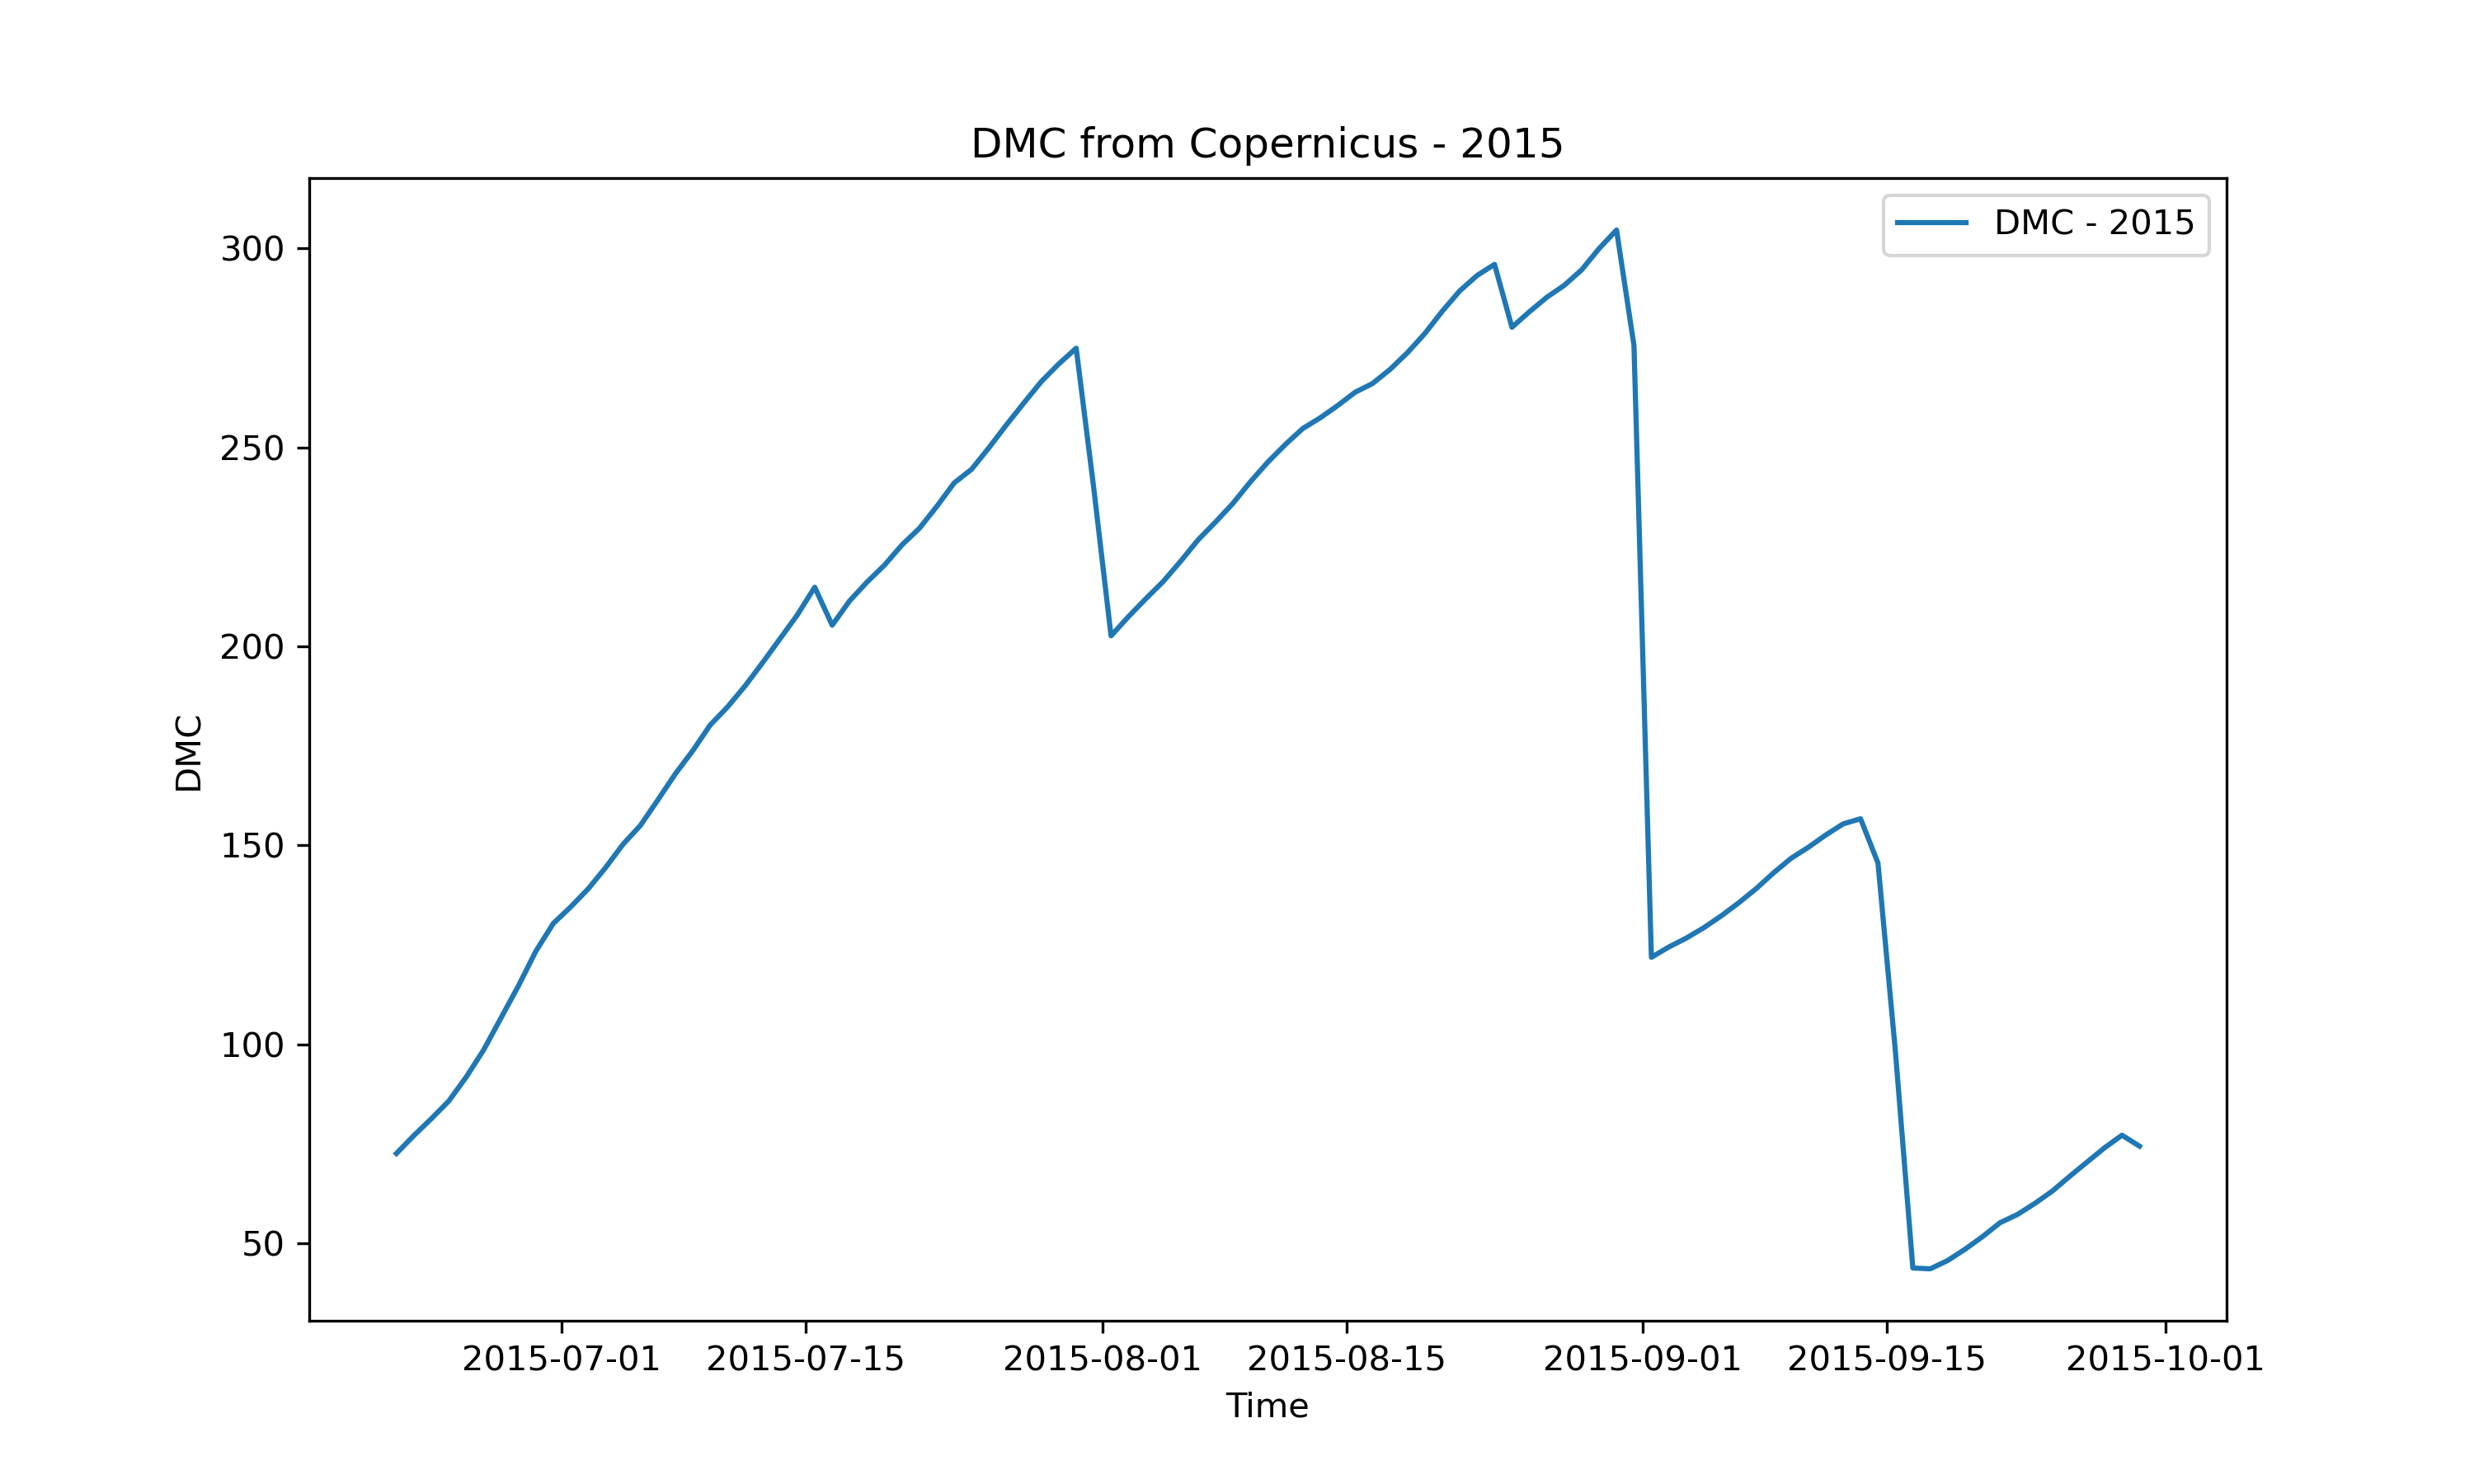
\includegraphics[width=\textwidth]{graphs/2015/2015CopernicusDMC12.png}
        \caption{DMC - Copernicus}
        \label{fig:dmc_copernicus_2015_midday}
    \end{subfigure}
    \hfill
    \begin{subfigure}{0.49\textwidth}
        \centering
        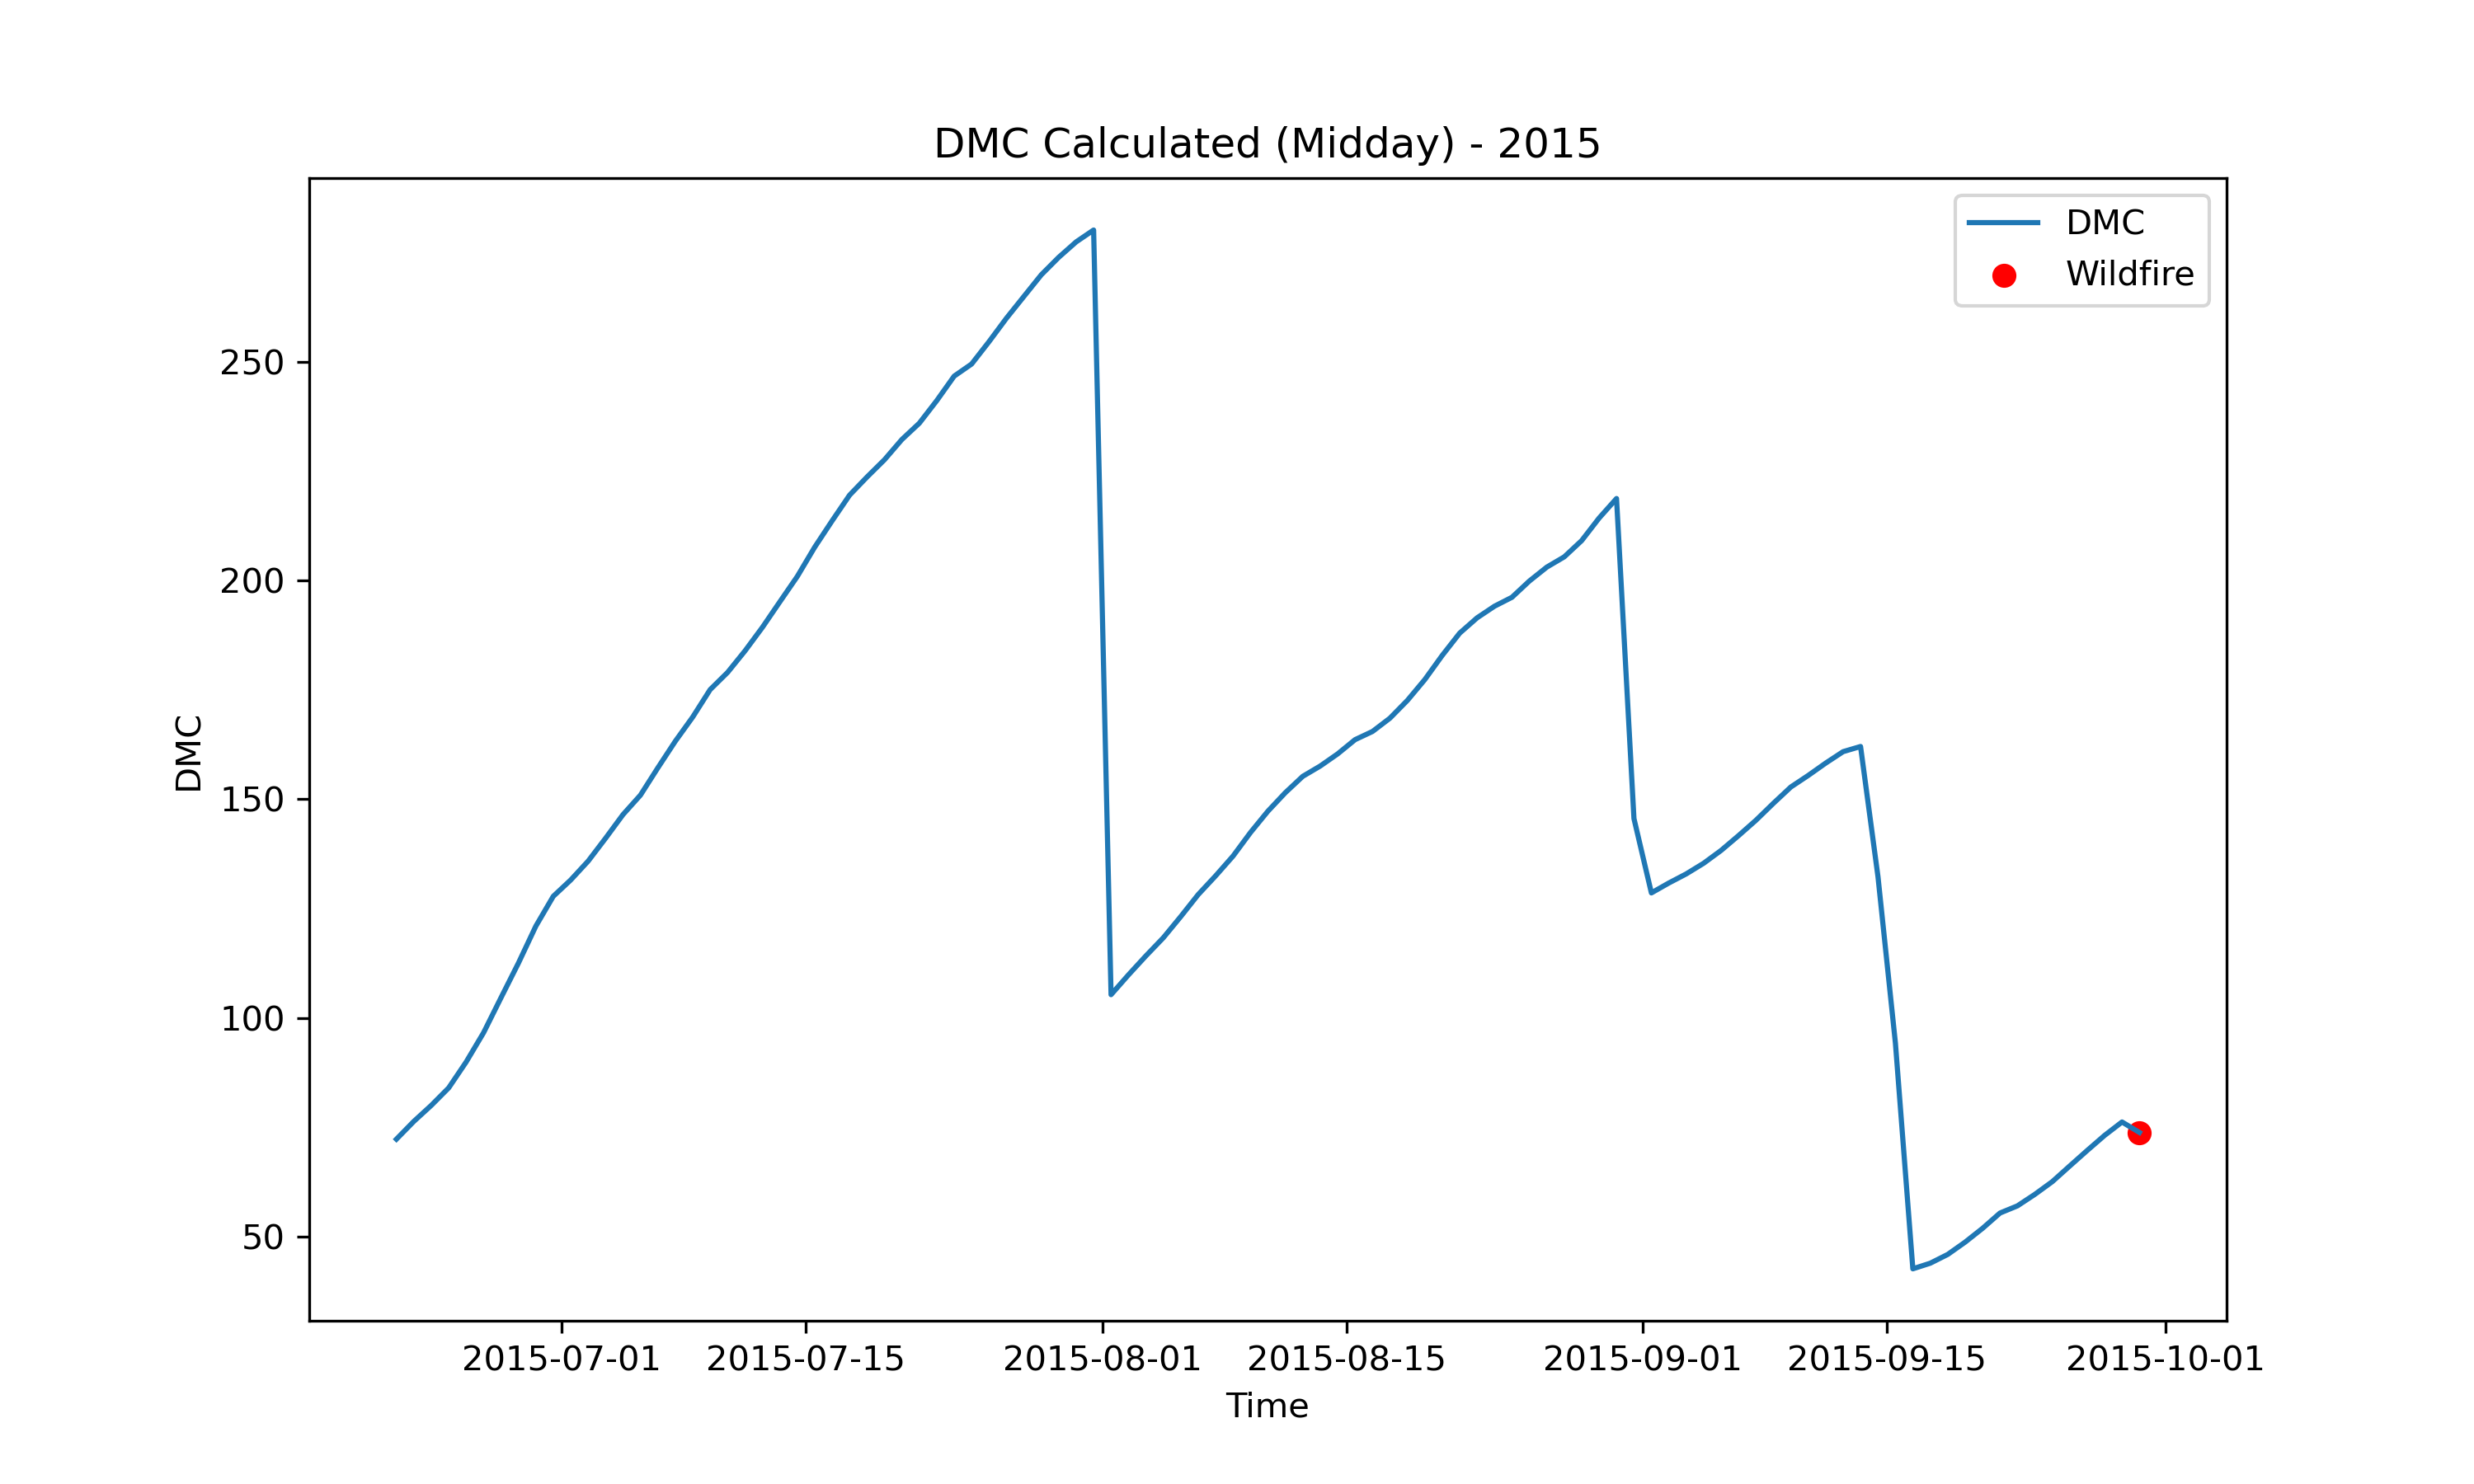
\includegraphics[width=\textwidth]{graphs/2015/2015CalcDMC12.png}
        \caption{DMC - Calculated value}
        \label{fig:dmc_calculated_2015_midday}
    \end{subfigure}
    \label{fig:comparison_dmc_midday_copernicus_calculated}
\end{figure}

\begin{figure}[h]
\caption{Comparison of DC calculated values and Copernicus at midday}
    \centering
    \begin{subfigure}{0.49\textwidth}
        \centering
        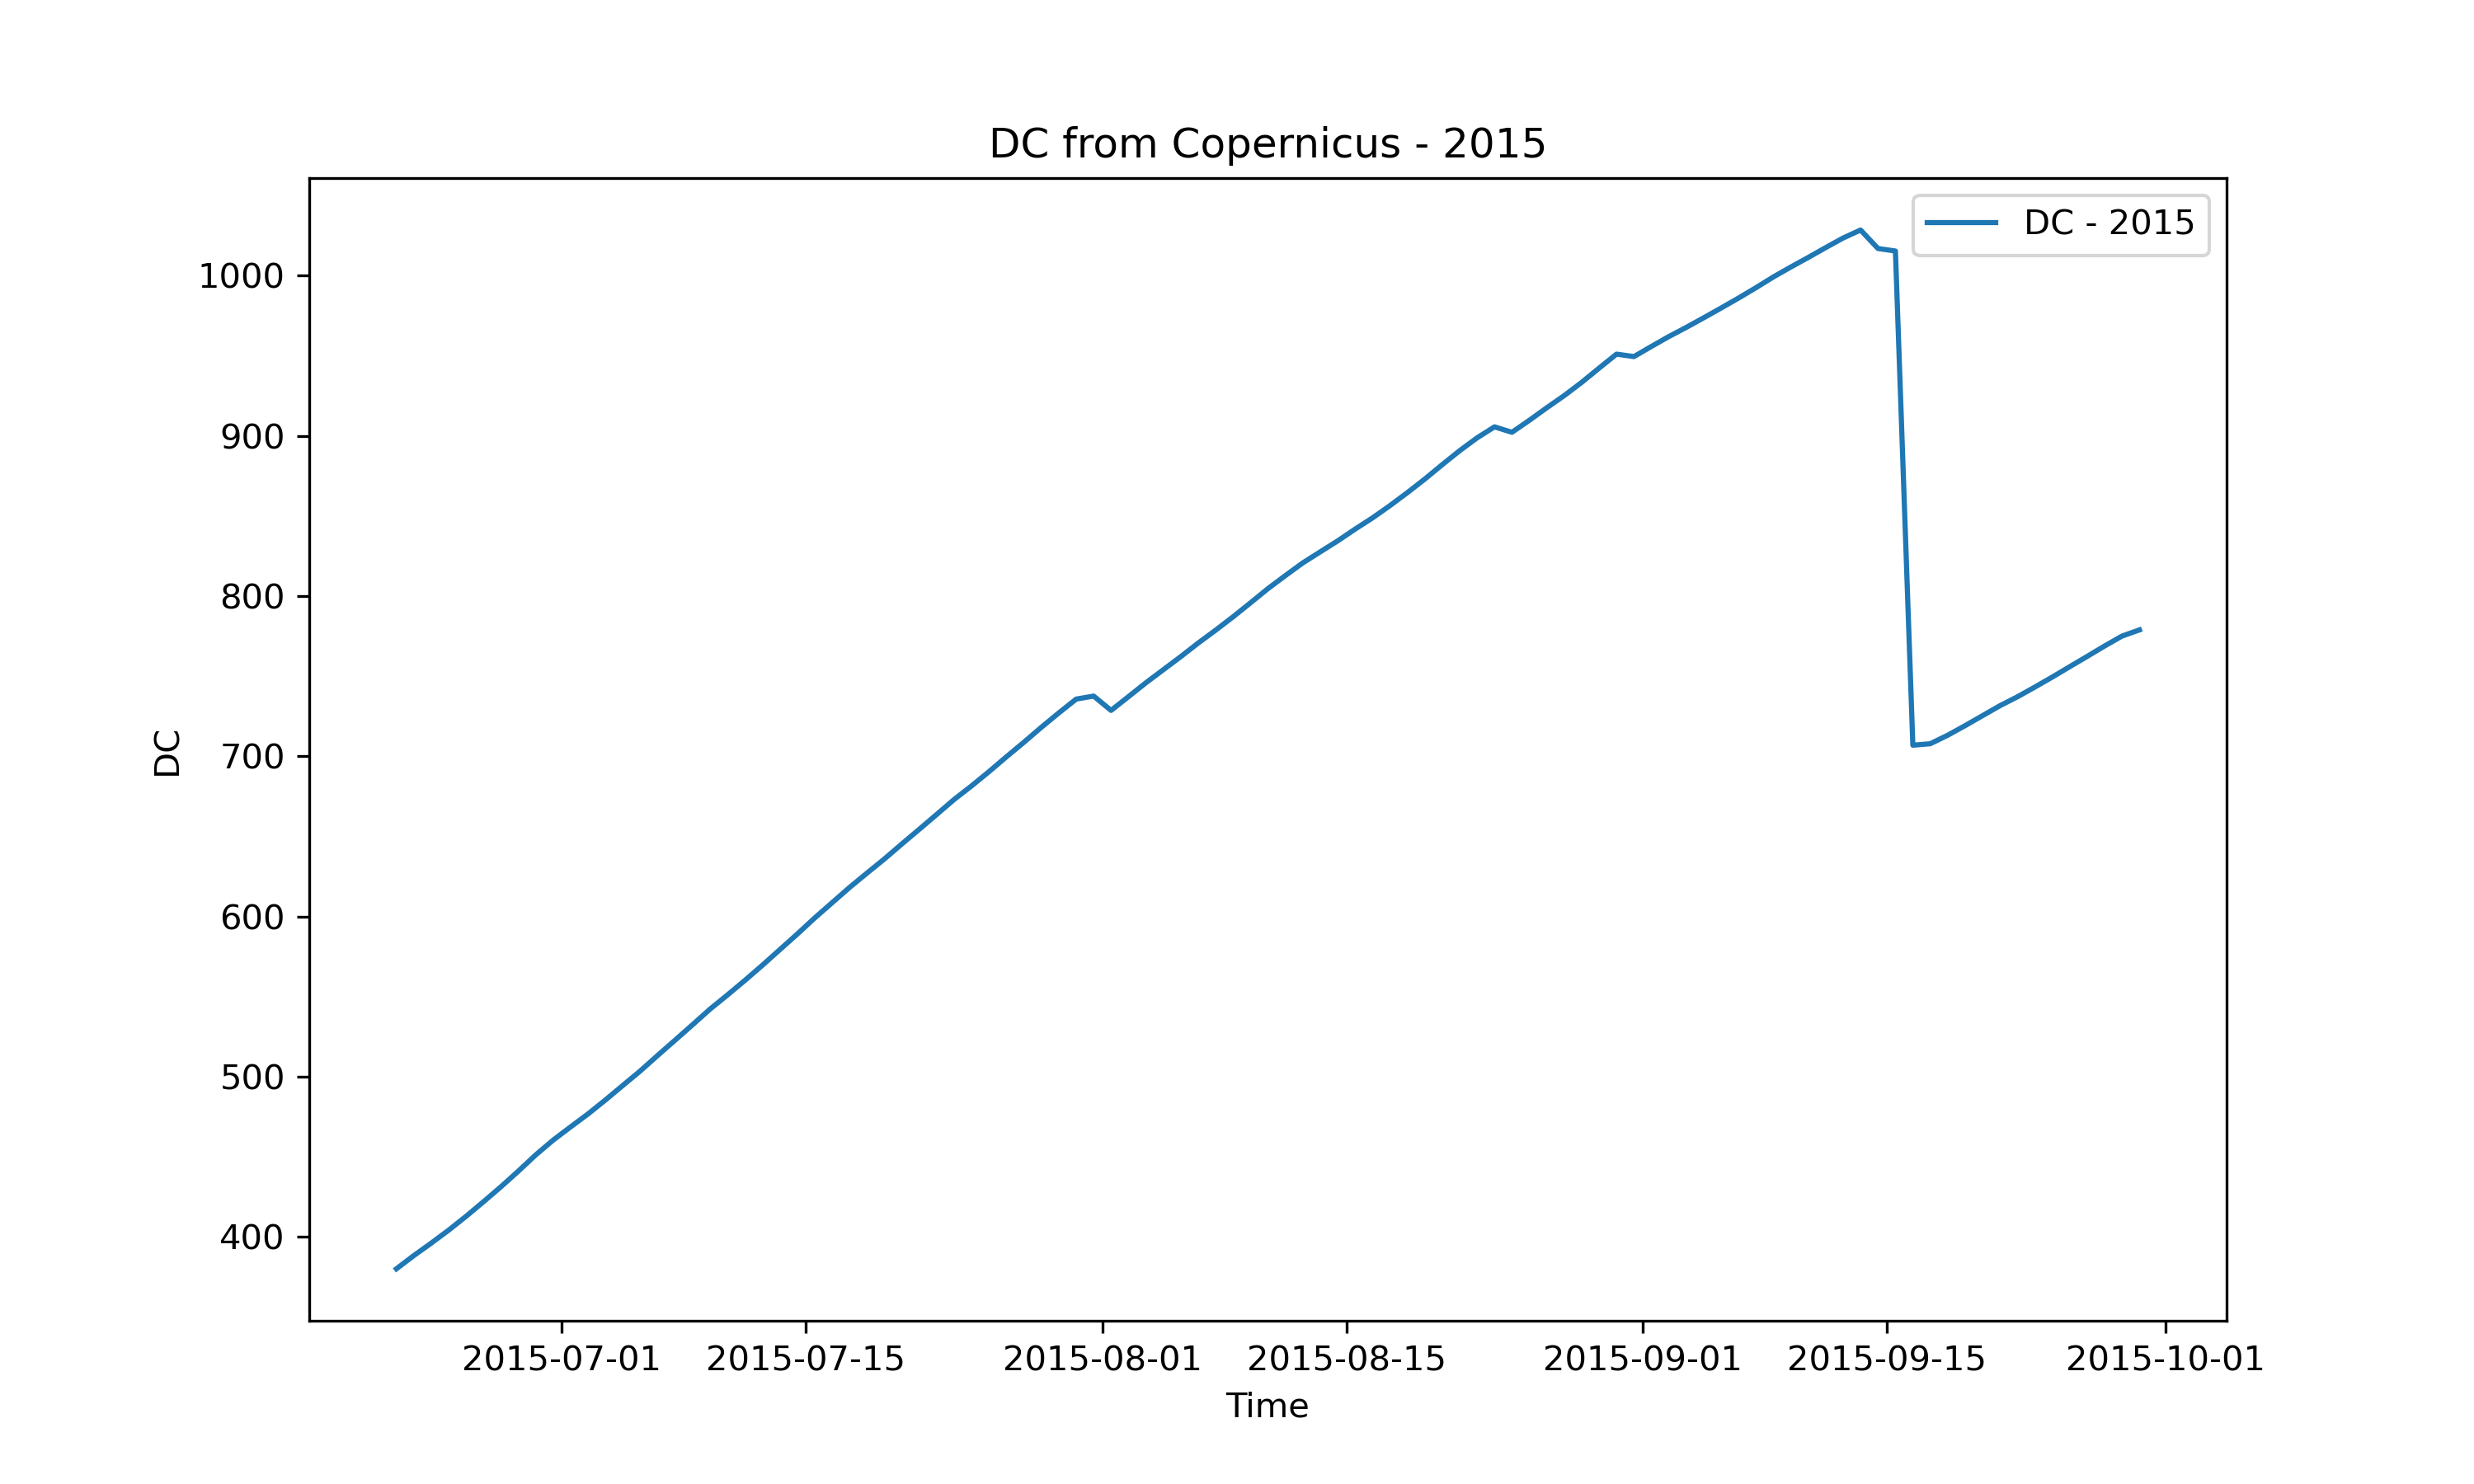
\includegraphics[width=\textwidth]{graphs/2015/2015CopernicusDC12.png}
        \caption{DC - Copernicus}
        \label{fig:dc_copernicus_2015_midday}
    \end{subfigure}
    \hfill
    \begin{subfigure}{0.49\textwidth}
        \centering
        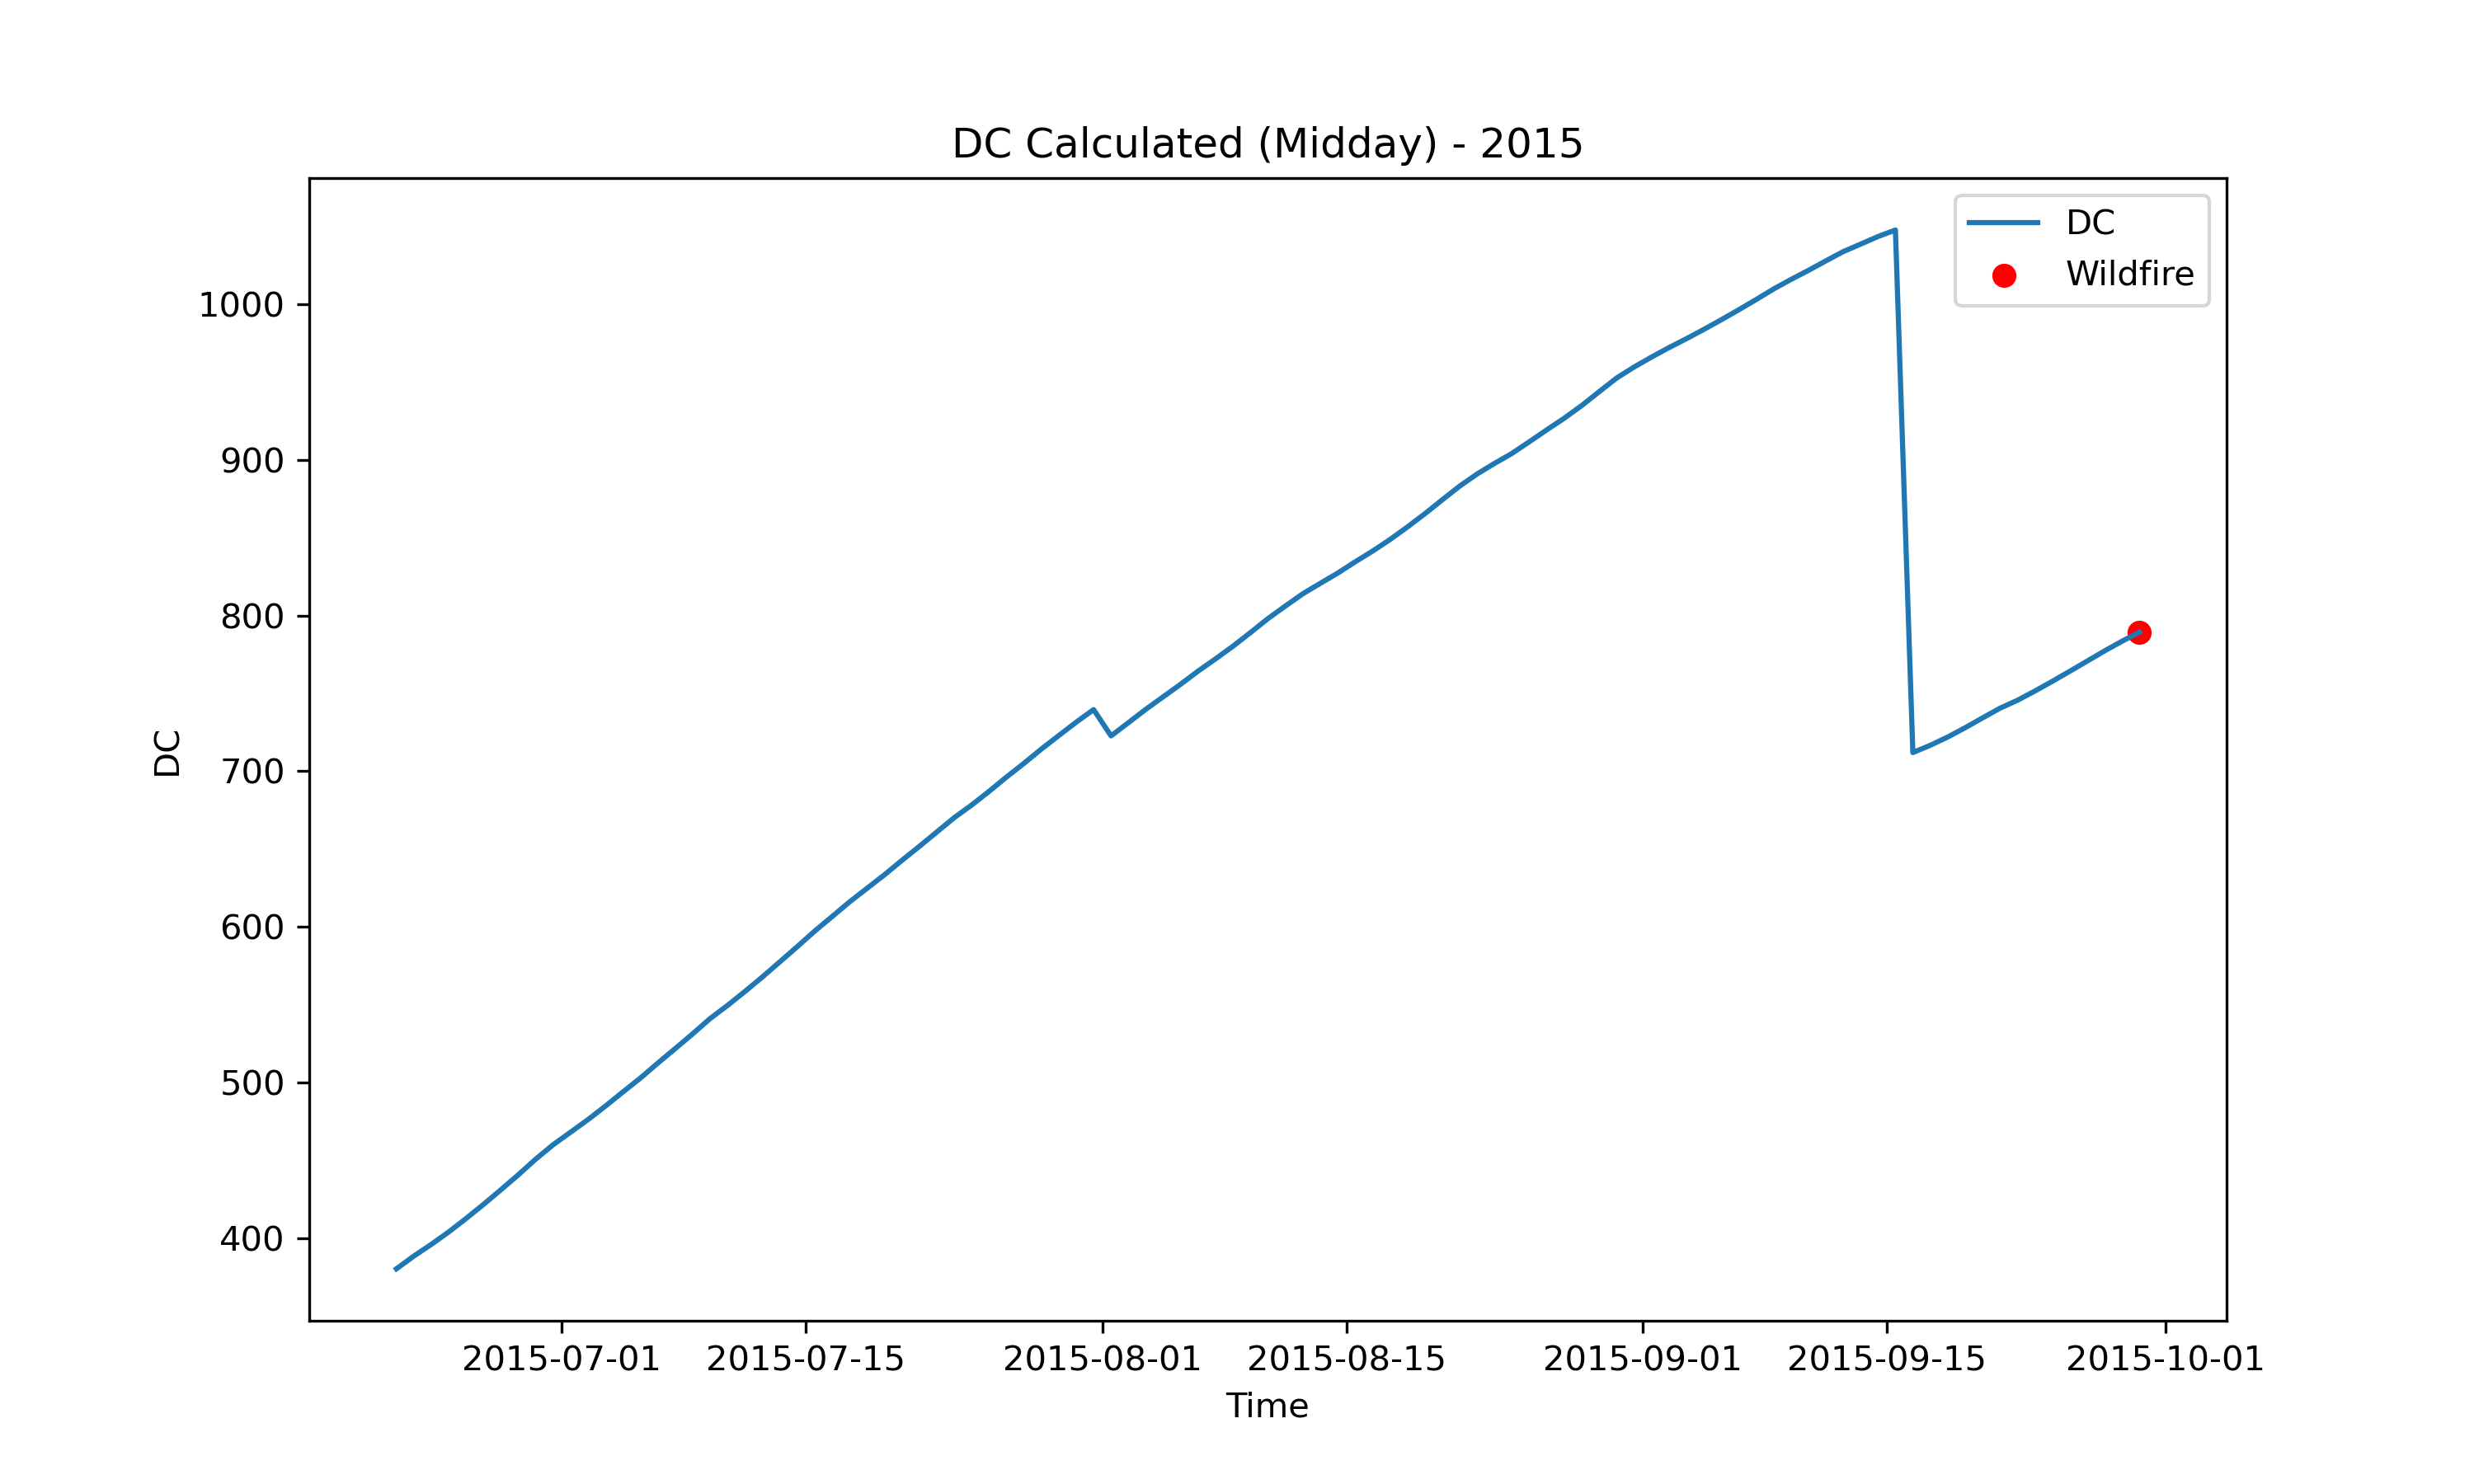
\includegraphics[width=\textwidth]{graphs/2015/2015CalcDC12.png}
        \caption{DC - Calculated value}
        \label{fig:dc_calculated_2015_midday}
    \end{subfigure}
    \label{fig:comparison_dc_midday_copernicus_calculated}
\end{figure}

\begin{figure}[h]
	\caption{Comparison of ISI calculated values and Copernicus at midday}
	\centering
	\begin{subfigure}{0.49\textwidth}
		\centering
		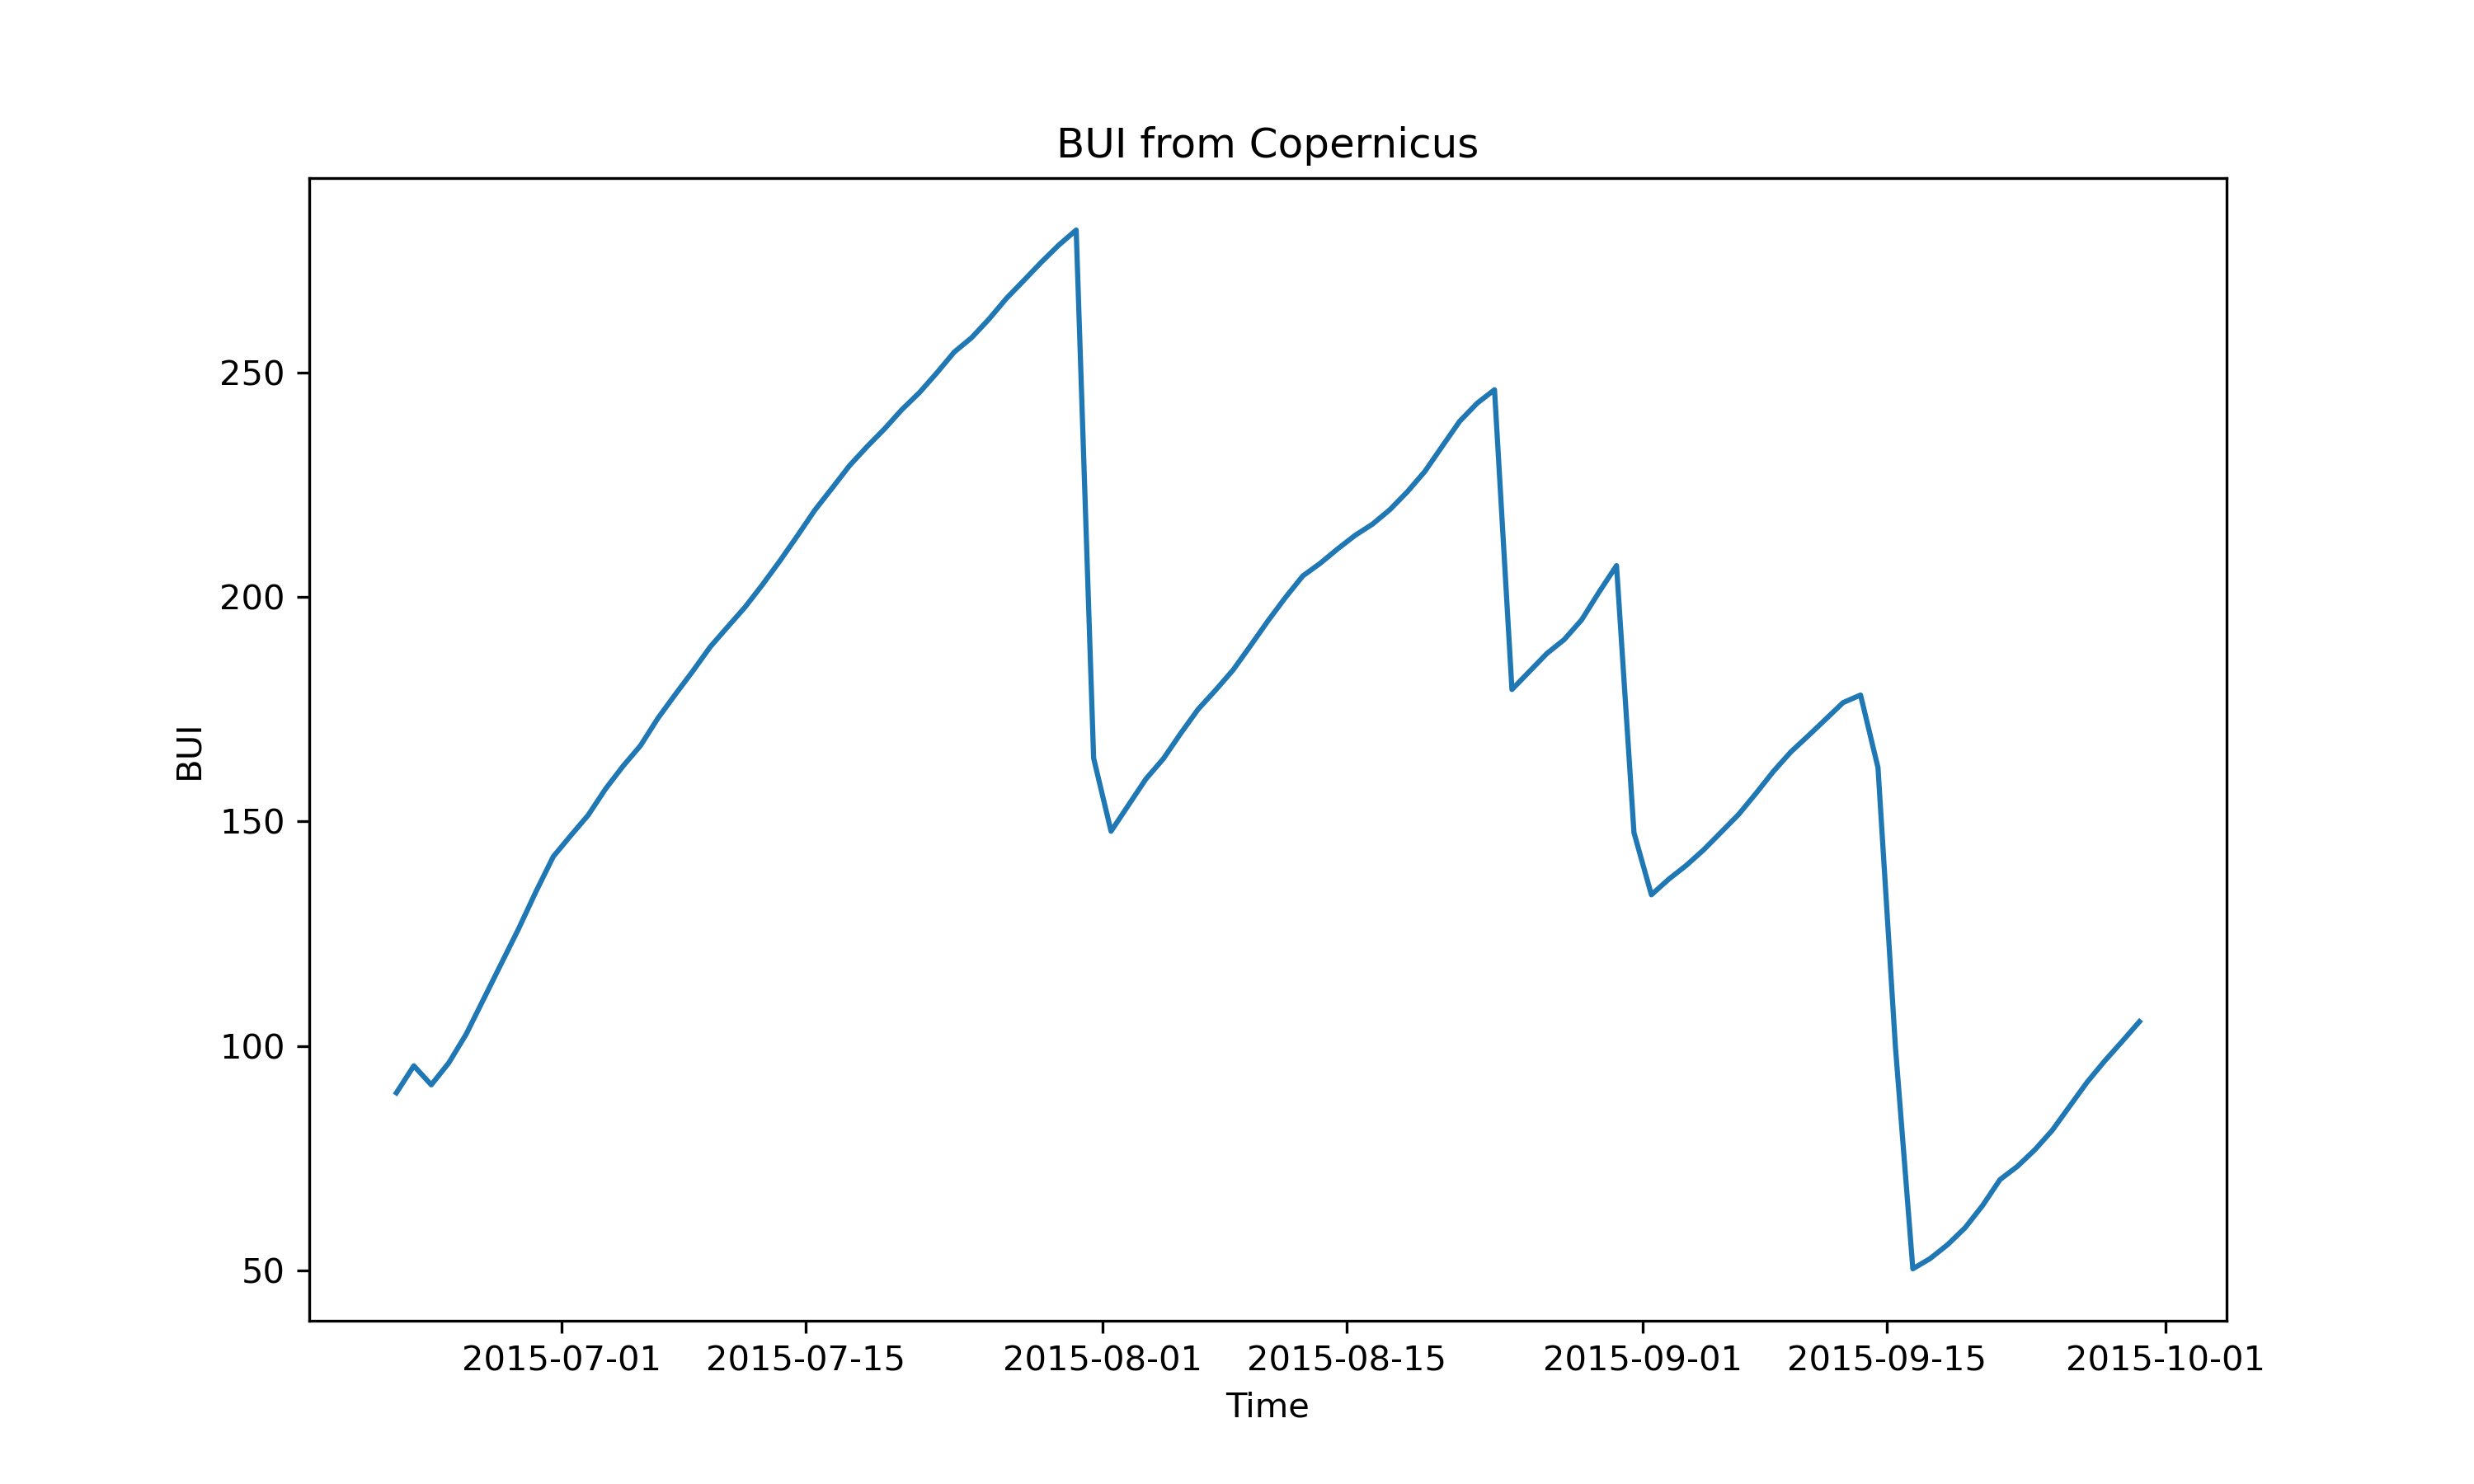
\includegraphics[width=\textwidth]{graphs/2015/2015CopernicusISI12.png}
		\caption{ISI - Copernicus}
		\label{fig:isi_copernicus_2015_midday}
	\end{subfigure}
	\hfill
	\begin{subfigure}{0.49\textwidth}
		\centering
		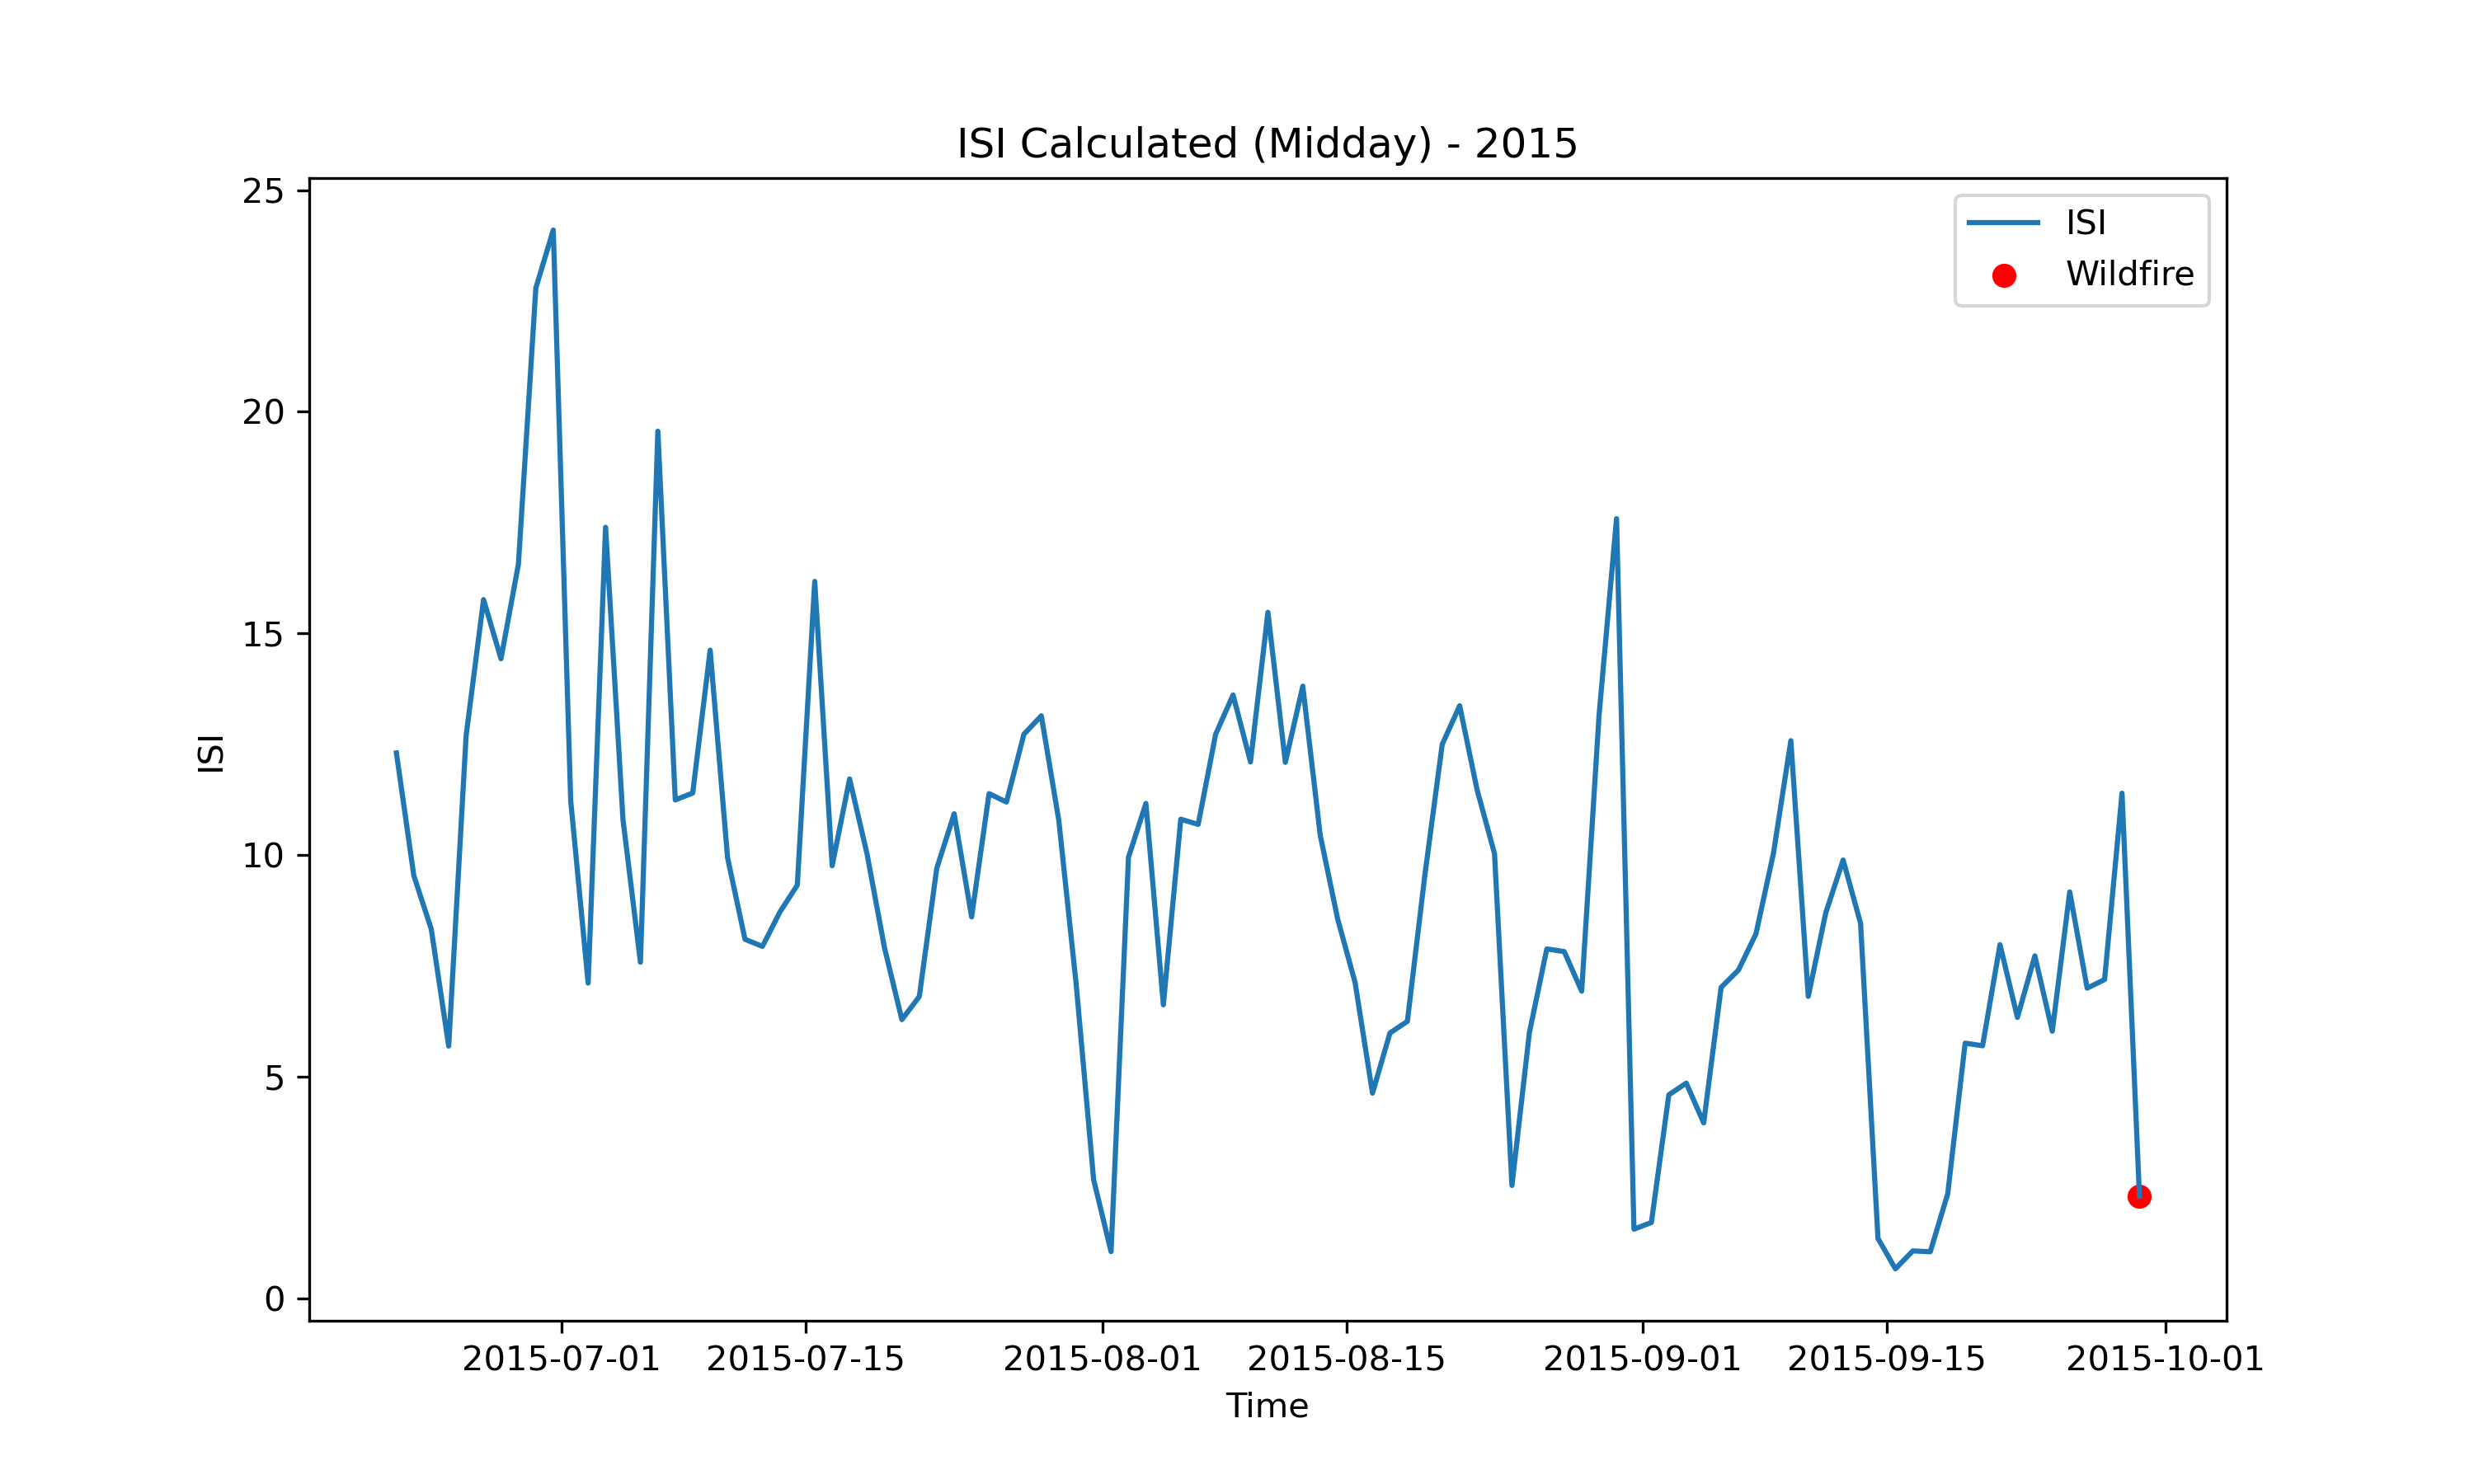
\includegraphics[width=\textwidth]{graphs/2015/2015CalcISI12.png}
		\caption{ISI - Calculated value}
		\label{fig:isi_calculated_2015_midday}
	\end{subfigure}
	\label{fig:comparison_isi_midday_copernicus_calculated}
\end{figure}

\begin{figure}[h]
	\caption{Comparison of BUI calculated values and Copernicus at midday}
	\centering
	\begin{subfigure}{0.49\textwidth}
		\centering
		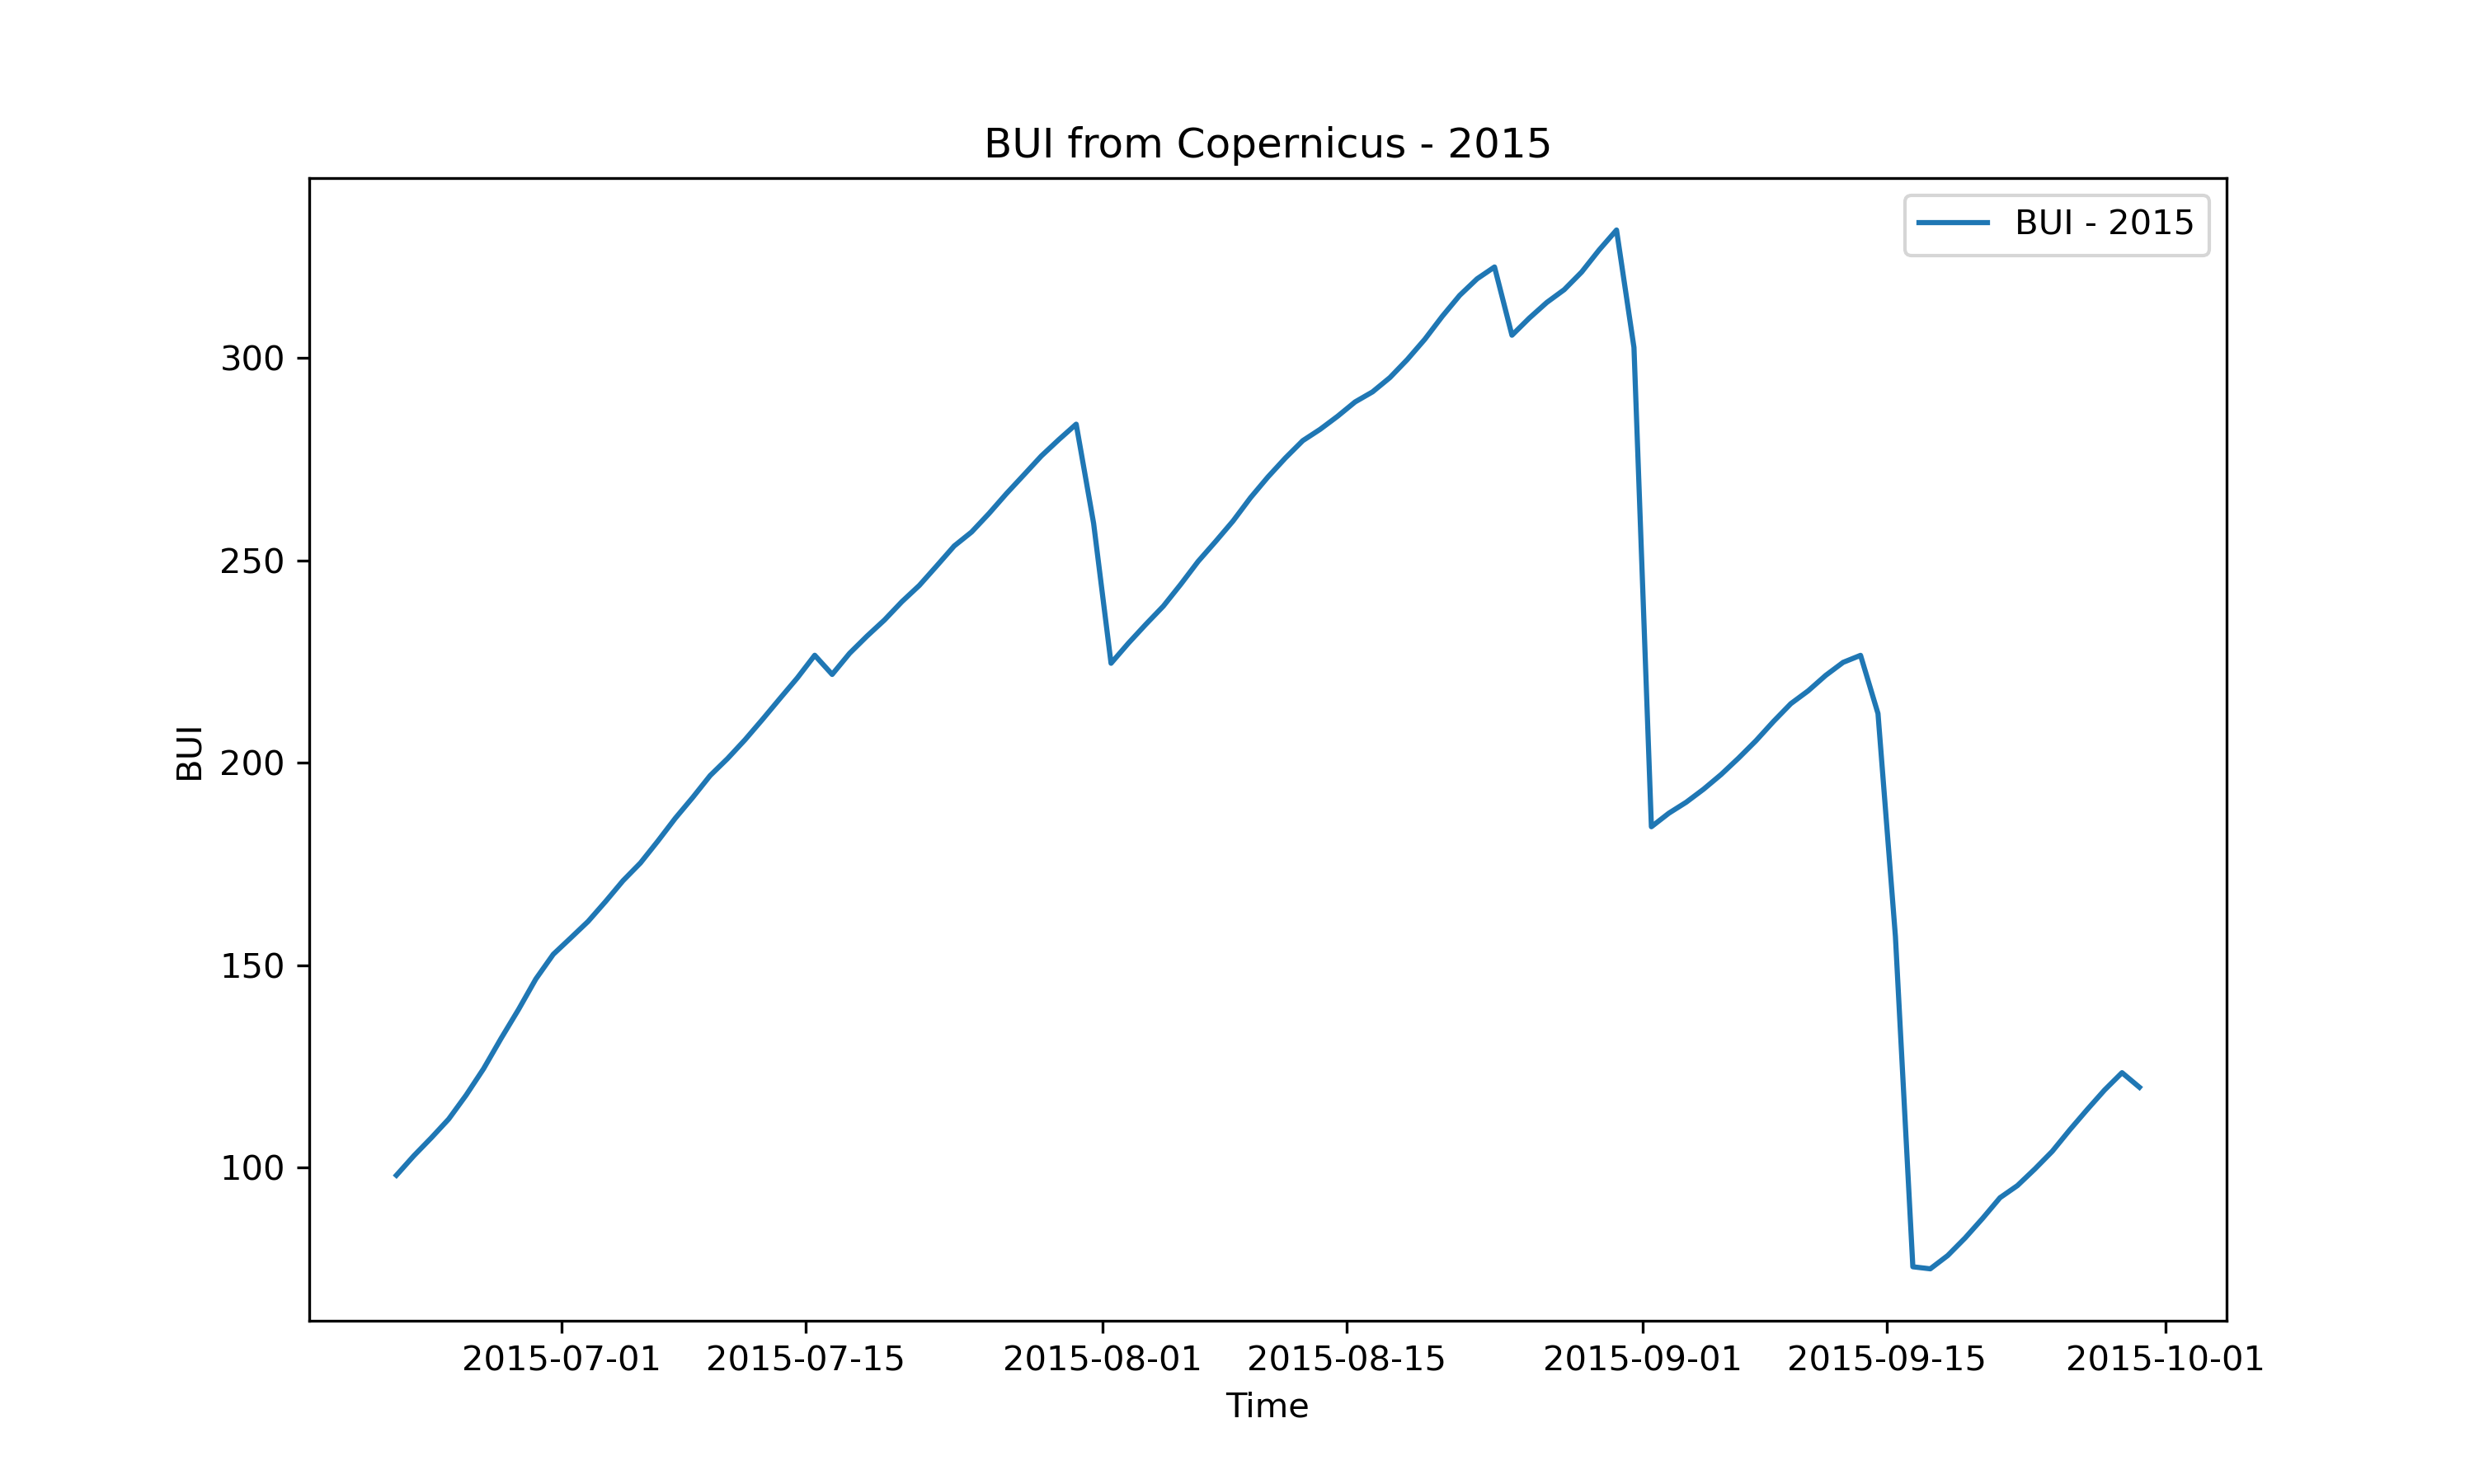
\includegraphics[width=\textwidth]{graphs/2015/2015CopernicusBUI12.png}
		\caption{BUI - Copernicus}
		\label{fig:bui_copernicus_2015_midday}
	\end{subfigure}
	\hfill
	\begin{subfigure}{0.49\textwidth}
		\centering
		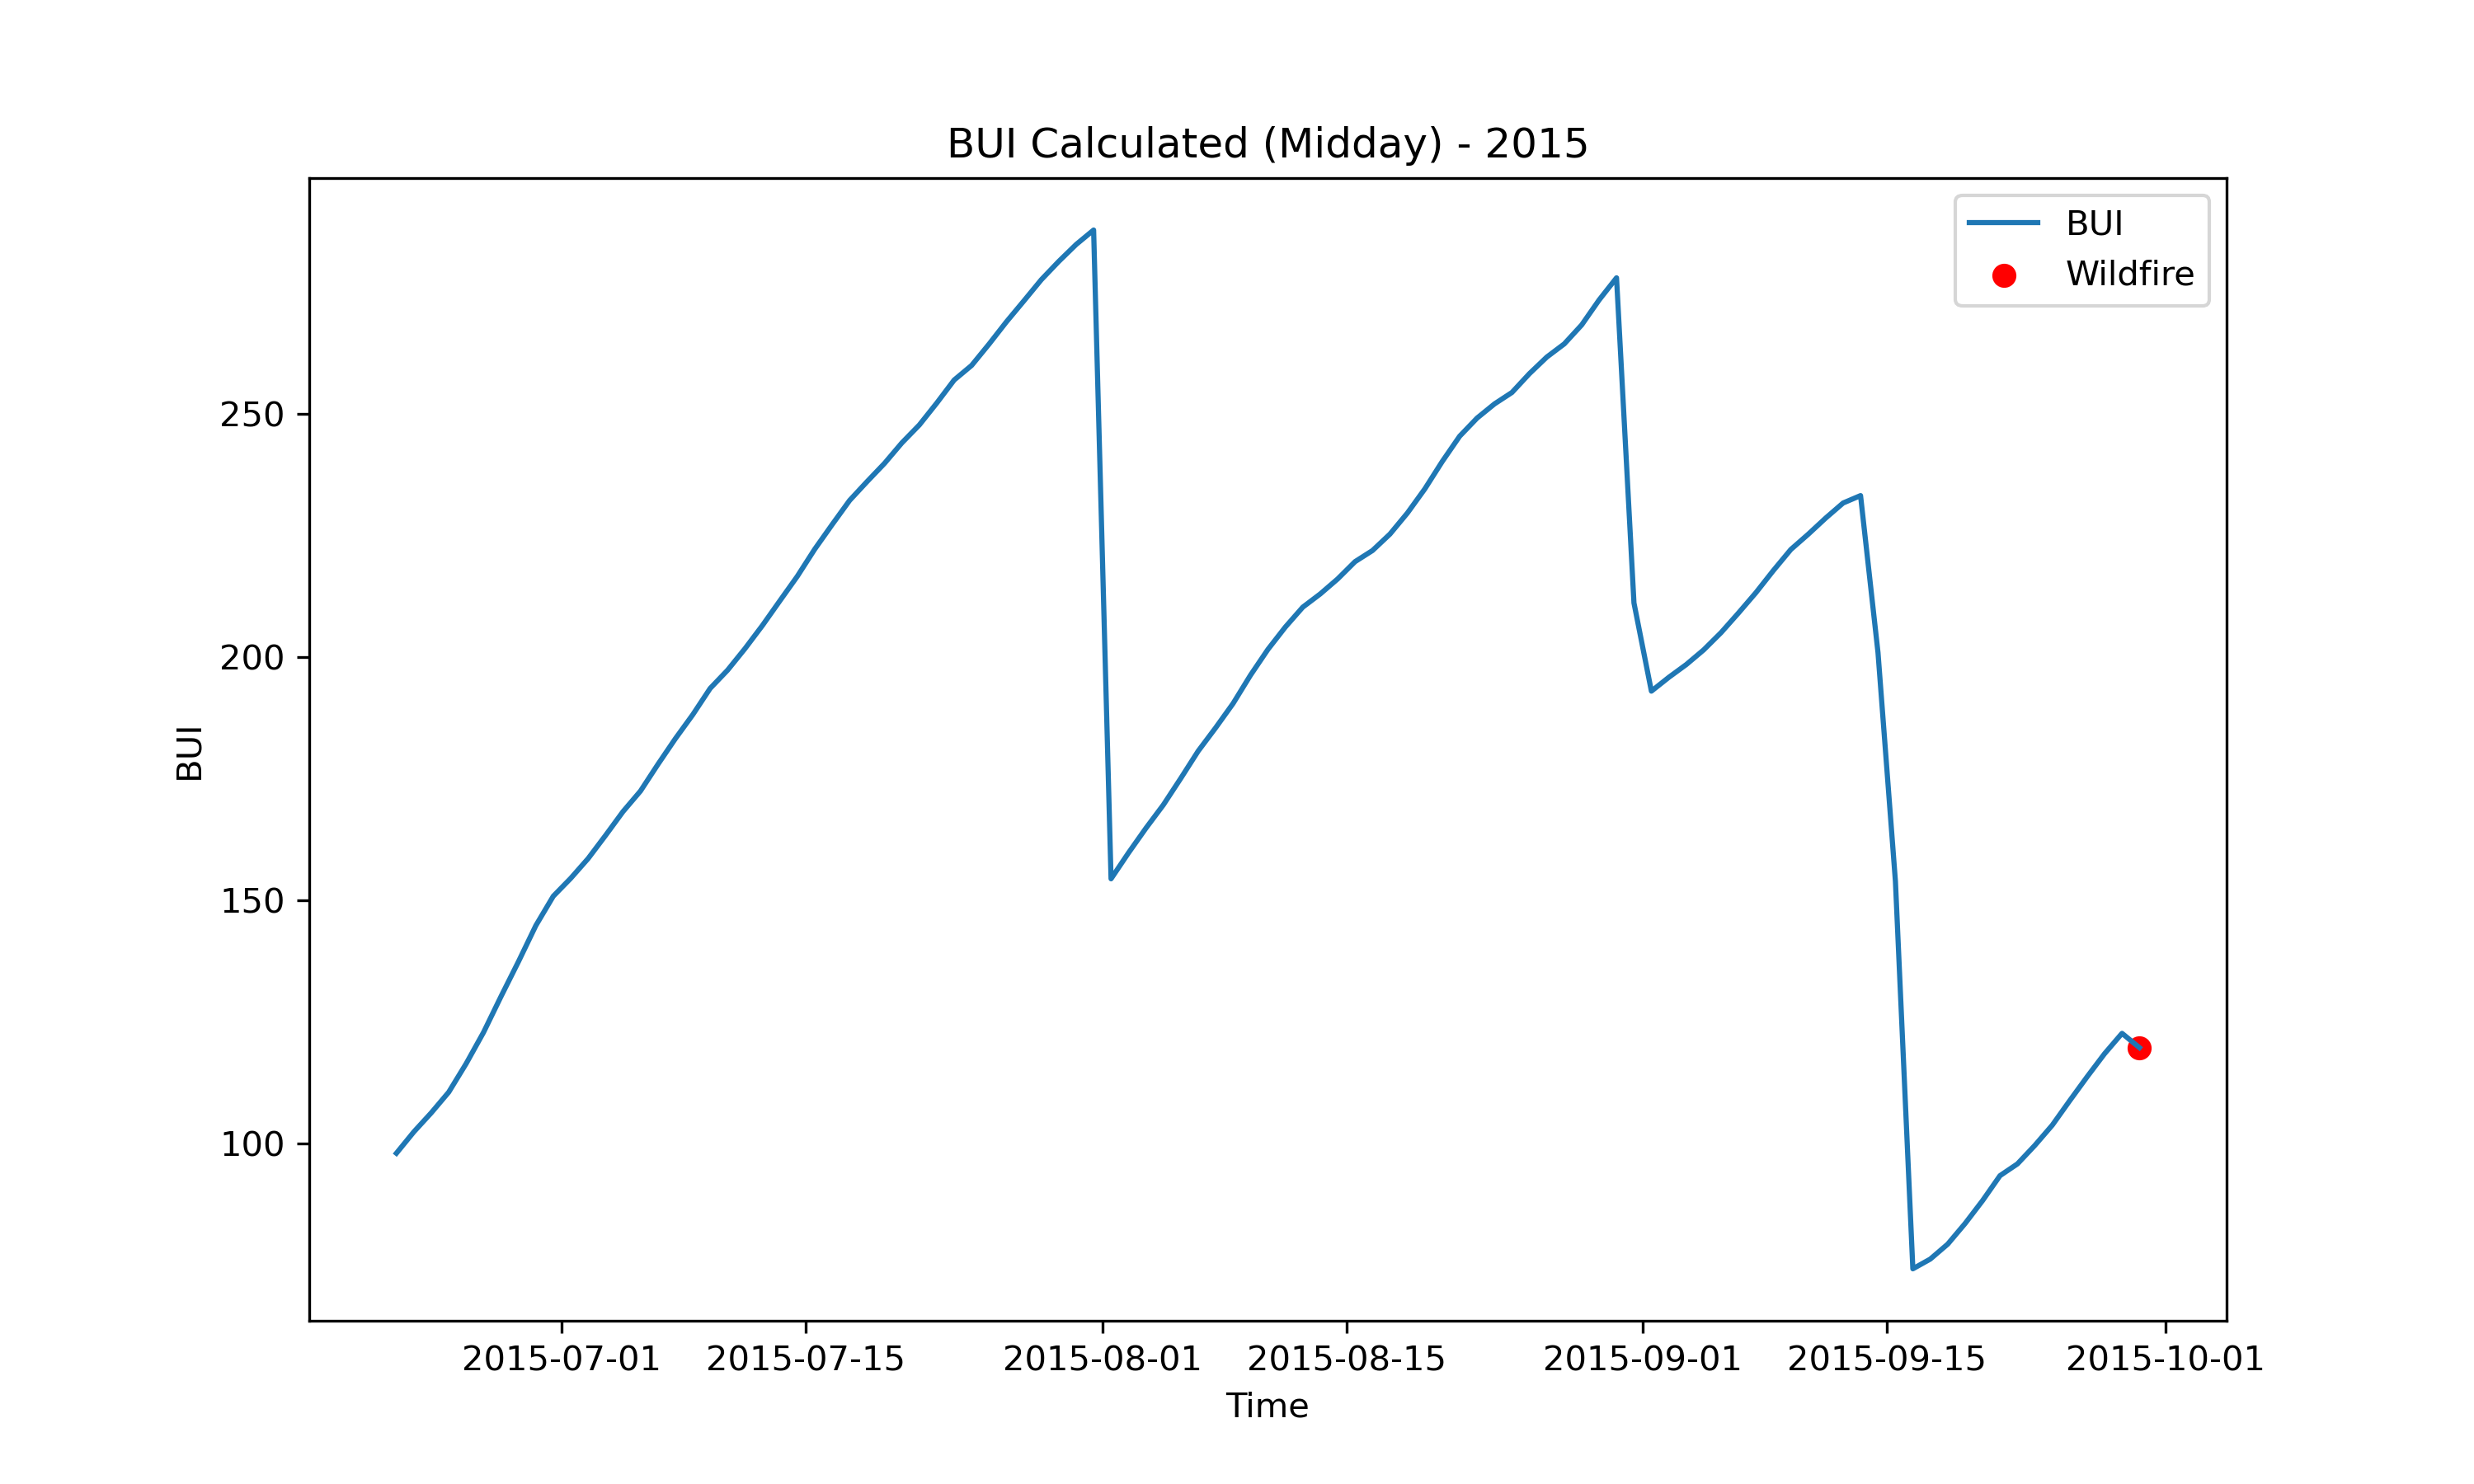
\includegraphics[width=\textwidth]{graphs/2015/2015CalcBUI12.png}
		\caption{BUI - Calculated value}
		\label{fig:bui_calculated_2015_midday}
	\end{subfigure}
	\label{fig:comparison_bui_midday_copernicus_calculated}
\end{figure}

\FloatBarrier

\subsection{Fogo de 2019}


\begin{figure}[h]
	\caption{Comparison of FWI calculated values and Copernicus at midday - 2019}
	\centering
	\begin{subfigure}{0.49\textwidth}
		\centering
		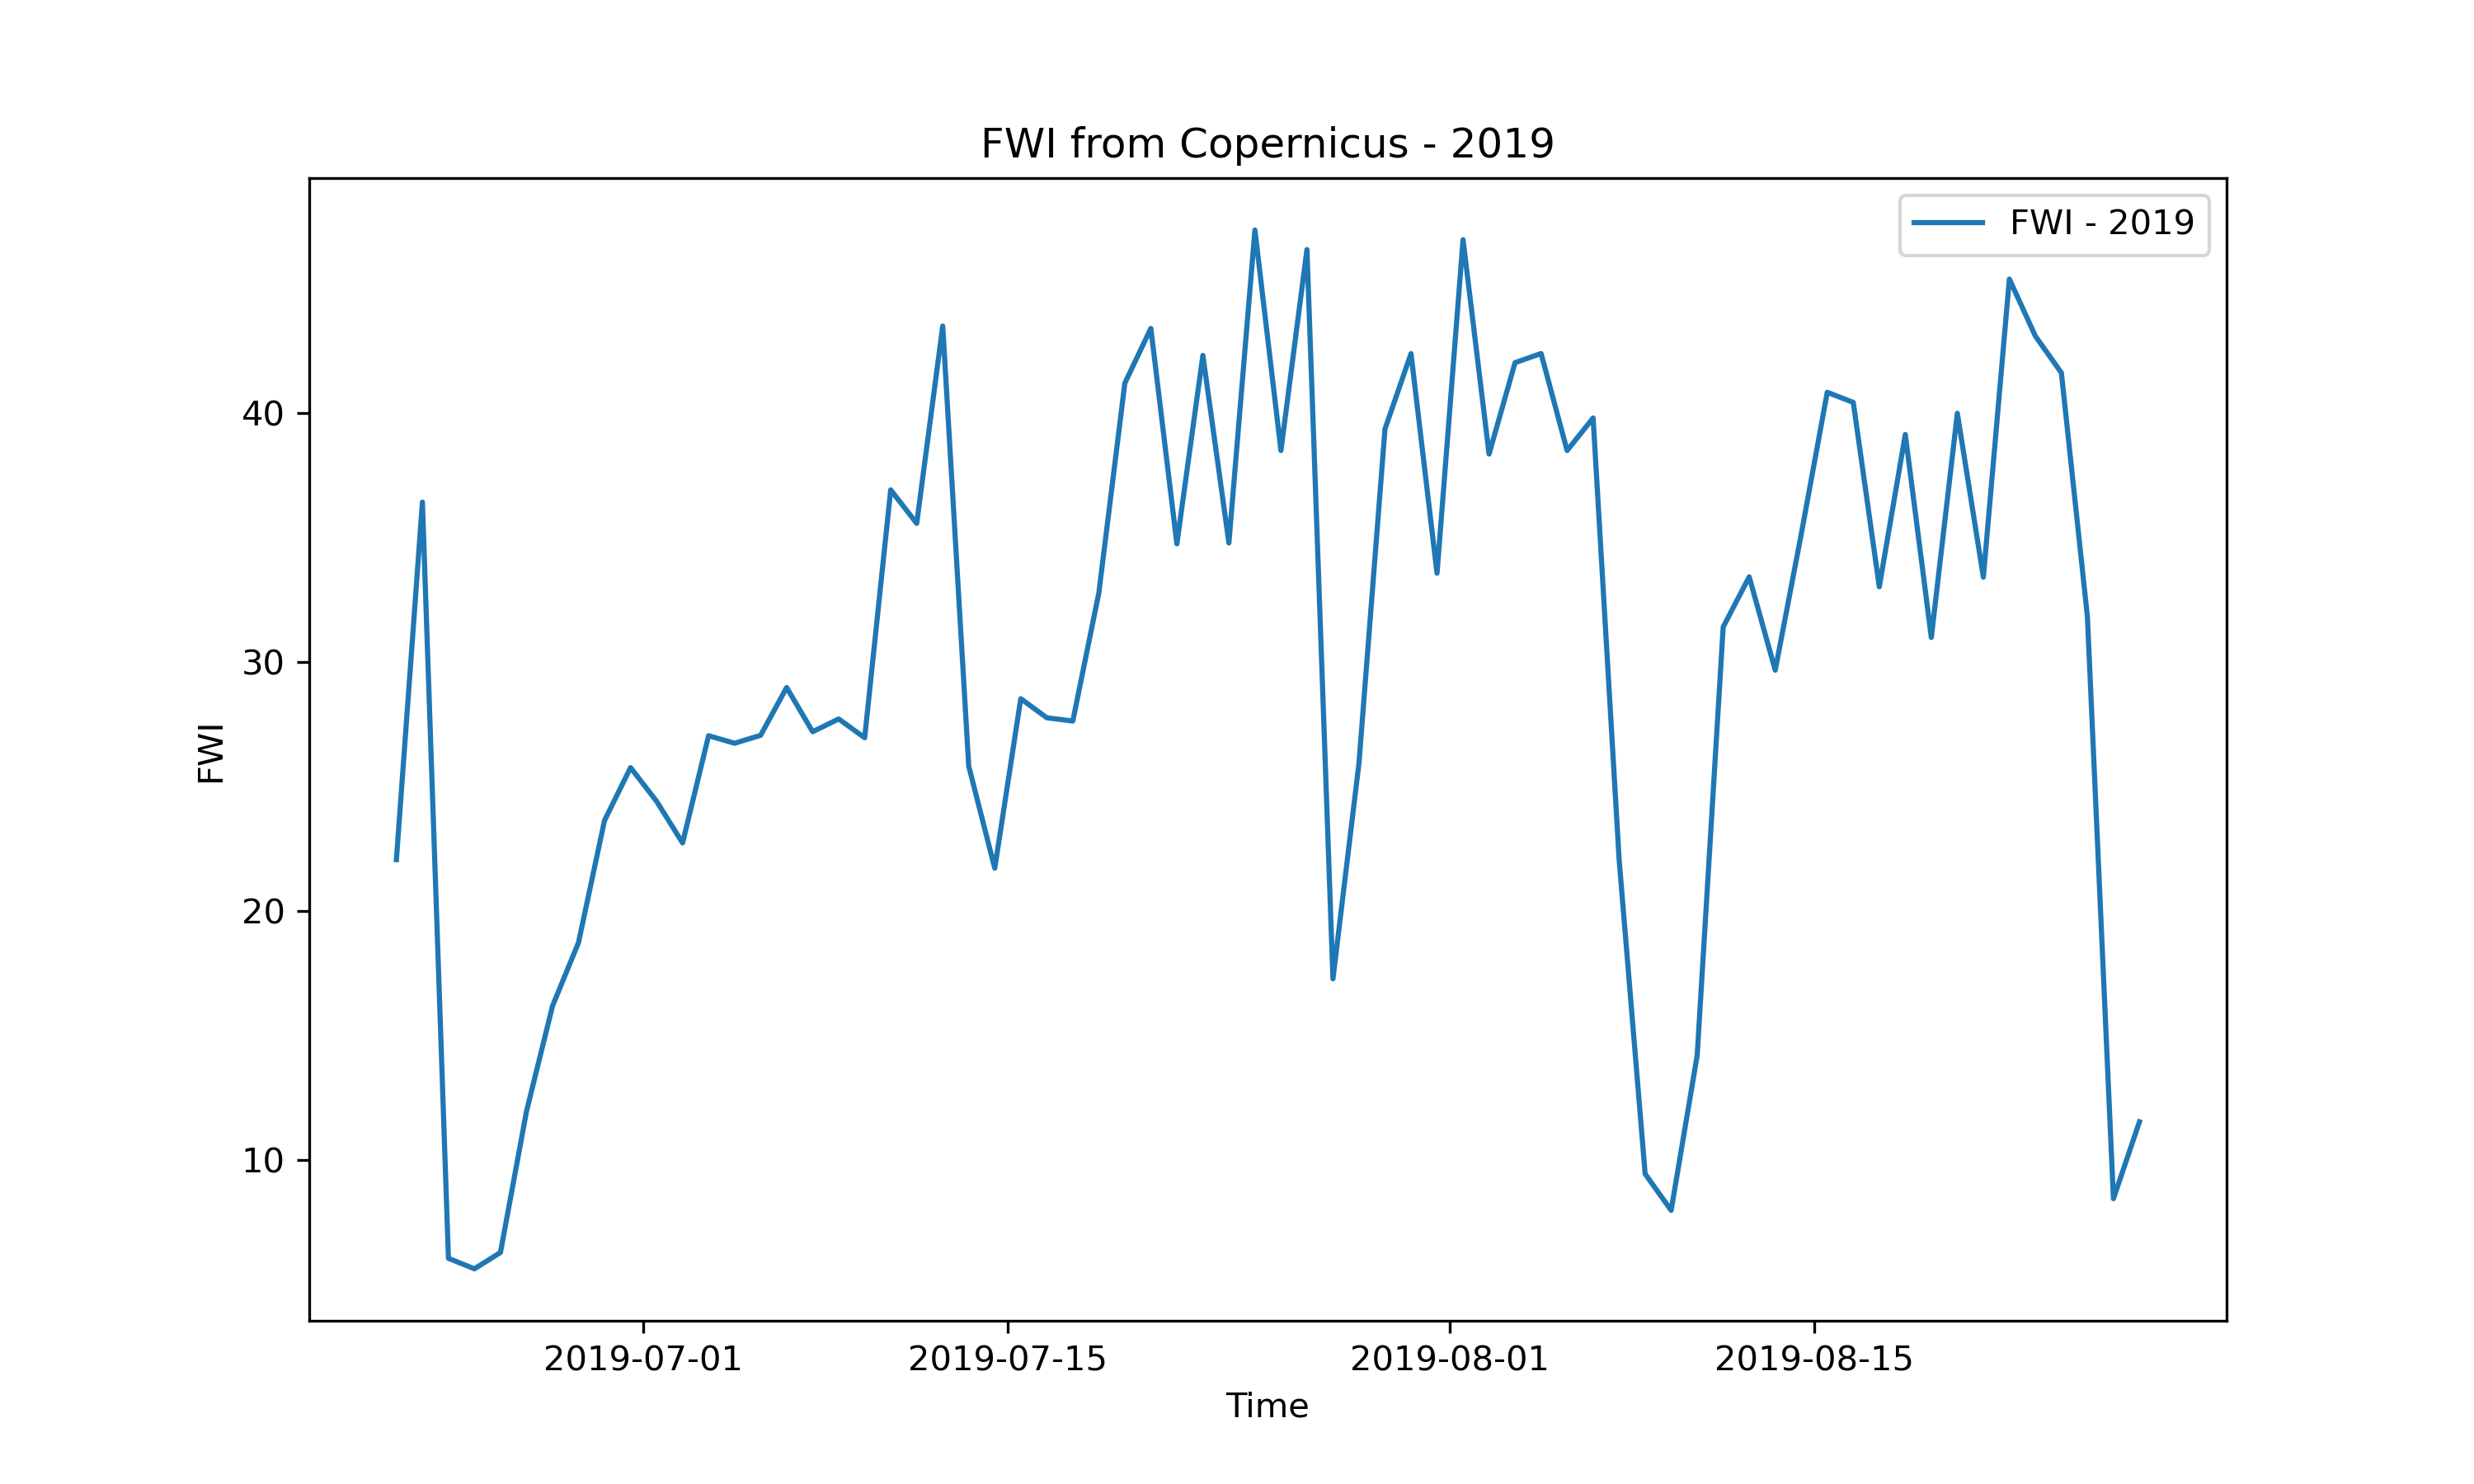
\includegraphics[width=\textwidth]{graphs/2019/2019CopernicusFWI12.png}
		\caption{FWI - Copernicus}
		\label{fig:fwi_copernicus_2019_midday}
	\end{subfigure}
	\hfill
	\begin{subfigure}{0.49\textwidth}
		\centering
		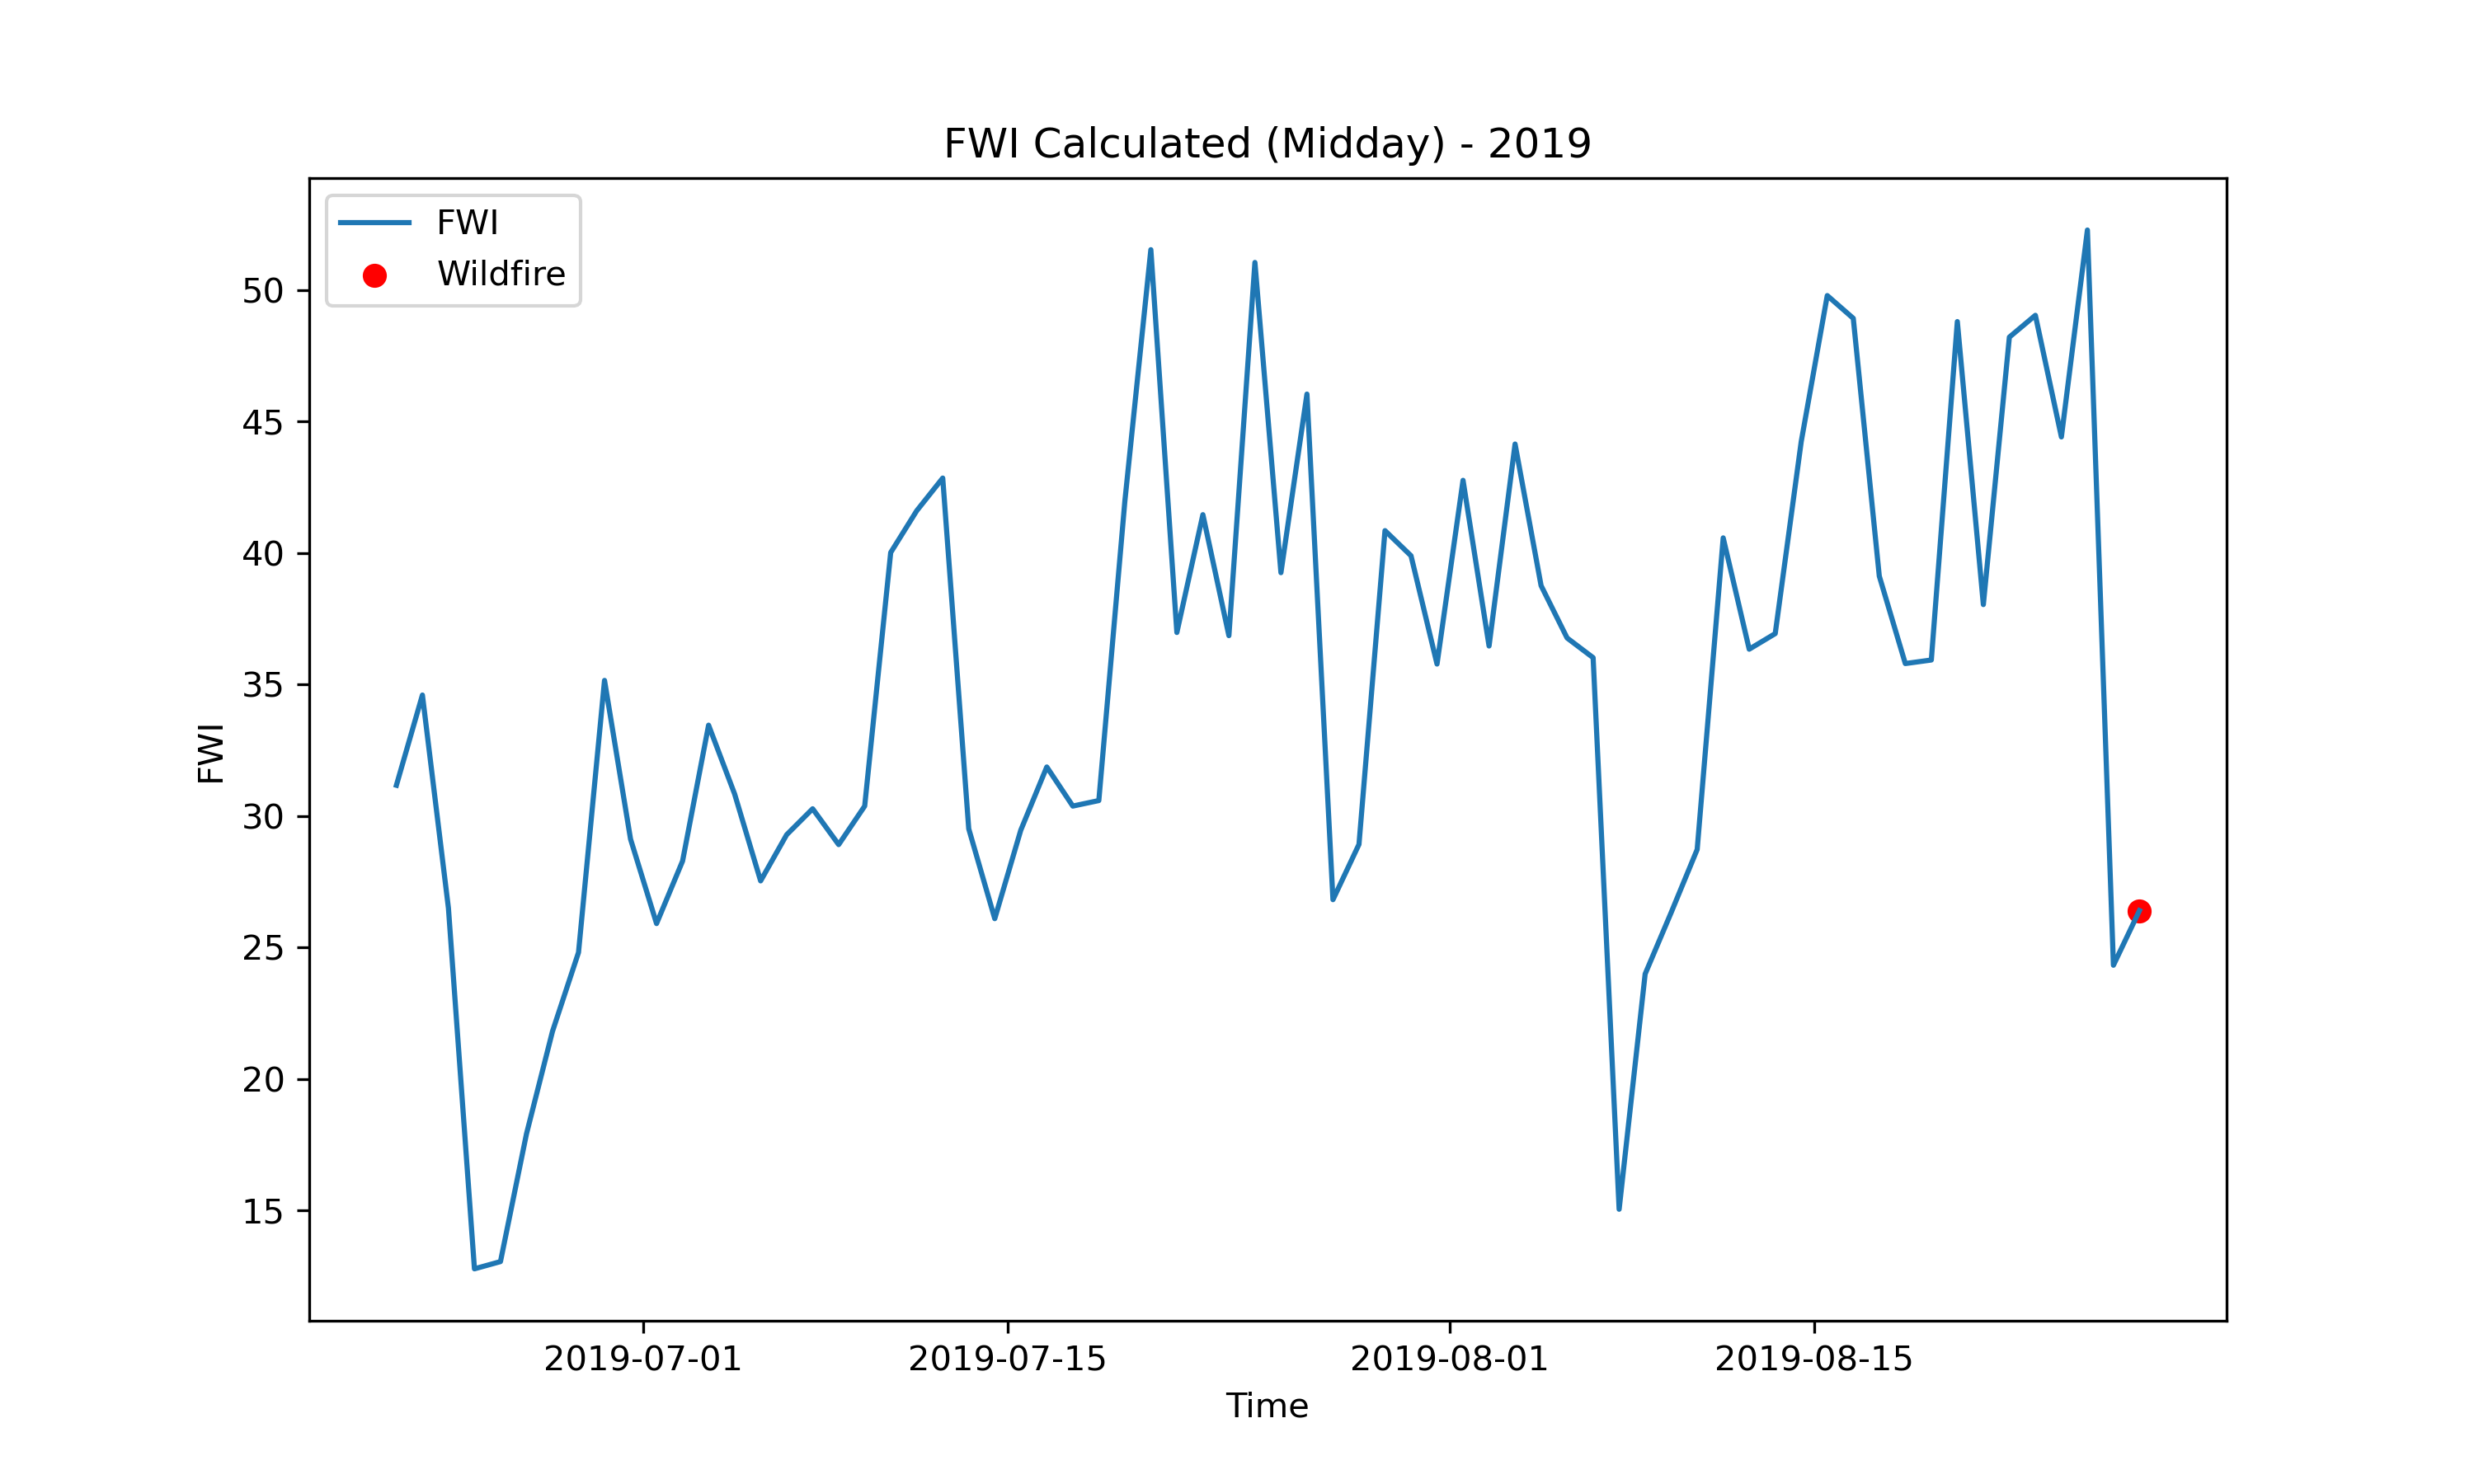
\includegraphics[width=\textwidth]{graphs/2019/2019CalcFWI12.png}
		\caption{FWI - Calculated value}
		\label{fig:fwi_calculated_2019_midday}
	\end{subfigure}
	\label{fig:comparison_fwi_2019_midday_copernicus_calculated}
\end{figure}


\FloatBarrier

\subsection{Fogo de 2022}

\begin{figure}[h]
	\caption{Comparison of FWI calculated values and Copernicus at midday - 2022}
	\centering
	\begin{subfigure}{0.49\textwidth}
		\centering
		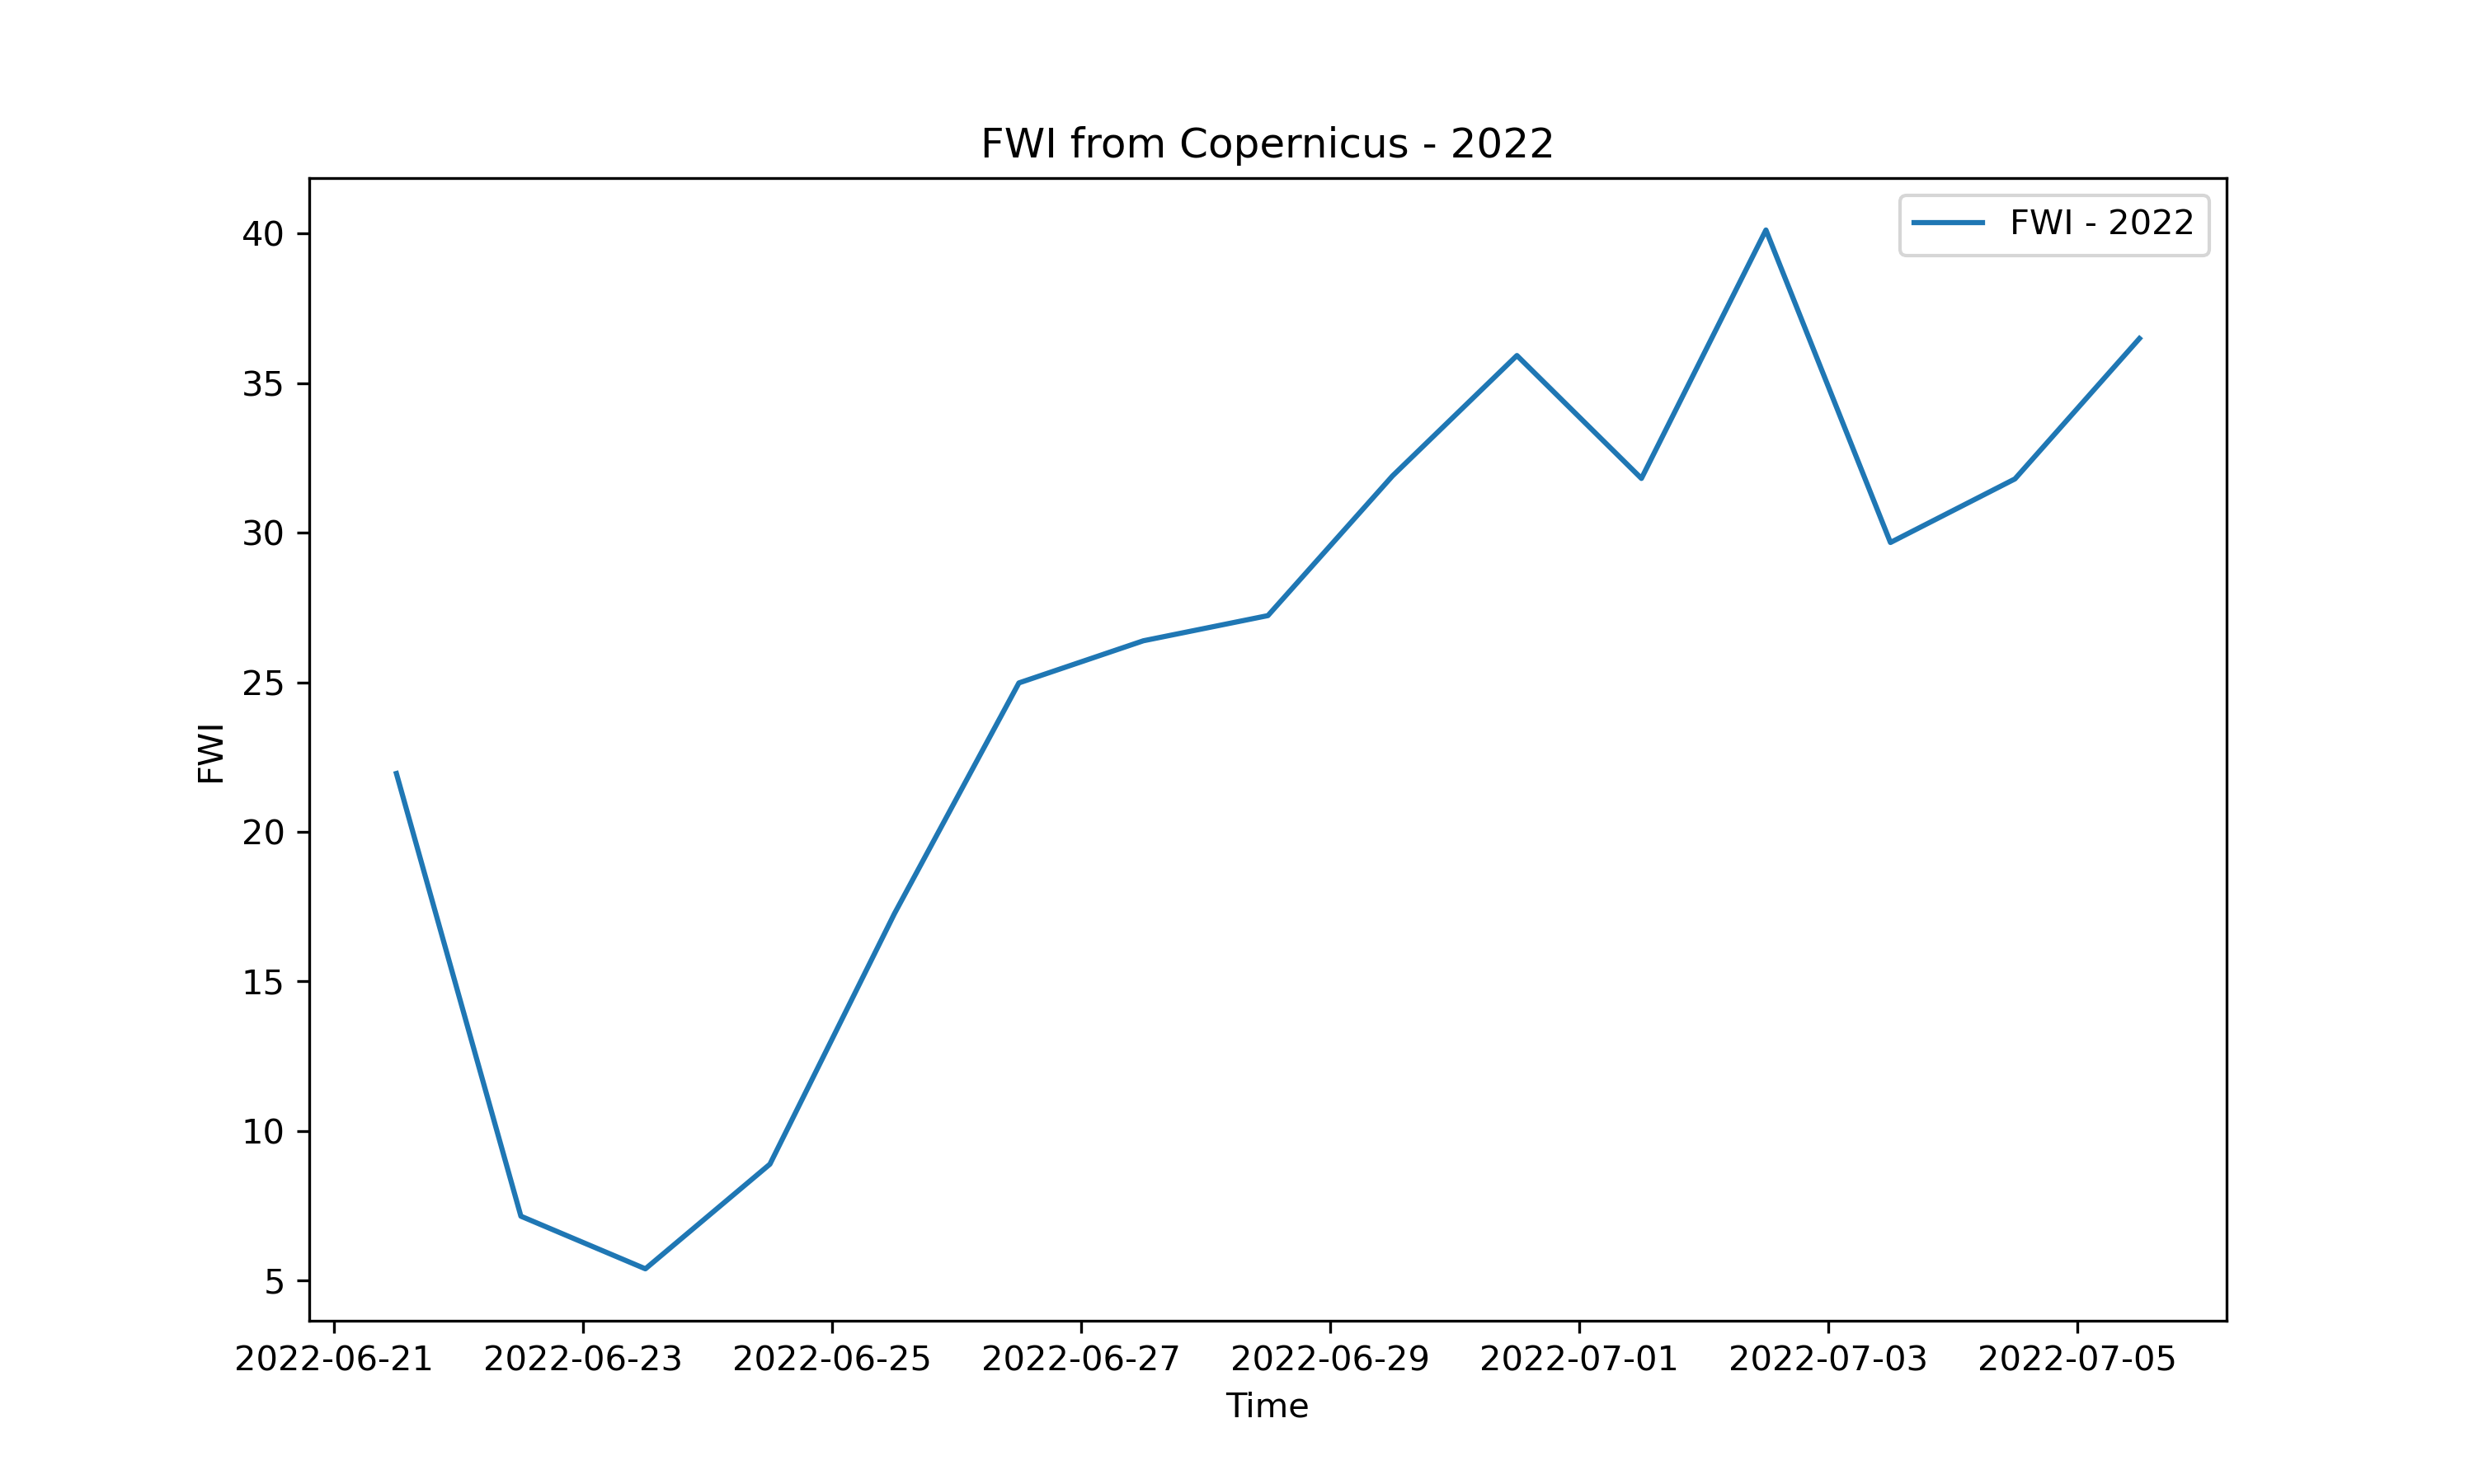
\includegraphics[width=\textwidth]{graphs/2022/2022CopernicusFWI12.png}
		\caption{FWI - Copernicus}
		\label{fig:fwi_copernicus_2022_midday}
	\end{subfigure}
	\hfill
	\begin{subfigure}{0.49\textwidth}
		\centering
		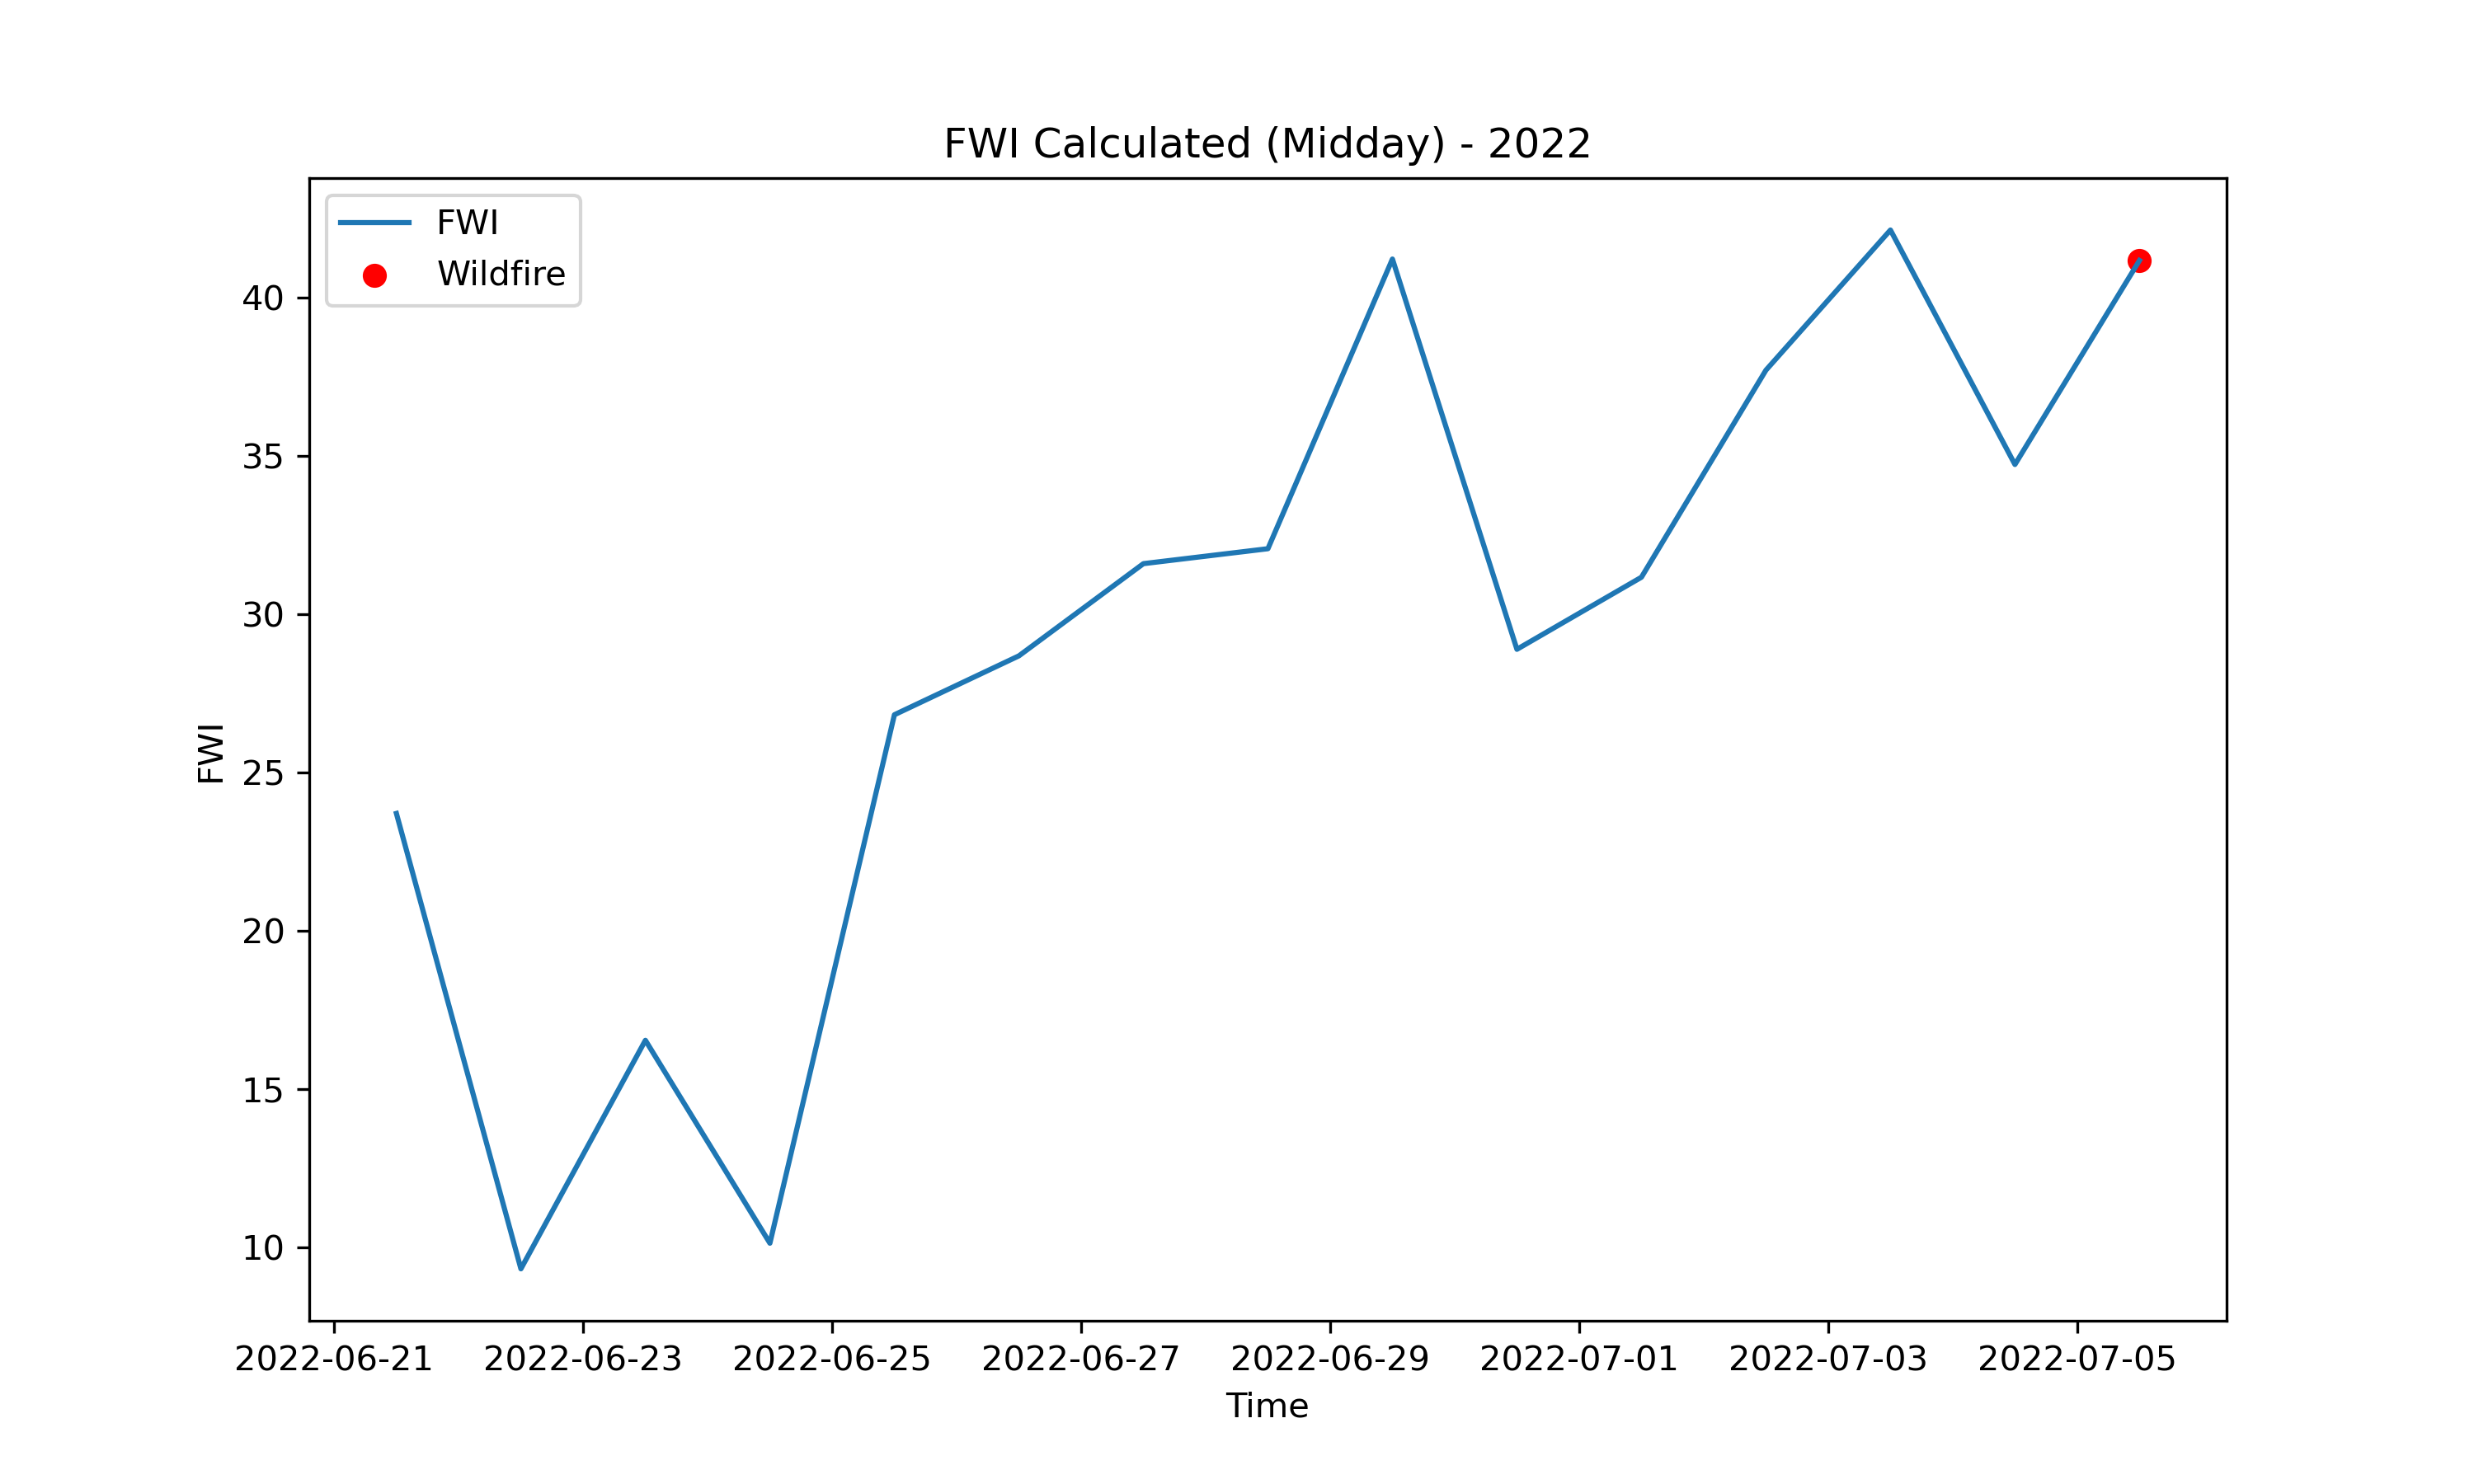
\includegraphics[width=\textwidth]{graphs/2022/2022CalcFWI12Midday.png}
		\caption{FWI - Calculated value}
		\label{fig:fwi_calculated_2022_midday}
	\end{subfigure}
	\label{fig:comparison_fwi_2022_midday_copernicus_calculated}
\end{figure}

\FloatBarrier

\section{Hourly FWI variables}
\begin{figure}[h]
	\centering
	\caption{Calculated hourly FWI value for 2015, 2019, and 2022}
	\begin{subfigure}{0.45\textwidth}
		\centering
		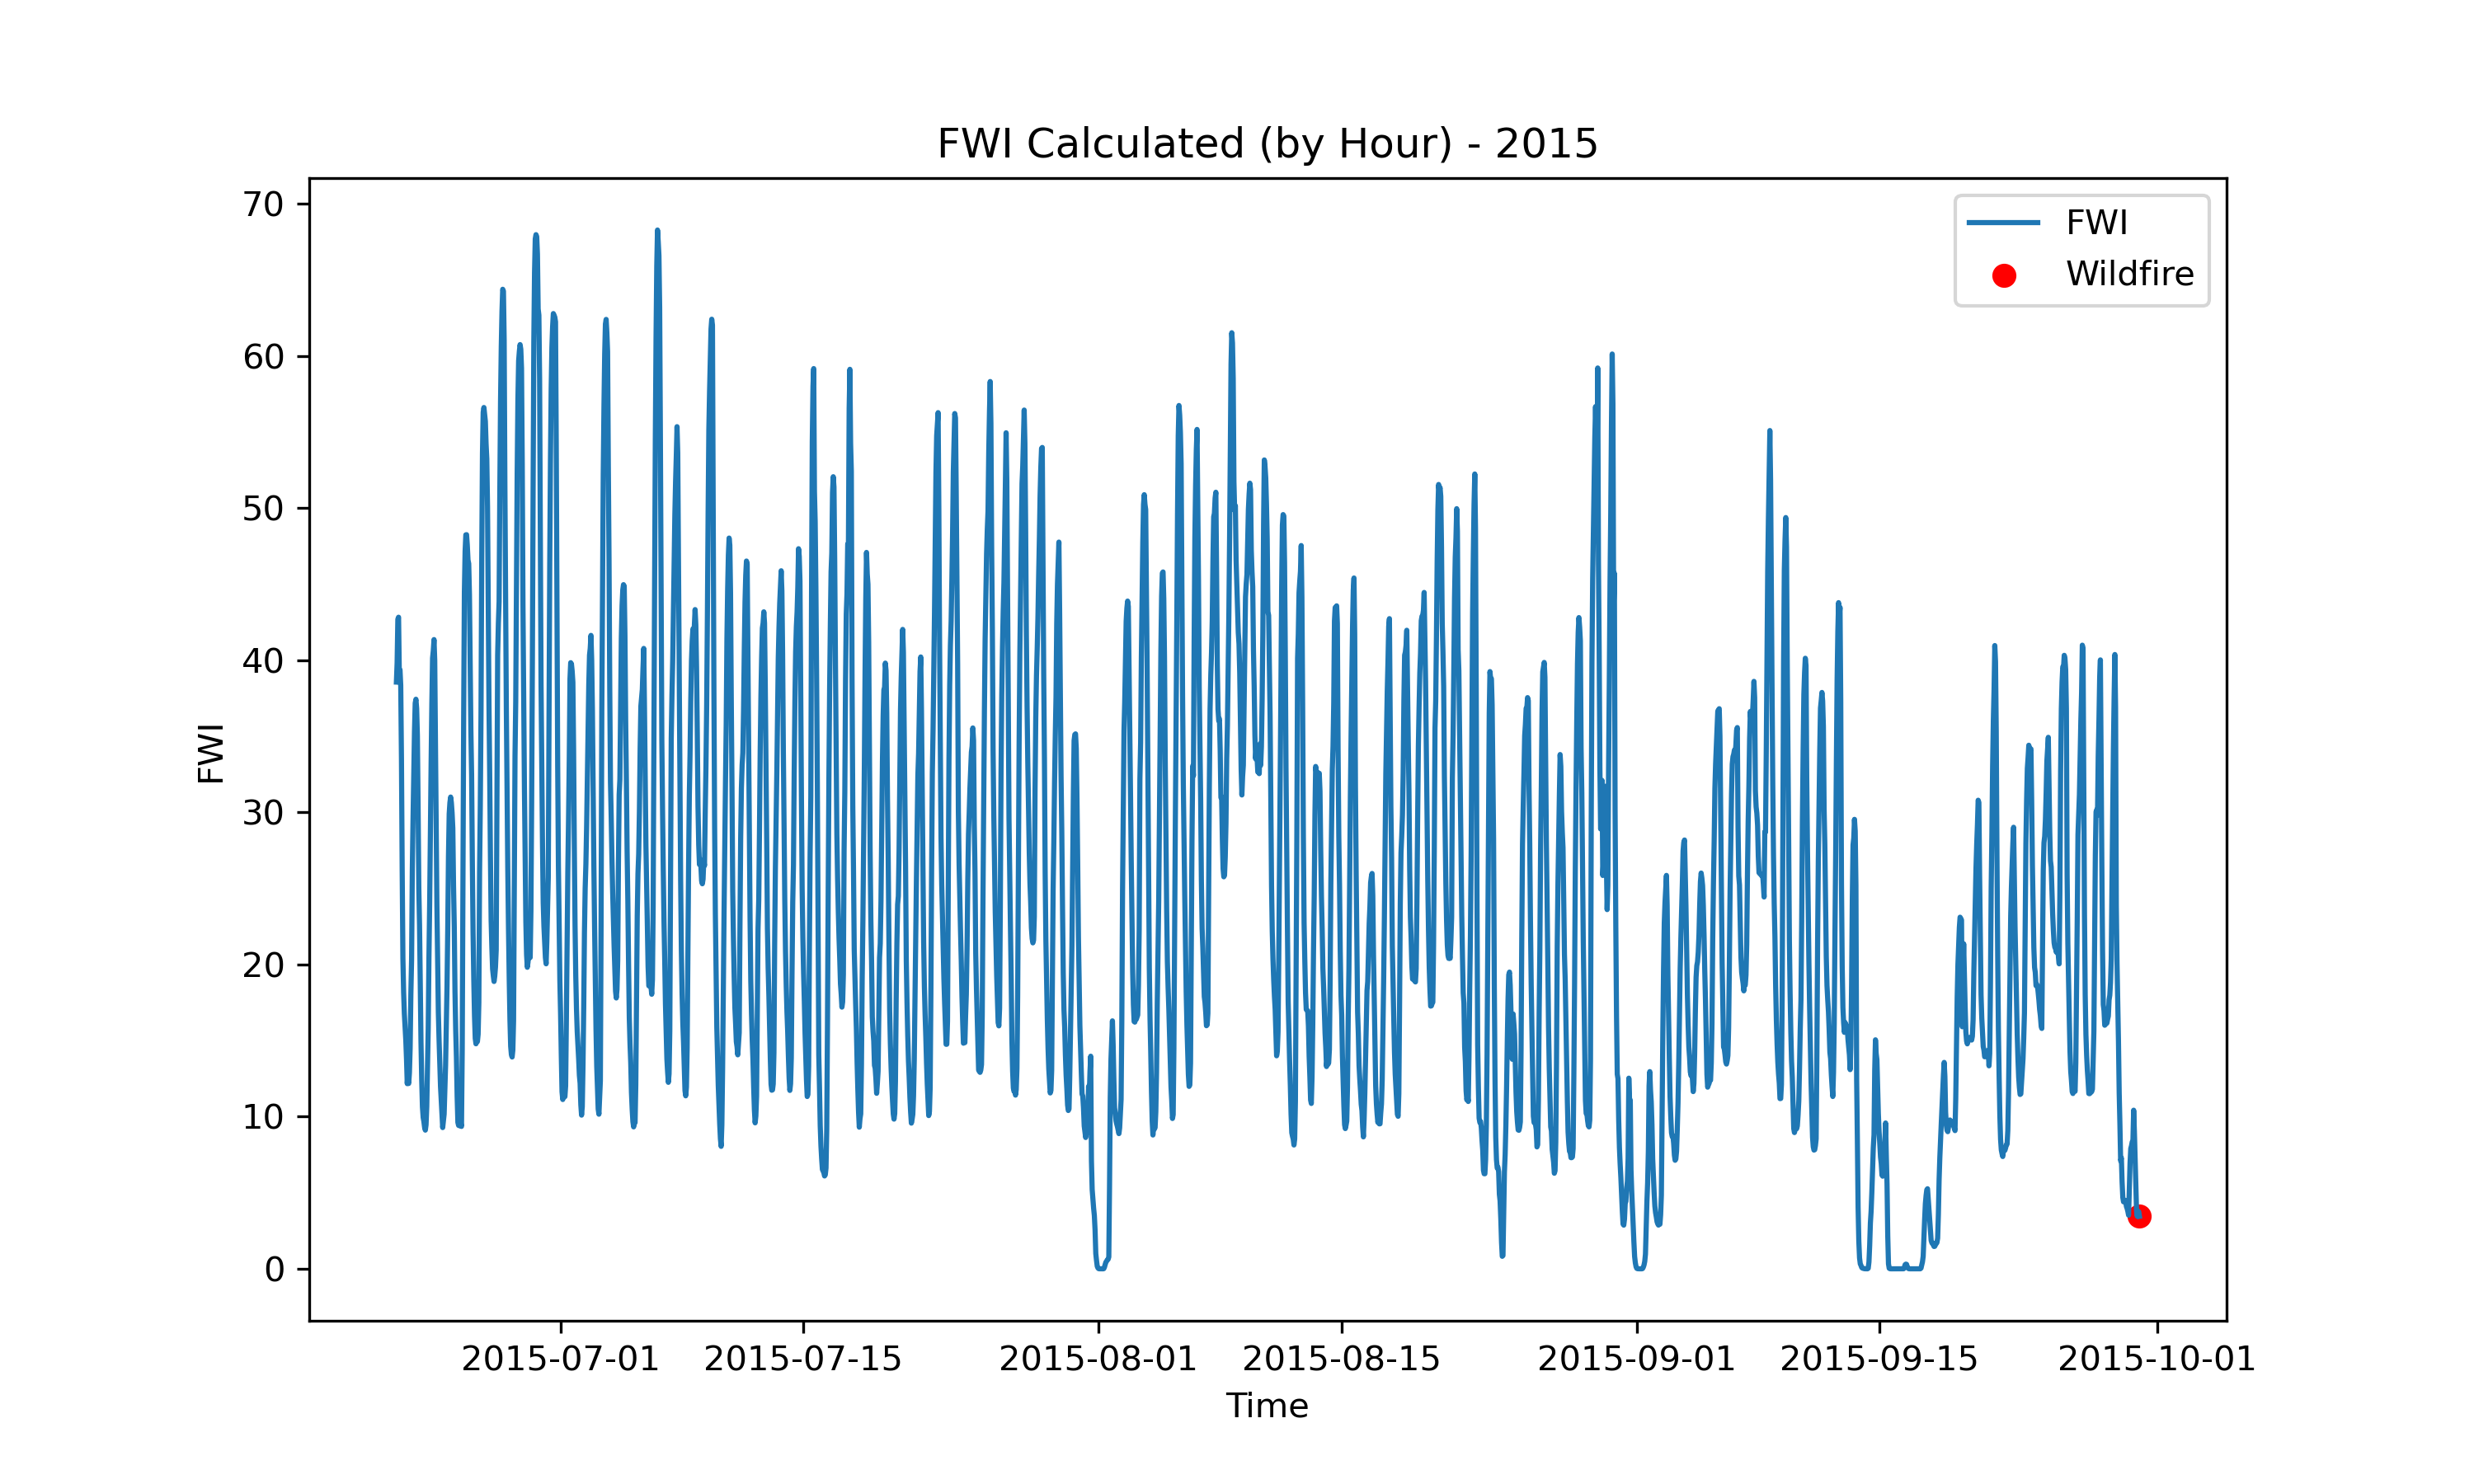
\includegraphics[width=\textwidth]{graphs/2015/byHour/2015CalcFWI12.png}
	\end{subfigure}
	\hfill
	\begin{subfigure}{0.45\textwidth}
		\centering
		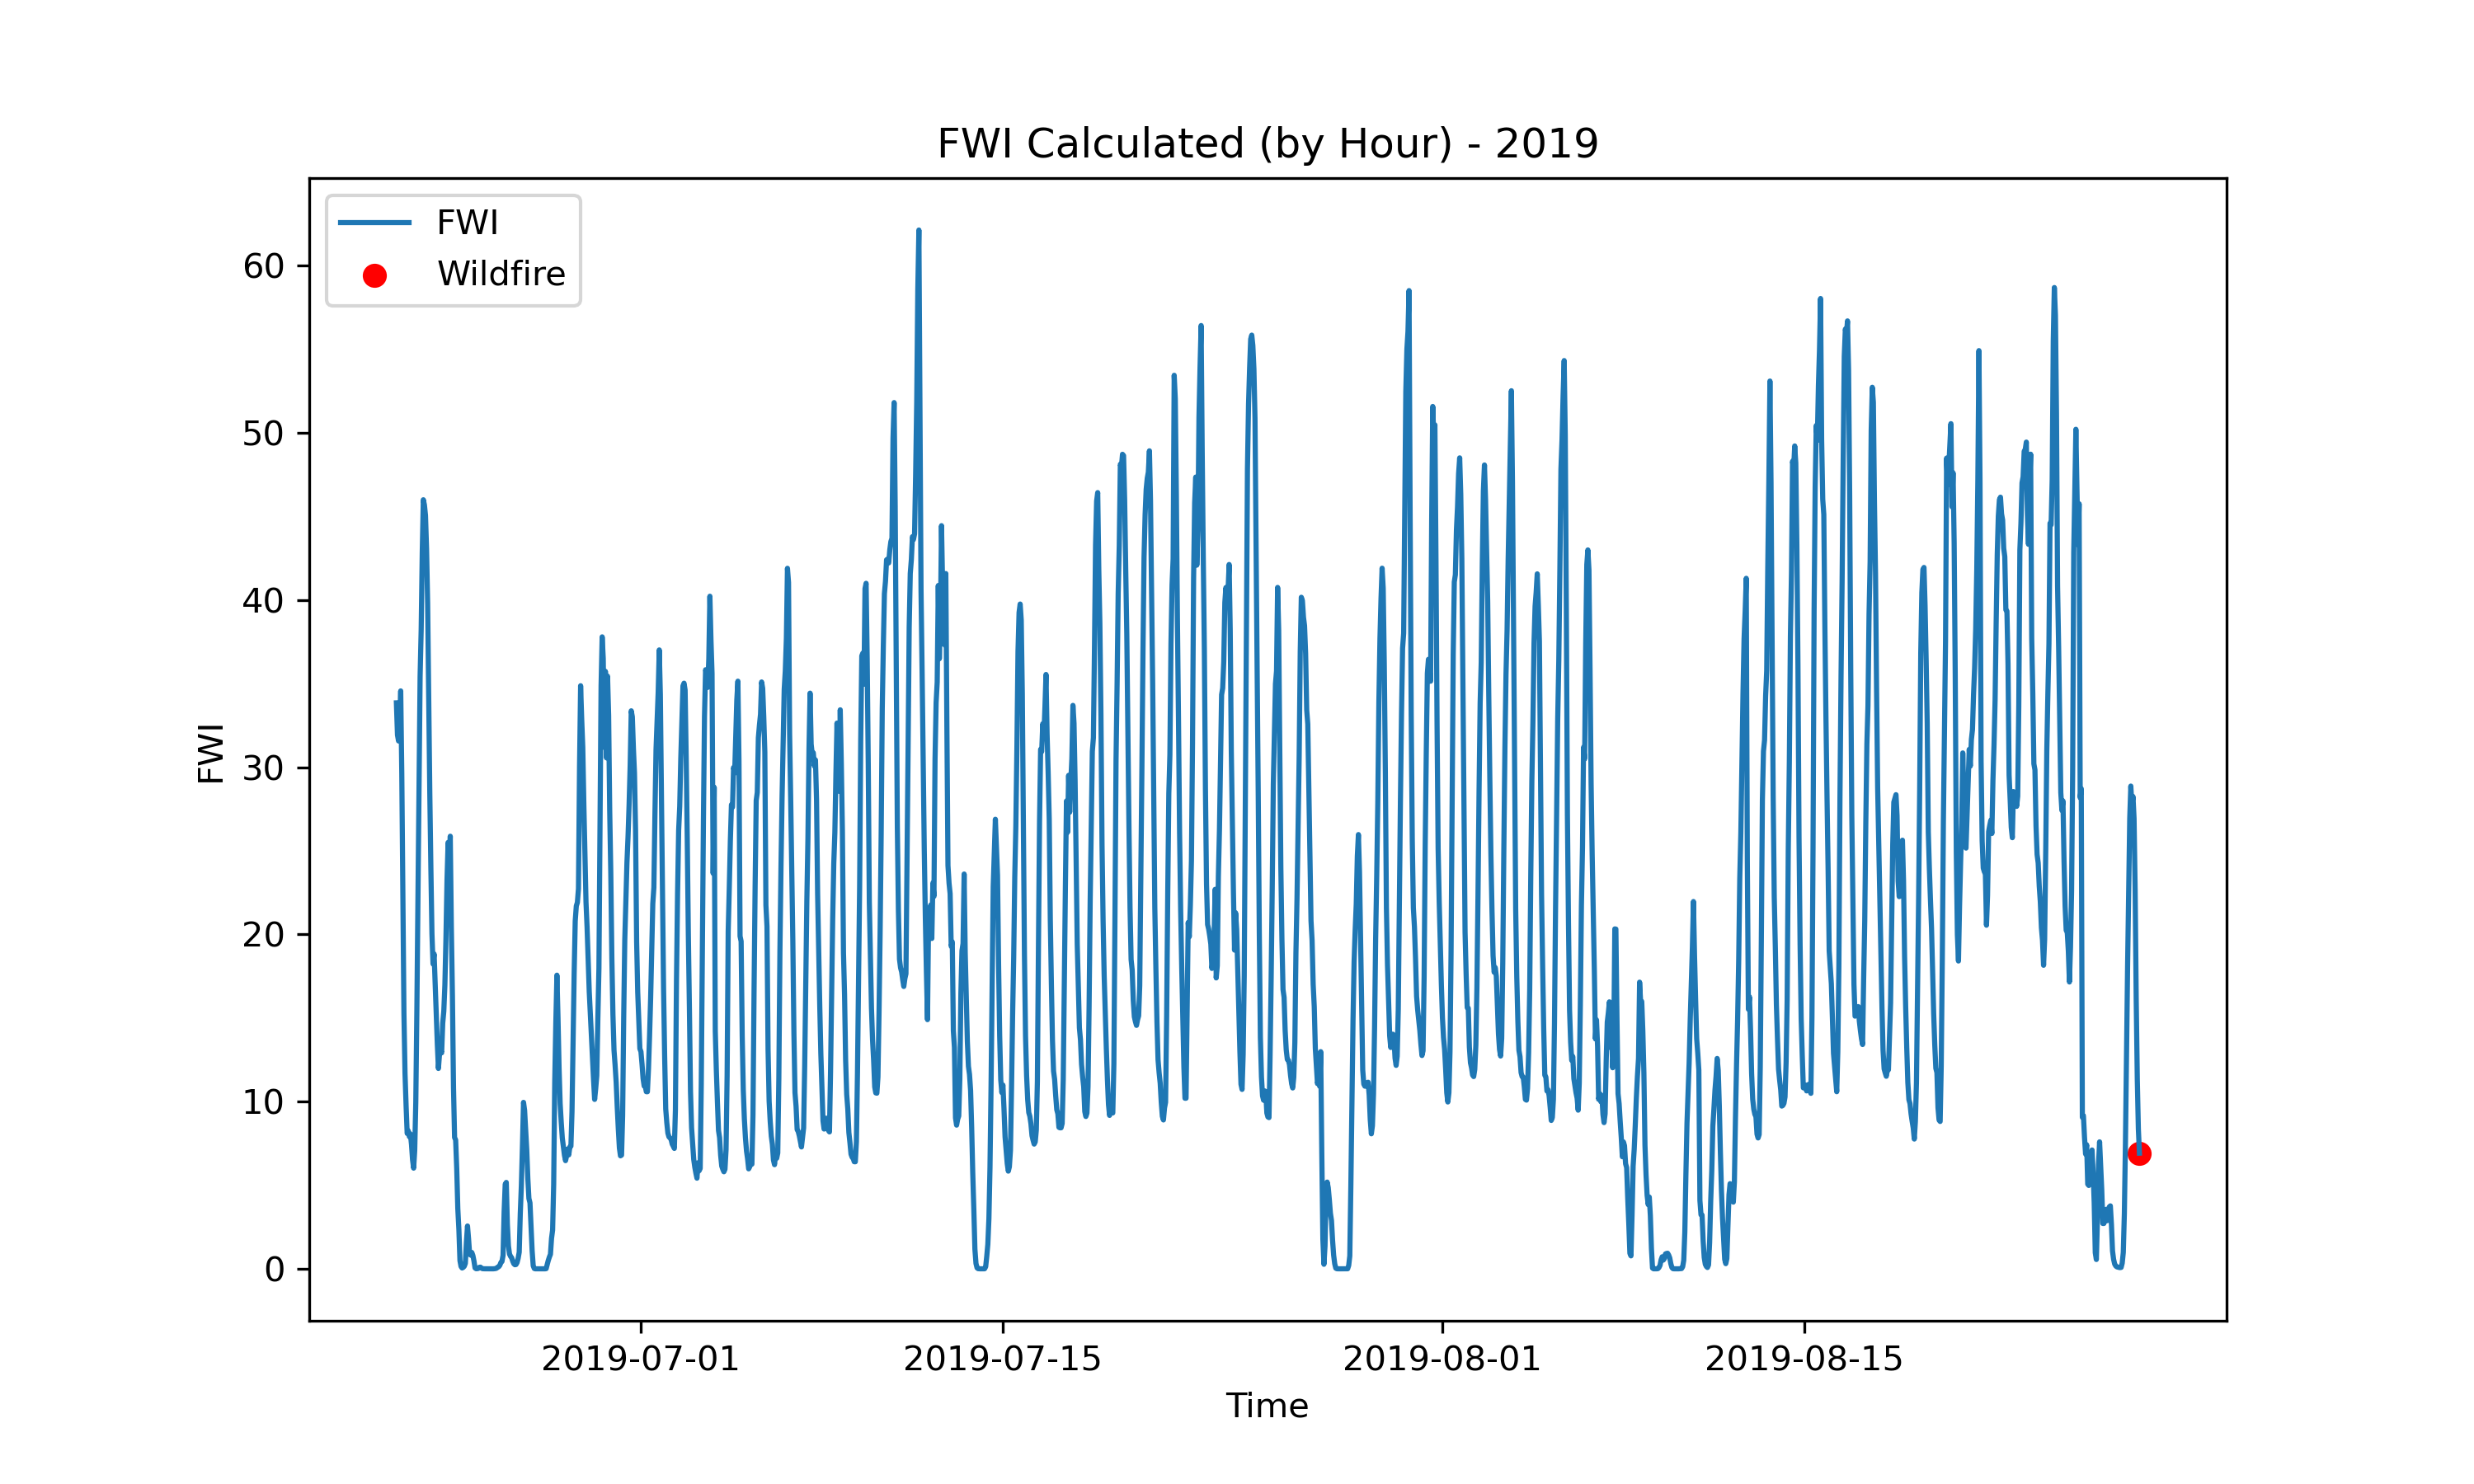
\includegraphics[width=\textwidth]{graphs/2019/byHour/2019CalcFWI12.png}
	\end{subfigure}
	
	\begin{subfigure}{0.45\textwidth}
		\centering
		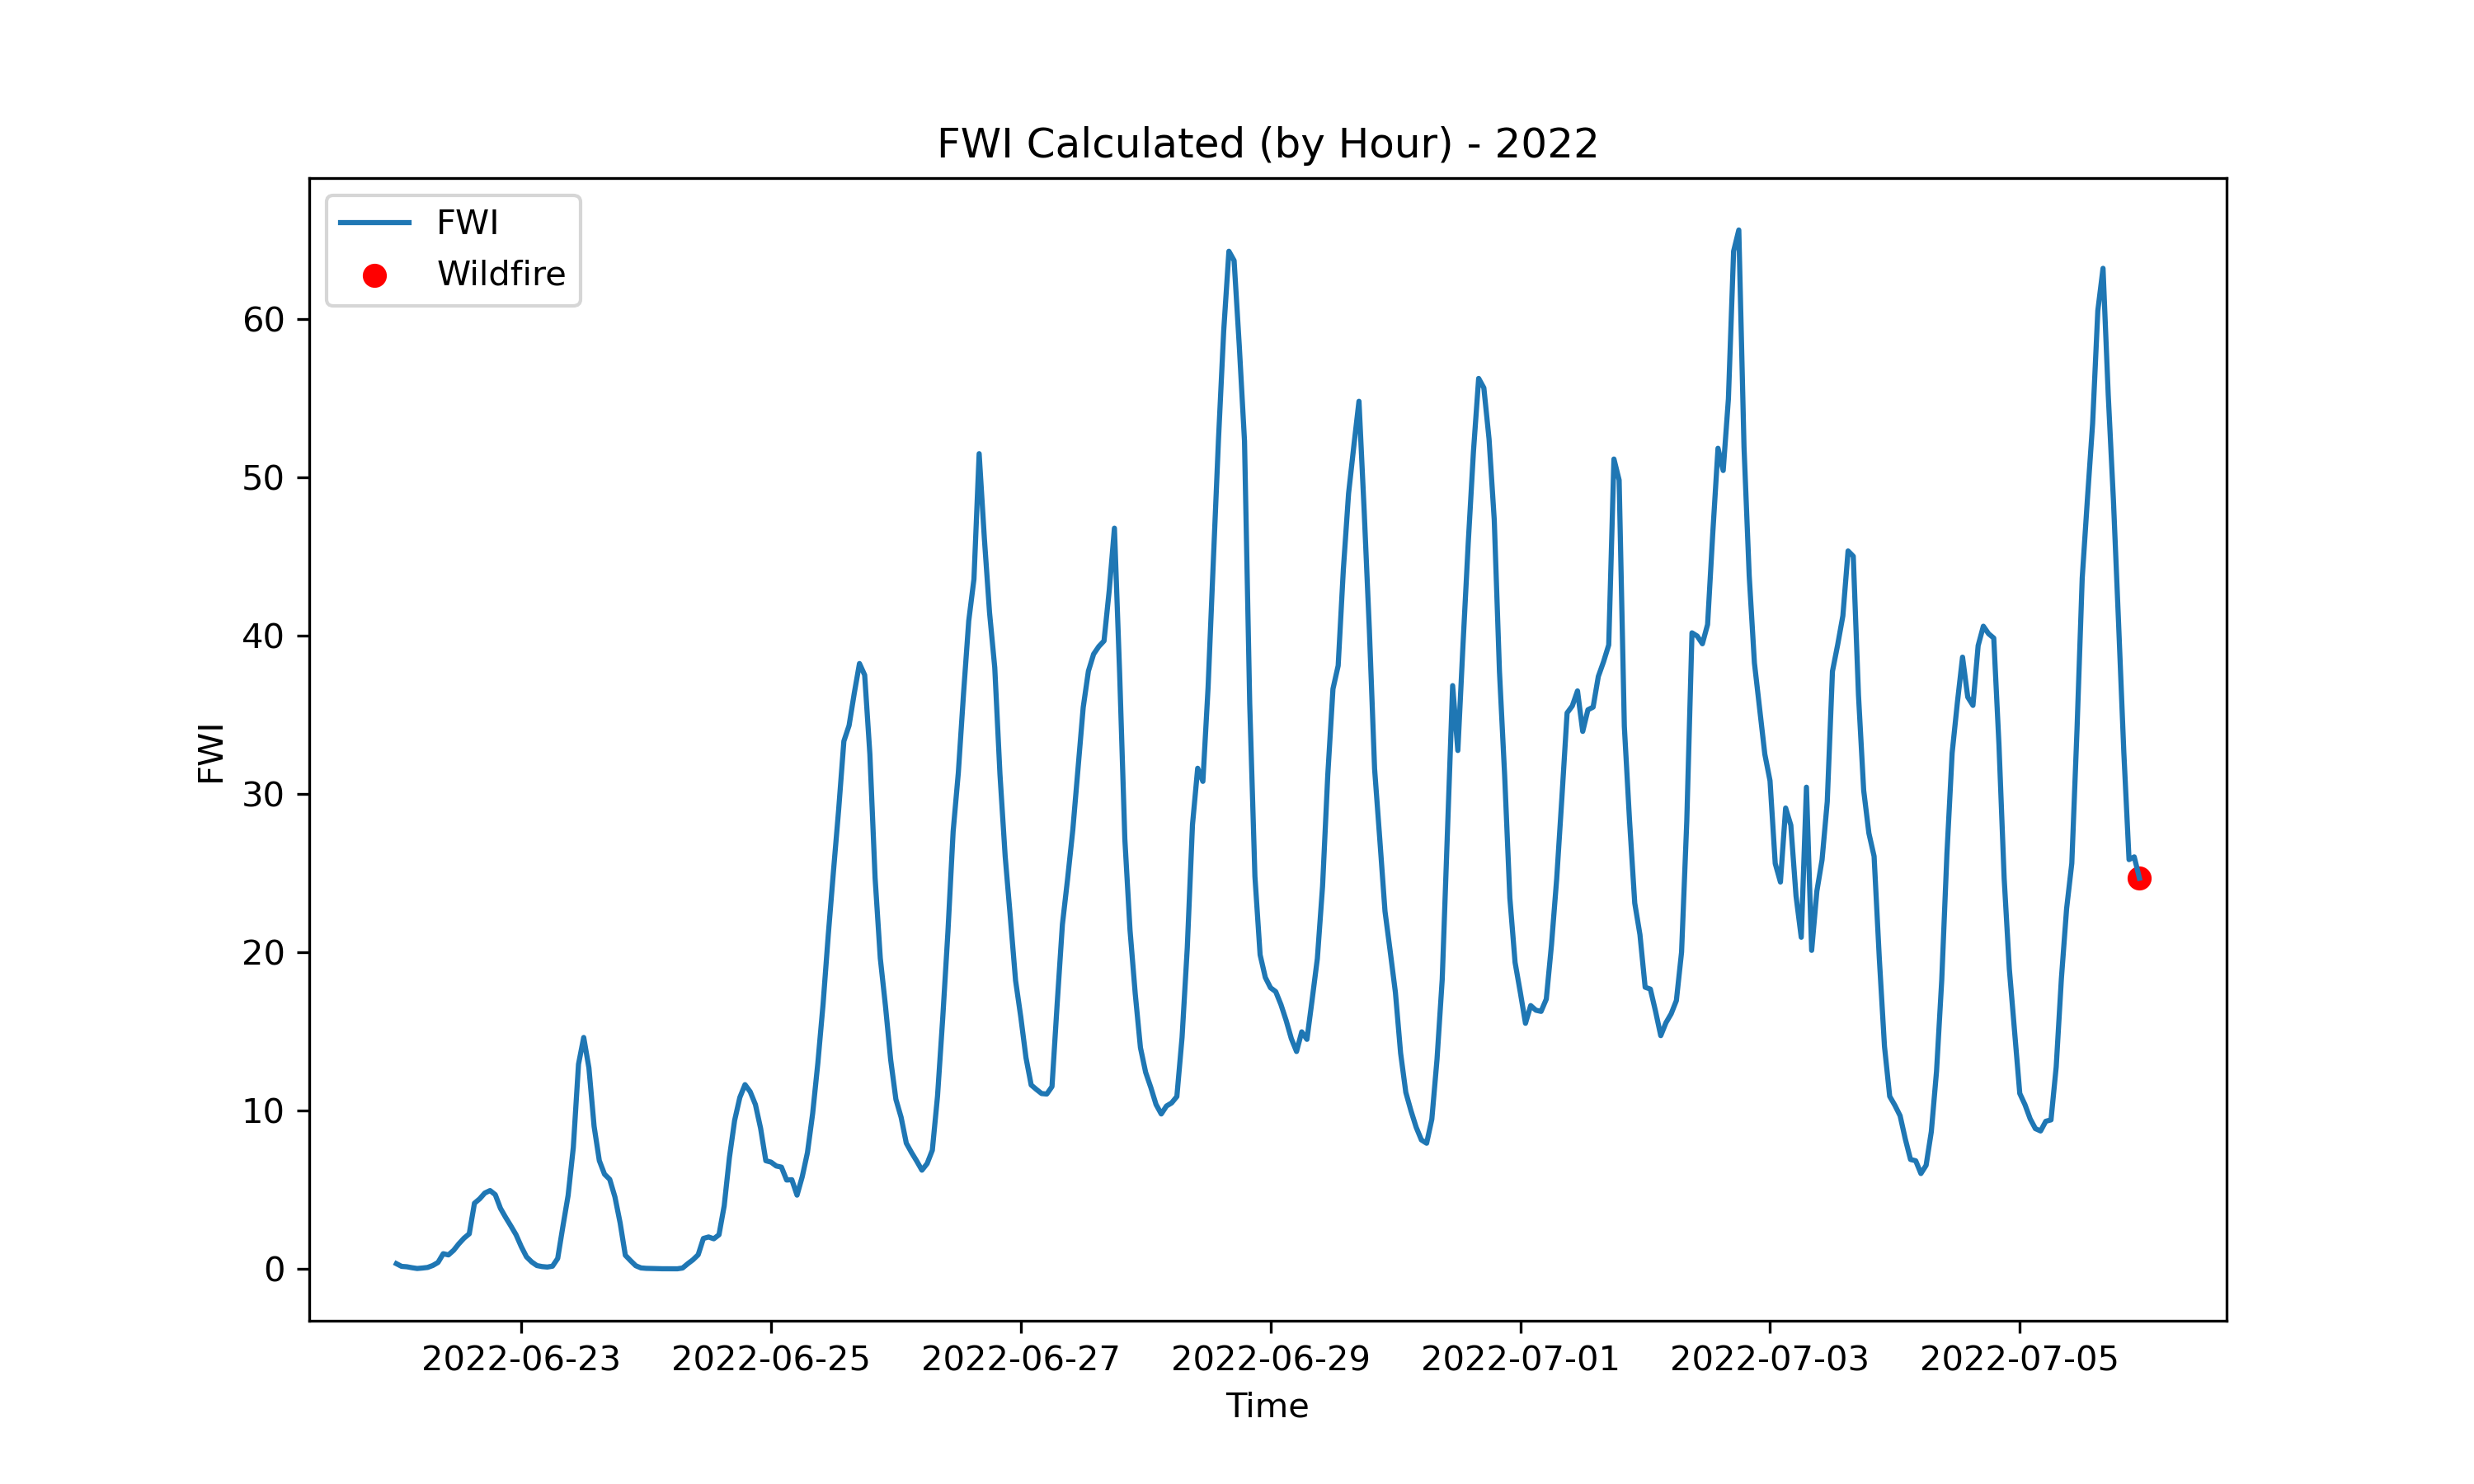
\includegraphics[width=\textwidth]{graphs/2022/2022CalcFWI12.png}
	\end{subfigure}
	
	\label{fig:hourly_fwi}
\end{figure}

\begin{figure}[h]
	\centering
	\caption{Calculated hourly FFMC value for 2015, 2019, and 2022}
	\begin{subfigure}{0.45\textwidth}
		\centering
		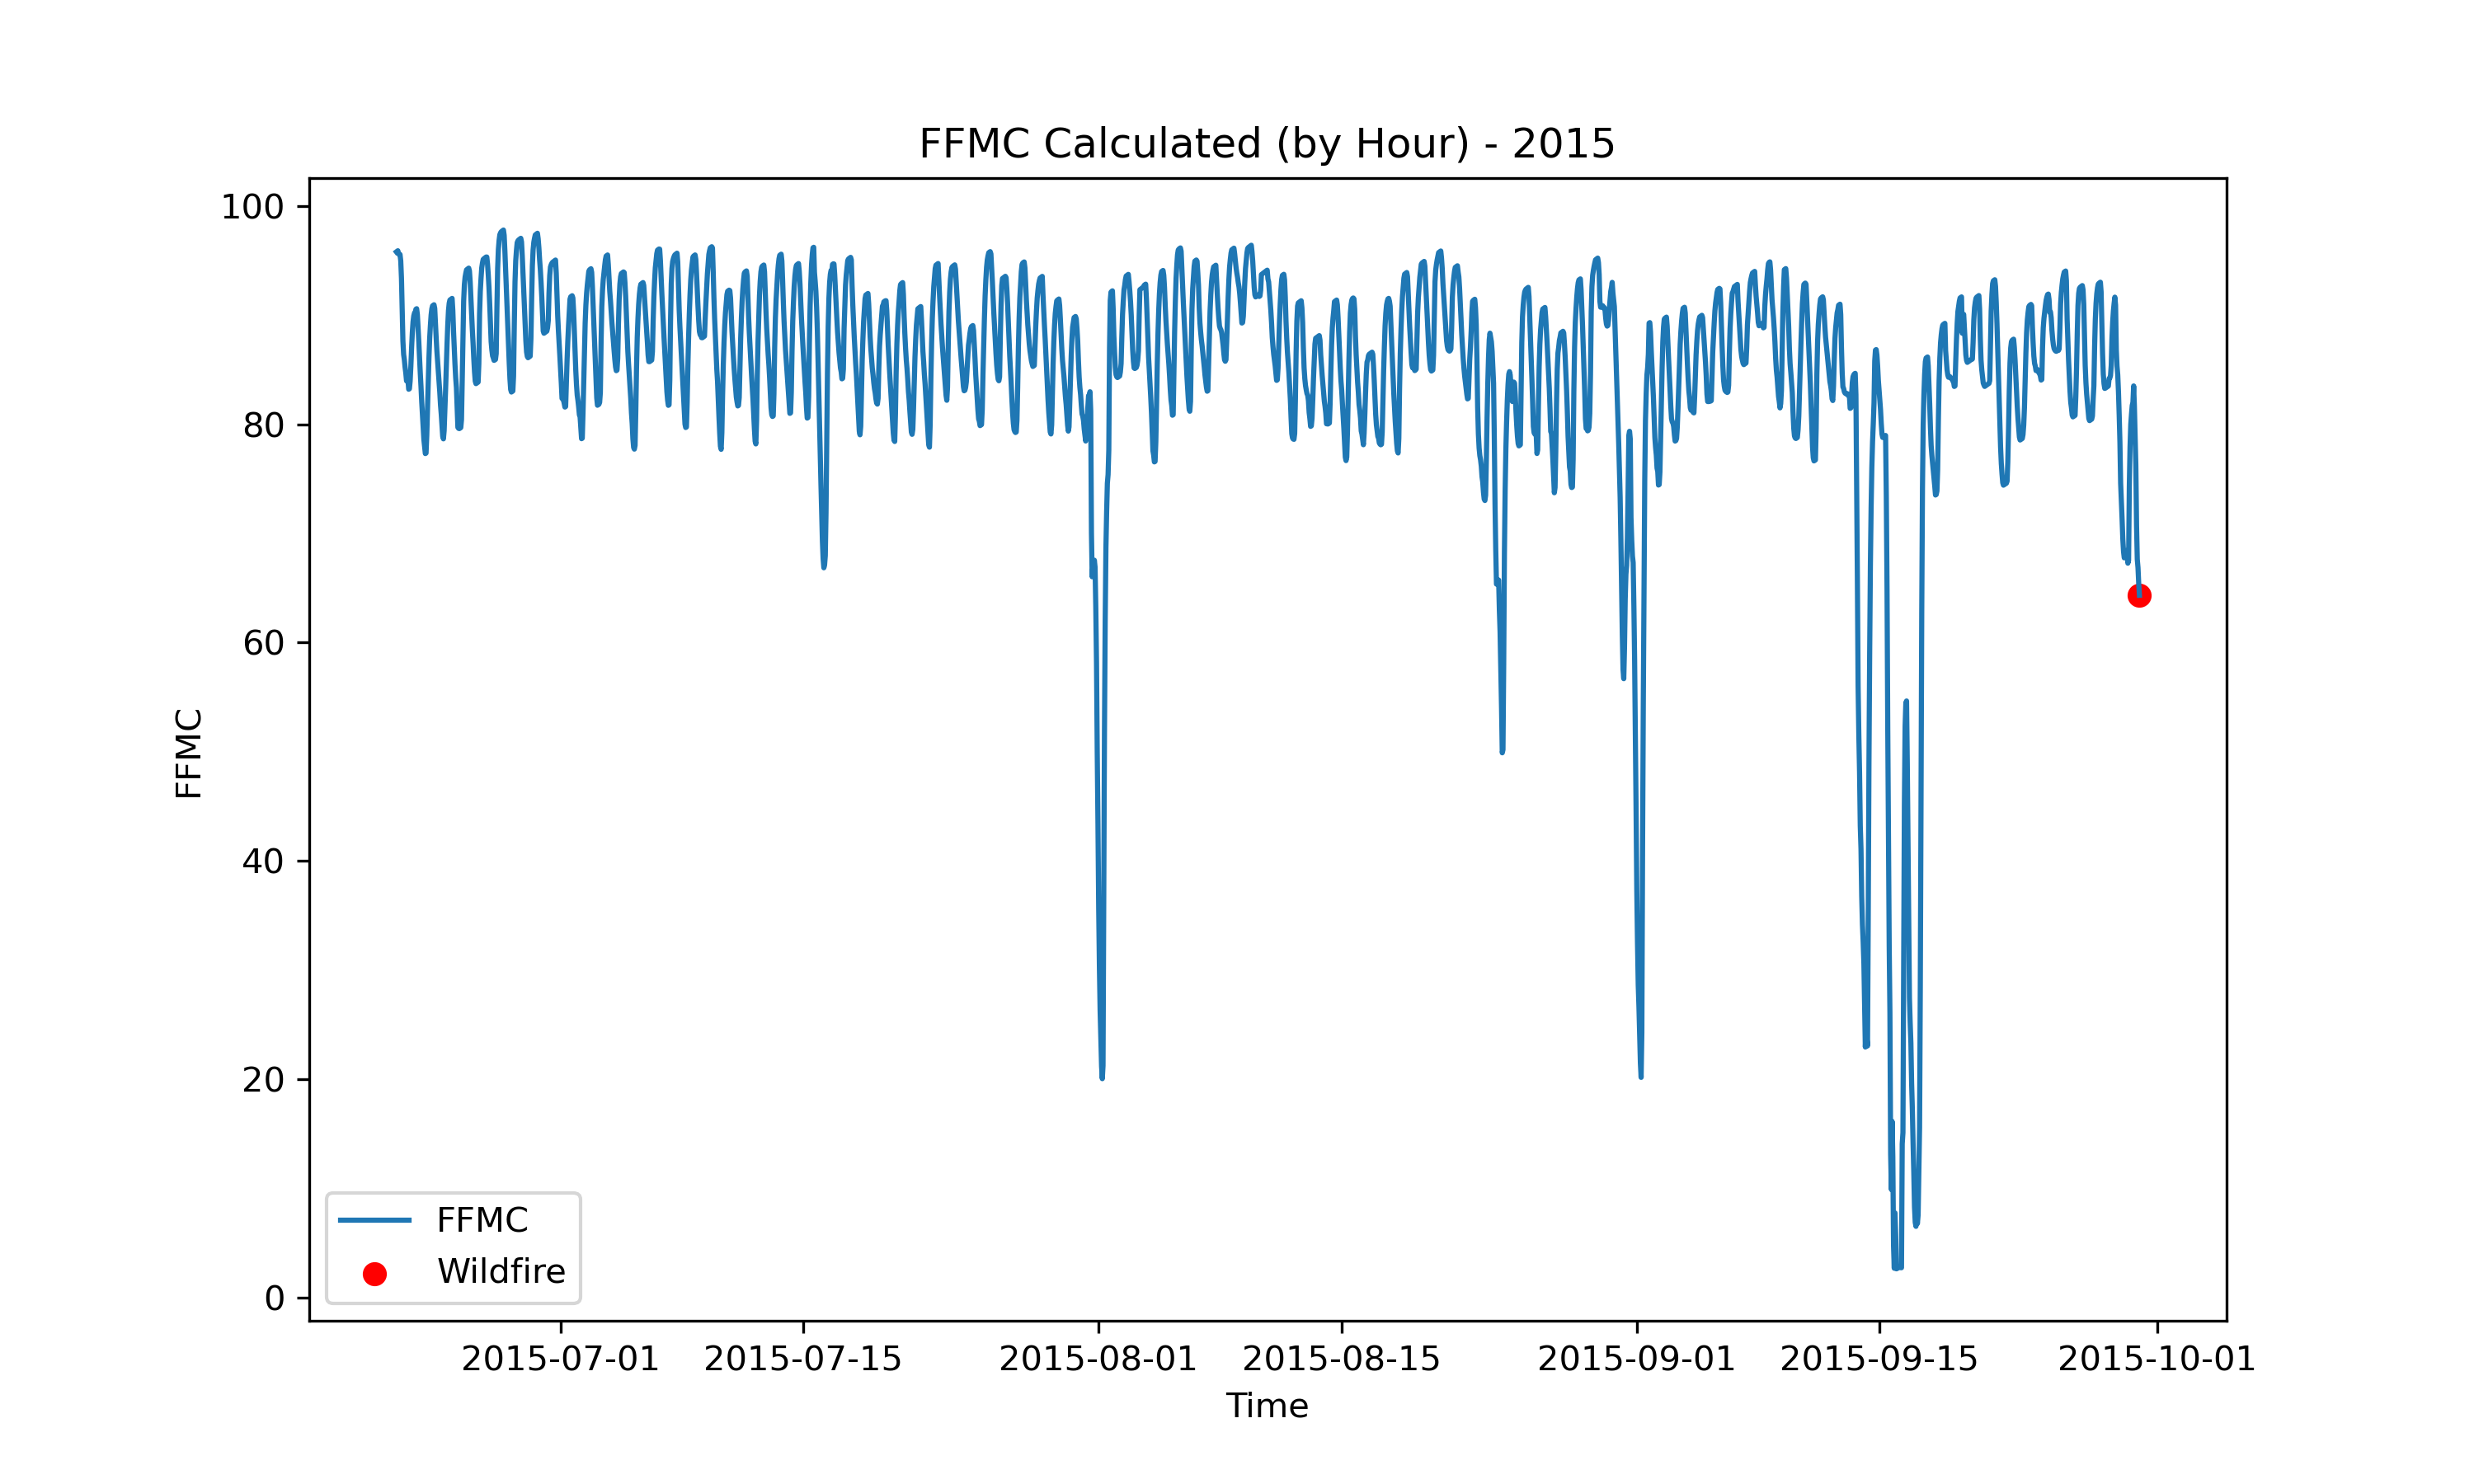
\includegraphics[width=\textwidth]{graphs/2015/byHour/2015CalcFFMC12.png}
	\end{subfigure}
	\hfill
	\begin{subfigure}{0.45\textwidth}
		\centering
		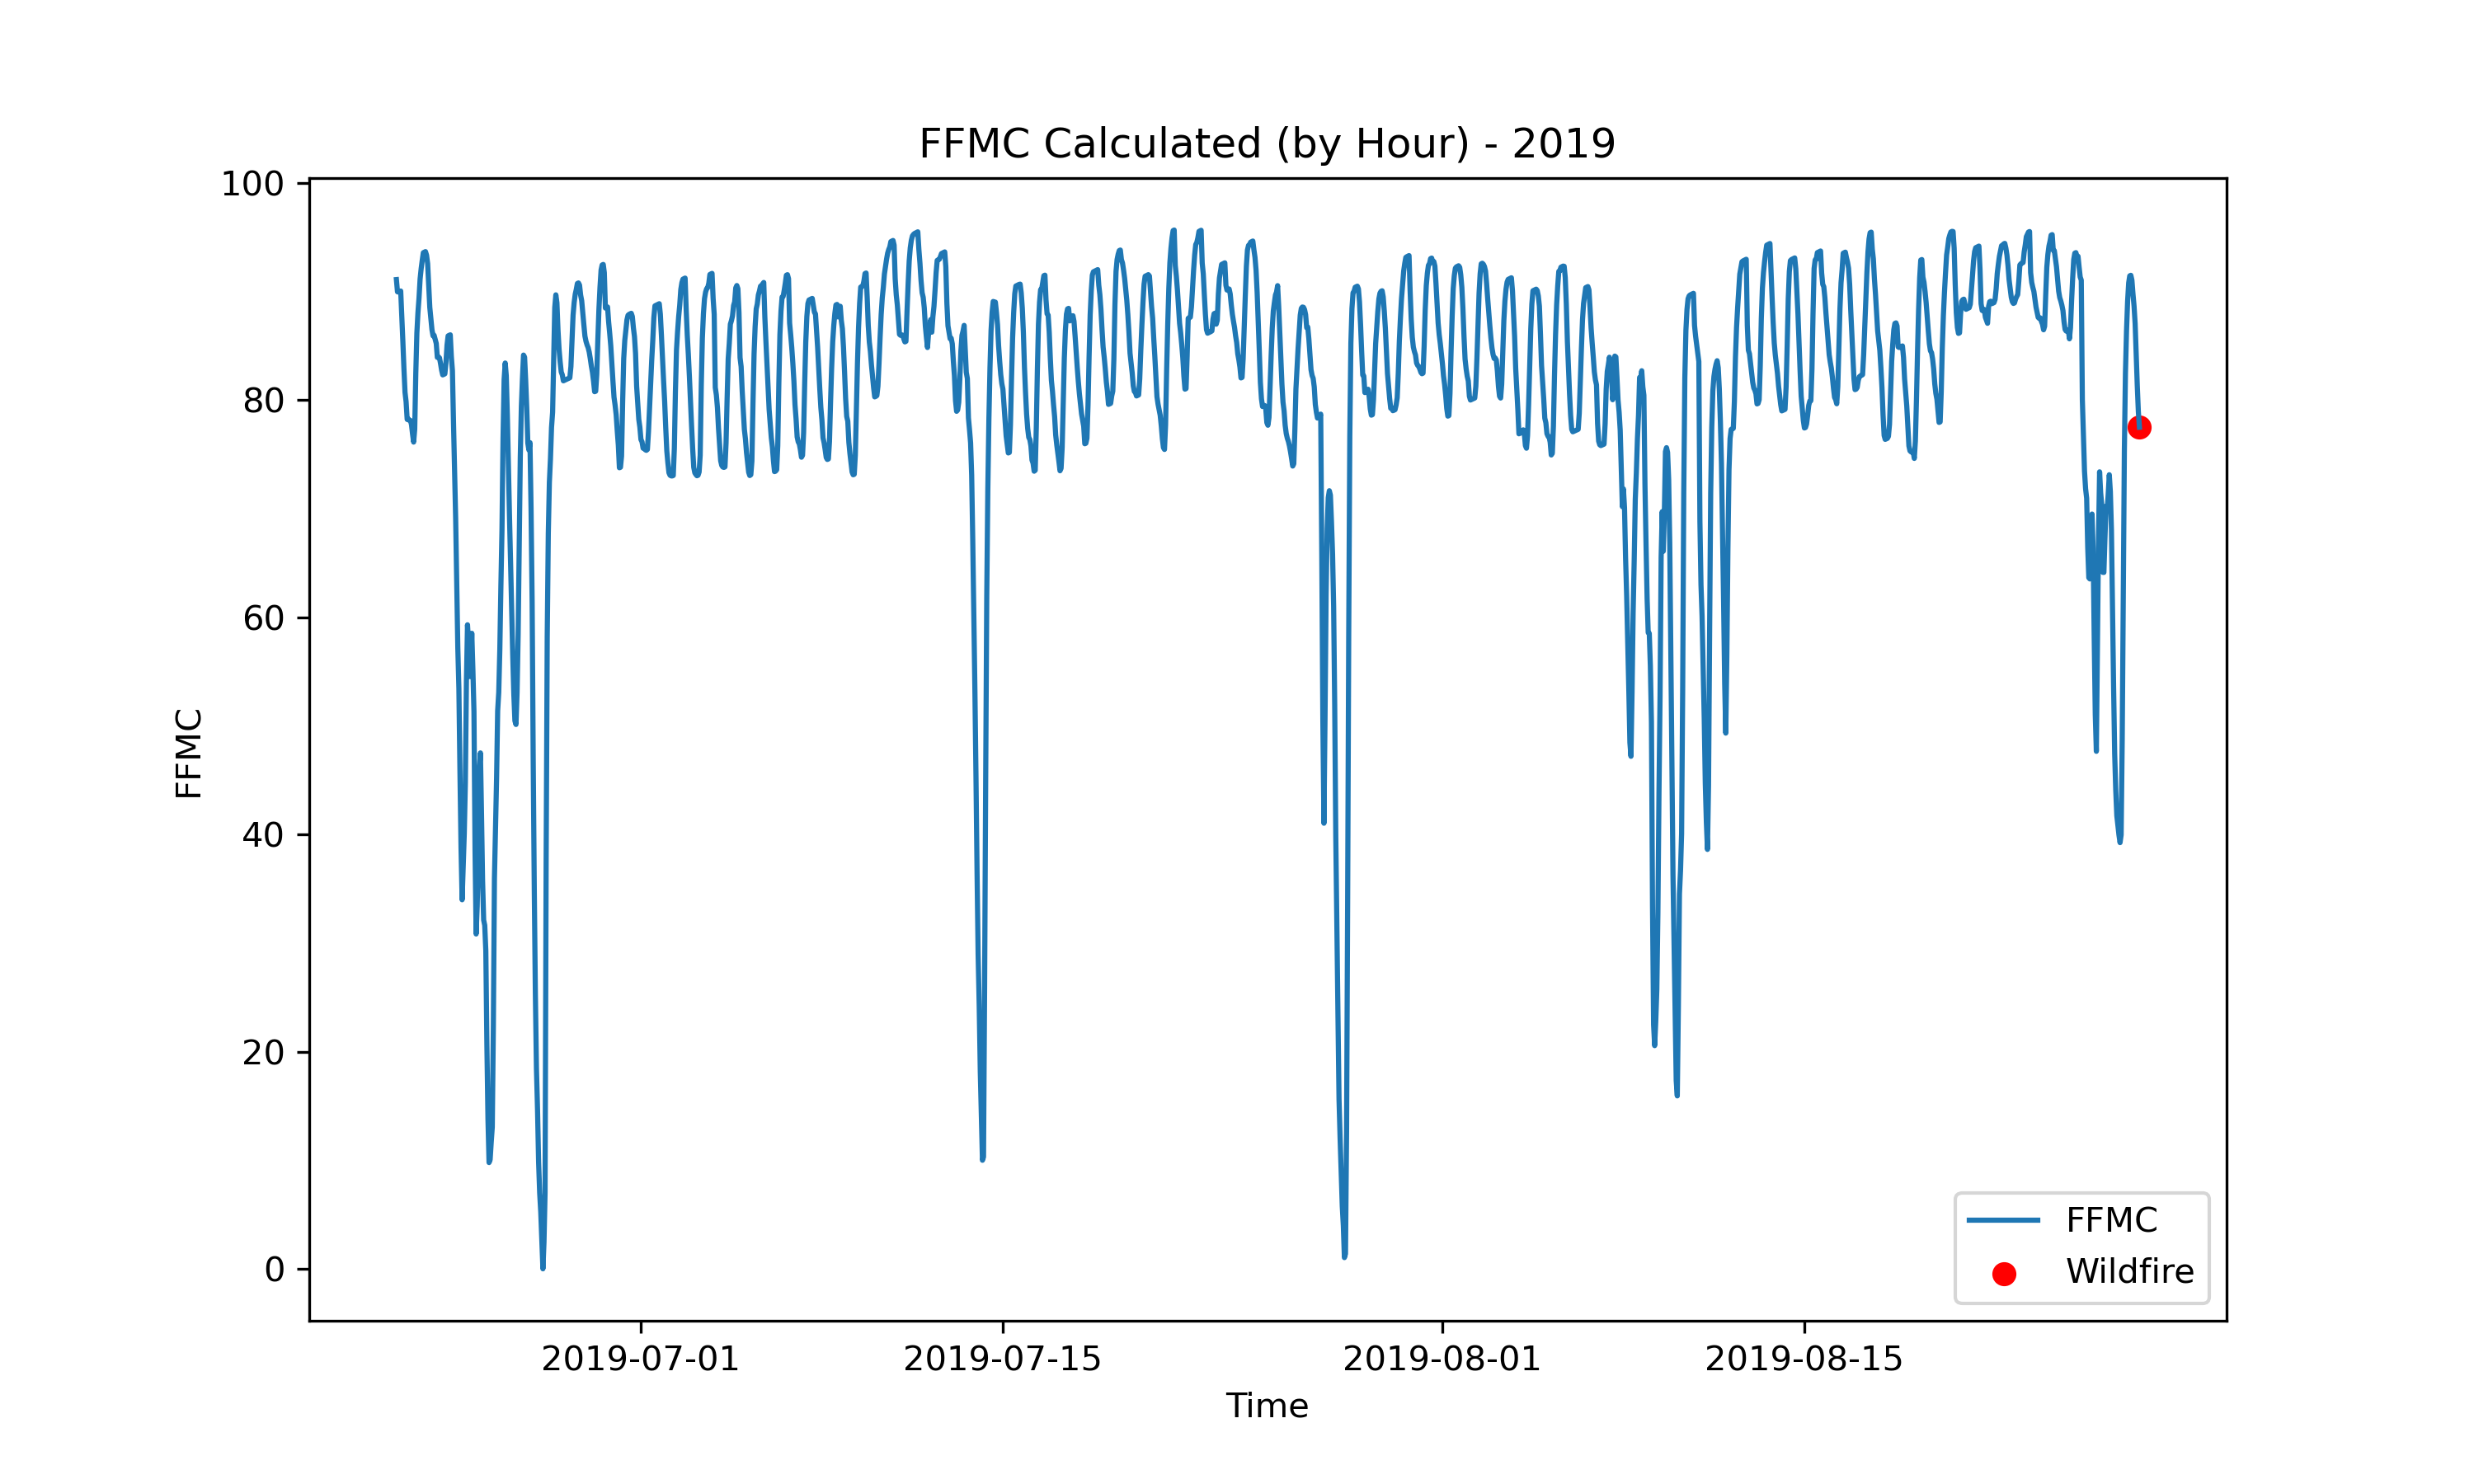
\includegraphics[width=\textwidth]{graphs/2019/2019CalcFFMC12.png}
	\end{subfigure}
	\hfill
	\begin{subfigure}{0.45\textwidth}
		\centering
		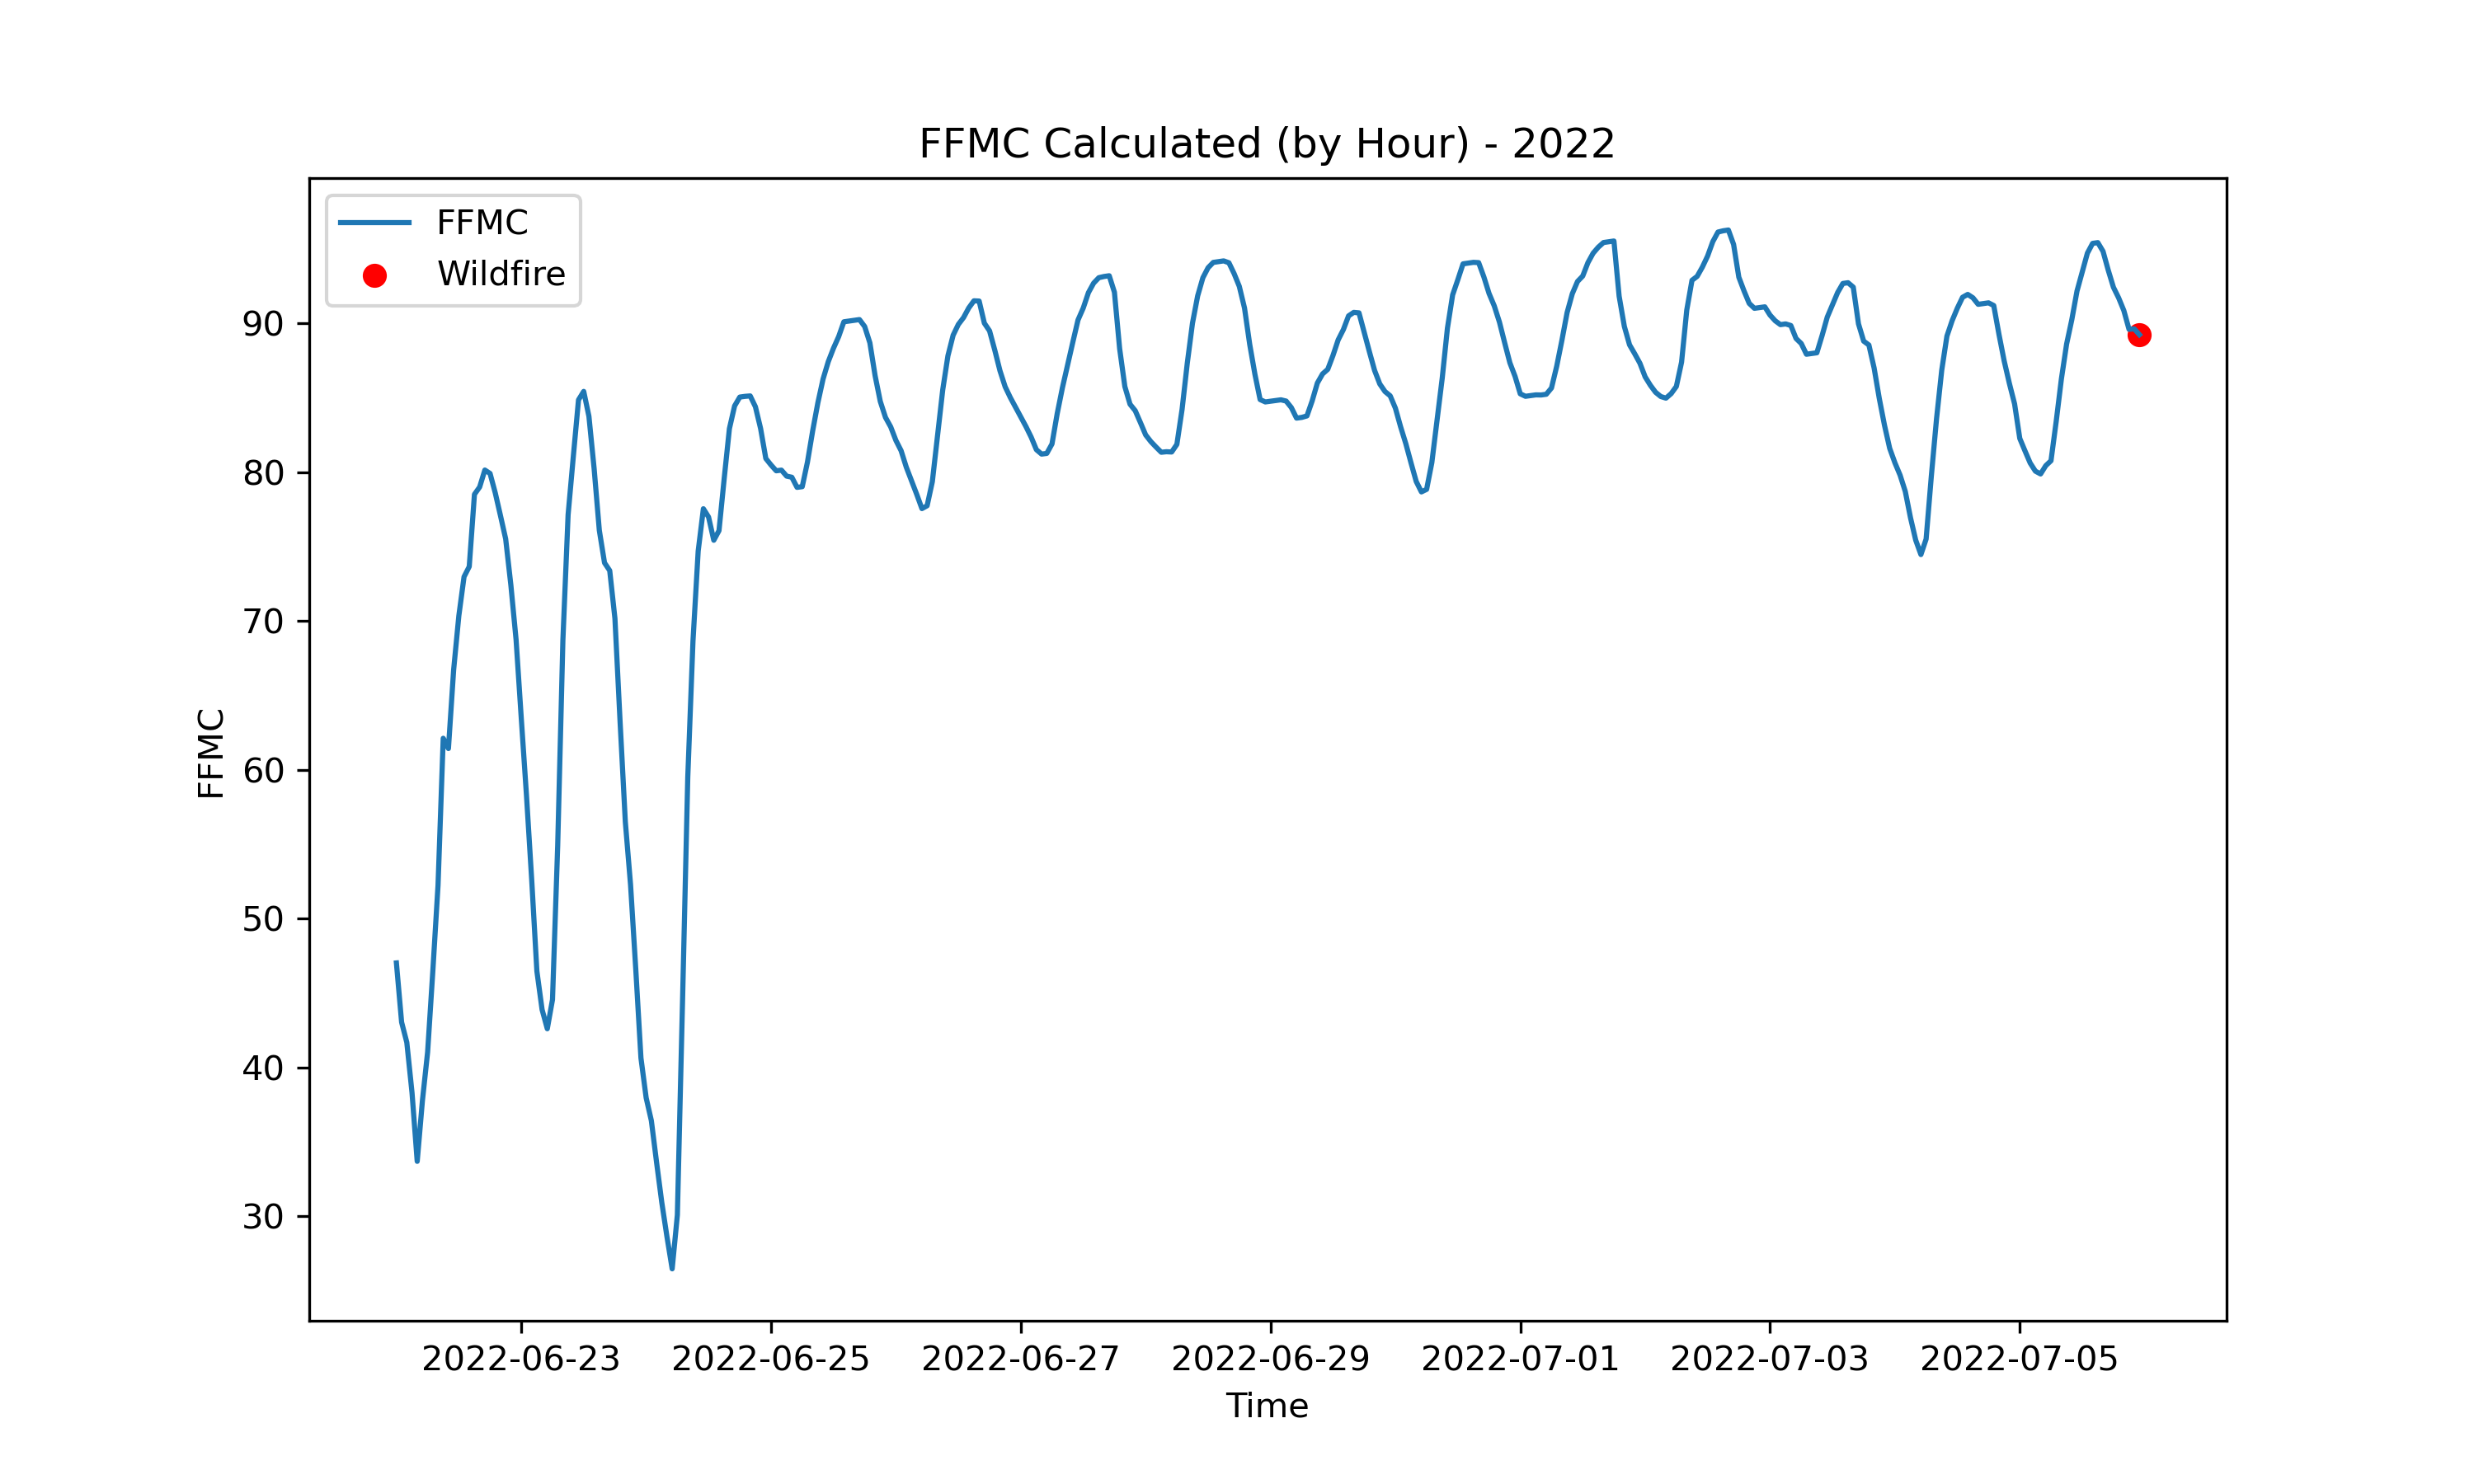
\includegraphics[width=\textwidth]{graphs/2022/2022CalcFFMC12.png}
	\end{subfigure}
	\label{fig:hourly_ffmc}
\end{figure}

\begin{figure}[h]
	\centering
	\caption{Calculated hourly DMC value for 2015, 2019, and 2022}
	\begin{subfigure}{0.45\textwidth}
		\centering
		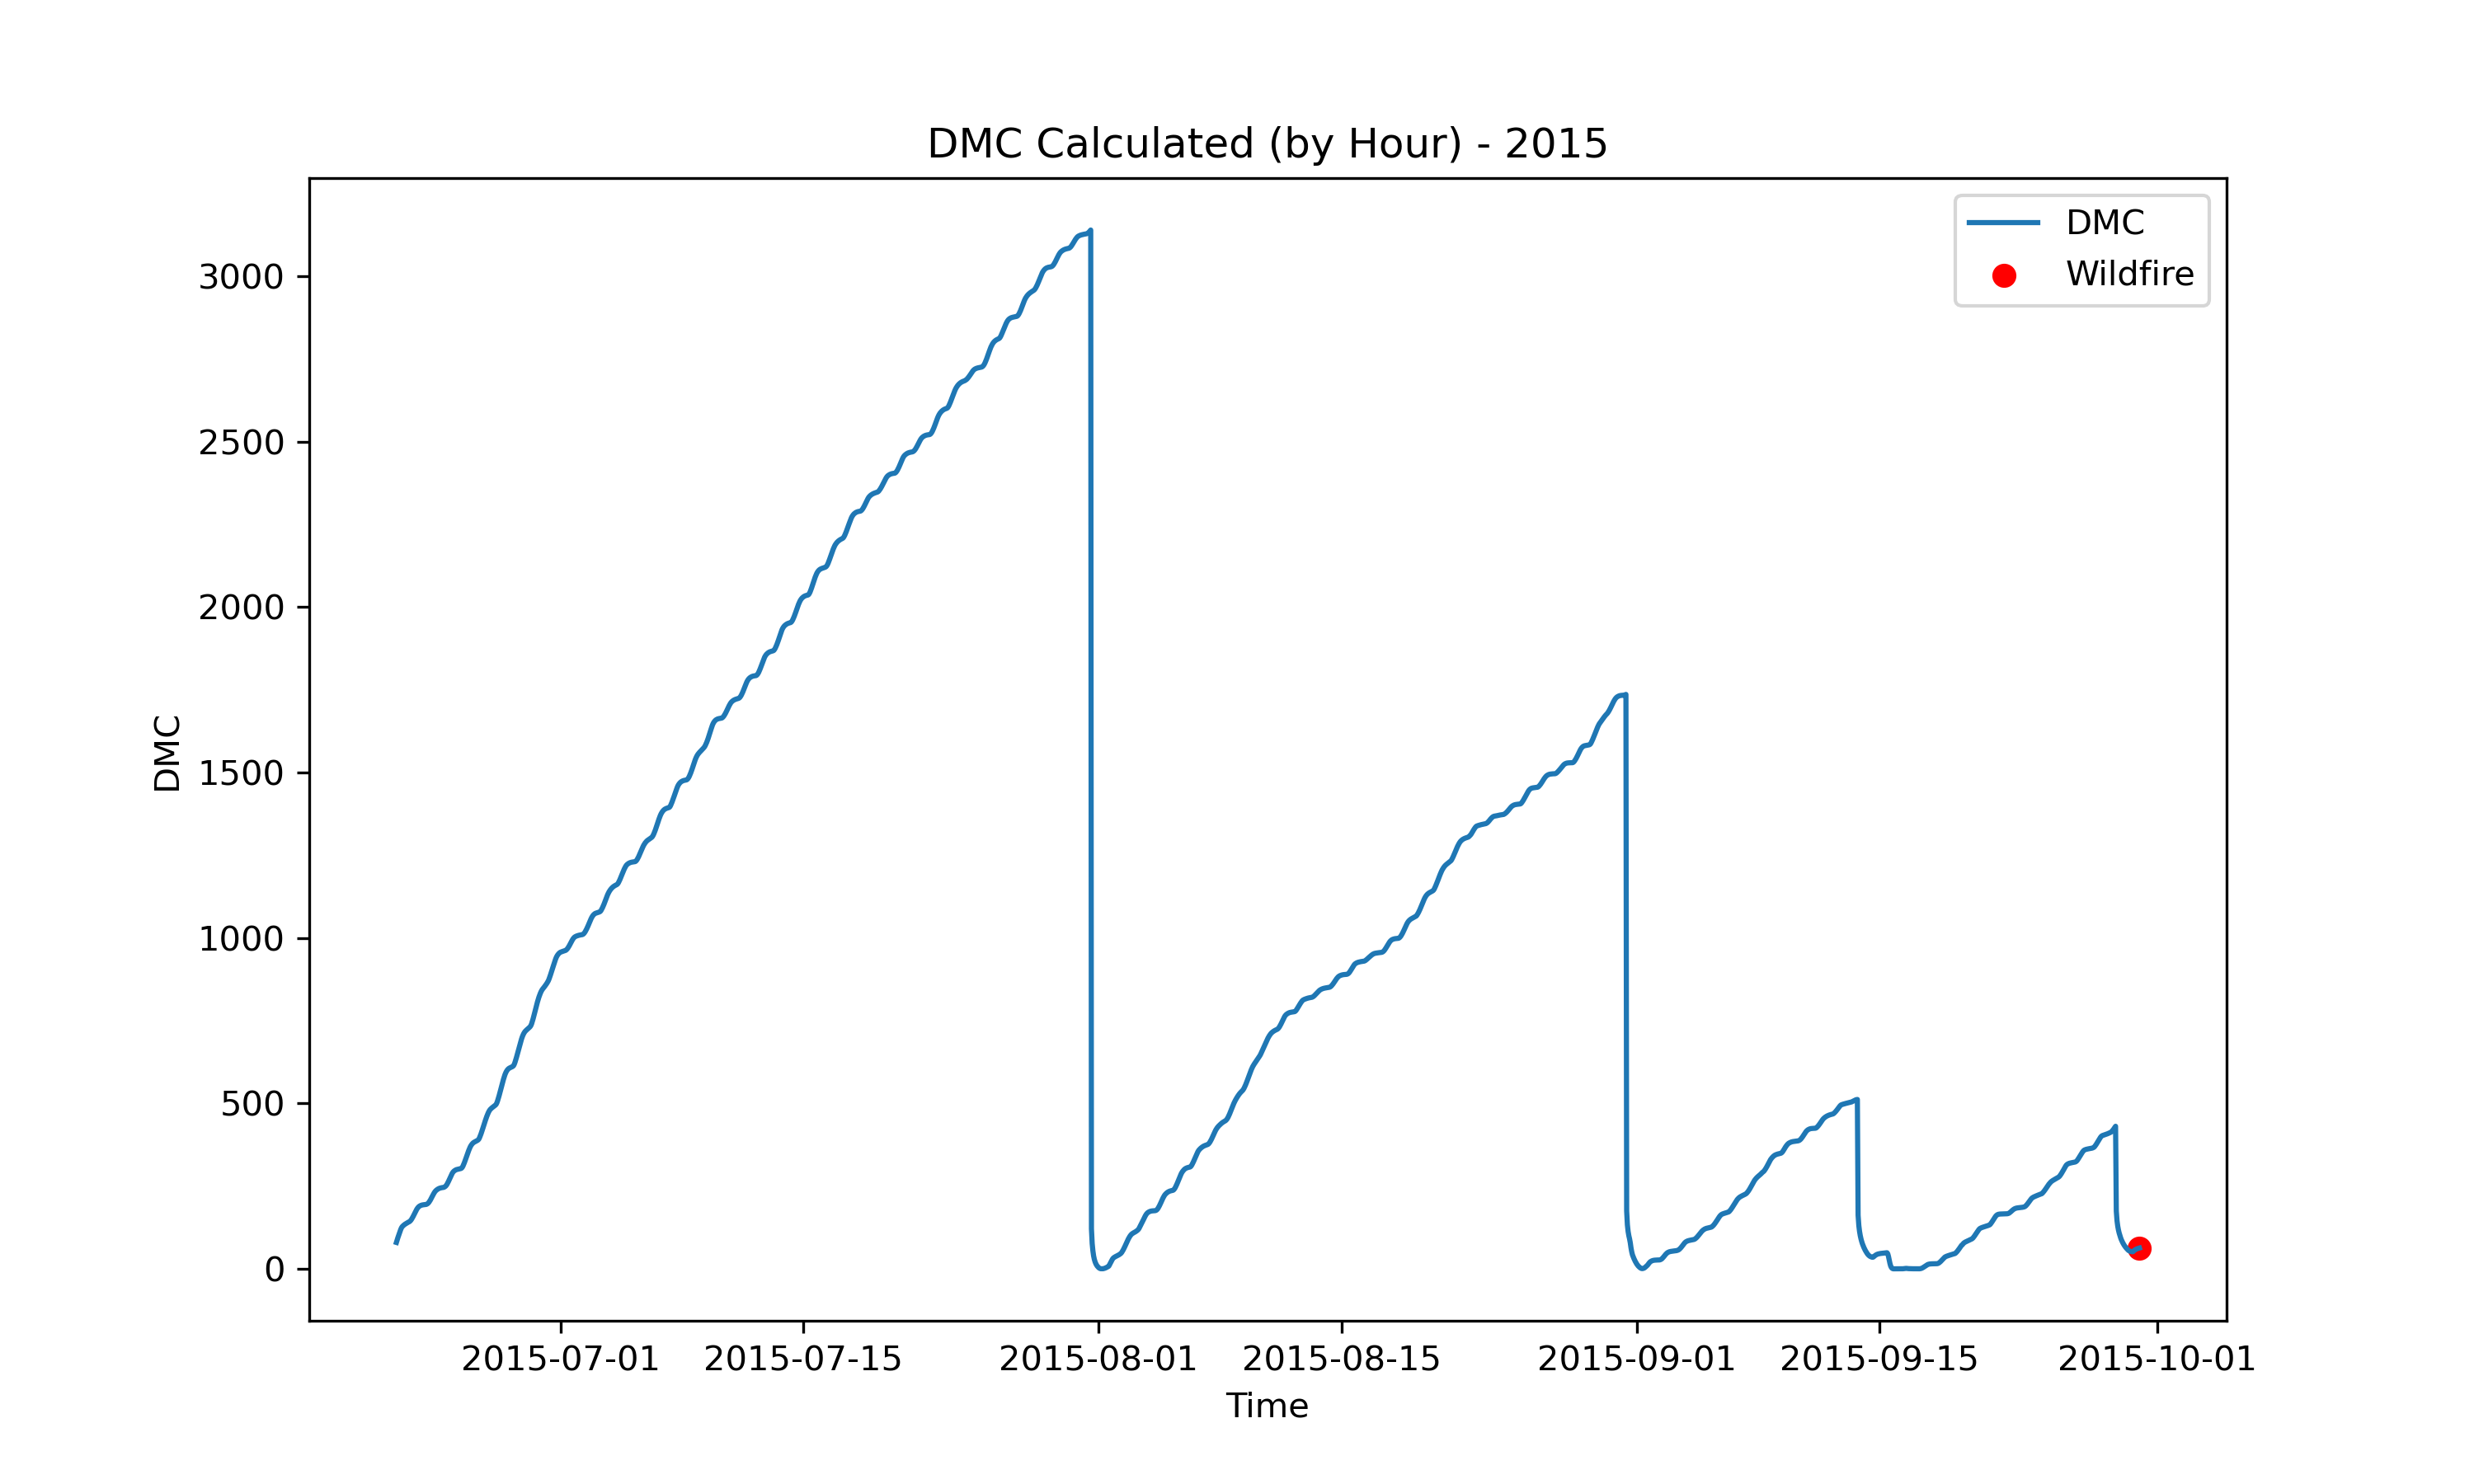
\includegraphics[width=\textwidth]{graphs/2015/byHour/2015CalcDMC12.png}
	\end{subfigure}
	\hfill
	\begin{subfigure}{0.45\textwidth}
		\centering
		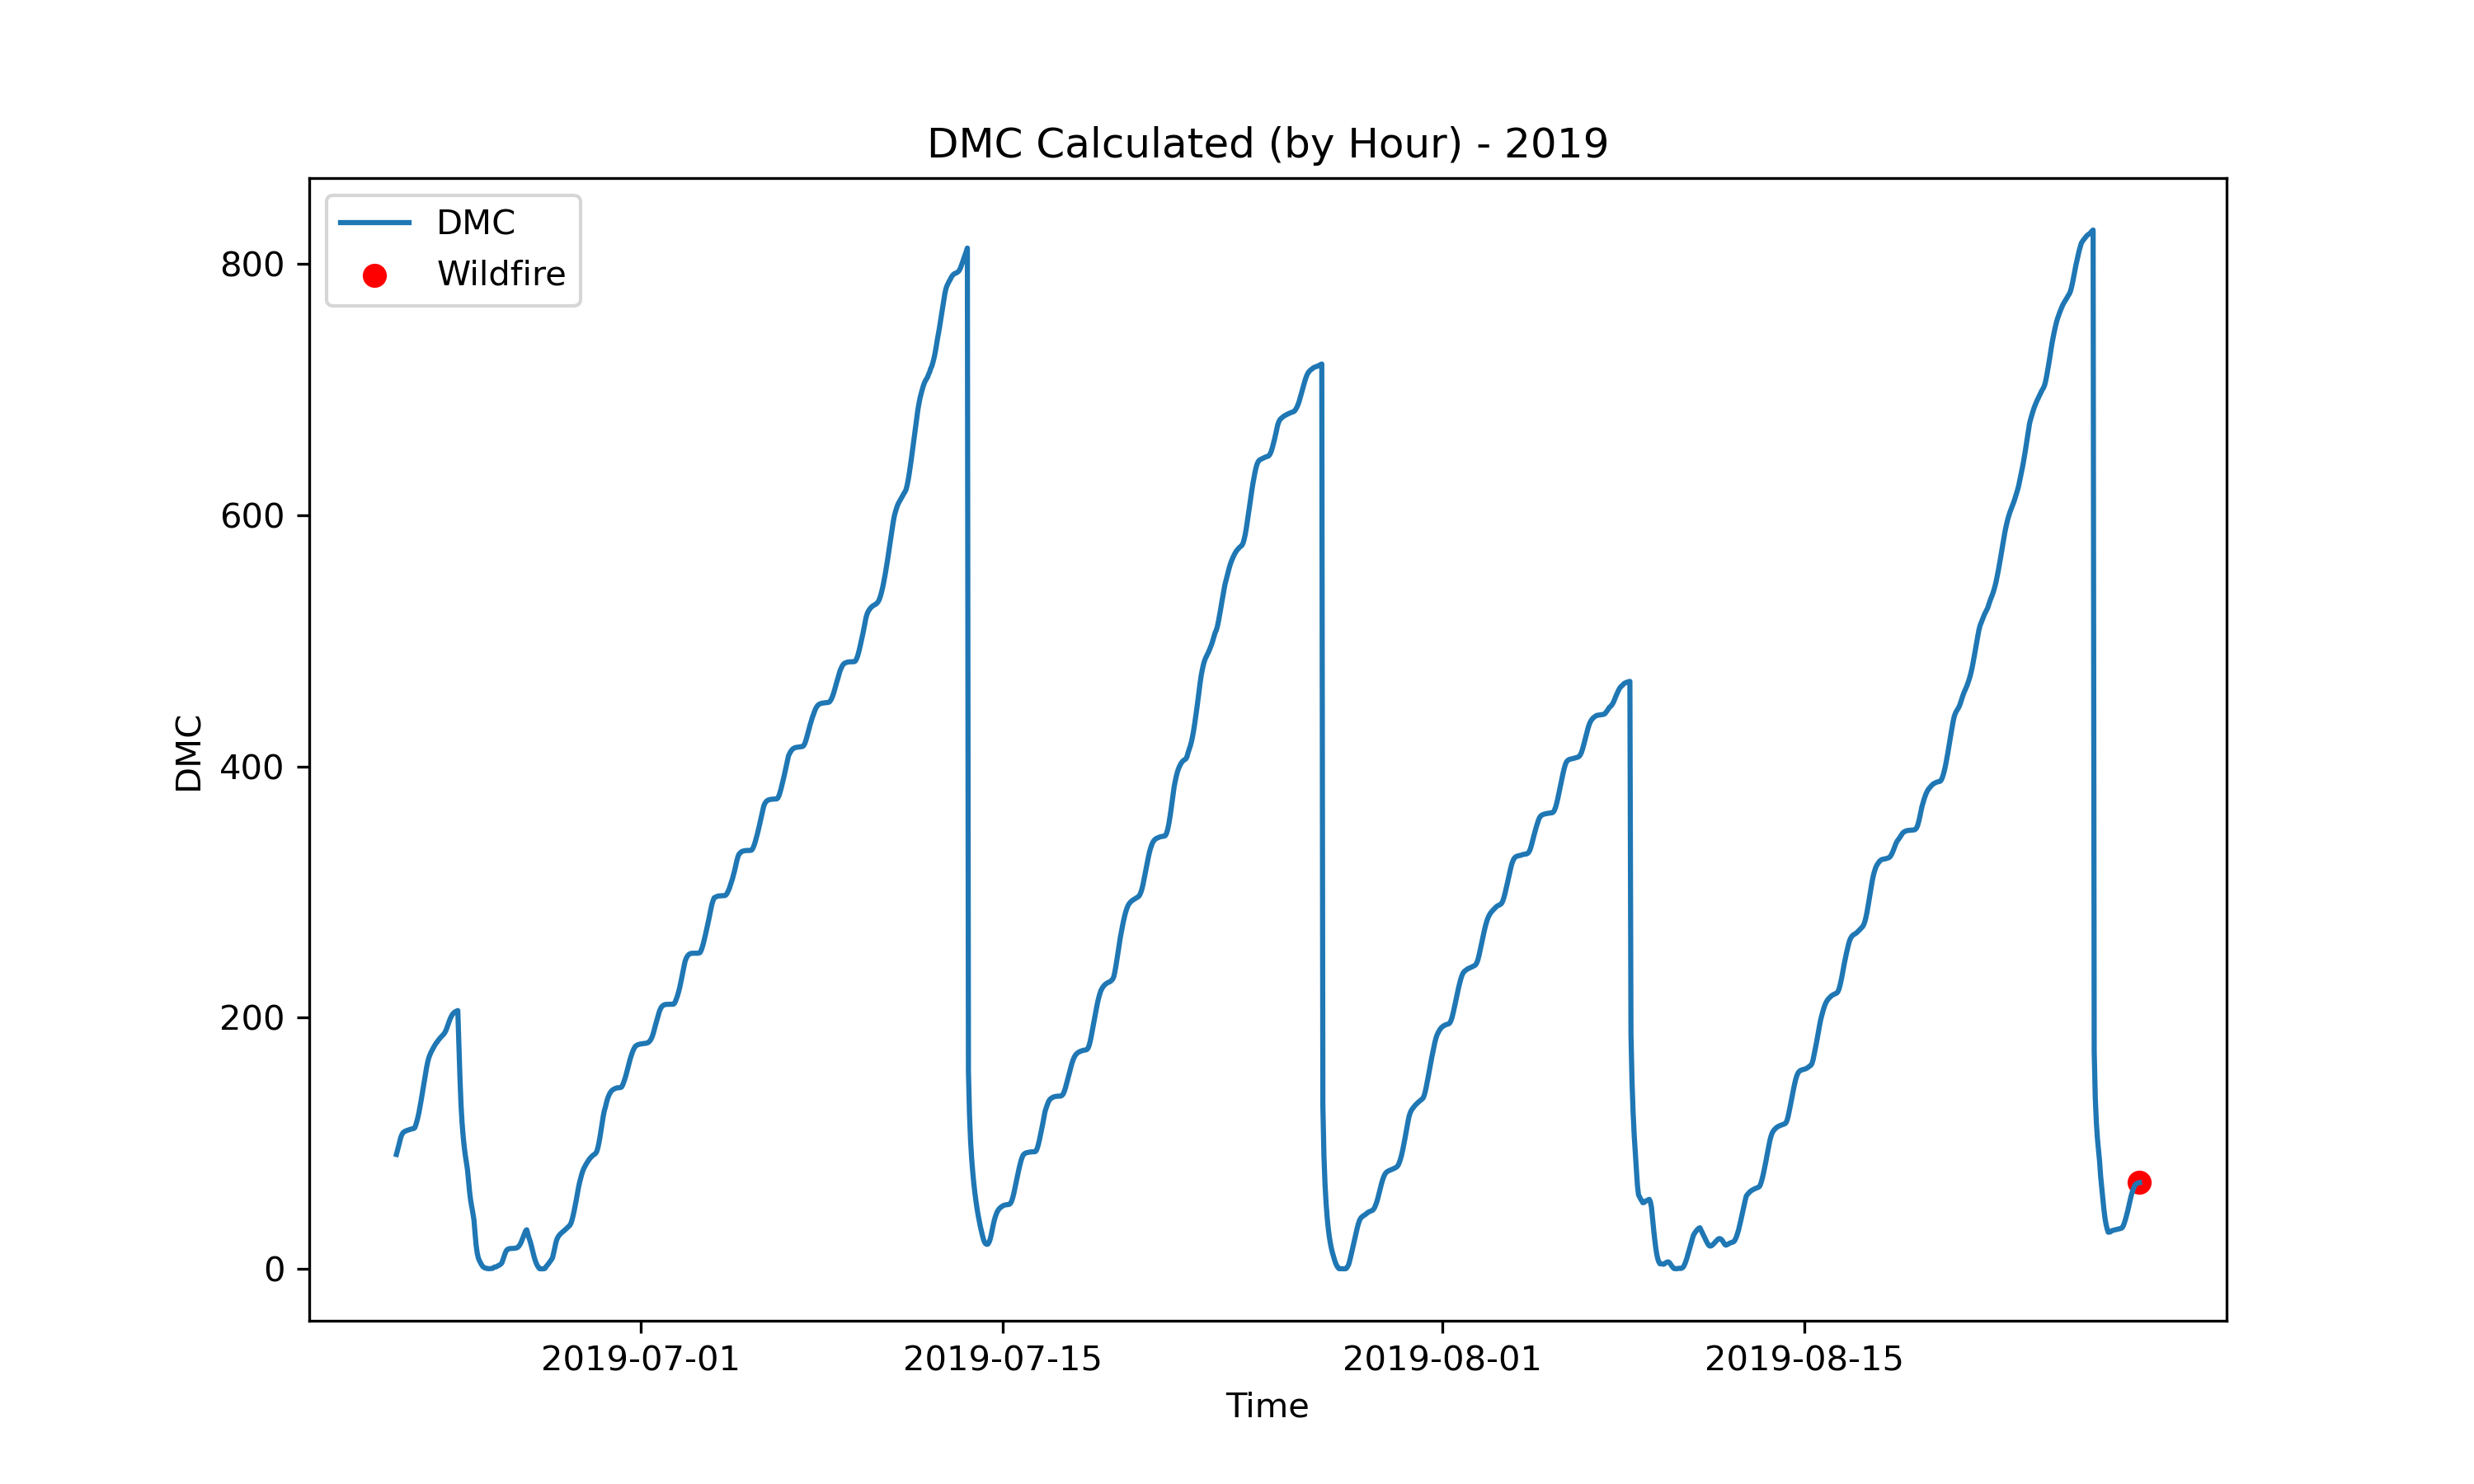
\includegraphics[width=\textwidth]{graphs/2019/2019CalcDMC12.png}
	\end{subfigure}
	\hfill
	\begin{subfigure}{0.45\textwidth}
		\centering
		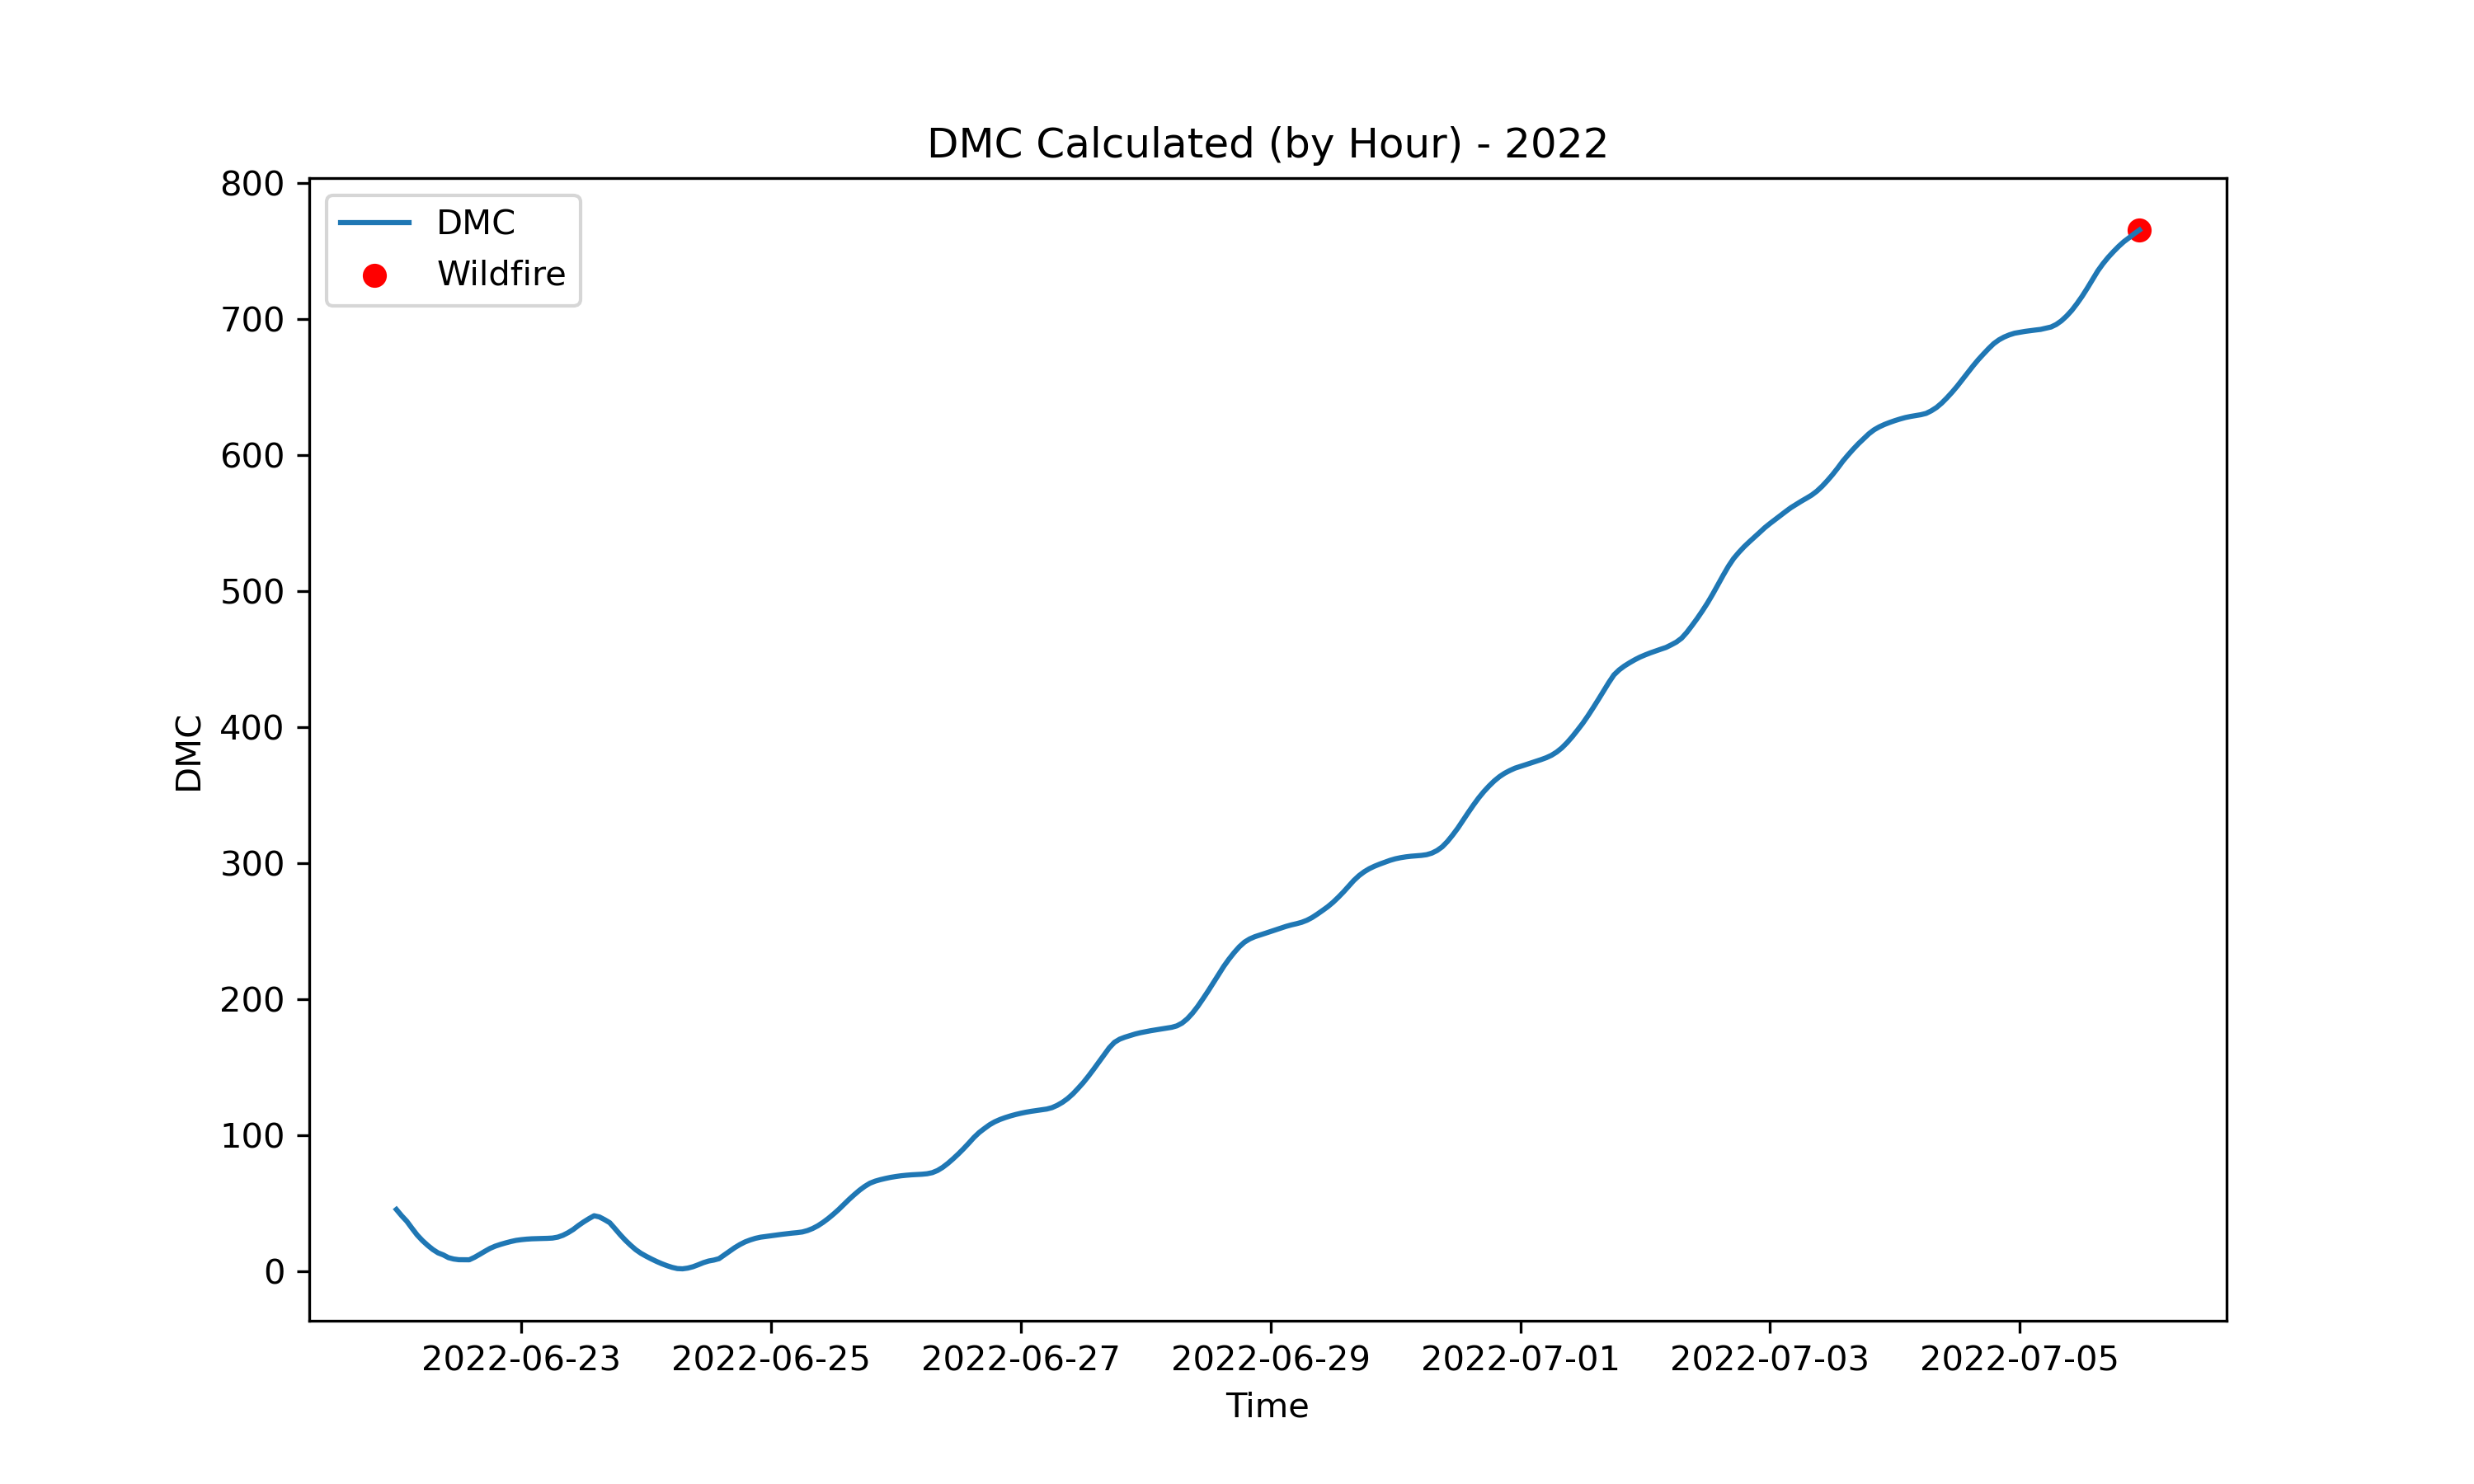
\includegraphics[width=\textwidth]{graphs/2022/2022CalcDMC12.png}
	\end{subfigure}
	
	\label{fig:hourly_dmc}
\end{figure}

\begin{figure}[h]
	\centering
	\caption{Calculated hourly DC value for 2015, 2019, and 2022}
	\begin{subfigure}{0.45\textwidth}
		\centering
		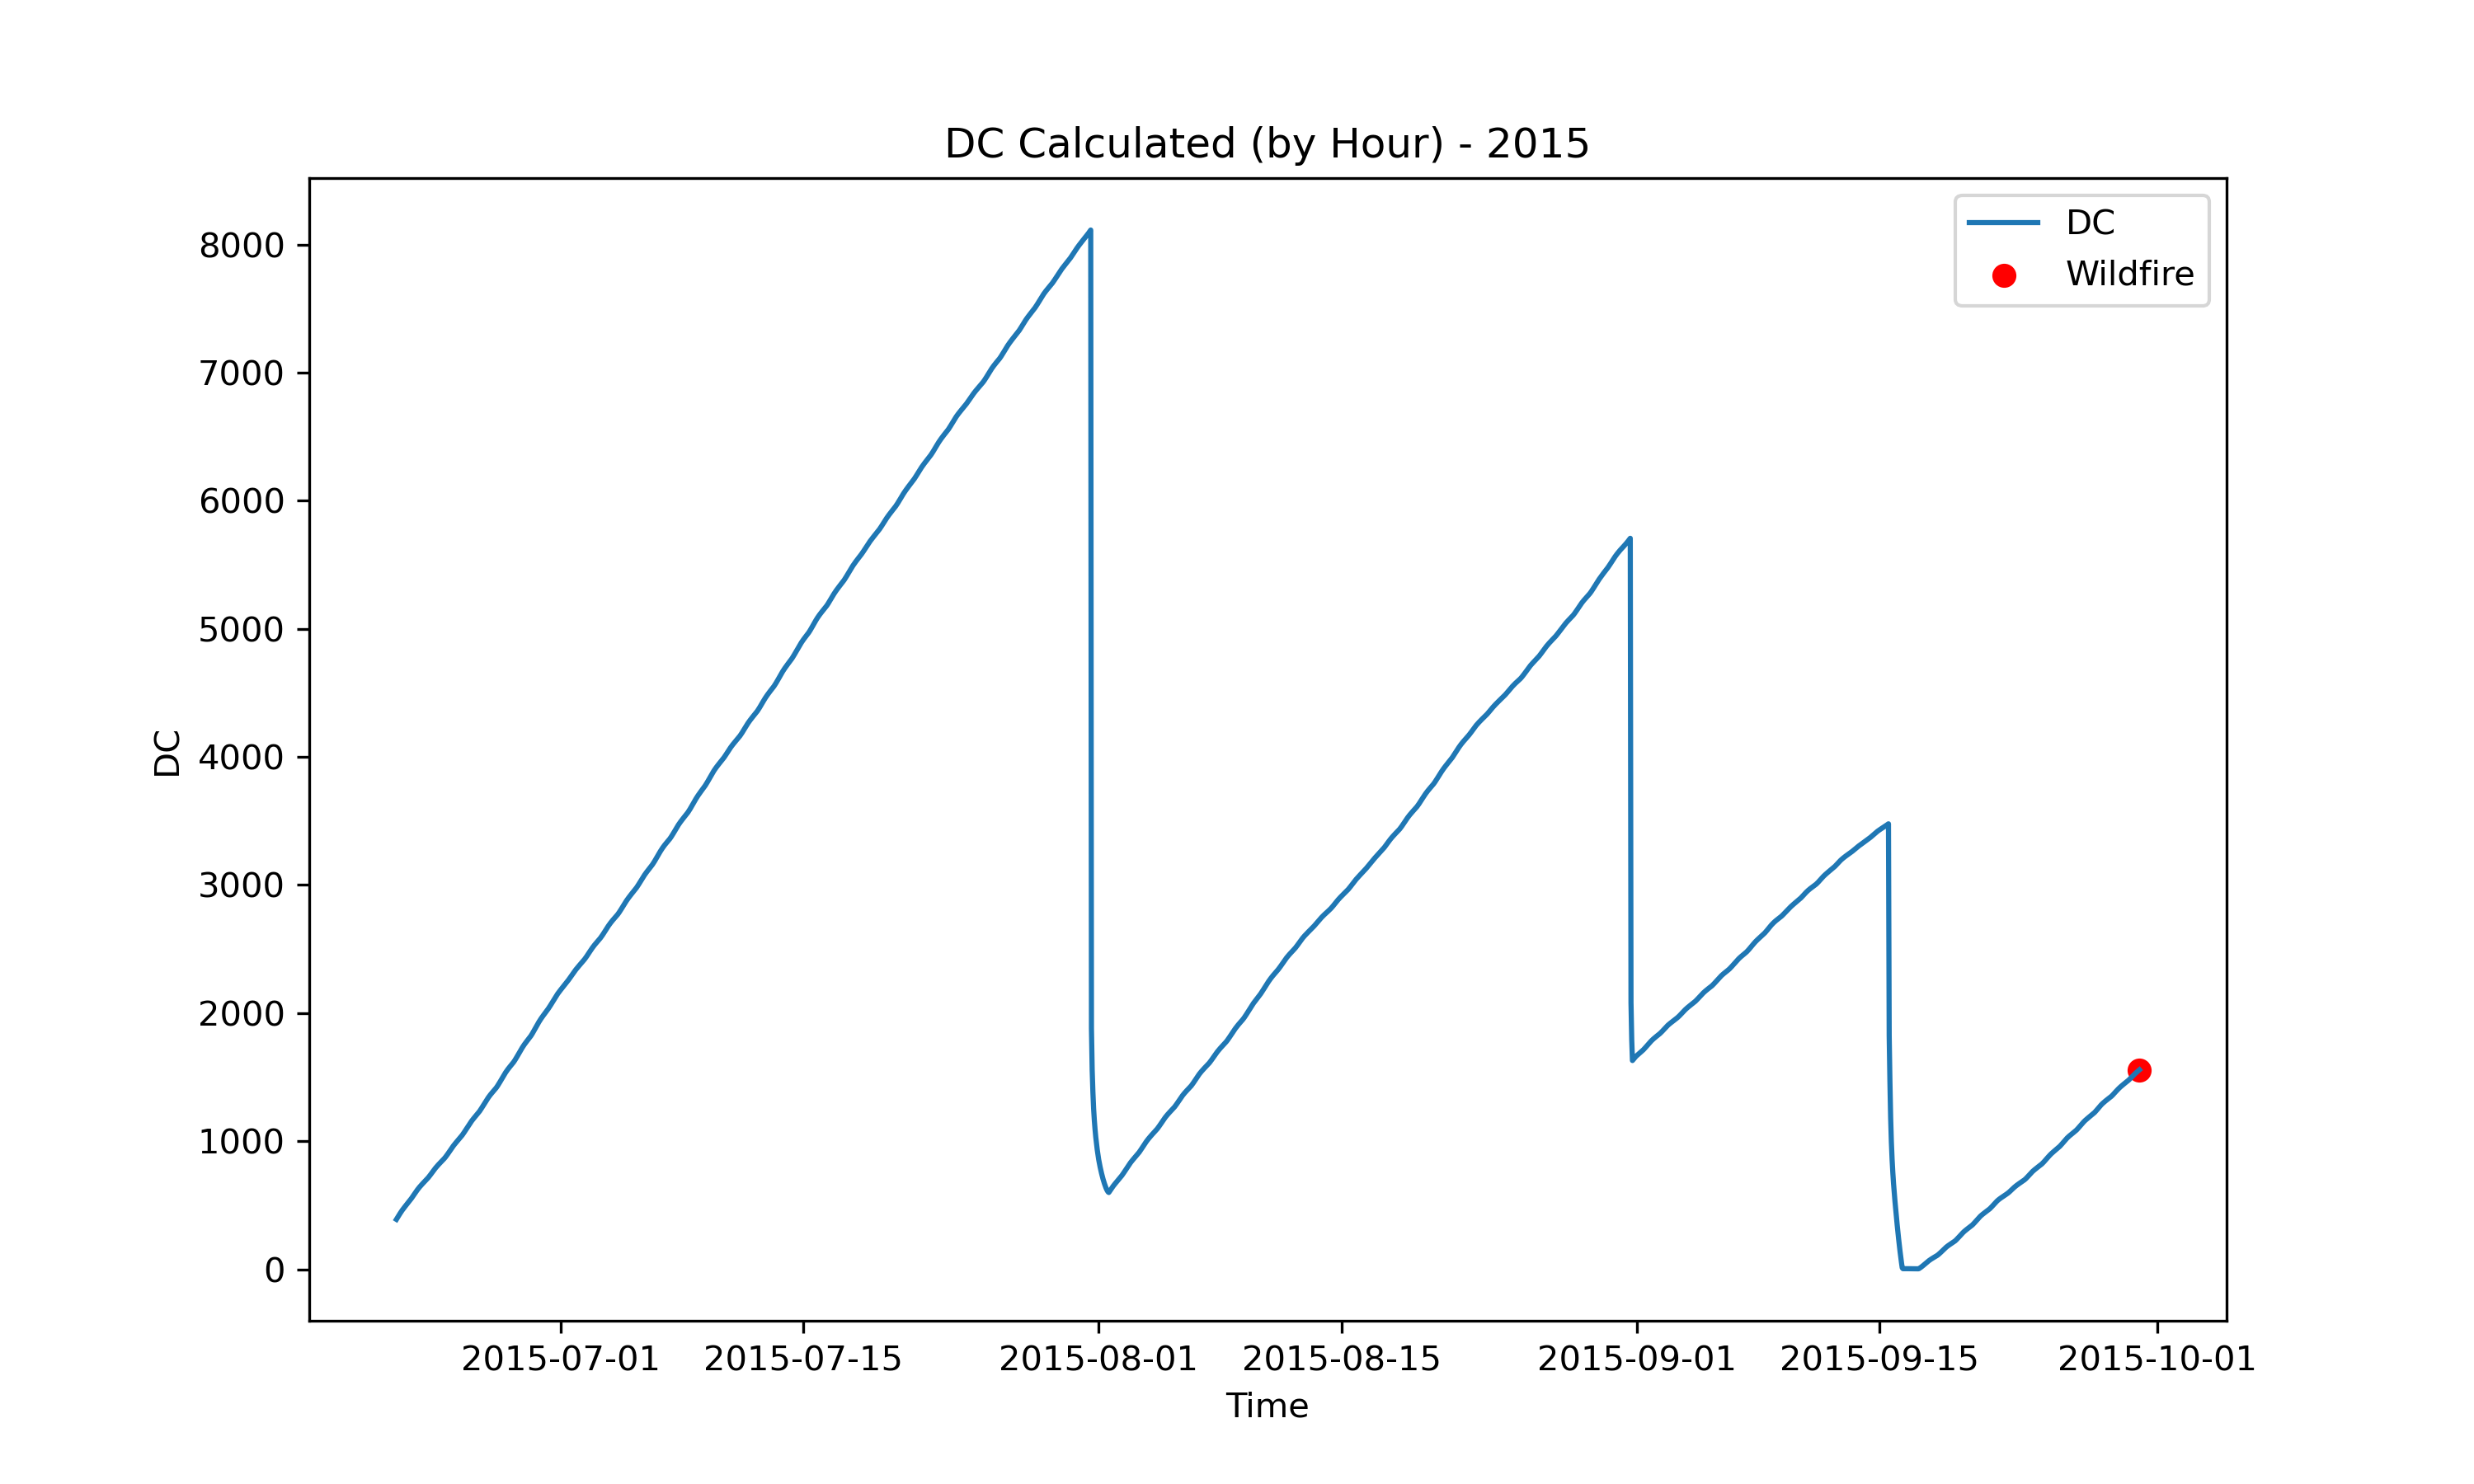
\includegraphics[width=\textwidth]{graphs/2015/byHour/2015CalcDC12.png}
	\end{subfigure}
	\hfill
	\begin{subfigure}{0.45\textwidth}
		\centering
		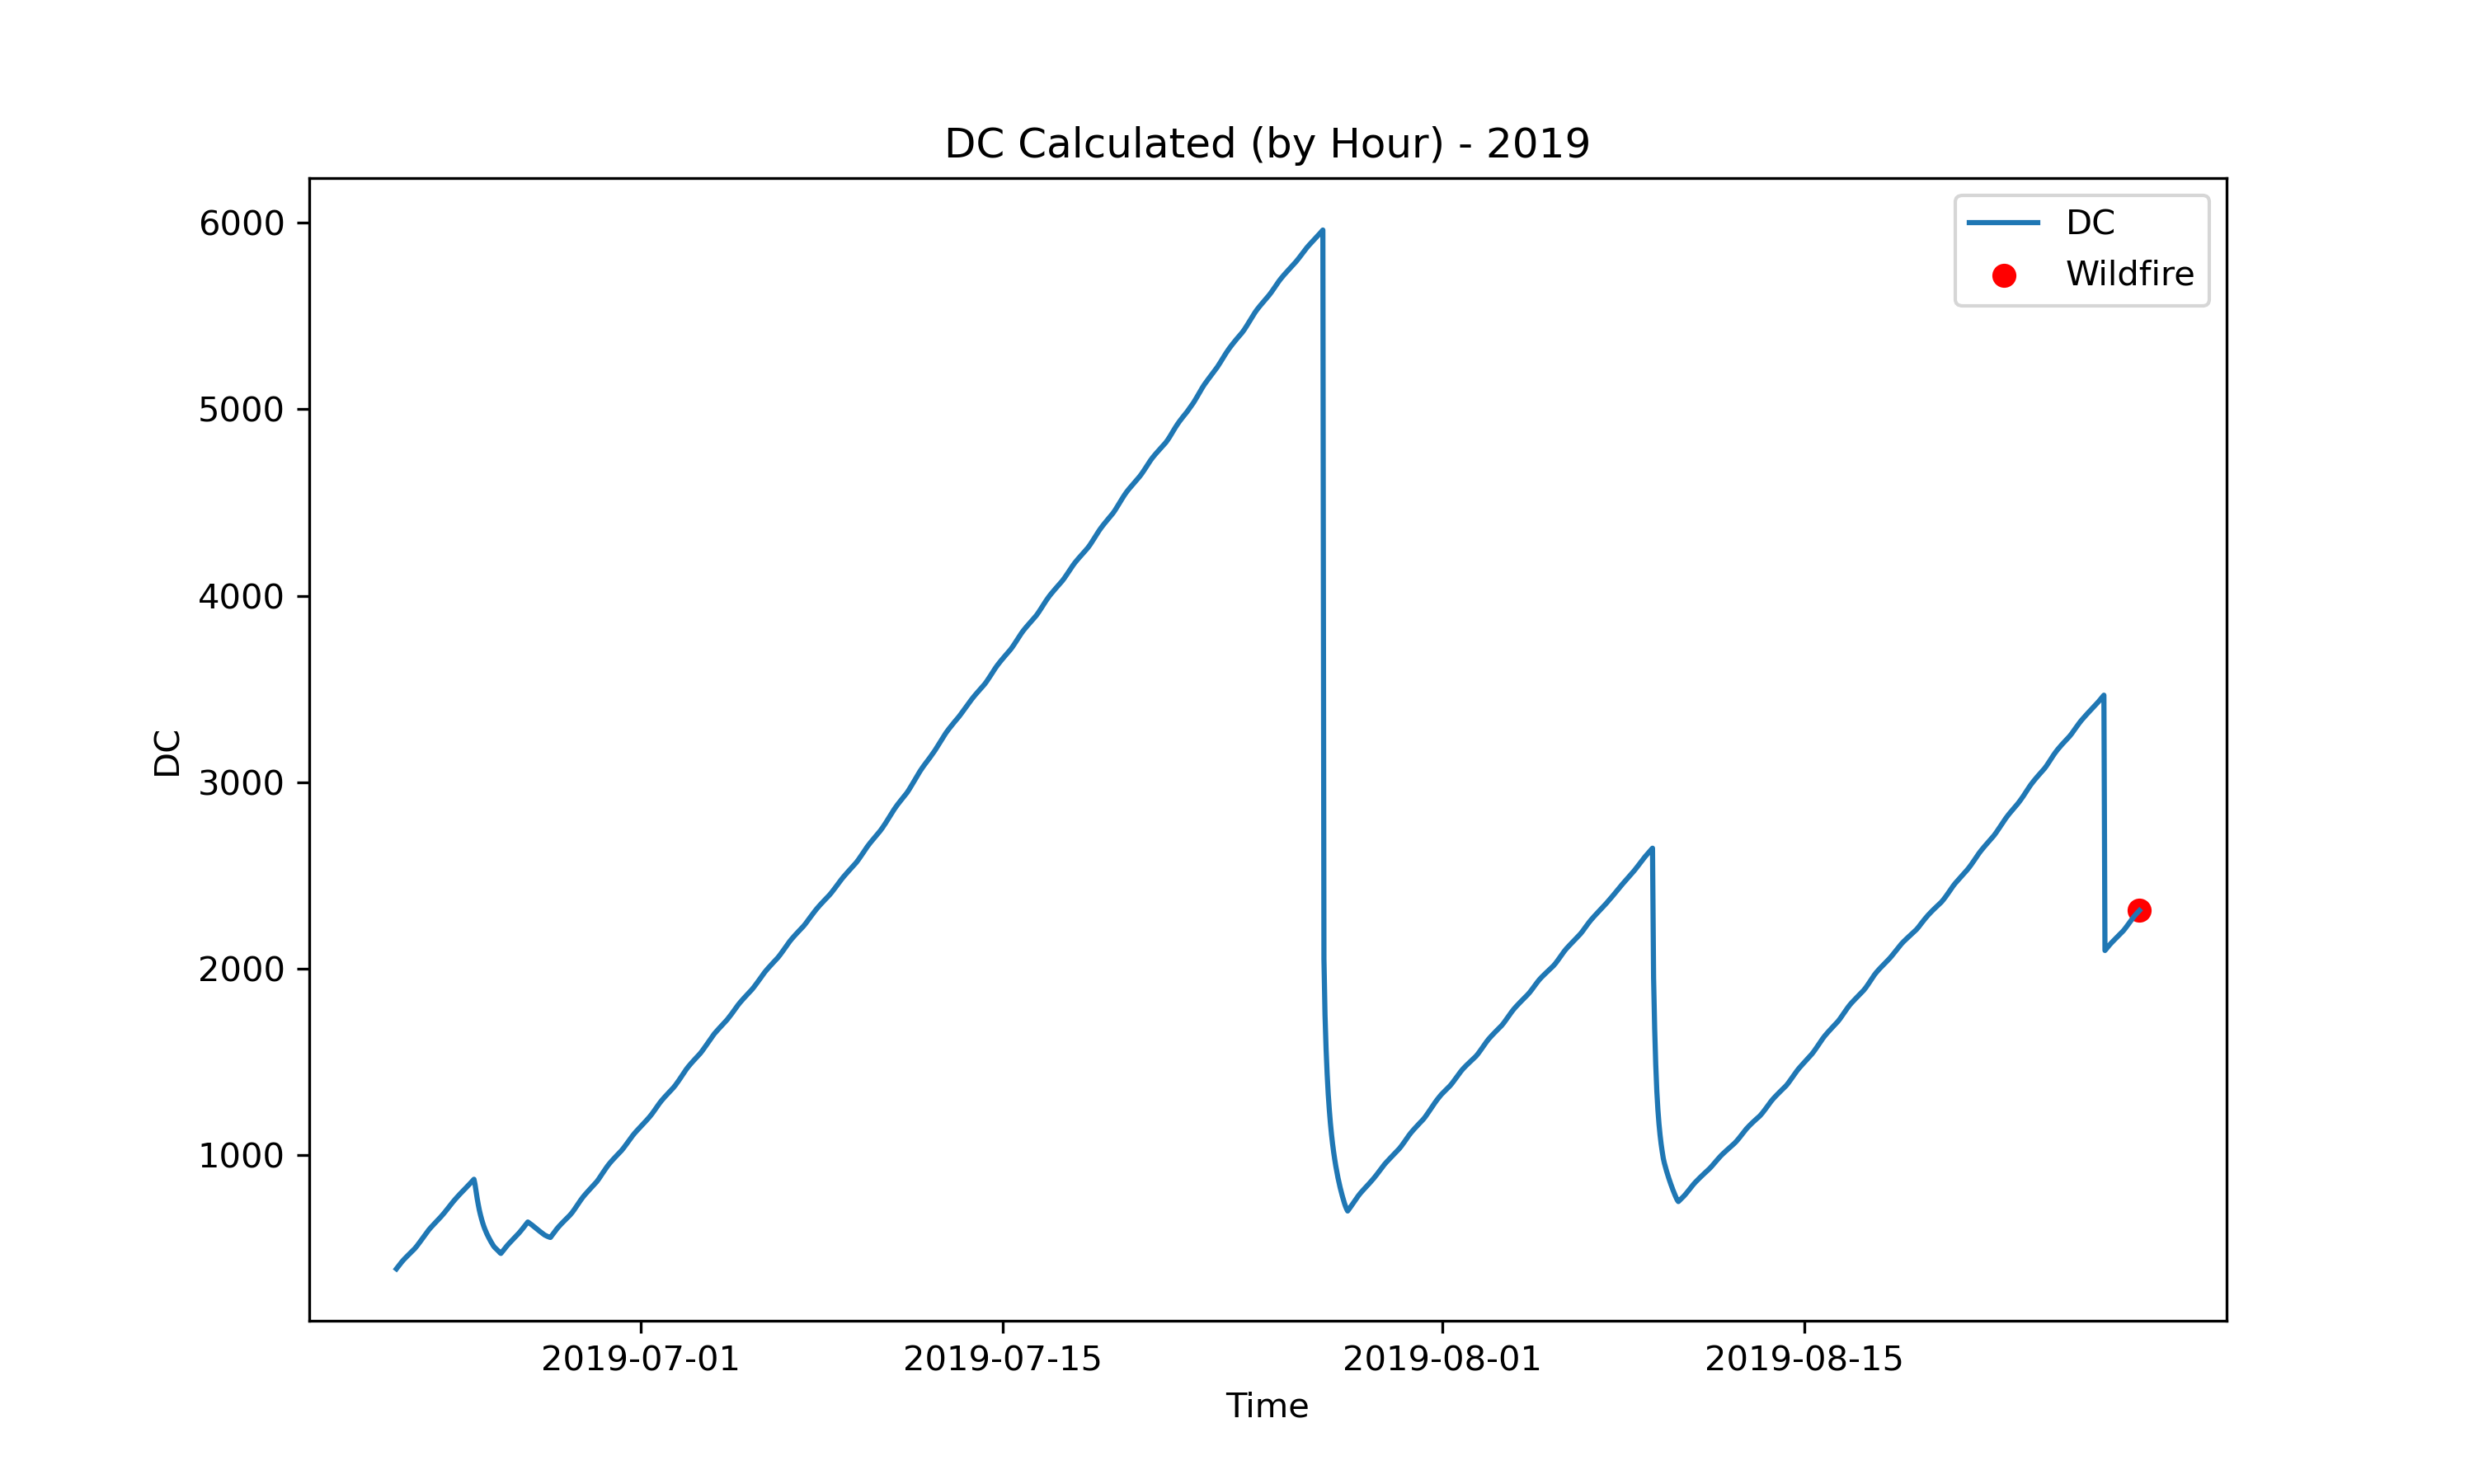
\includegraphics[width=\textwidth]{graphs/2019/2019CalcDC12.png}
	\end{subfigure}
	\hfill
	\begin{subfigure}{0.45\textwidth}
		\centering
		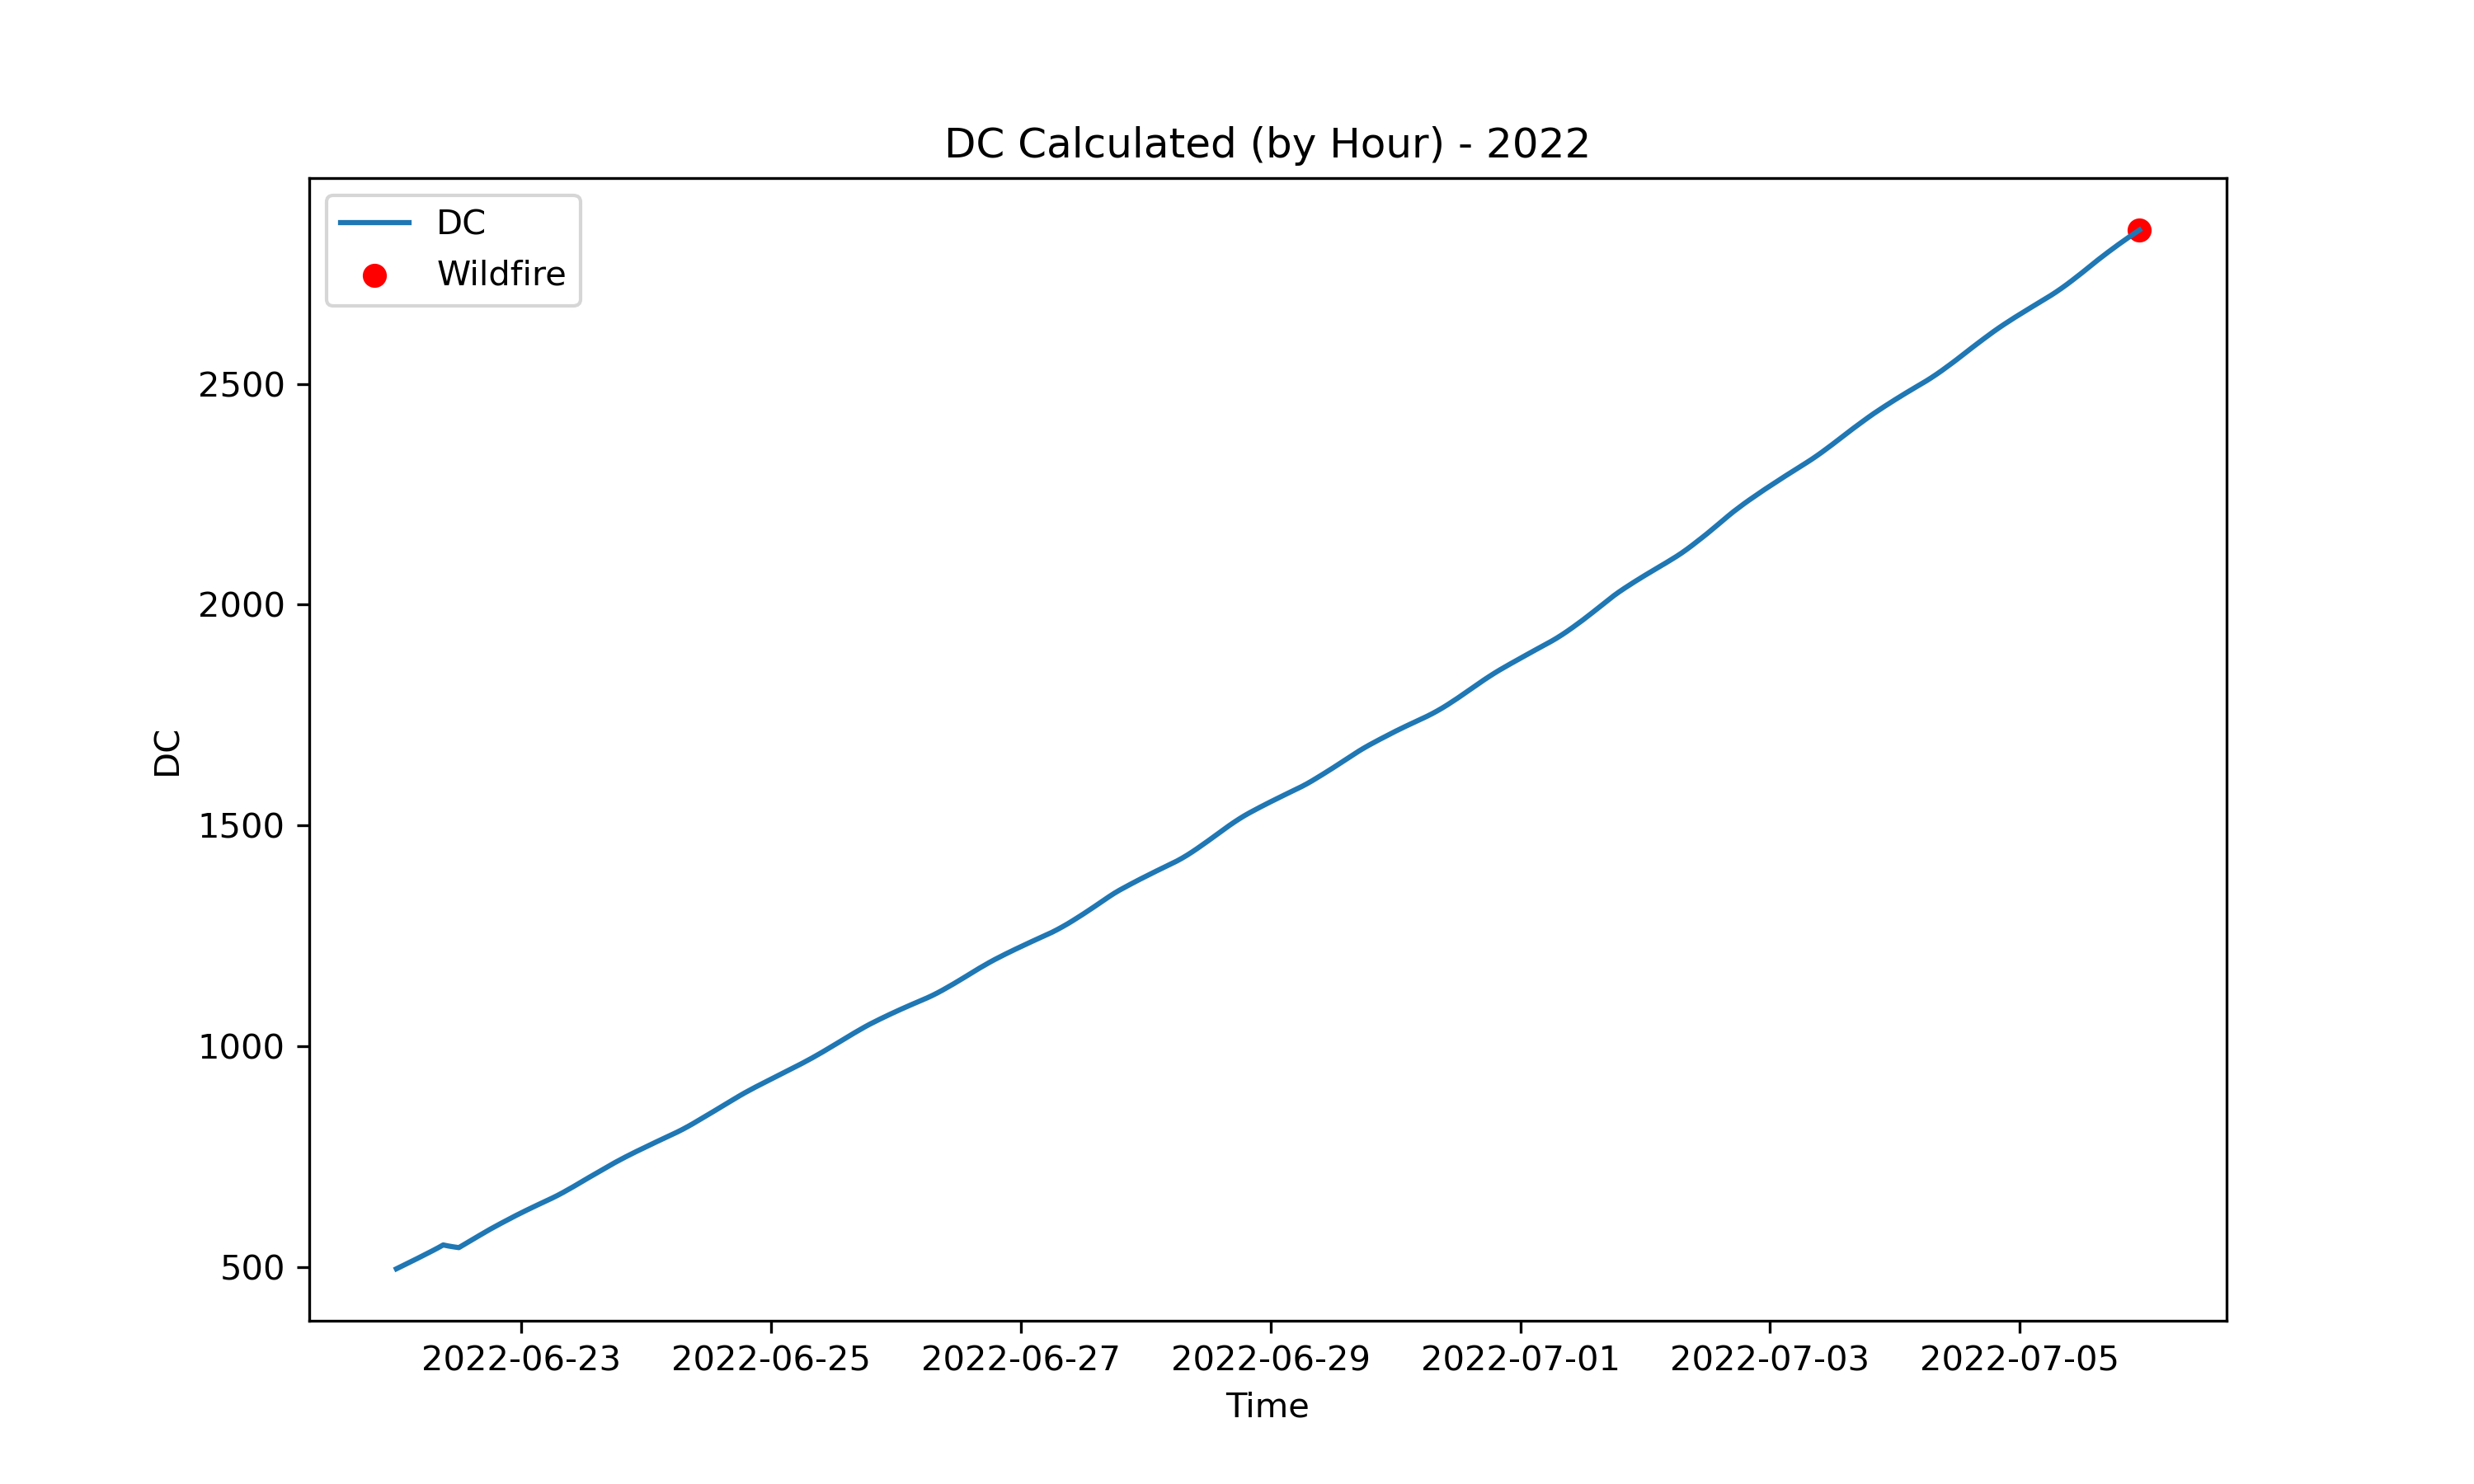
\includegraphics[width=\textwidth]{graphs/2022/2022CalcDC12.png}
	\end{subfigure}
	\label{fig:hourly_dc}
\end{figure}

\begin{figure}[h]
	\centering
	\caption{Calculated hourly ISI value for 2015, 2019, and 2022}
	\begin{subfigure}{0.45\textwidth}
		\centering
		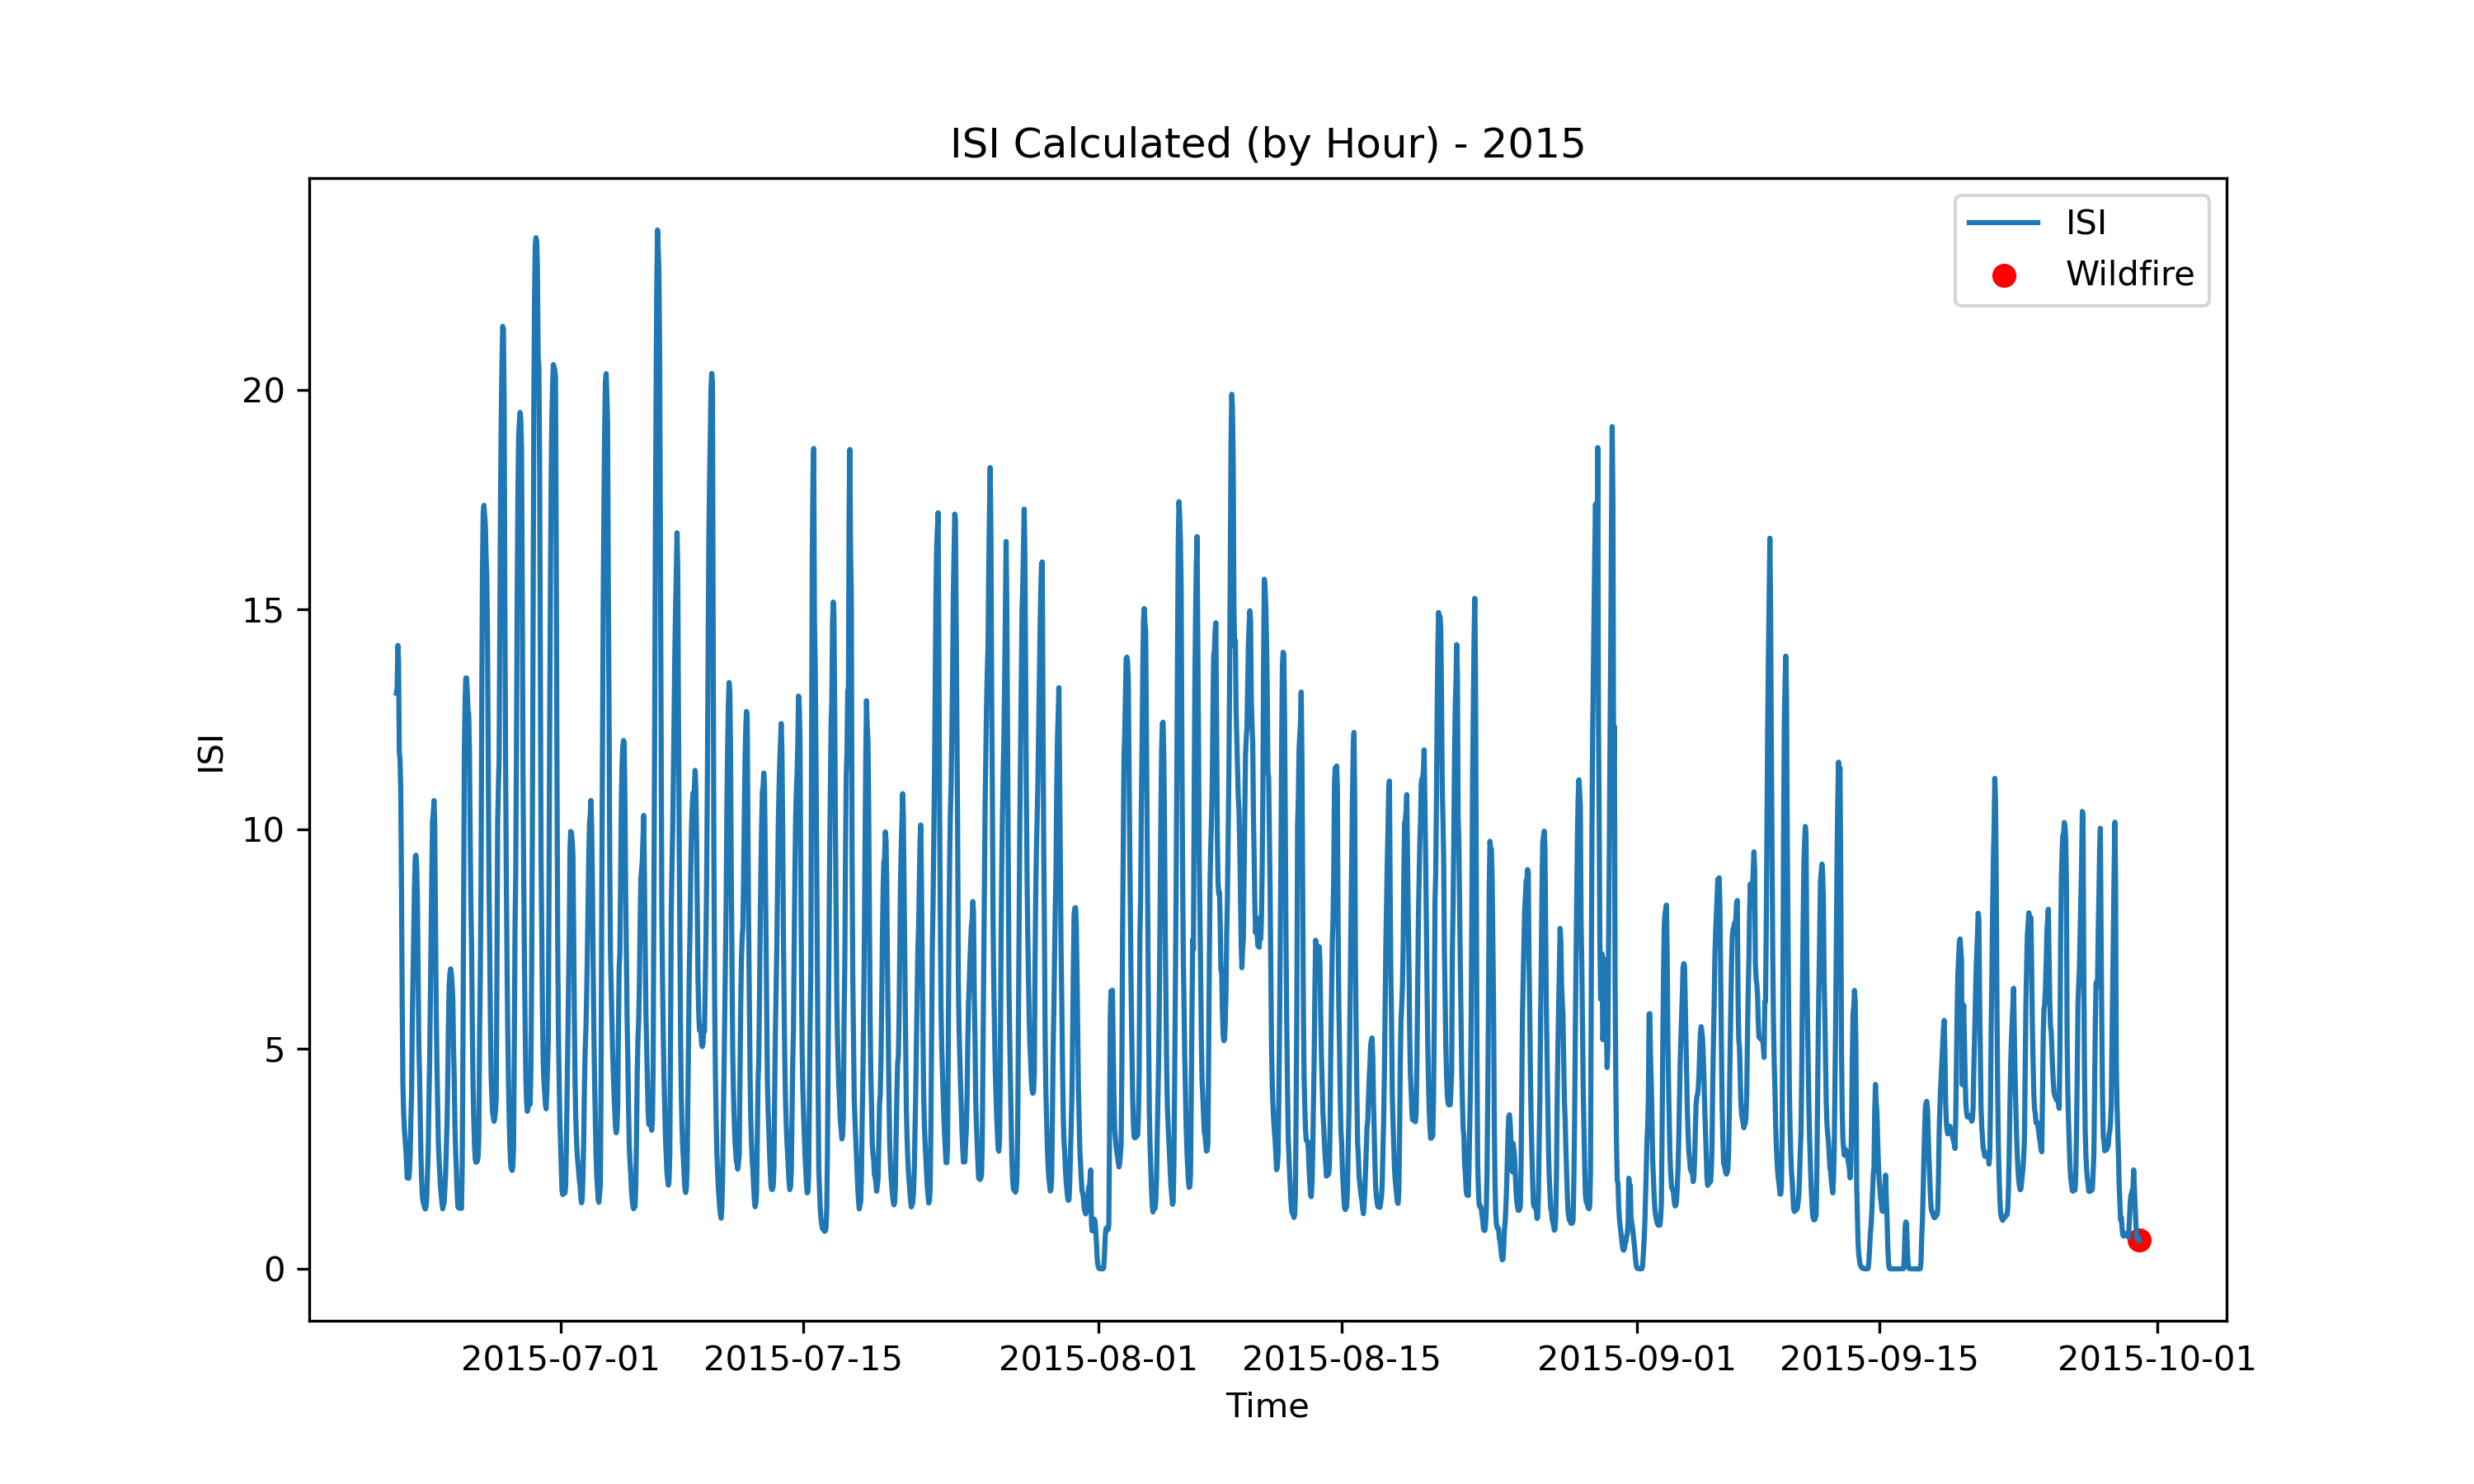
\includegraphics[width=\textwidth]{graphs/2015/byHour/2015CalcISI12.png}
	\end{subfigure}
	\hfill
	\begin{subfigure}{0.45\textwidth}
		\centering
		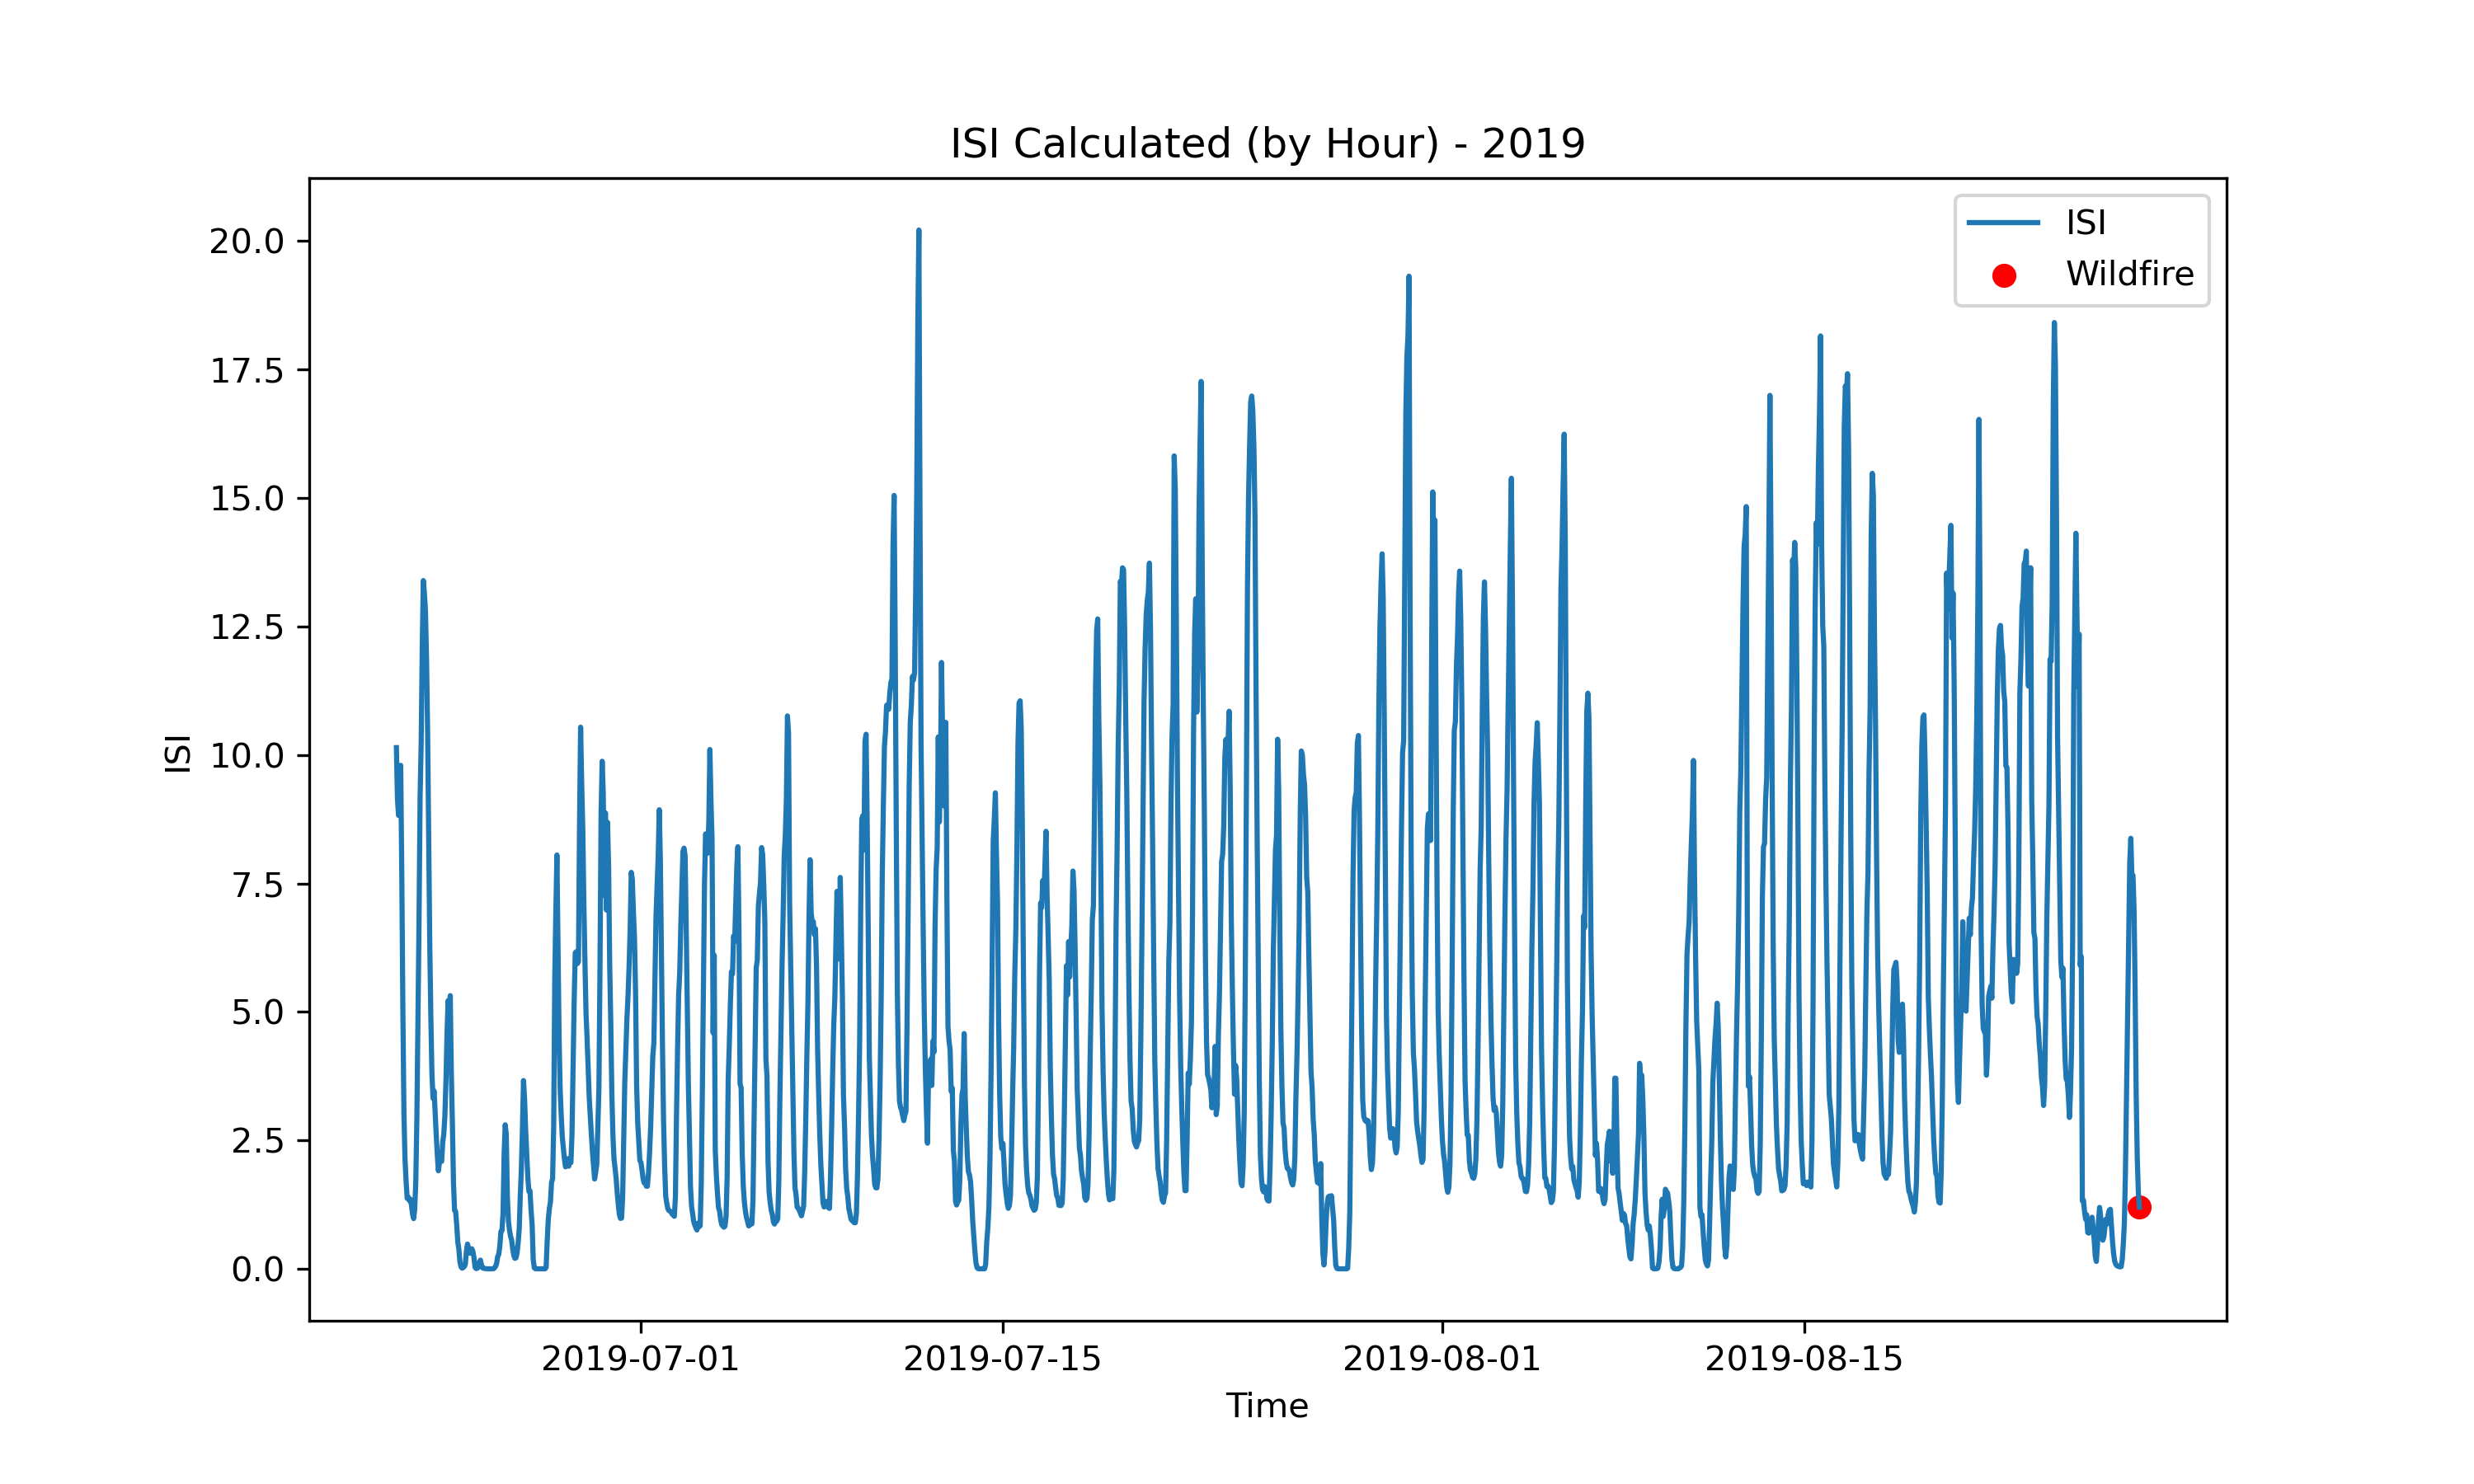
\includegraphics[width=\textwidth]{graphs/2019/2019CalcISI12.png}
	\end{subfigure}
	\hfill
	\begin{subfigure}{0.45\textwidth}
		\centering
		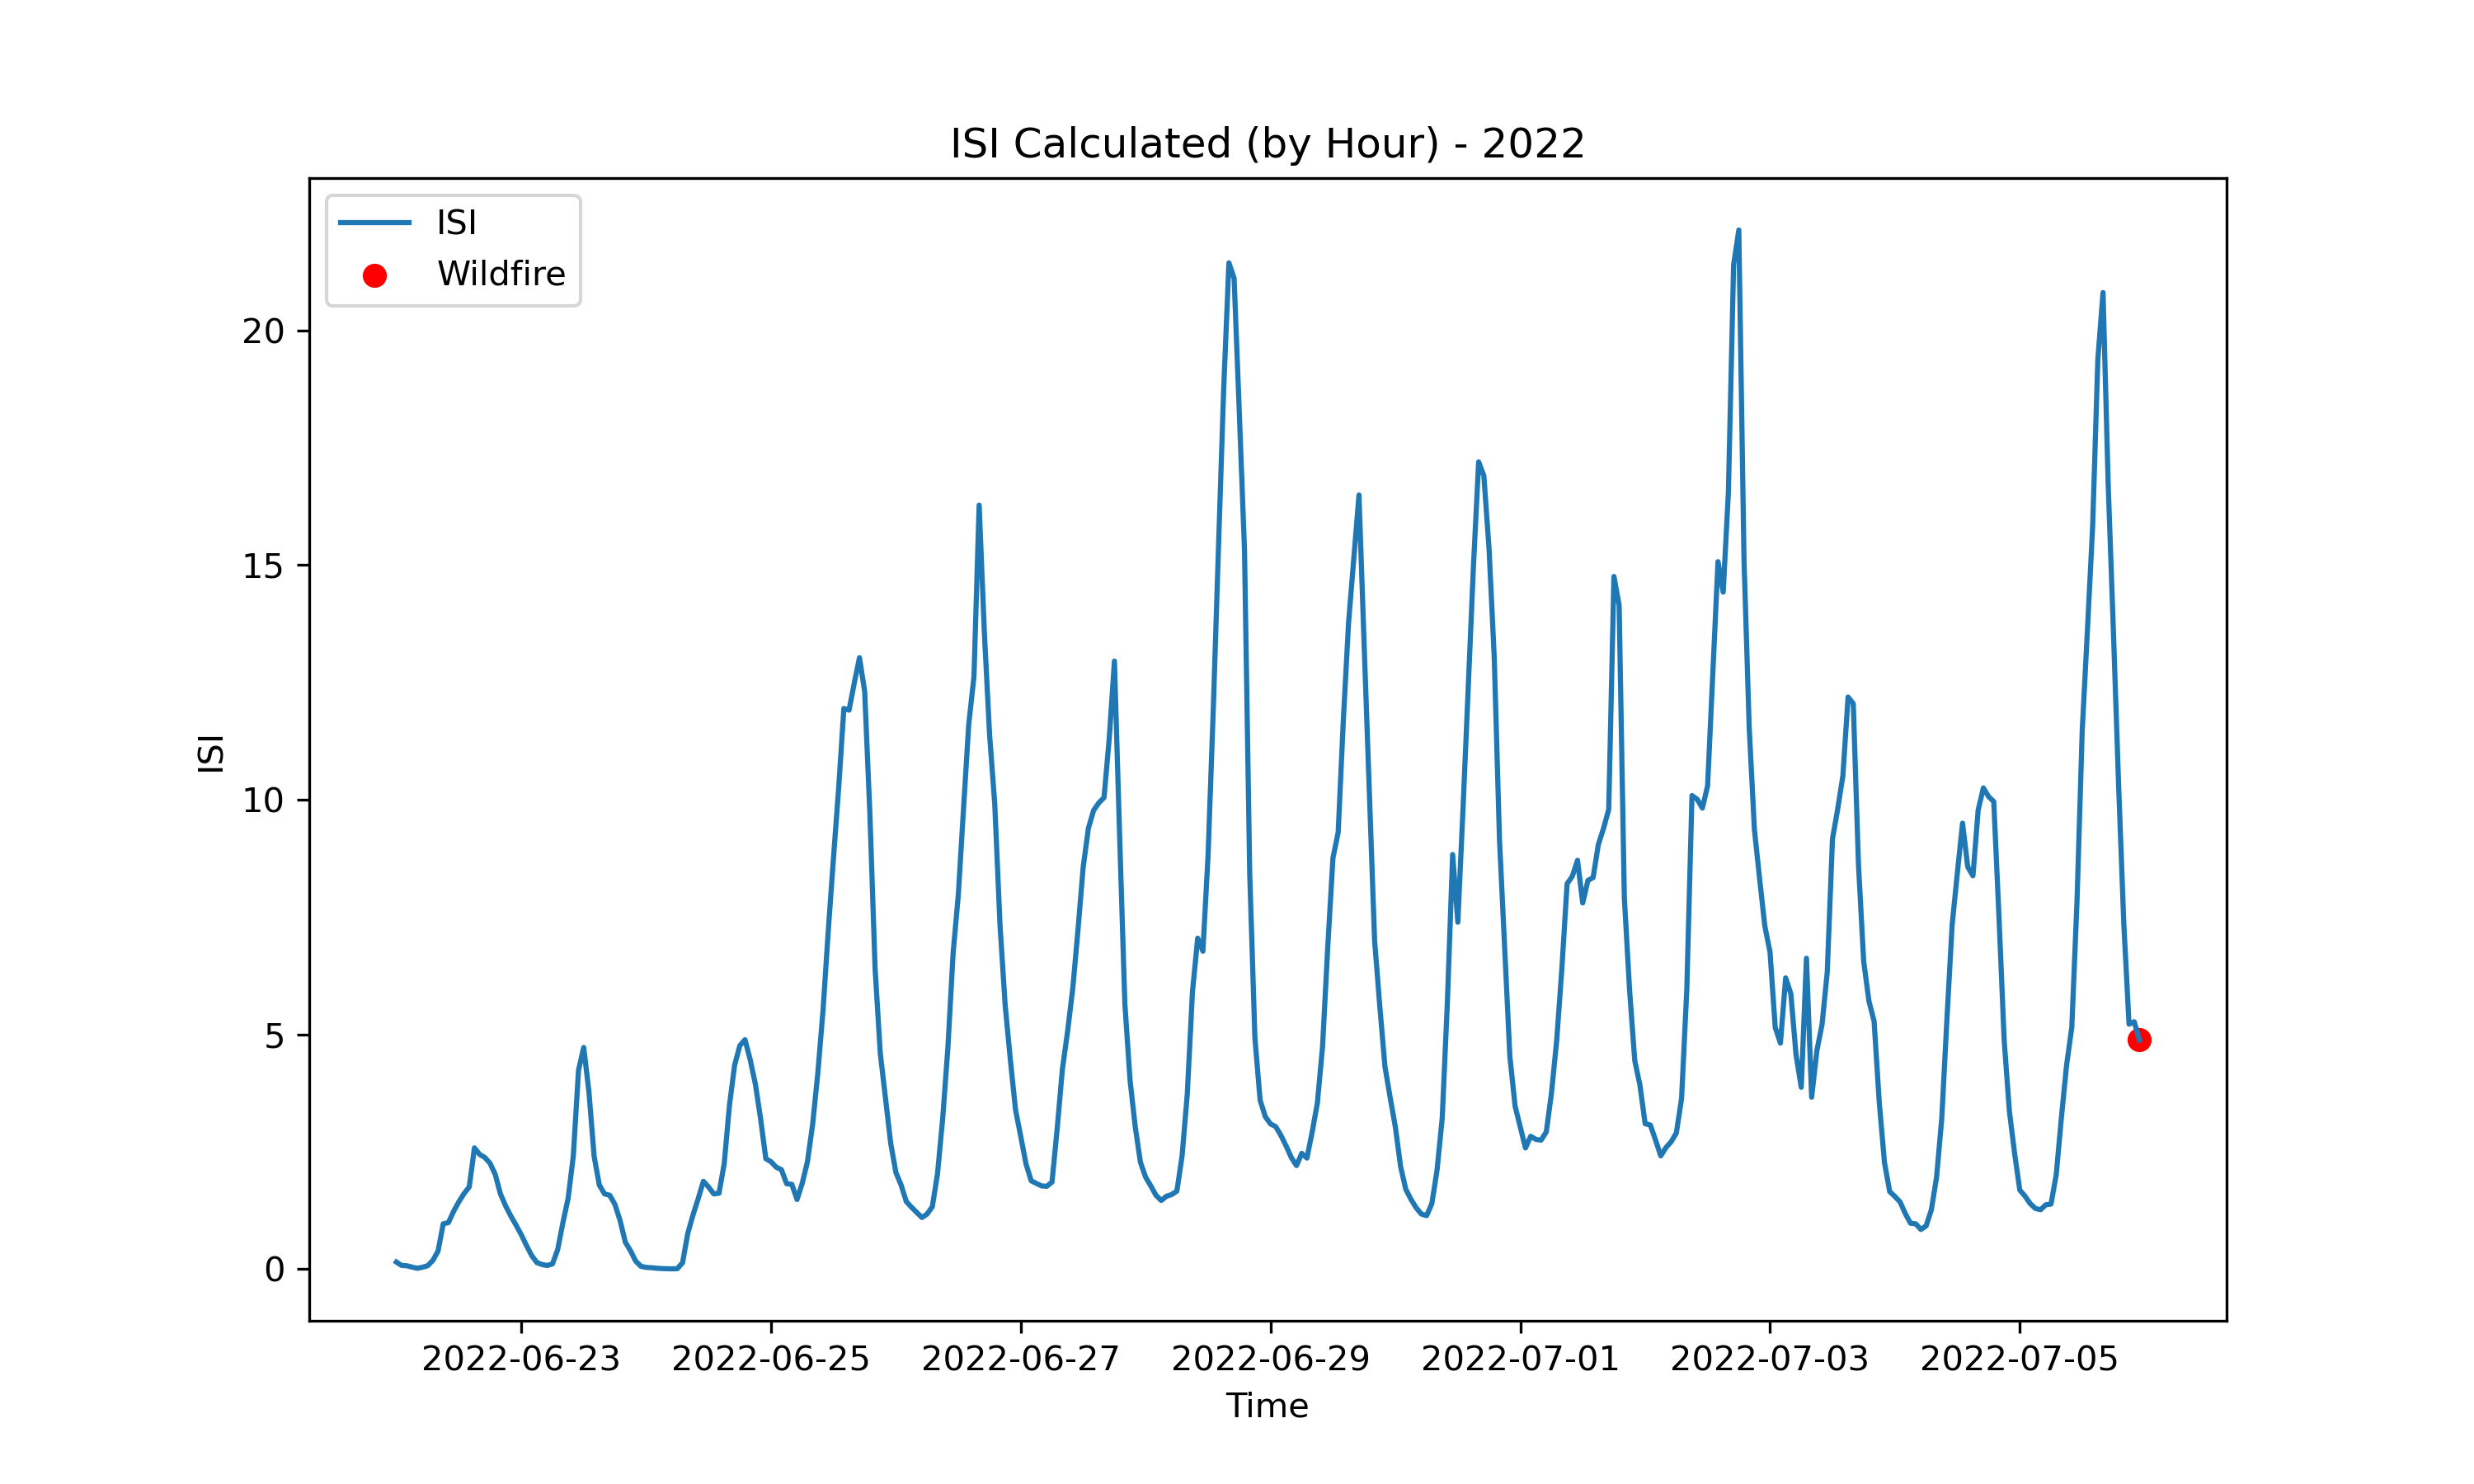
\includegraphics[width=\textwidth]{graphs/2022/2022CalcISI12.png}
	\end{subfigure}
	\label{fig:hourly_isi}
\end{figure}

\begin{figure}[h]
	\centering
	\caption{Calculated hourly BUI value for 2015, 2019, and 2022}
	\begin{subfigure}{0.45\textwidth}
		\centering
		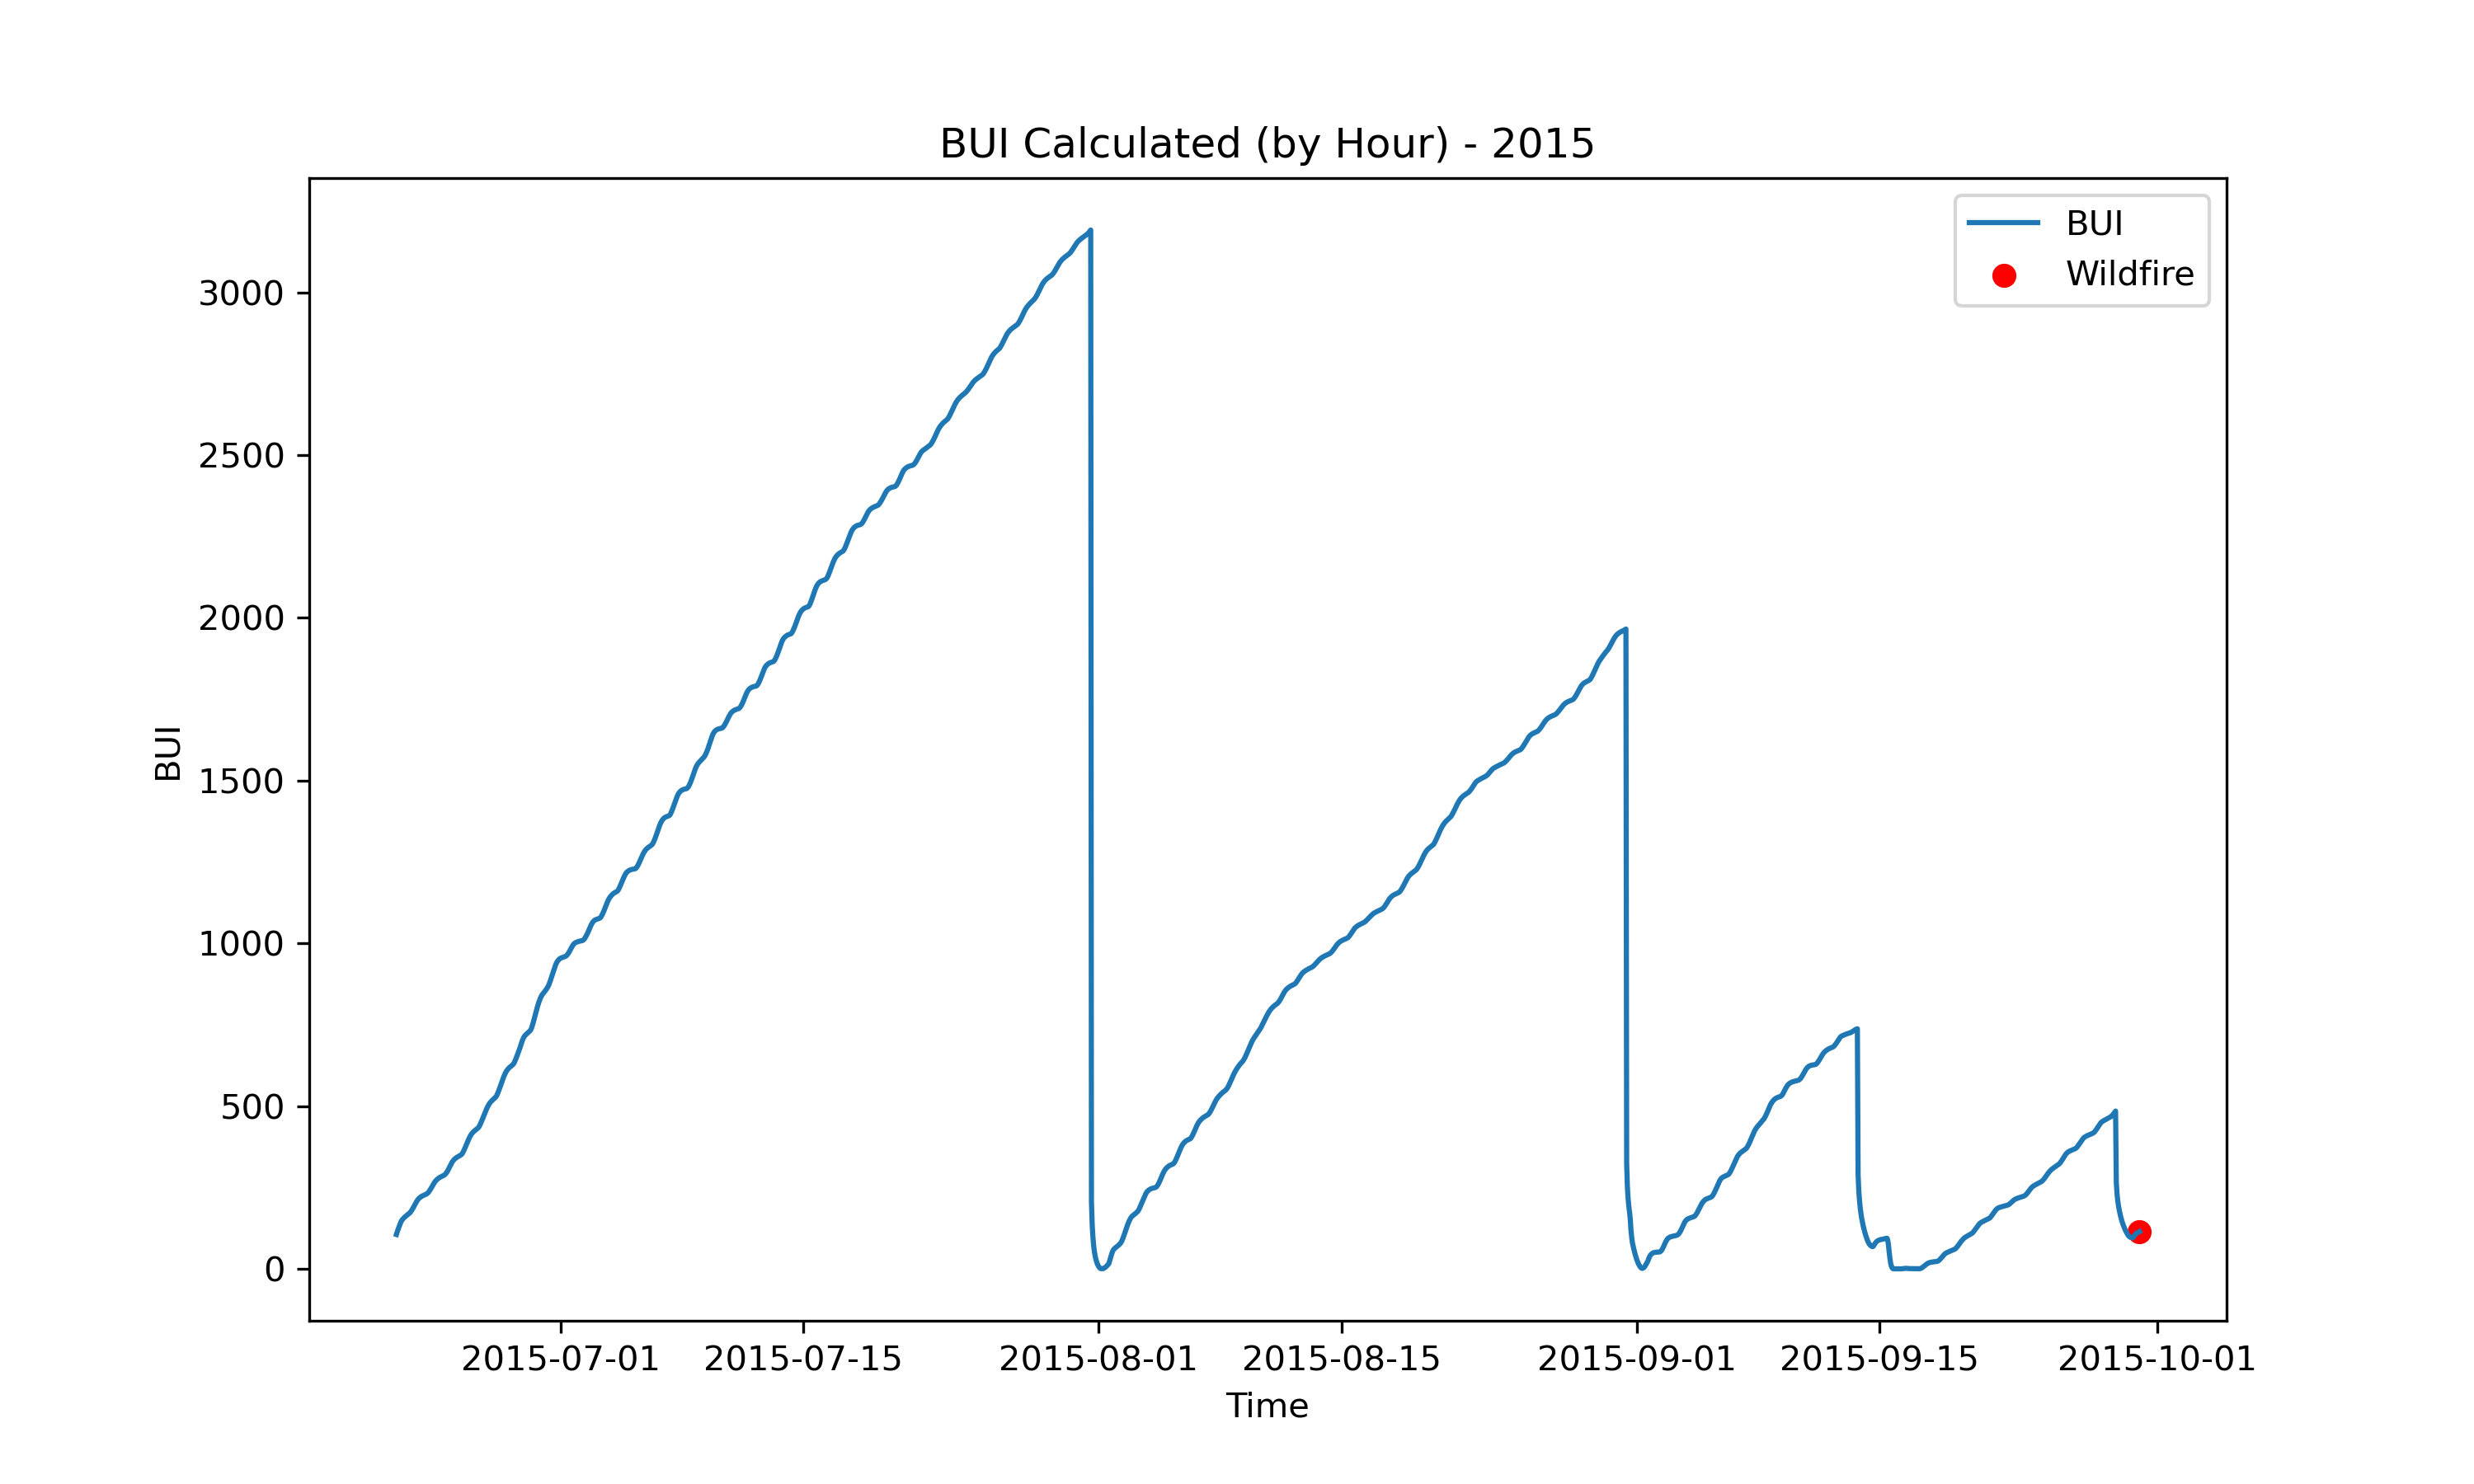
\includegraphics[width=\textwidth]{graphs/2015/byHour/2015CalcBUI12.png}
	\end{subfigure}
	\hfill
	\begin{subfigure}{0.45\textwidth}
		\centering
		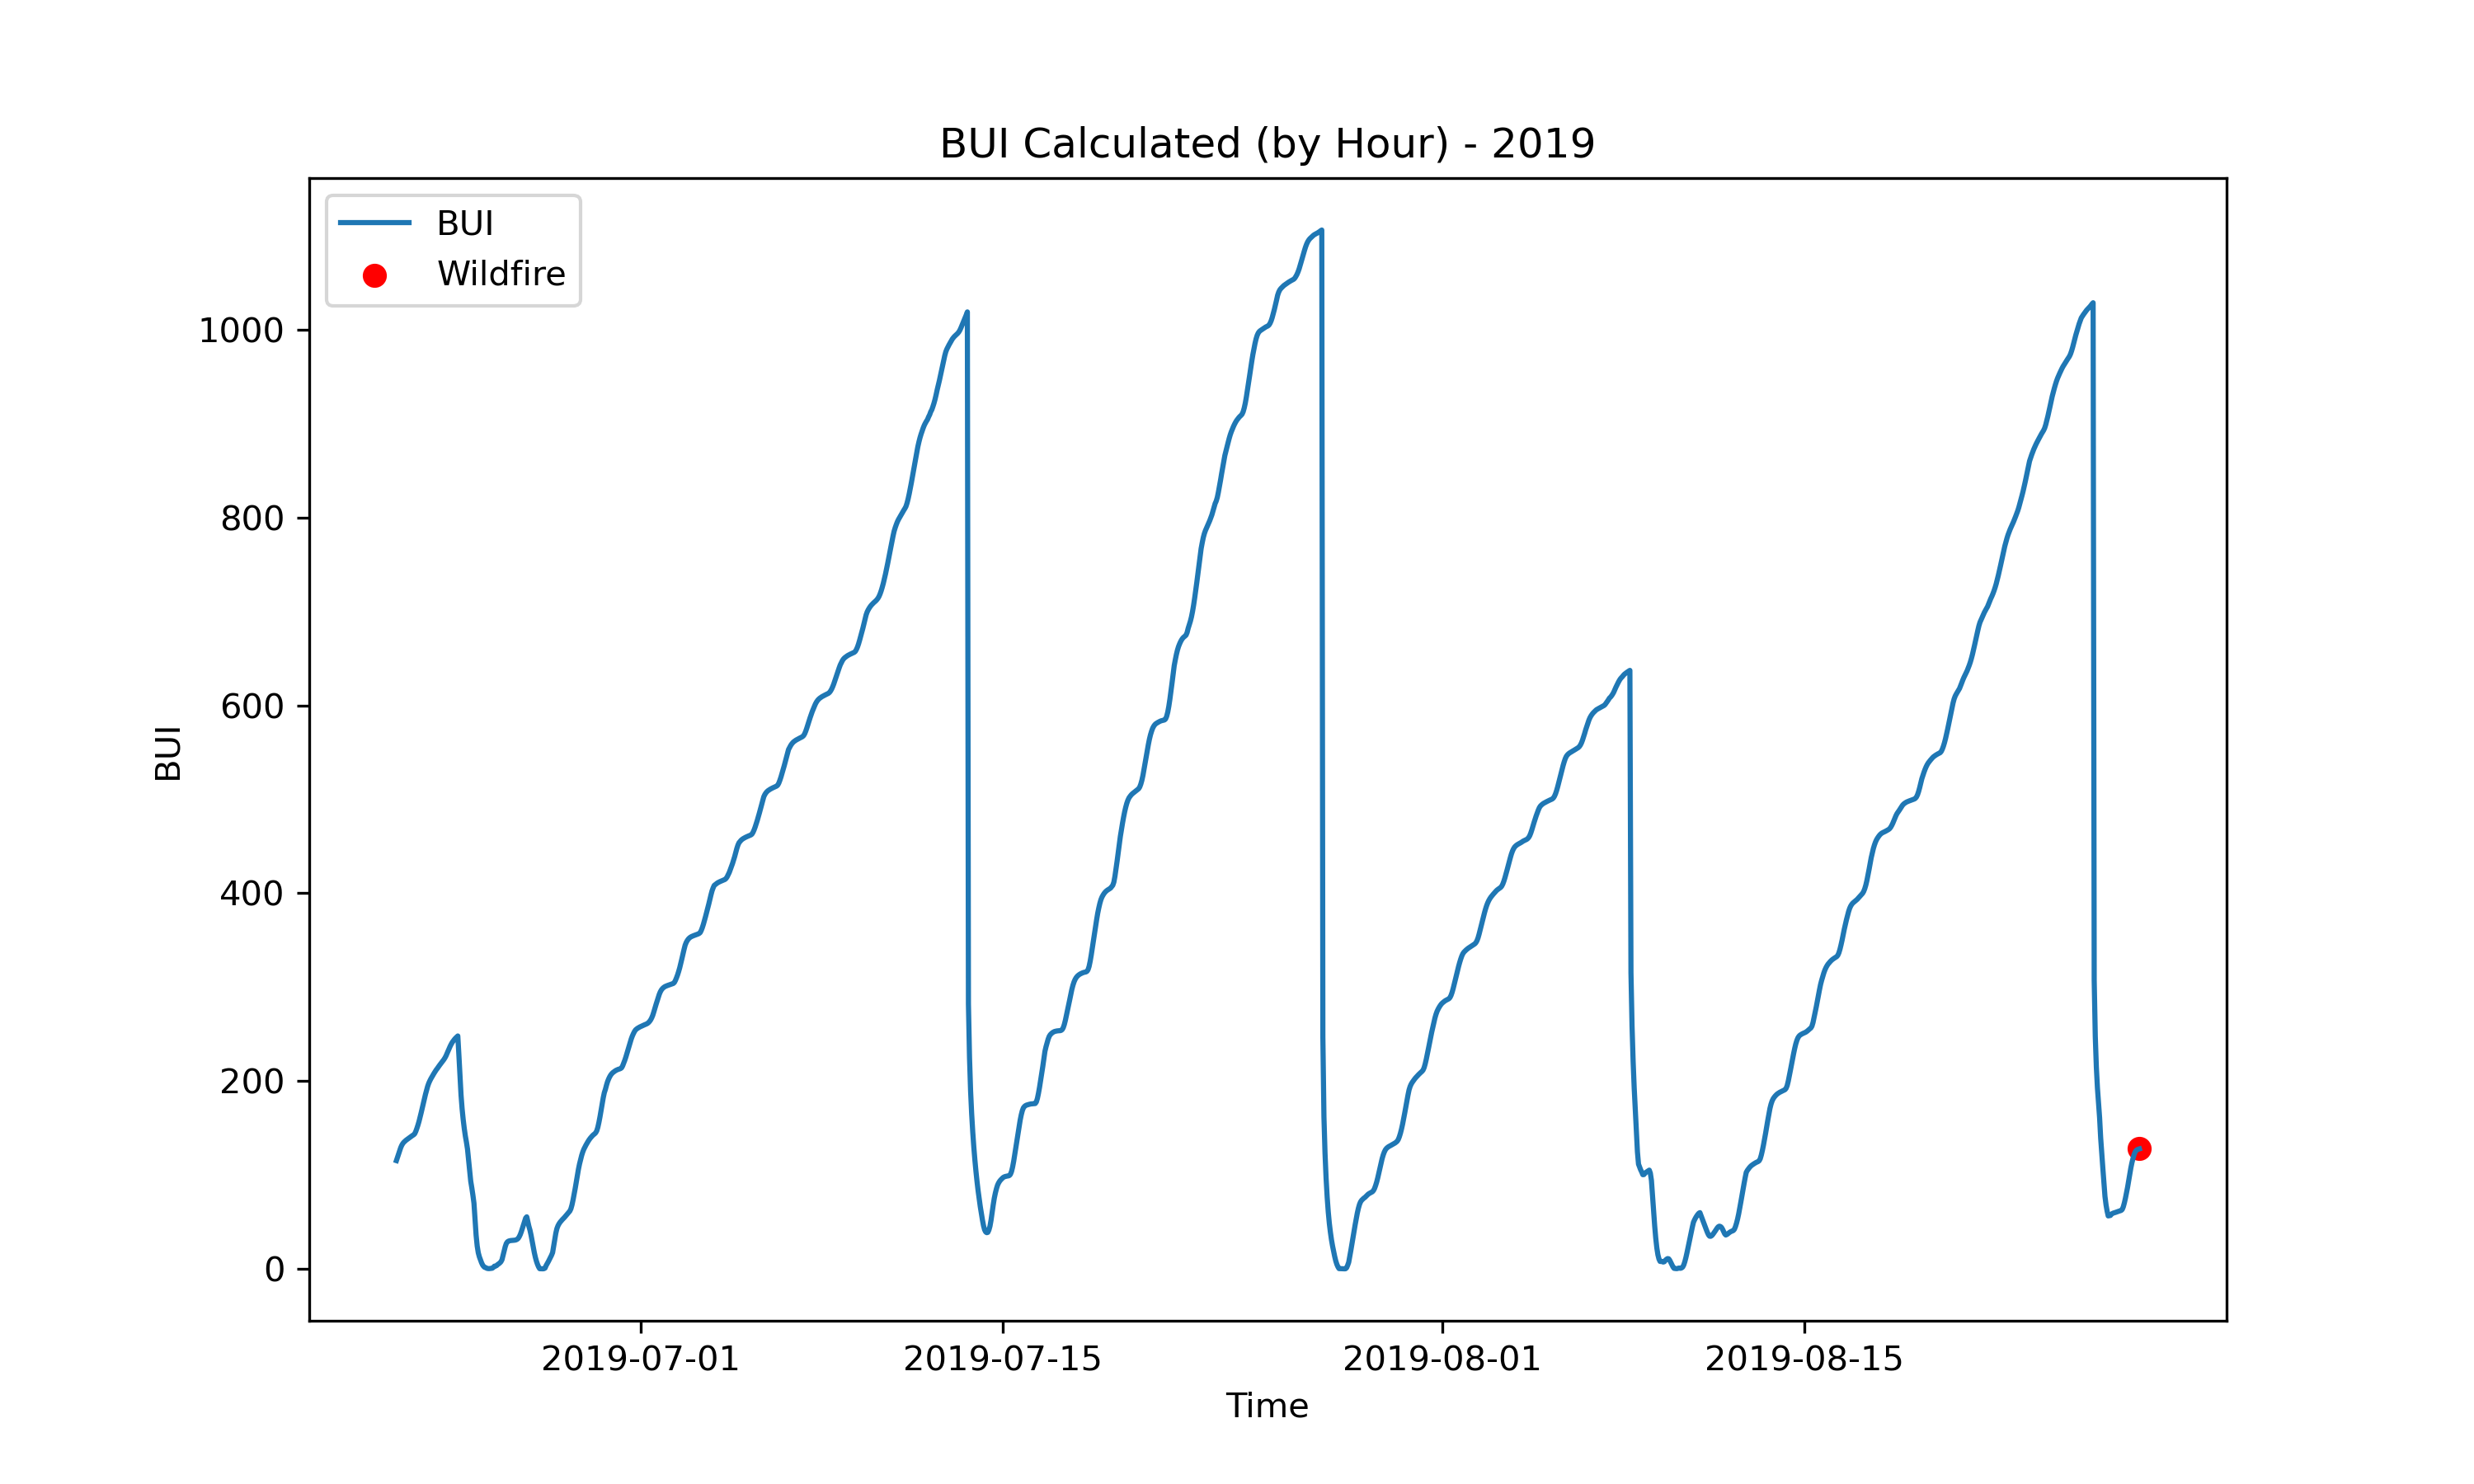
\includegraphics[width=\textwidth]{graphs/2019/2019CalcBUI12.png}
		\caption{Caption for image 2}
		\label{fig:img2}
	\end{subfigure}
	\hfill
	\begin{subfigure}{0.45\textwidth}
		\centering
		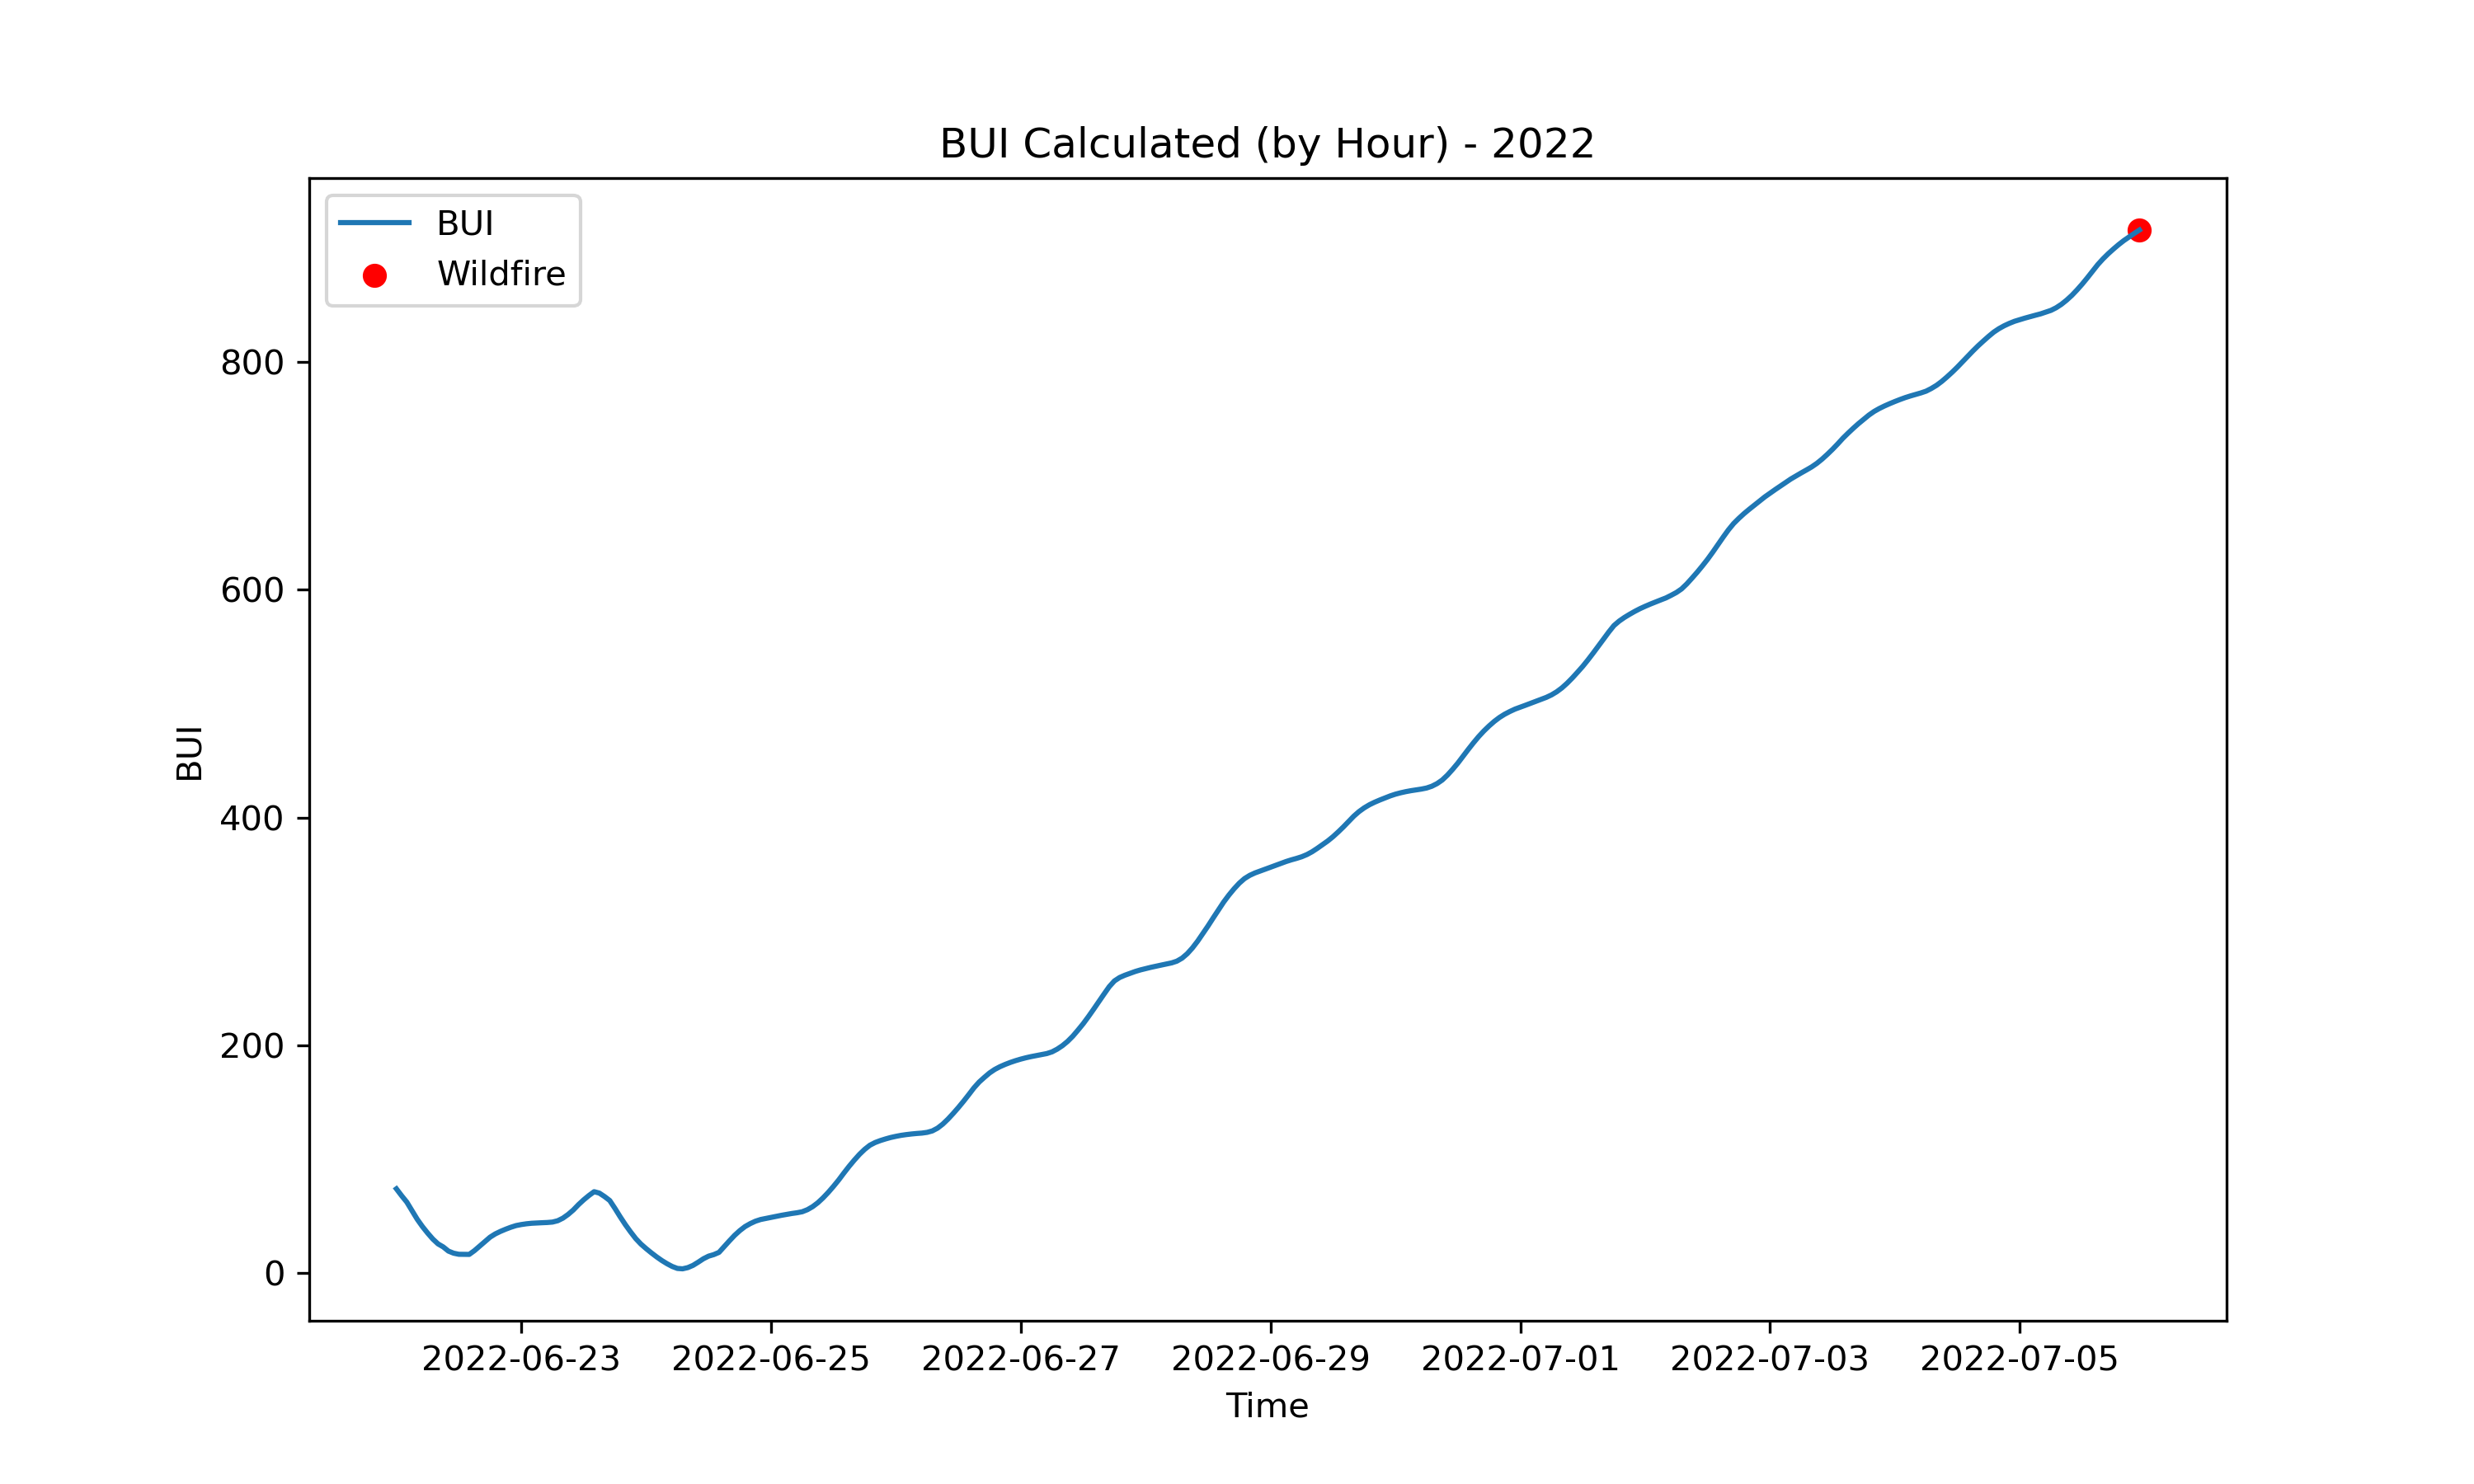
\includegraphics[width=\textwidth]{graphs/2022/2022CalcBUI12.png}
	\end{subfigure}
	
	\label{fig:hourly_bui}
\end{figure}

\FloatBarrier

\section{Evolution of maximum and minimum daily values of FWI variables}
\begin{figure}[h]
	\centering
	\caption{Daily max and min FWI values}
	\begin{subfigure}{0.45\textwidth}
		\centering
		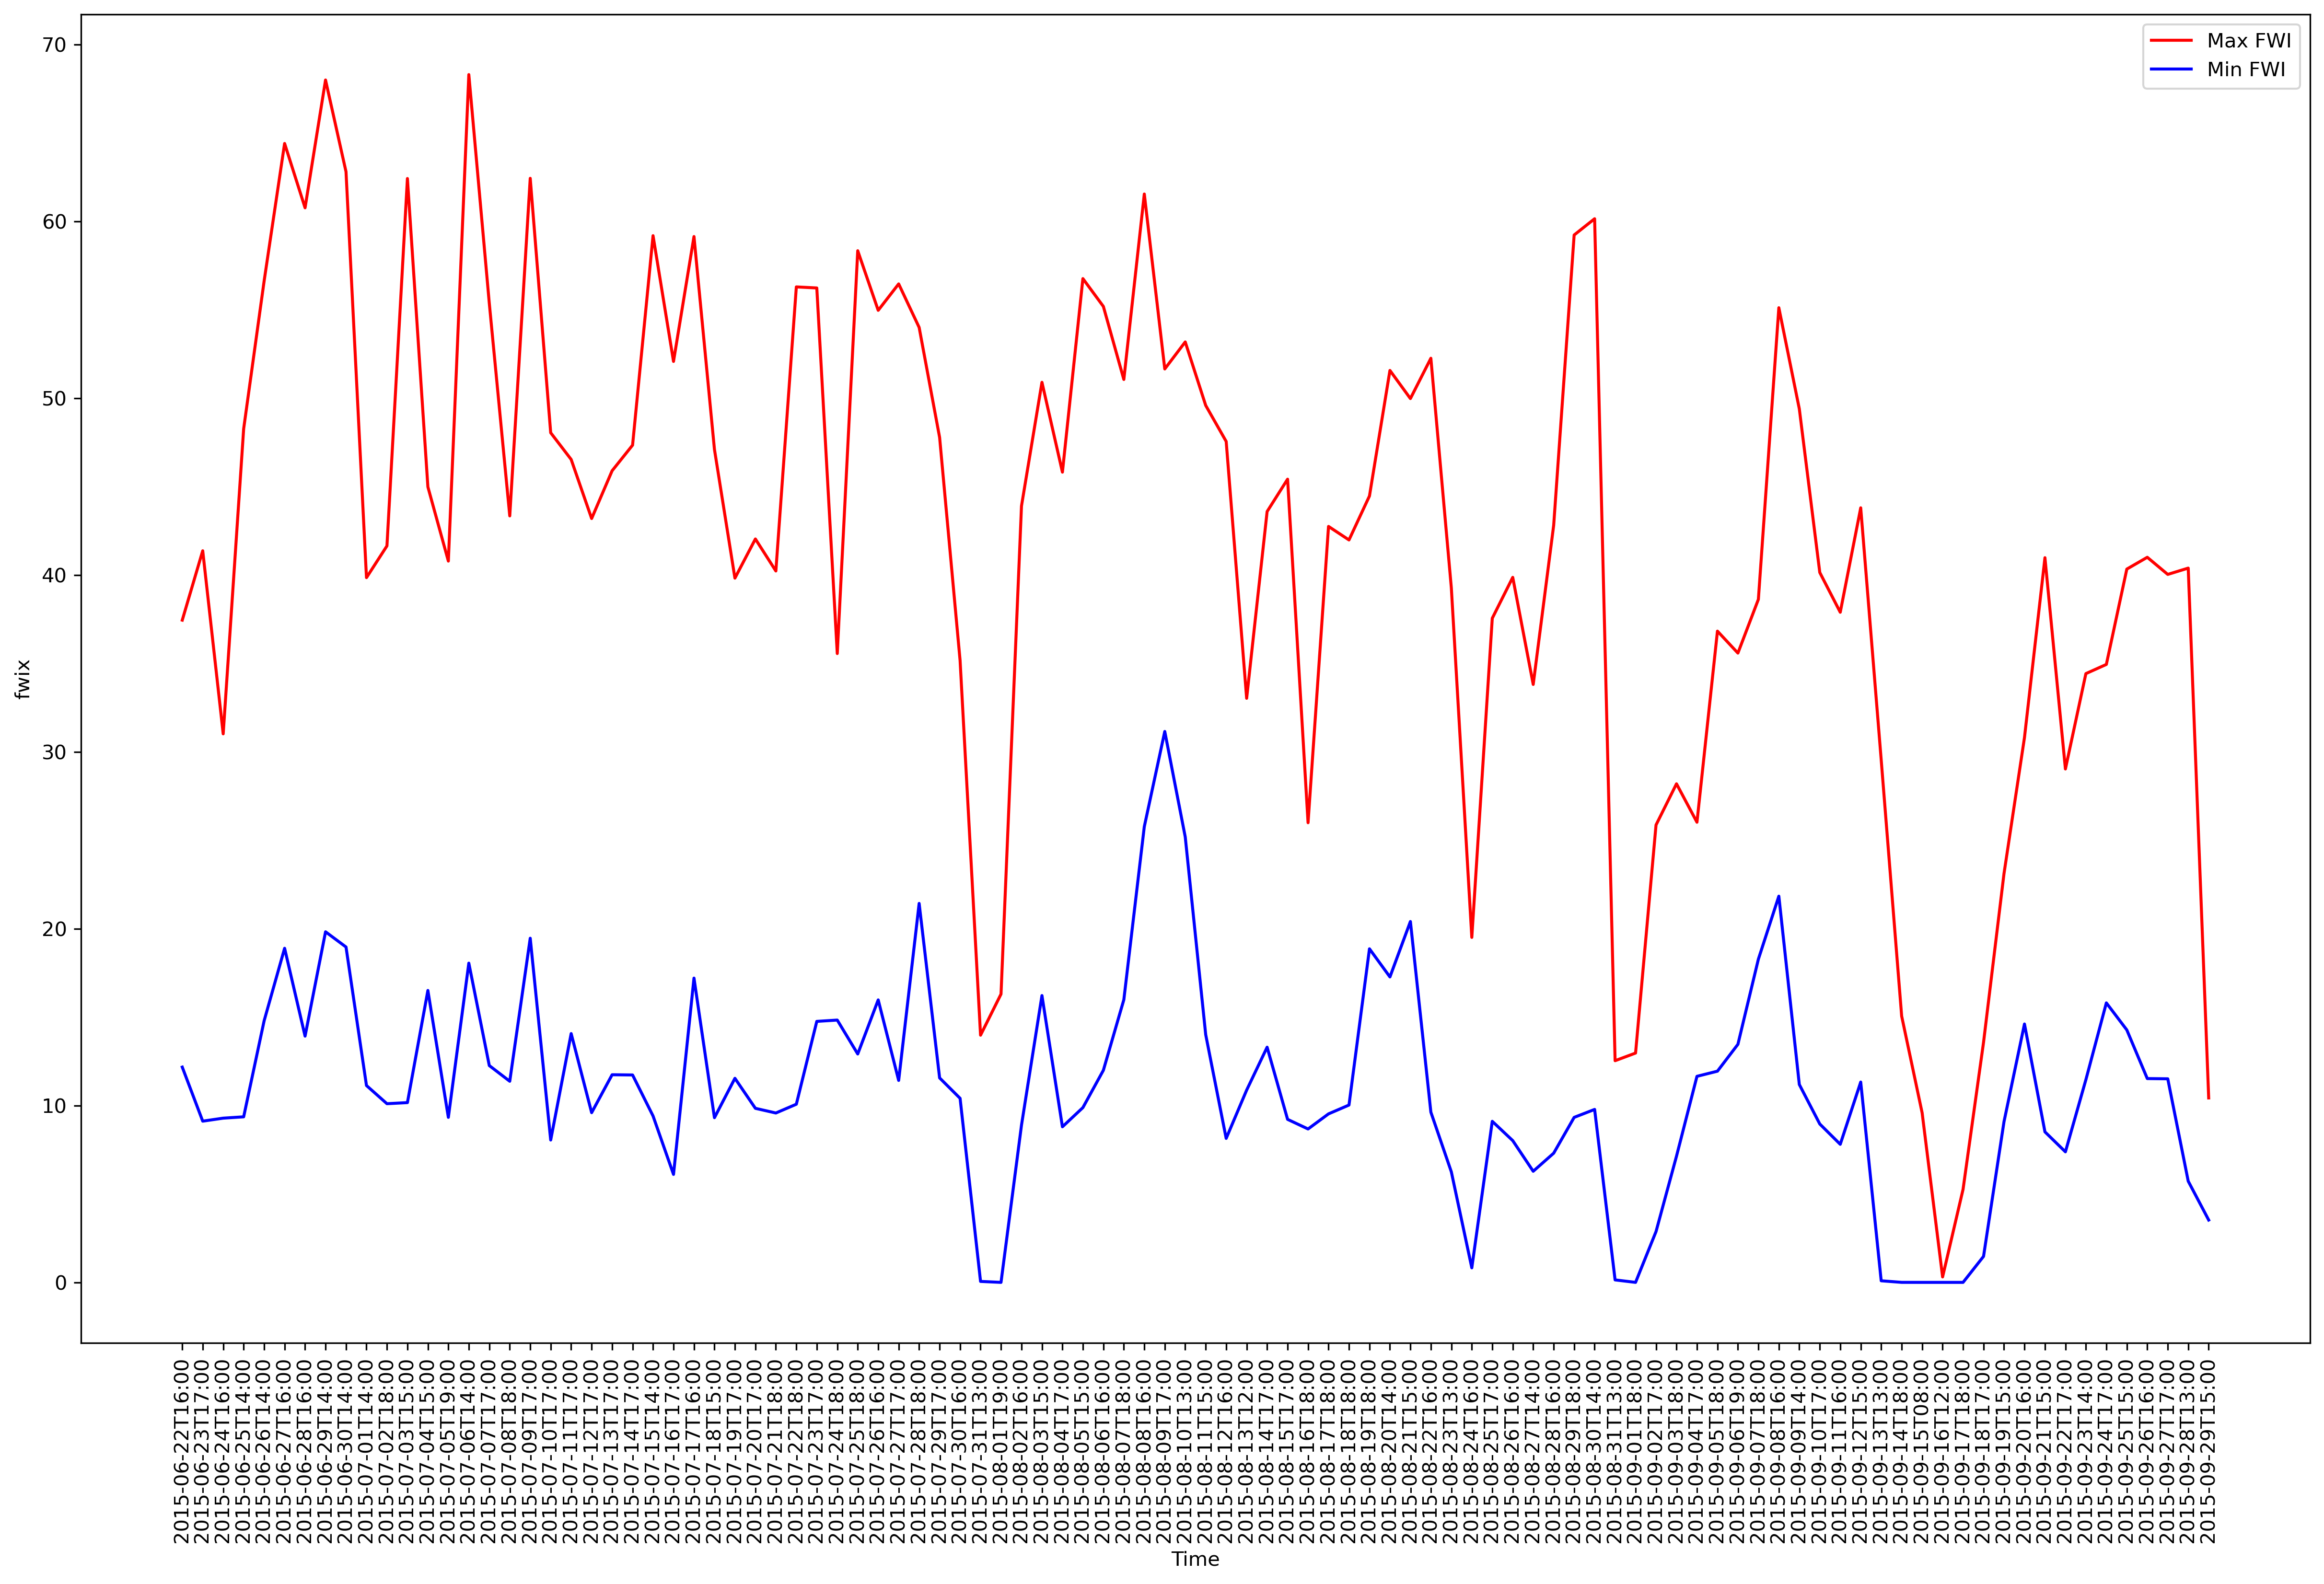
\includegraphics[width=\textwidth]{graphs/2015/byHour/FWI_maxMin.png}
		\caption{2015}
	\end{subfigure}
	\hfill
	\begin{subfigure}{0.45\textwidth}
		\centering
		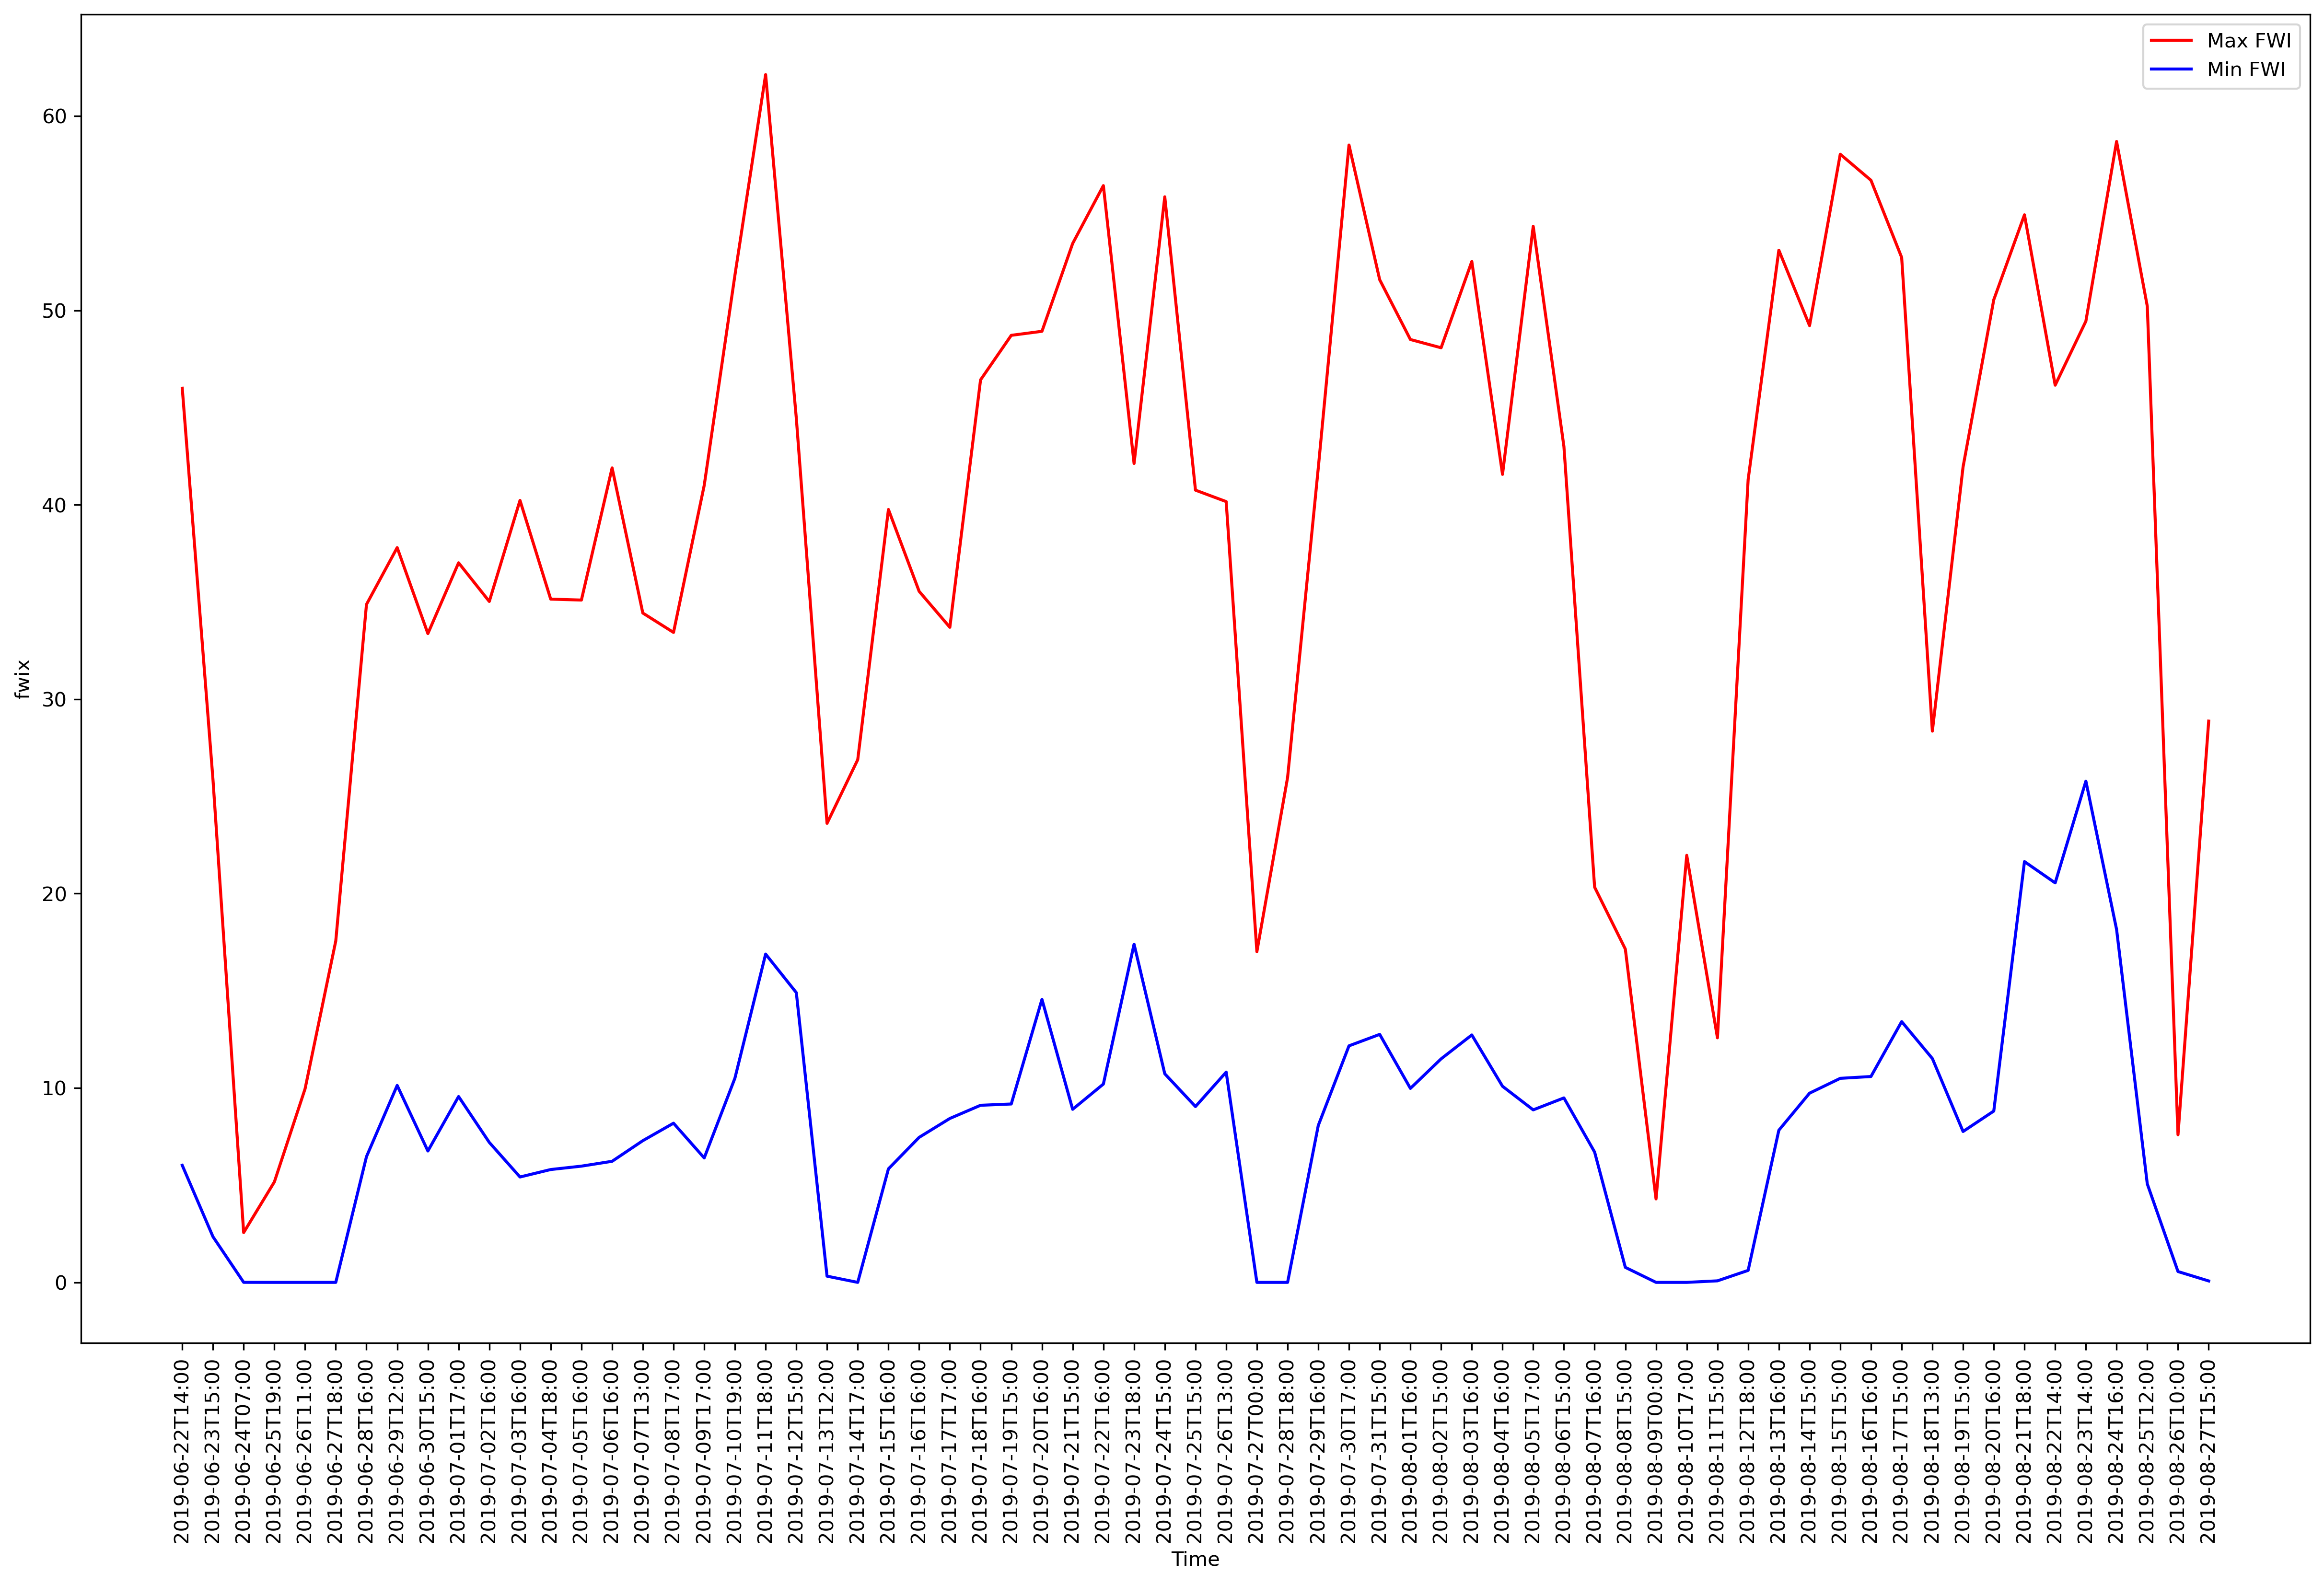
\includegraphics[width=\textwidth]{graphs/2019/byHour/FWI_maxMin.png}
		\caption{2019}
	\end{subfigure}
	\hfillFirstly, for each sample, a wildfire occurrence was set 3 hours before the wildfire occurrence and 1 hour after, then the most important variables were calculated. Their complete hourly record were used. With a random state of 445621151 for RandomForestClassifier, the tables \ref{importance_2015_2019} and \ref{importance_2022} shows the results for each year.
	\begin{subfigure}{0.45\textwidth}
		\centering
		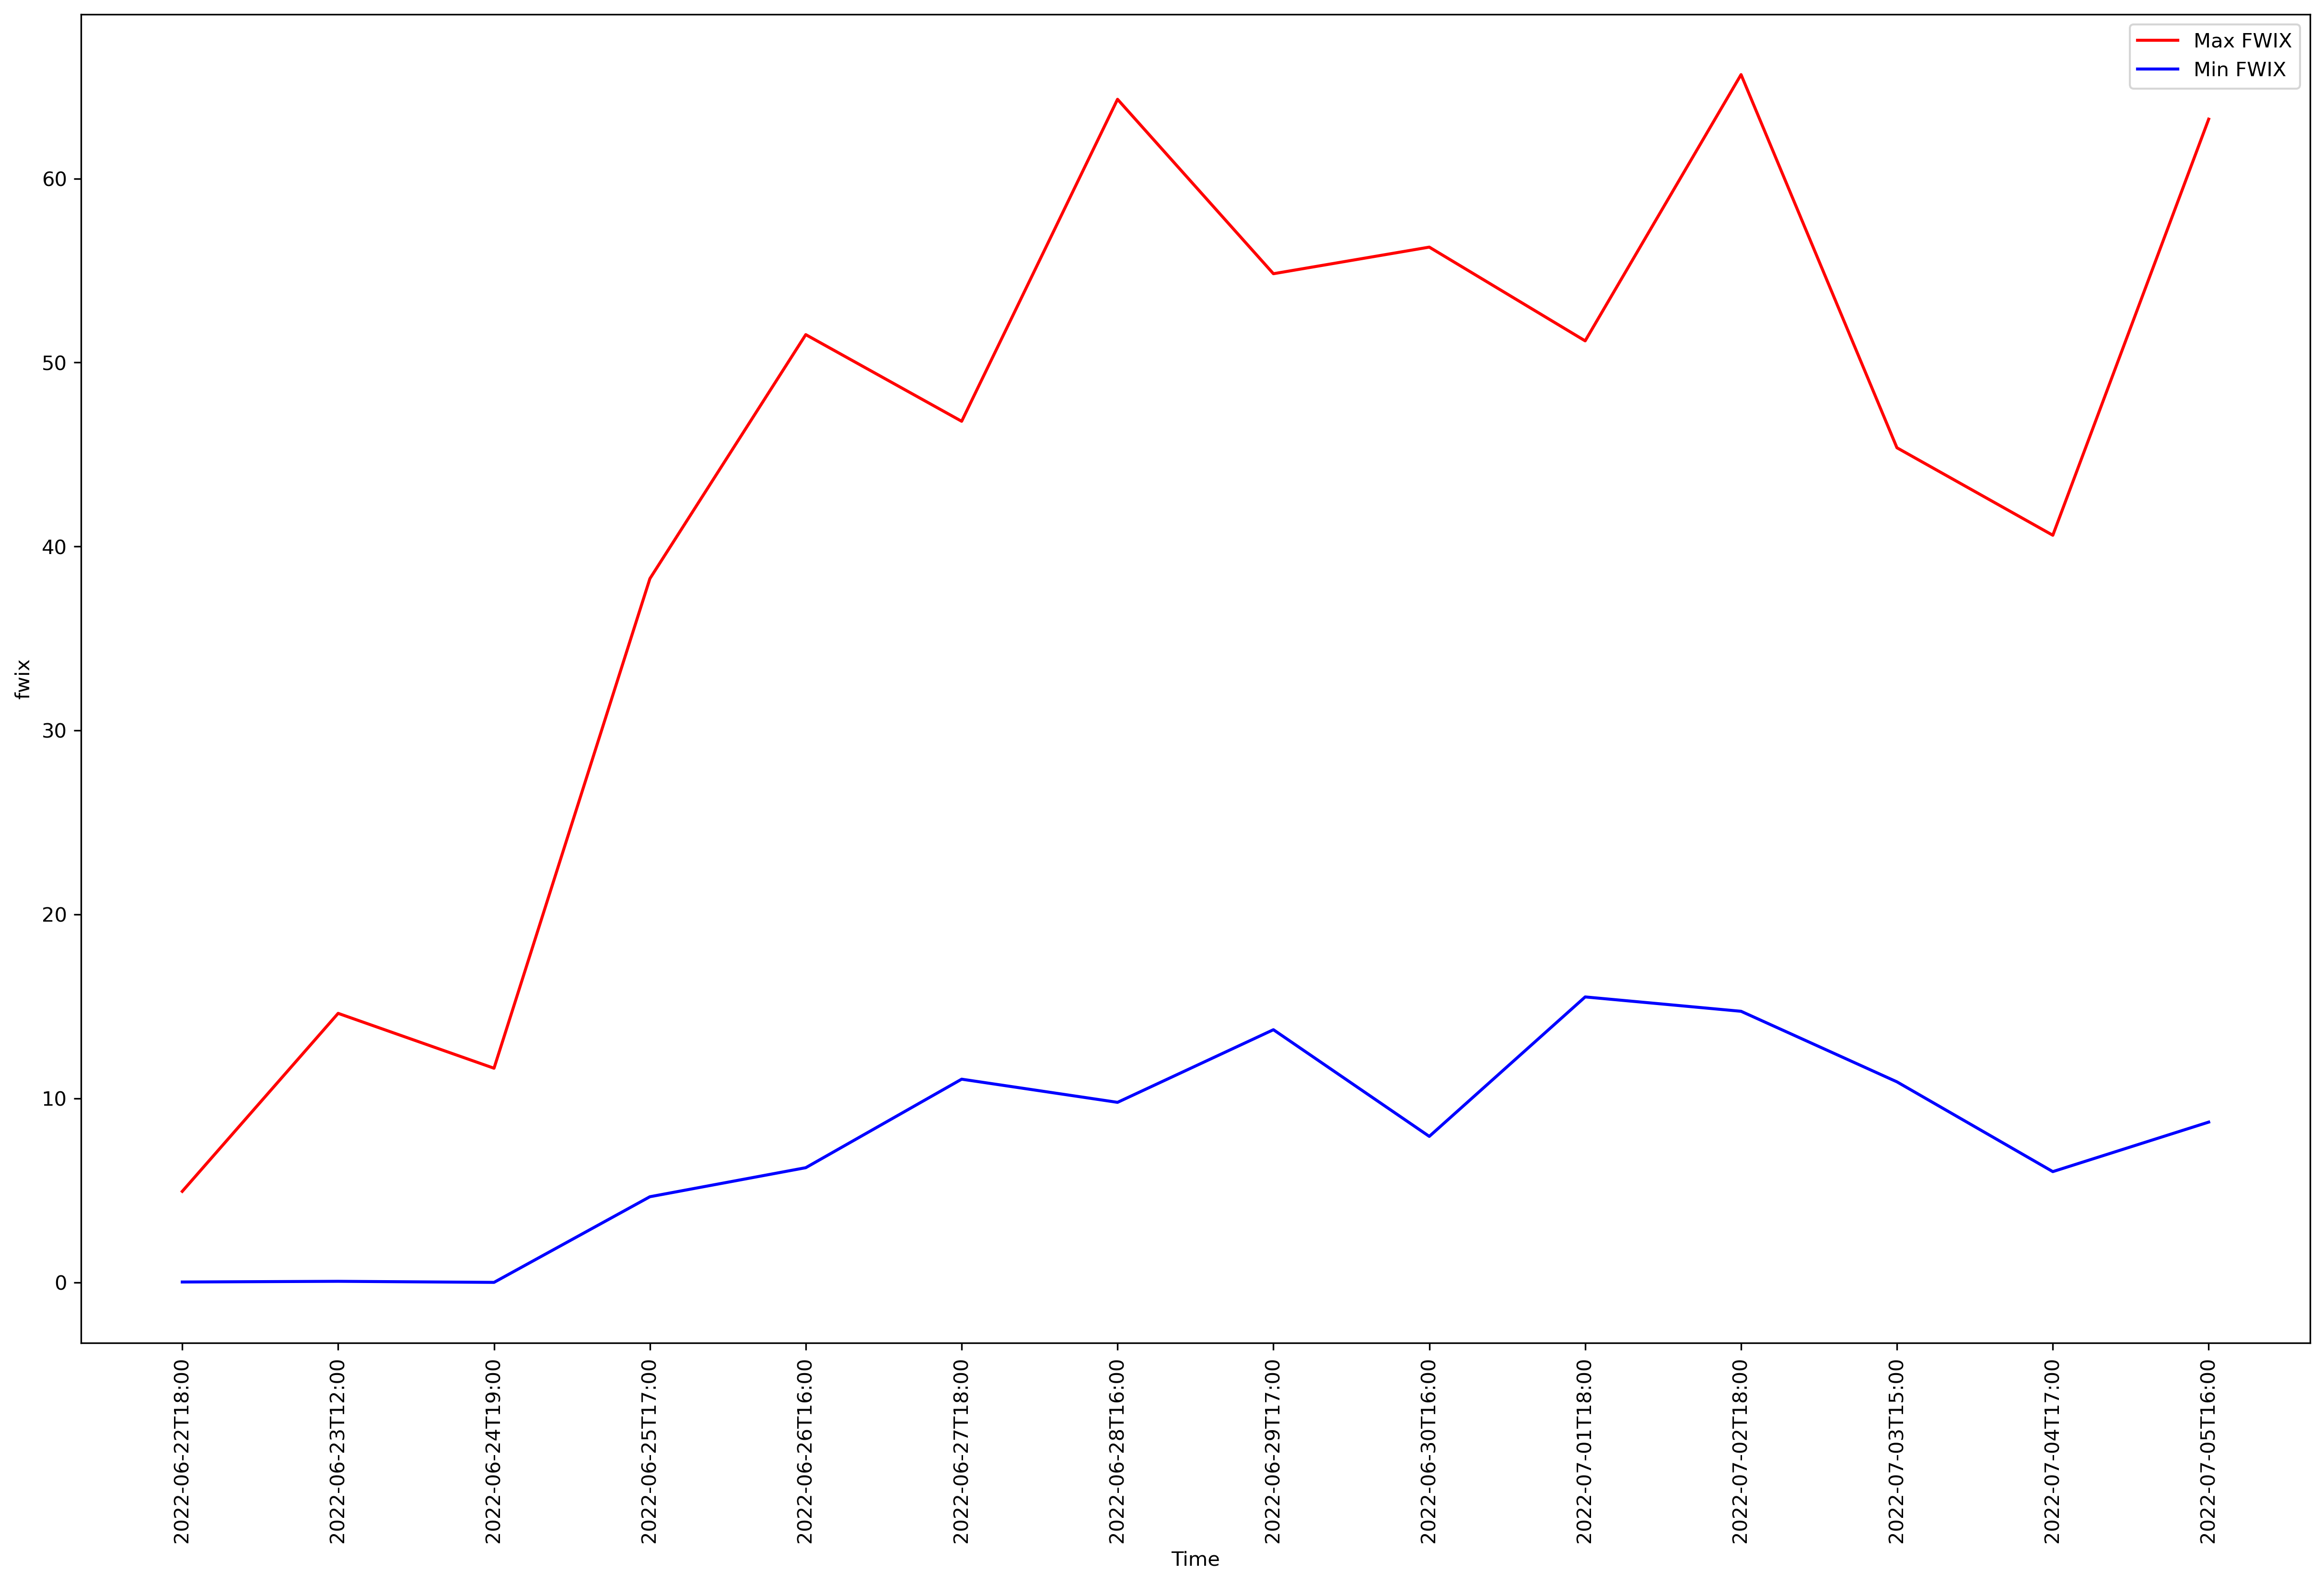
\includegraphics[width=\textwidth]{graphs/2022/FWIX_maxMin.png}
		\caption{2022}
	\end{subfigure}
	
	\label{fig:daily_fwix_maxmin}
\end{figure}

\begin{figure}[h]
	\centering
	\caption{Daily max and min FFMC values}
	\begin{subfigure}{0.45\textwidth}
		\centering
		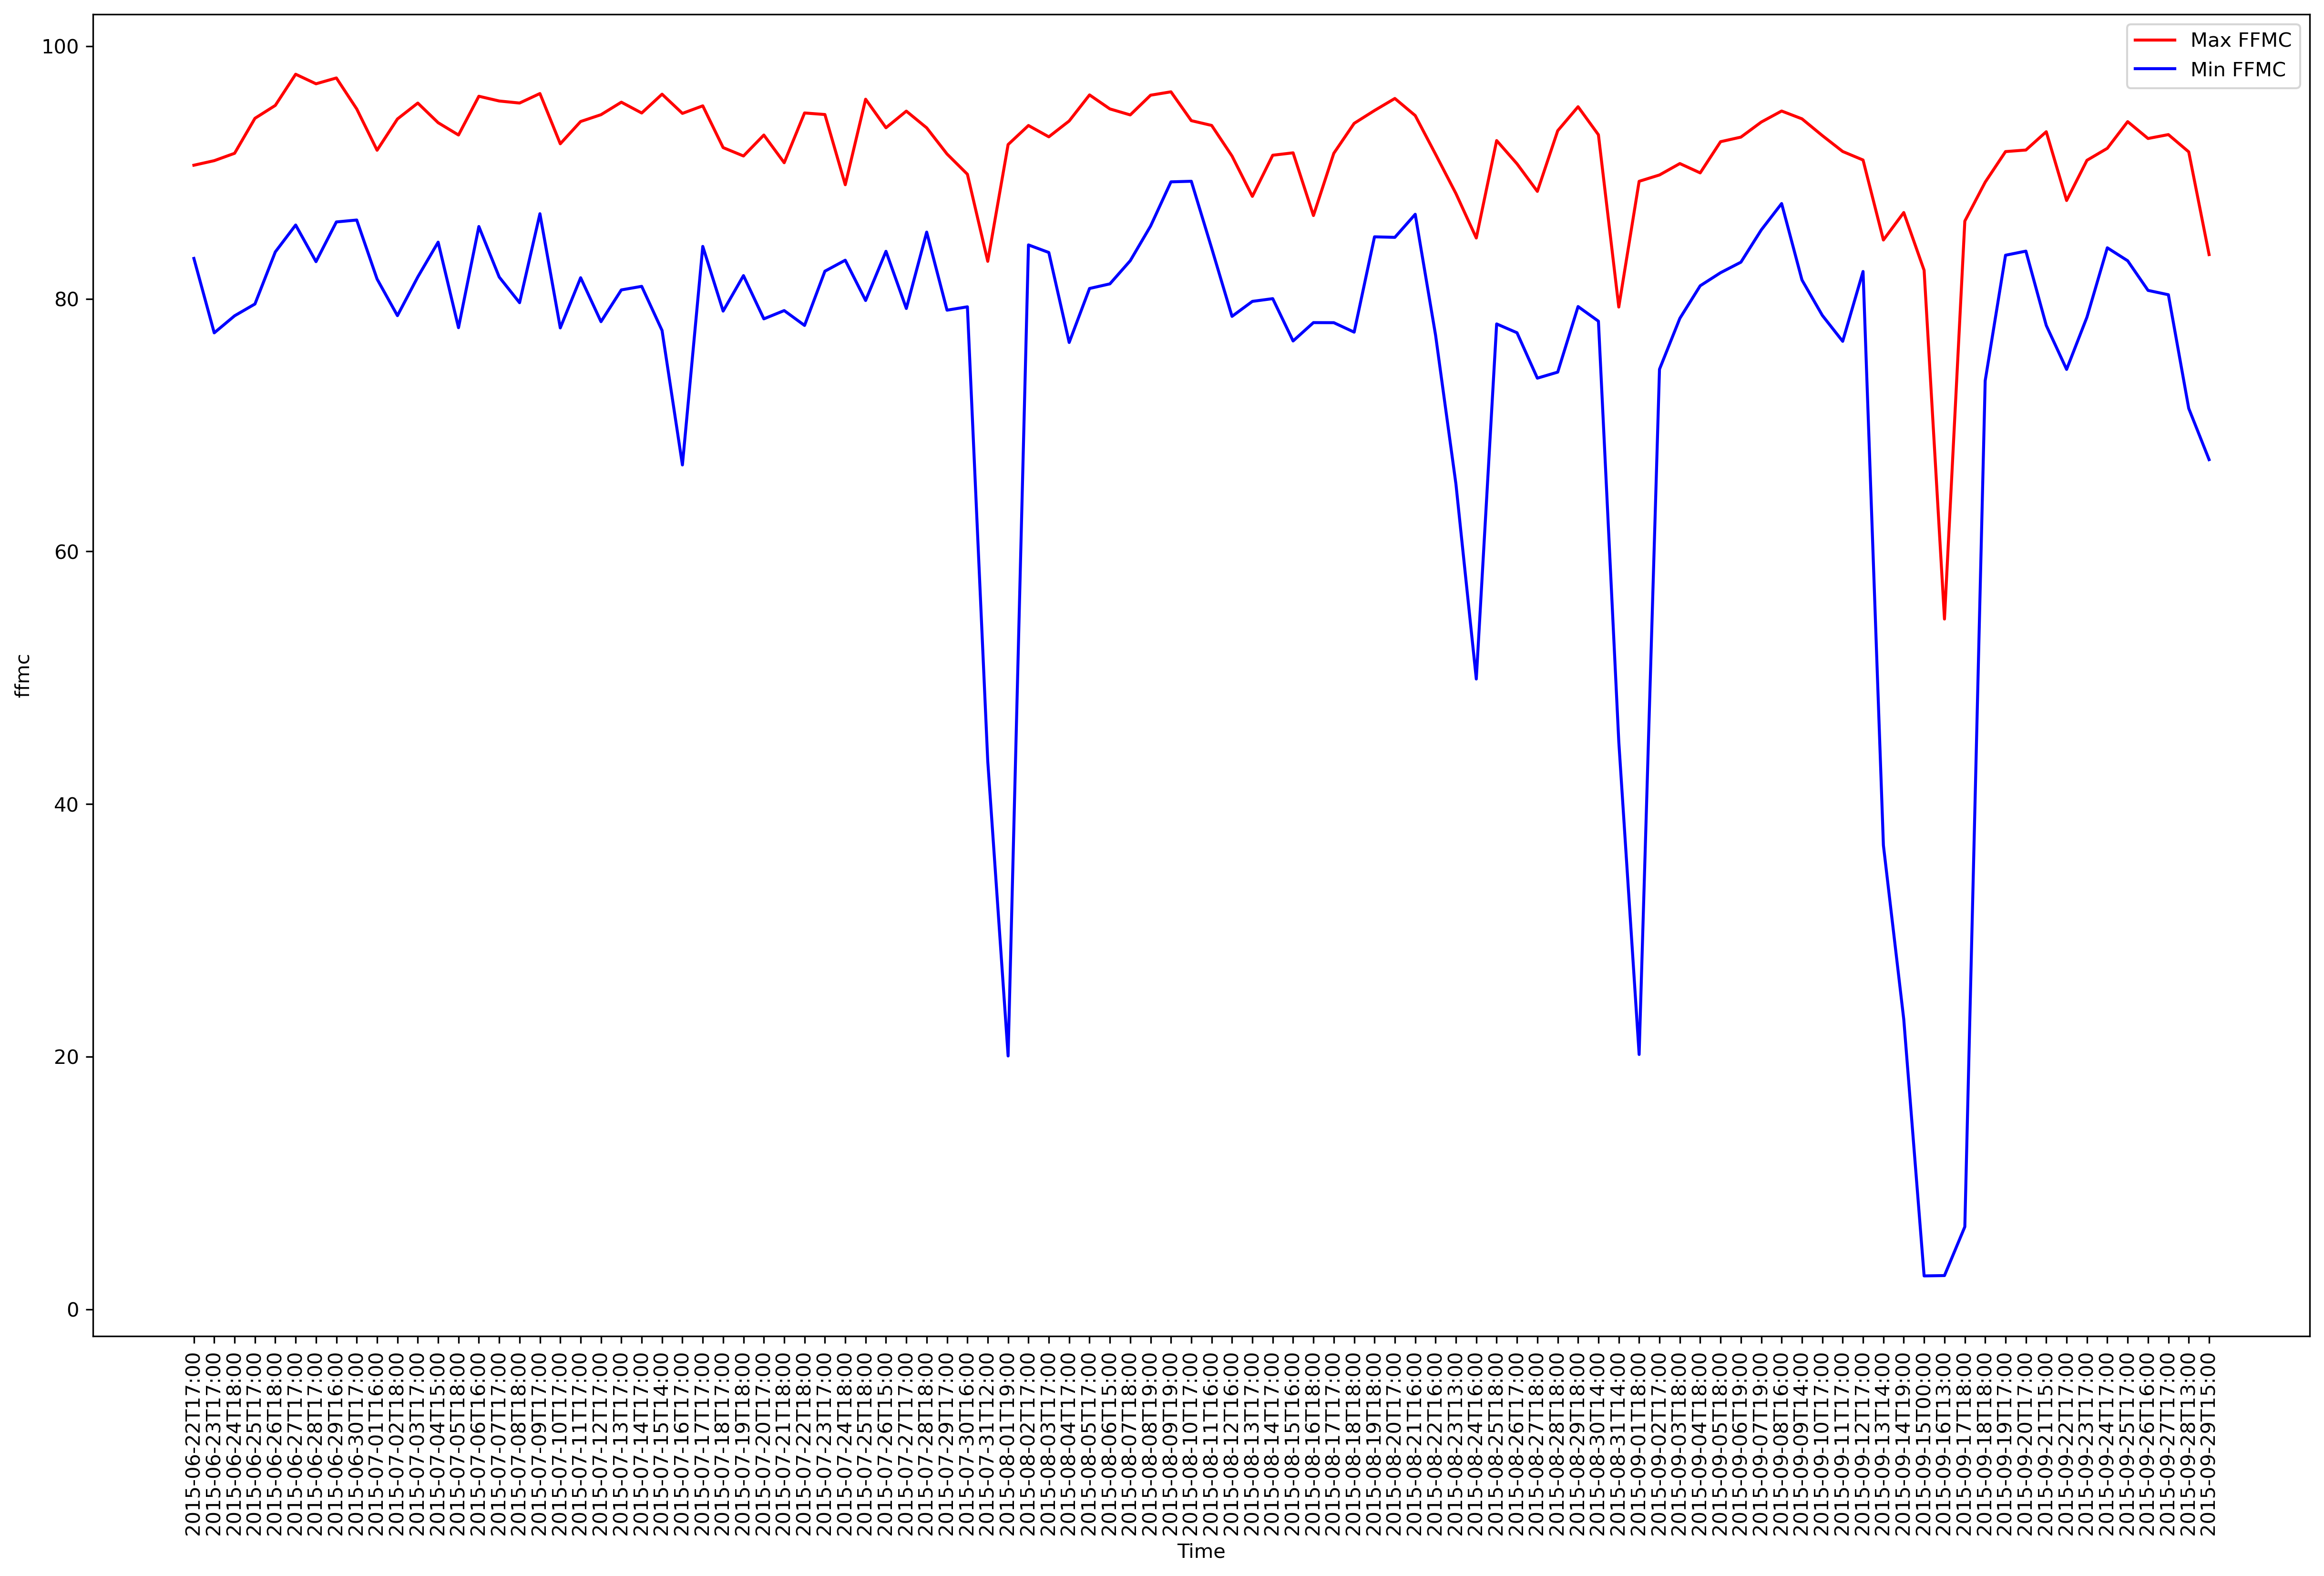
\includegraphics[width=\textwidth]{graphs/2015/byHour/FFMC_maxMin.png}
		\caption{2015}
	\end{subfigure}
	\hfill
	\begin{subfigure}{0.45\textwidth}
		\centering
		\includegraphics[width=\textwidth]{graphs/2019/byHour/FFMC_maxMin.png}
		\caption{2019}
	\end{subfigure}
	\hfill
	\begin{subfigure}{0.45\textwidth}
		\centering
		\includegraphics[width=\textwidth]{graphs/2022/FFMC_maxMin.png}
		\caption{2022}
	\end{subfigure}
	
	\label{fig:daily_ffmc_maxmin}
\end{figure}


\begin{figure}[h]
	\centering
	\caption{Daily max and min DMC values}
	\begin{subfigure}{0.45\textwidth}
		\centering
		\includegraphics[width=\textwidth]{graphs/2015/byHour/DMC_maxMin.png}
		\caption{2015}
	\end{subfigure}
	\hfill
	\begin{subfigure}{0.45\textwidth}
		\centering
		\includegraphics[width=\textwidth]{graphs/2019/byHour/DMC_maxMin.png}
		\caption{2019}
	\end{subfigure}
	\hfill
	\begin{subfigure}{0.45\textwidth}
		\centering
		\includegraphics[width=\textwidth]{graphs/2022/DMC_maxMin.png}
		\caption{2022}
	\end{subfigure}
	
	\label{fig:daily_dmc_maxmin}
\end{figure}

\begin{figure}[h]
	\centering
	\caption{Daily max and min DC values}
	\begin{subfigure}{0.45\textwidth}
		\centering
		\includegraphics[width=\textwidth]{graphs/2015/byHour/DC_maxMin.png}
		\caption{2015}
	\end{subfigure}
	\hfill
	\begin{subfigure}{0.45\textwidth}
		\centering
		\includegraphics[width=\textwidth]{graphs/2019/byHour/DC_maxMin.png}
		\caption{2019}
	\end{subfigure}
	\hfill
	\begin{subfigure}{0.45\textwidth}
		\centering
		\includegraphics[width=\textwidth]{graphs/2022/DC_maxMin.png}
		\caption{2022}
	\end{subfigure}
	
	\label{fig:daily_dc_maxmin}
\end{figure}

\begin{figure}[h]
	\centering
	\caption{Daily max and min ISI values}
	\begin{subfigure}{0.45\textwidth}
		\centering
		\includegraphics[width=\textwidth]{graphs/2015/byHour/ISI_maxMin.png}
		\caption{2015}
	\end{subfigure}
	\hfill
	\begin{subfigure}{0.45\textwidth}
		\centering
		\includegraphics[width=\textwidth]{graphs/2019/byHour/ISI_maxMin.png}
		\caption{2019}
	\end{subfigure}
	\hfill
	\begin{subfigure}{0.45\textwidth}
		\centering
		\includegraphics[width=\textwidth]{graphs/2022/ISI_maxMin.png}
		\caption{2022}
	\end{subfigure}
	\label{fig:daily_isi_maxmin}
\end{figure}

\begin{figure}[h]
	\centering
	\caption{Daily max and min BUI values}
	\begin{subfigure}{0.45\textwidth}
		\centering
		\includegraphics[width=\textwidth]{graphs/2015/byHour/BUI_maxMin.png}
		\caption{2015}
	\end{subfigure}
	\hfill
	\begin{subfigure}{0.45\textwidth}
		\centering
		\includegraphics[width=\textwidth]{graphs/2019/byHour/BUI_maxMin.png}
		\caption{2019}
	\end{subfigure}
	\hfill
	\begin{subfigure}{0.45\textwidth}
		\centering
		\includegraphics[width=\textwidth]{graphs/2022/BUI_maxMin.png}
		\caption{2022}
	\end{subfigure}
	\label{fig:daily_bui_maxmin}
\end{figure}

\FloatBarrier

\section{Before, after and daily maximum value}

\begin{figure}[h]
	\centering
	\caption{Before, after and daily FWI maximum value}
	\begin{subfigure}{0.45\textwidth}
		\centering
		\includegraphics[width=\textwidth]{graphs/2015/byHour/fwi_max_before_after.png}
		\caption{2015}
	\end{subfigure}
	\hfill
	\begin{subfigure}{0.45\textwidth}
		\centering
		\includegraphics[width=\textwidth]{graphs/2019/byHour/FWI_max_before_after.png}
		\caption{2019}
	\end{subfigure}
	\hfill
	\begin{subfigure}{0.45\textwidth}
		\centering
		\includegraphics[width=\textwidth]{graphs/2022/FWI_max_before_after.png}
		\caption{2022}
	\end{subfigure}
	\label{fig:daily_fwi_after_before_max}
\end{figure}

\begin{figure}[h]
	\centering
	\caption{Before, after and daily FFMC maximum value}
	\begin{subfigure}{0.45\textwidth}
		\centering
		\includegraphics[width=\textwidth]{graphs/2015/byHour/FFMC_max_before_after.png}
		\caption{2015}
	\end{subfigure}
	\hfill
	\begin{subfigure}{0.45\textwidth}
		\centering
		\includegraphics[width=\textwidth]{graphs/2019/byHour/FFMC_max_before_after.png}
		\caption{2019}
	\end{subfigure}
	\hfill
	\begin{subfigure}{0.45\textwidth}
		\centering
		\includegraphics[width=\textwidth]{graphs/2022/FFMC_max_before_after.png}
		\caption{2022}
	\end{subfigure}
	\label{fig:daily_ffmc_after_before_max}
\end{figure}

\begin{figure}[h]
	\centering
	\caption{Before, after and daily DMC maximum value}
	\begin{subfigure}{0.45\textwidth}
		\centering
		\includegraphics[width=\textwidth]{graphs/2015/byHour/DMC_max_before_after.png}
		\caption{2015}
	\end{subfigure}
	\hfill
	\begin{subfigure}{0.45\textwidth}
		\centering
		\includegraphics[width=\textwidth]{graphs/2019/byHour/DMC_max_before_after.png}
		\caption{2019}
	\end{subfigure}
	\hfill
	\begin{subfigure}{0.45\textwidth}
		\centering
		\includegraphics[width=\textwidth]{graphs/2022/DMC_max_before_after.png}
		\caption{2022}
	\end{subfigure}
	\label{fig:daily_dmc_after_before_max}
\end{figure}

\begin{figure}[h]
	\centering
	\caption{Before, after and daily DC maximum value}
	\begin{subfigure}{0.45\textwidth}
		\centering
		\includegraphics[width=\textwidth]{graphs/2015/byHour/DC_max_before_after.png}
		\caption{2015}
	\end{subfigure}
	\hfill
	\begin{subfigure}{0.45\textwidth}
		\centering
		\includegraphics[width=\textwidth]{graphs/2019/byHour/DC_max_before_after.png}
		\caption{2019}
	\end{subfigure}
	\hfill
	\begin{subfigure}{0.45\textwidth}
		\centering
		\includegraphics[width=\textwidth]{graphs/2022/DC_max_before_after.png}
		\caption{2022}
	\end{subfigure}
	\label{fig:daily_dc_after_before_max}
\end{figure}

\begin{figure}[h]
	\centering
	\caption{Before, after and daily ISI maximum value}
	\begin{subfigure}{0.45\textwidth}
		\centering
		\includegraphics[width=\textwidth]{graphs/2015/byHour/ISI_max_before_after.png}
		\caption{2015}
	\end{subfigure}
	\hfill
	\begin{subfigure}{0.45\textwidth}
		\centering
		\includegraphics[width=\textwidth]{graphs/2019/byHour/ISI_max_before_after.png}
		\caption{2019}
	\end{subfigure}
	\hfill
	\begin{subfigure}{0.45\textwidth}
		\centering
		\includegraphics[width=\textwidth]{graphs/2022/ISI_max_before_after.png}
		\caption{2022}
	\end{subfigure}
	\label{fig:daily_isi_after_before_max}
\end{figure}

\begin{figure}[h]
	\centering
	\caption{Before, after and daily BUI maximum value}
	\begin{subfigure}{0.45\textwidth}
		\centering
		\includegraphics[width=\textwidth]{graphs/2015/byHour/BUI_max_before_after.png}
		\caption{2015}
	\end{subfigure}
	\hfill
	\begin{subfigure}{0.45\textwidth}
		\centering
		\includegraphics[width=\textwidth]{graphs/2019/byHour/BUI_max_before_after.png}
		\caption{2019}
	\end{subfigure}
	\hfill
	\begin{subfigure}{0.45\textwidth}
		\centering
		\includegraphics[width=\textwidth]{graphs/2022/BUI_max_before_after.png}
		\caption{2022}
	\end{subfigure}
	\label{fig:daily_bui_after_before_max}
\end{figure}



\FloatBarrier

\section{Difference between the daily maximum and minimum values of the FWI variables}

\begin{figure}[h]
	\centering
	\caption{Daily difference of max and min FWI values}
	\begin{subfigure}{0.45\textwidth}
		\centering
		\includegraphics[width=\textwidth]{graphs/2015/byHour/FWI_DIFFmaxMin.png}
		\caption{2015}
	\end{subfigure}
	\hfill
	\begin{subfigure}{0.45\textwidth}
		\centering
		\includegraphics[width=\textwidth]{graphs/2019/byHour/FWI_DIFFmaxMin.png}
		\caption{2019}
	\end{subfigure}
	\hfill
	\begin{subfigure}{0.45\textwidth}
		\centering
		\includegraphics[width=\textwidth]{graphs/2022/FWIX_DIFFmaxMin.png}
		\caption{2022}
	\end{subfigure}
	\label{fig:daily_fwi_dif_maxmin}
\end{figure}

\begin{figure}[h]
	\centering
	\caption{Daily difference of max and min FFMC values}
	\begin{subfigure}{0.45\textwidth}
		\centering
		\includegraphics[width=\textwidth]{graphs/2015/byHour/FFMC_DIFFmaxMin.png}
		\caption{2015}
	\end{subfigure}
	\hfill
	\begin{subfigure}{0.45\textwidth}
		\centering
		\includegraphics[width=\textwidth]{graphs/2019/byHour/FFMC_DIFFmaxMin.png}
		\caption{2019}
	\end{subfigure}
	\hfill
	\begin{subfigure}{0.45\textwidth}
		\centering
		\includegraphics[width=\textwidth]{graphs/2022/FFMC_DIFFmaxMin.png}
		\caption{2022}
	\end{subfigure}
	\label{fig:daily_ffmc_dif_maxmin}
\end{figure}

\begin{figure}[h]
	\centering
	\caption{Daily difference of max and min DMC values}
	\begin{subfigure}{0.45\textwidth}
		\centering
		\includegraphics[width=\textwidth]{graphs/2015/byHour/DMC_DIFFmaxMin.png}
		\caption{2015}
	\end{subfigure}
	\hfill
	\begin{subfigure}{0.45\textwidth}
		\centering
		\includegraphics[width=\textwidth]{graphs/2019/byHour/DMC_DIFFmaxMin.png}
		\caption{2019}
	\end{subfigure}
	\hfill
	\begin{subfigure}{0.45\textwidth}
		\centering
		\includegraphics[width=\textwidth]{graphs/2022/DMC_DIFFmaxMin.png}
		\caption{2022}
	\end{subfigure}
	\label{fig:daily_dmc_dif_maxmin}
\end{figure}

\begin{figure}[h]
	\centering
	\caption{Daily difference of max and min DC values}
	\begin{subfigure}{0.45\textwidth}
		\centering
		\includegraphics[width=\textwidth]{graphs/2015/byHour/DC_DIFFmaxMin.png}
		\caption{2015}
	\end{subfigure}
	\hfill
	\begin{subfigure}{0.45\textwidth}
		\centering
		\includegraphics[width=\textwidth]{graphs/2019/byHour/DC_DIFFmaxMin.png}
		\caption{2019}
	\end{subfigure}
	\hfill
	\begin{subfigure}{0.45\textwidth}
		\centering
		\includegraphics[width=\textwidth]{graphs/2022/DC_DIFFmaxMin.png}
		\caption{2022}
	\end{subfigure}
	\label{fig:daily_dc_dif_maxmin}
\end{figure}

\begin{figure}[h]
	\centering
	\caption{Daily difference of max and min ISI values}
	\begin{subfigure}{0.45\textwidth}
		\centering
		\includegraphics[width=\textwidth]{graphs/2015/byHour/ISI_DIFFmaxMin.png}
		\caption{2015}
	\end{subfigure}
	\hfill
	\begin{subfigure}{0.45\textwidth}
		\centering
		\includegraphics[width=\textwidth]{graphs/2019/byHour/ISI_DIFFmaxMin.png}
		\caption{2019}
	\end{subfigure}
	\hfill
	\begin{subfigure}{0.45\textwidth}
		\centering
		\includegraphics[width=\textwidth]{graphs/2022/ISI_DIFFmaxMin.png}
		\caption{2022}
	\end{subfigure}
	\label{fig:daily_isi_dif_maxmin}
\end{figure}

\begin{figure}[h]
	\centering
	\caption{Daily difference of max and min BUI values}
	\begin{subfigure}{0.45\textwidth}
		\centering
		\includegraphics[width=\textwidth]{graphs/2015/byHour/BUI_DIFFmaxMin.png}
		\caption{2015}
	\end{subfigure}
	\hfill
	\begin{subfigure}{0.45\textwidth}
		\centering
		\includegraphics[width=\textwidth]{graphs/2019/byHour/BUI_DIFFmaxMin.png}
		\caption{2019}
	\end{subfigure}
	\hfill
	\begin{subfigure}{0.45\textwidth}
		\centering
		\includegraphics[width=\textwidth]{graphs/2022/BUI_DIFFmaxMin.png}
		\caption{2022}
	\end{subfigure}
	\label{fig:daily_bui_dif_maxmin}
\end{figure}


\FloatBarrier

\section{3-day time frame mean block tendency graphs of FWI variables}
\begin{figure}[h]
	\caption{FWI mean tendency graph}
	\centering
	\begin{subfigure}{0.49\textwidth}
		\centering
		\includegraphics[width=\textwidth]{graphs/all_time/2015_tendency_graph_FWI.png}
		\caption{2015}
		\label{fig:mean_tendency_fwi_2015}
	\end{subfigure}
	\hfill
	\begin{subfigure}{0.49\textwidth}
		\centering
		\includegraphics[width=\textwidth]{graphs/all_time/2019_tendency_graph_FWI.png}
		\caption{2019}
		\label{fig:mean_tendency_fwi_2019}
	\end{subfigure}
	\label{fig:mean_tendency_fwi}
\end{figure}

\begin{figure}[h]
	\caption{FFMC mean tendency graph}
	\centering
	\begin{subfigure}{0.49\textwidth}
		\centering
		\includegraphics[width=\textwidth]{graphs/all_time/2015_tendency_graph_FFMC.png}
		\caption{2015}
		\label{fig:mean_tendency_ffmc_2015}
	\end{subfigure}
	\hfill
	\begin{subfigure}{0.49\textwidth}
		\centering
		\includegraphics[width=\textwidth]{graphs/all_time/2019_tendency_graph_FFMC.png}
		\caption{2019}
		\label{fig:mean_tendency_ffmc_2019}
	\end{subfigure}
	\label{fig:mean_tendency_ffmc}
\end{figure}

\begin{figure}[h]
	\caption{DMC mean tendency graph}
	\centering
	\begin{subfigure}{0.49\textwidth}
		\centering
		\includegraphics[width=\textwidth]{graphs/all_time/2015_tendency_graph_DMC.png}
		\caption{2015}
		\label{fig:mean_tendency_dmc_2015}
	\end{subfigure}
	\hfill
	\begin{subfigure}{0.49\textwidth}
		\centering
		\includegraphics[width=\textwidth]{graphs/all_time/2019_tendency_graph_DMC.png}
		\caption{2019}
		\label{fig:mean_tendency_dmc_2019}
	\end{subfigure}
	\label{fig:mean_tendency_dmc}
\end{figure}

\begin{figure}[h]
	\caption{DC mean tendency graph}
	\centering
	\begin{subfigure}{0.49\textwidth}
		\centering
		\includegraphics[width=\textwidth]{graphs/all_time/2015_tendency_graph_DC.png}
		\caption{2015}
		\label{fig:mean_tendency_dc_2015}
	\end{subfigure}
	\hfill
	\begin{subfigure}{0.49\textwidth}
		\centering
		\includegraphics[width=\textwidth]{graphs/all_time/2019_tendency_graph_DC.png}
		\caption{2019}
		\label{fig:mean_tendency_dc_2019}
	\end{subfigure}
	\label{fig:mean_tendency_dc}
\end{figure}

\begin{figure}[h]
	\caption{ISI mean tendency graph}
	\centering
	\begin{subfigure}{0.49\textwidth}
		\centering
		\includegraphics[width=\textwidth]{graphs/all_time/2015_tendency_graph_ISI.png}
		\caption{2015}
		\label{fig:mean_tendency_isi_2015}
	\end{subfigure}
	\hfill
	\begin{subfigure}{0.49\textwidth}
		\centering
		\includegraphics[width=\textwidth]{graphs/all_time/2019_tendency_graph_ISI.png}
		\caption{2019}
		\label{fig:mean_tendency_isi_2019}
	\end{subfigure}
	\label{fig:mean_tendency_isi}
\end{figure}

\begin{figure}[h]
	\caption{BUI mean tendency graph}
	\centering
	\begin{subfigure}{0.49\textwidth}
		\centering
		\includegraphics[width=\textwidth]{graphs/all_time/2015_tendency_graph_BUI.png}
		\caption{2015}
		\label{fig:mean_tendency_bui_2015}
	\end{subfigure}
	\hfill
	\begin{subfigure}{0.49\textwidth}
		\centering
		\includegraphics[width=\textwidth]{graphs/all_time/2019_tendency_graph_BUI.png}
		\caption{2019}
		\label{fig:mean_tendency_bui_2019}
	\end{subfigure}
	\label{fig:mean_tendency_bui}
\end{figure}




\FloatBarrier

\section{Comparison of mean FWI variables 15 days prior to the wildfire}

\begin{figure}[h]
    \centering
    \caption{FWI values 15 days prior to wildfire}
    \begin{subfigure}{0.3\textwidth}
        \centering
        \includegraphics[width=\textwidth]{graphs/15days/2015_15daysprior_tendency_graph_FWI.png}
        \caption{2015}
        \label{fig:prior_15_days_2015}
    \end{subfigure}
    \hfill
    \begin{subfigure}{0.3\textwidth}
        \centering
        \includegraphics[width=\textwidth]{graphs/15days/2019_15daysprior_tendency_graph_FWI.png}
        \caption{2019}
        \label{fig:prior_15_days_2019}
    \end{subfigure}
    \hfill
    \begin{subfigure}{0.3\textwidth}
        \centering
        \includegraphics[width=\textwidth]{graphs/15days/2022_15daysprior_tendency_graph_FWI.png}
        \caption{2022}
        \label{fig:prior_15_days_2022}
    \end{subfigure}
    
    \label{fig:fwi_values_15days_prior}
\end{figure}

\begin{figure}[h]
    \centering
    \caption{FFMC values 15 days prior to wildfire}
    \begin{subfigure}{0.3\textwidth}
        \centering
        \includegraphics[width=\textwidth]{graphs/15days/2015_15daysprior_tendency_graph_FFMC.png}
        \caption{2015}
        \label{fig:ffmc_prior_15_days_2015}
    \end{subfigure}
    \hfill
    \begin{subfigure}{0.3\textwidth}
        \centering
        \includegraphics[width=\textwidth]{graphs/15days/2019_15daysprior_tendency_graph_FFMC.png}
        \caption{2019}
        \label{fig:ffmc_prior_15_days_2019}
    \end{subfigure}
    \hfill
    \begin{subfigure}{0.3\textwidth}
        \centering
        \includegraphics[width=\textwidth]{graphs/15days/2022_15daysprior_tendency_graph_FFMC.png}
        \caption{2022}
        \label{fig:ffmc_prior_15_days_2022}
    \end{subfigure}
    
    \label{fig:ffmc_values_15days_prior}
\end{figure}

\begin{figure}[h]
    \centering
    \caption{DMC values 15 days prior to wildfire}
    \begin{subfigure}{0.3\textwidth}
        \centering
        \includegraphics[width=\textwidth]{graphs/15days/2015_15daysprior_tendency_graph_DMC.png}
        \caption{2015}
        \label{fig:dmc_prior_15_days_2015}
    \end{subfigure}
    \hfill
    \begin{subfigure}{0.3\textwidth}
        \centering
        \includegraphics[width=\textwidth]{graphs/15days/2019_15daysprior_tendency_graph_DMC.png}
        \caption{2019}
        \label{fig:dmc_prior_15_days_2019}
    \end{subfigure}
    \hfill
    \begin{subfigure}{0.3\textwidth}
        \centering
        \includegraphics[width=\textwidth]{graphs/15days/2022_15daysprior_tendency_graph_DMC.png}
        \caption{2022}
        \label{fig:dmc_prior_15_days_2022}
    \end{subfigure}
    
    \label{fig:dmc_values_15days_prior}
\end{figure}

\begin{figure}[h]
    \centering
    \caption{DC values 15 days prior to wildfire}
    \begin{subfigure}{0.3\textwidth}
        \centering
        \includegraphics[width=\textwidth]{graphs/15days/2015_15daysprior_tendency_graph_DC.png}
        \caption{2015}
        \label{fig:dc_prior_15_days_2015}
    \end{subfigure}
    \hfill
    \begin{subfigure}{0.3\textwidth}
        \centering
        \includegraphics[width=\textwidth]{graphs/15days/2019_15daysprior_tendency_graph_DC.png}
        \caption{2019}
        \label{fig:dc_prior_15_days_2019}
    \end{subfigure}
    \hfill
    \begin{subfigure}{0.3\textwidth}
        \centering
        \includegraphics[width=\textwidth]{graphs/15days/2022_15daysprior_tendency_graph_DC.png}
        \caption{2022}
        \label{fig:dc_prior_15_days_2022}
    \end{subfigure}
    
    \label{fig:dc_values_15days_prior}
\end{figure}

\begin{figure}[h]
    \centering
    \caption{ISI values 15 days prior to wildfire}
    \begin{subfigure}{0.3\textwidth}
        \centering
        \includegraphics[width=\textwidth]{graphs/15days/2015_15daysprior_tendency_graph_ISI.png}
        \caption{2015}
        \label{fig:isi_prior_15_days_2015}
    \end{subfigure}
    \hfill
    \begin{subfigure}{0.3\textwidth}
        \centering
        \includegraphics[width=\textwidth]{graphs/15days/2019_15daysprior_tendency_graph_ISI.png}
        \caption{2019}
        \label{fig:isi_prior_15_days_2019}
    \end{subfigure}
    \hfill
    \begin{subfigure}{0.3\textwidth}
        \centering
        \includegraphics[width=\textwidth]{graphs/15days/2022_15daysprior_tendency_graph_ISI.png}
        \caption{2022}
        \label{fig:isi_prior_15_days_2022}
    \end{subfigure}
    
    \label{fig:isi_values_15days_prior}
\end{figure}

\begin{figure}[h]
    \centering
    \caption{BUI values 15 days prior to wildfire}
    \begin{subfigure}{0.3\textwidth}
        \centering
        \includegraphics[width=\textwidth]{graphs/15days/2015_15daysprior_tendency_graph_BUI.png}
        \caption{2015}
        \label{fig:bui_prior_15_days_2015}
    \end{subfigure}
    \hfill
    \begin{subfigure}{0.3\textwidth}
        \centering
        \includegraphics[width=\textwidth]{graphs/15days/2019_15daysprior_tendency_graph_BUI.png}
        \caption{2019}
        \label{fig:bui_prior_15_days_2019}
    \end{subfigure}
    \hfill
    \begin{subfigure}{0.3\textwidth}
        \centering
        \includegraphics[width=\textwidth]{graphs/15days/2022_15daysprior_tendency_graph_BUI.png}
        \caption{2022}
        \label{fig:bui_prior_15_days_2022}
    \end{subfigure}
    
    \label{fig:bui_values_15days_prior}
\end{figure}

\FloatBarrier

\section{Comparison of mean FWI variables 3 days prior to the wildfire}

\begin{figure}[h]
	\centering
	\caption{FWI values 3 days prior to wildfire}
	\begin{subfigure}{0.3\textwidth}
		\centering
		\includegraphics[width=\textwidth]{graphs/3days/2015_3daysprior_tendency_graph_FWI.png}
		\caption{2015}
		\label{fig:prior_3_days_2015}
	\end{subfigure}
	\hfill
	\begin{subfigure}{0.3\textwidth}
		\centering
		\includegraphics[width=\textwidth]{graphs/3days/2019_3daysprior_tendency_graph_FWI.png}
		\caption{2019}
		\label{fig:prior_3_days_2019}
	\end{subfigure}
	\hfill
	\begin{subfigure}{0.3\textwidth}
		\centering
		\includegraphics[width=\textwidth]{graphs/3days/2022_3daysprior_tendency_graph_FWI.png}
		\caption{2022}
		\label{fig:prior_3_days_2022}
	\end{subfigure}
	
	\label{fig:fwi_values_3days_prior}
\end{figure}

\begin{figure}[h]
	\centering
	\caption{FFMC values 3 days prior to wildfire}
	\begin{subfigure}{0.3\textwidth}
		\centering
		\includegraphics[width=\textwidth]{graphs/3days/2015_3daysprior_tendency_graph_FFMC.png}
		\caption{2015}
		\label{fig:ffmc_prior_3_days_2015}
	\end{subfigure}
	\hfill
	\begin{subfigure}{0.3\textwidth}
		\centering
		\includegraphics[width=\textwidth]{graphs/3days/2019_3daysprior_tendency_graph_FFMC.png}
		\caption{2019}
		\label{fig:ffmc_prior_3_days_2019}
	\end{subfigure}
	\hfill
	\begin{subfigure}{0.3\textwidth}
		\centering
		\includegraphics[width=\textwidth]{graphs/3days/2022_3daysprior_tendency_graph_FFMC.png}
		\caption{2022}
		\label{fig:ffmc_prior_3_days_2022}
	\end{subfigure}
	
	\label{fig:ffmc_values_3days_prior}
\end{figure}

\begin{figure}[h]
	\centering
	\caption{DMC values 3 days prior to wildfire}
	\begin{subfigure}{0.3\textwidth}
		\centering
		\includegraphics[width=\textwidth]{graphs/3days/2015_3daysprior_tendency_graph_DMC.png}
		\caption{2015}
		\label{fig:dmc_prior_3_days_2015}
	\end{subfigure}
	\hfill
	\begin{subfigure}{0.3\textwidth}
		\centering
		\includegraphics[width=\textwidth]{graphs/3days/2019_3daysprior_tendency_graph_DMC.png}
		\caption{2019}
		\label{fig:dmc_prior_3_days_2019}
	\end{subfigure}
	\hfill
	\begin{subfigure}{0.3\textwidth}
		\centering
		\includegraphics[width=\textwidth]{graphs/3days/2022_3daysprior_tendency_graph_DMC.png}
		\caption{2022}
		\label{fig:dmc_prior_3_days_2022}
	\end{subfigure}
	
	\label{fig:dmc_values_3days_prior}
\end{figure}

\begin{figure}[h]
	\centering
	\caption{DC values 3 days prior to wildfire}
	\begin{subfigure}{0.3\textwidth}
		\centering
		\includegraphics[width=\textwidth]{graphs/3days/2015_3daysprior_tendency_graph_DC.png}
		\caption{2015}
		\label{fig:dc_prior_3_days_2015}
	\end{subfigure}
	\hfill
	\begin{subfigure}{0.3\textwidth}
		\centering
		\includegraphics[width=\textwidth]{graphs/3days/2019_3daysprior_tendency_graph_DC.png}
		\caption{2019}
		\label{fig:dc_prior_3_days_2019}
	\end{subfigure}
	\hfill
	\begin{subfigure}{0.3\textwidth}
		\centering
		\includegraphics[width=\textwidth]{graphs/3days/2022_3daysprior_tendency_graph_DC.png}
		\caption{2022}
		\label{fig:dc_prior_3_days_2022}
	\end{subfigure}
	
	\label{fig:dc_values_3days_prior}
\end{figure}

\begin{figure}[h]
	\centering
	\caption{ISI values 3 days prior to wildfire}
	\begin{subfigure}{0.3\textwidth}
		\centering
		\includegraphics[width=\textwidth]{graphs/3days/2015_3daysprior_tendency_graph_ISI.png}
		\caption{2015}
		\label{fig:isi_prior_3_days_2015}
	\end{subfigure}
	\hfill
	\begin{subfigure}{0.3\textwidth}
		\centering
		\includegraphics[width=\textwidth]{graphs/3days/2019_3daysprior_tendency_graph_ISI.png}
		\caption{2019}
		\label{fig:isi_prior_3_days_2019}
	\end{subfigure}
	\hfill
	\begin{subfigure}{0.3\textwidth}
		\centering
		\includegraphics[width=\textwidth]{graphs/3days/2022_3daysprior_tendency_graph_ISI.png}
		\caption{2022}
		\label{fig:isi_prior_3_days_2022}
	\end{subfigure}
	
	\label{fig:isi_values_3days_prior}
\end{figure}

\begin{figure}[h]
	\centering
	\caption{BUI values 3 days prior to wildfire}
	\begin{subfigure}{0.3\textwidth}
		\centering
		\includegraphics[width=\textwidth]{graphs/3days/2015_3daysprior_tendency_graph_BUI.png}
		\caption{2015}
		\label{fig:bui_prior_3_days_2015}
	\end{subfigure}
	\hfill
	\begin{subfigure}{0.3\textwidth}
		\centering
		\includegraphics[width=\textwidth]{graphs/3days/2019_3daysprior_tendency_graph_BUI.png}
		\caption{2019}
		\label{fig:bui_prior_3_days_2019}
	\end{subfigure}
	\hfill
	\begin{subfigure}{0.3\textwidth}
		\centering
		\includegraphics[width=\textwidth]{graphs/3days/2022_3daysprior_tendency_graph_BUI.png}
		\caption{2022}
		\label{fig:bui_prior_3_days_2022}
	\end{subfigure}
	
	\label{fig:bui_values_3days_prior}
\end{figure}

\FloatBarrier

\section{Polyfit FWI trend Analysis}

\subsection{All-time FWI trend with 3-days polyfit block}
\begin{figure}[h]
	\centering
	\caption{All-time FWI polyfit trend}
	\begin{subfigure}{0.3\textwidth}
		\centering
		\includegraphics[width=\textwidth]{graphs/polyfit_trend_analysis/2015_BLOCK3days_FWI_trend_analysis.png}
		\caption{2015}
		\label{fig:2015_polyfit_fwi_alltime}
	\end{subfigure}
	\hfill
	\begin{subfigure}{0.3\textwidth}
		\centering
		\includegraphics[width=\textwidth]{graphs/polyfit_trend_analysis/2019_15days_BLOCK3days_FWI_trend_analysis.png}
		\caption{2019}
		\label{fig:2019_polyfit_fwi_alltime}
	\end{subfigure}
	\hfill
	\begin{subfigure}{0.3\textwidth}
		\centering
		\includegraphics[width=\textwidth]{graphs/polyfit_trend_analysis/2022_15days_BLOCK3days_FWI_trend_analysis.png}
		\caption{2022}
		\label{fig:2022_polyfit_fwi_alltime}
	\end{subfigure}
	\label{fig:fwi_polyfit_alltime}
\end{figure}

\begin{figure}[h]
	\centering
	\caption{All-time FFMC polyfit trend}
	\begin{subfigure}{0.3\textwidth}
		\centering
		\includegraphics[width=\textwidth]{graphs/polyfit_trend_analysis/2015_15days_BLOCK3days_ffmc_trend_analysis.png}
		\caption{2015}
		\label{fig:2015_polyfit_ffmc_alltime}
	\end{subfigure}
	\hfill
	\begin{subfigure}{0.3\textwidth}
		\centering
		\includegraphics[width=\textwidth]{graphs/polyfit_trend_analysis/2019_15days_BLOCK3days_ffmc_trend_analysis.png}
		\caption{2019}
		\label{fig:2019_polyfit_ffmc_alltime}
	\end{subfigure}
	\hfill
	\begin{subfigure}{0.3\textwidth}
		\centering
		\includegraphics[width=\textwidth]{graphs/polyfit_trend_analysis/2022_15days_BLOCK3days_ffmc_trend_analysis.png}
		\caption{2022}
		\label{fig:2022_polyfit_ffmc_alltime}
	\end{subfigure}
	
	\label{fig:ffmc_polyfit_alltime}
\end{figure}

\begin{figure}[h]
	\centering
	\caption{All-time DMC polyfit trend}
	\begin{subfigure}{0.3\textwidth}
		\centering
		\includegraphics[width=\textwidth]{graphs/polyfit_trend_analysis/2015_15days_BLOCK3days_dmc_trend_analysis.png}
		\caption{2015}
		\label{fig:2015_polyfit_DMC_alltime}
	\end{subfigure}
	\hfill
	\begin{subfigure}{0.3\textwidth}
		\centering
		\includegraphics[width=\textwidth]{graphs/polyfit_trend_analysis/2019_15days_BLOCK3days_dmc_trend_analysis.png}
		\caption{2019}
		\label{fig:2019_polyfit_DMC_alltime}
	\end{subfigure}
	\hfill
	\begin{subfigure}{0.3\textwidth}
		\centering
		\includegraphics[width=\textwidth]{graphs/polyfit_trend_analysis/2022_15days_BLOCK3days_dmc_trend_analysis.png}
		\caption{2022}
		\label{fig:2022_polyfit_DMC_alltime}
	\end{subfigure}
	
	\label{fig:DMC_polyfit_alltime}
\end{figure}


\begin{figure}[h]
	\centering
	\caption{All-time DC polyfit trend}
	\begin{subfigure}{0.3\textwidth}
		\centering
		\includegraphics[width=\textwidth]{graphs/polyfit_trend_analysis/2015_15days_BLOCK3days_dc_trend_analysis.png}
		\caption{2015}
		\label{fig:2015_polyfit_DC_alltime}
	\end{subfigure}
	\hfill
	\begin{subfigure}{0.3\textwidth}
		\centering
		\includegraphics[width=\textwidth]{graphs/polyfit_trend_analysis/2019_15days_BLOCK3days_dc_trend_analysis.png}
		\caption{2019}
		\label{fig:2019_polyfit_DC_alltime}
	\end{subfigure}
	\hfill
	\begin{subfigure}{0.3\textwidth}
		\centering
		\includegraphics[width=\textwidth]{graphs/polyfit_trend_analysis/2022_15days_BLOCK3days_dc_trend_analysis.png}
		\caption{2022}
		\label{fig:2022_polyfit_DC_alltime}
	\end{subfigure}
	
	\label{fig:DC_polyfit_alltime}
\end{figure}

\begin{figure}[h]
	\centering
	\caption{All-time ISI polyfit trend}
	\begin{subfigure}{0.3\textwidth}
		\centering
		\includegraphics[width=\textwidth]{graphs/polyfit_trend_analysis/2015_15days_BLOCK3days_isi_trend_analysis.png}
		\caption{2015}
		\label{fig:2015_polyfit_ISI_alltime}
	\end{subfigure}
	\hfill
	\begin{subfigure}{0.3\textwidth}
		\centering
		\includegraphics[width=\textwidth]{graphs/polyfit_trend_analysis/2019_15days_BLOCK3days_isi_trend_analysis.png}
		\caption{2019}
		\label{fig:2019_polyfit_ISI_alltime}
	\end{subfigure}
	\hfill
	\begin{subfigure}{0.3\textwidth}
		\centering
		\includegraphics[width=\textwidth]{graphs/polyfit_trend_analysis/2022_15days_BLOCK3days_isi_trend_analysis.png}
		\caption{2022}
		\label{fig:2022_polyfit_ISI_alltime}
	\end{subfigure}
	
	\label{fig:ISI_polyfit_alltime}
\end{figure}



\subsection{15-days polyfit trend}
15 dias com declive da reta para 3 dias.
\begin{figure}[h]
	\centering
	\caption{15-days FWI polyfit trend}
	\begin{subfigure}{0.3\textwidth}
		\centering
		\includegraphics[width=\textwidth]{graphs/polyfit_trend_analysis/2015_15days_BLOCK3days_FWI_trend_analysis.png}
		\caption{2015}
		\label{fig:2015_polyfit_fwi}
	\end{subfigure}
	\hfill
	\begin{subfigure}{0.3\textwidth}
		\centering
		\includegraphics[width=\textwidth]{graphs/polyfit_trend_analysis/2019_15days_BLOCK3days_FWI_trend_analysis.png}
		\caption{2019}
		\label{fig:2019_polyfit_fwi}
	\end{subfigure}
	\hfill
	\begin{subfigure}{0.3\textwidth}
		\centering
		\includegraphics[width=\textwidth]{graphs/polyfit_trend_analysis/2022_15days_BLOCK3days_FWI_trend_analysis.png}
		\caption{2022}
		\label{fig:2022_polyfit_fwi}
	\end{subfigure}
	
	\label{fig:fwi_polyfit_15}
\end{figure}

\begin{figure}[h]
	\centering
	\caption{15-days FFMC polyfit trend}
	\begin{subfigure}{0.3\textwidth}
		\centering
		\includegraphics[width=\textwidth]{graphs/polyfit_trend_analysis/2015_15days_BLOCK3days_ffmc_trend_analysis.png}
		\caption{2015}
		\label{fig:2015_polyfit_ffmc}
	\end{subfigure}
	\hfill
	\begin{subfigure}{0.3\textwidth}
		\centering
		\includegraphics[width=\textwidth]{graphs/polyfit_trend_analysis/2019_15days_BLOCK3days_ffmc_trend_analysis.png}
		\caption{2019}
		\label{fig:2019_polyfit_ffmc}
	\end{subfigure}
	\hfill
	\begin{subfigure}{0.3\textwidth}
		\centering
		\includegraphics[width=\textwidth]{graphs/polyfit_trend_analysis/2022_15days_BLOCK3days_ffmc_trend_analysis.png}
		\caption{2022}
		\label{fig:2022_polyfit_ffmc}
	\end{subfigure}
	
	\label{fig:ffmc_polyfit_15}
\end{figure}

\begin{figure}[h]
	\centering
	\caption{15-days DMC polyfit trend}
	\begin{subfigure}{0.3\textwidth}
		\centering
		\includegraphics[width=\textwidth]{graphs/polyfit_trend_analysis/2015_15days_BLOCK3days_dmc_trend_analysis.png}
		\caption{2015}
		\label{fig:2015_polyfit_DMC}
	\end{subfigure}
	\hfill
	\begin{subfigure}{0.3\textwidth}
		\centering
		\includegraphics[width=\textwidth]{graphs/polyfit_trend_analysis/2019_15days_BLOCK3days_dmc_trend_analysis.png}
		\caption{2019}
		\label{fig:2019_polyfit_DMC}
	\end{subfigure}
	\hfill
	\begin{subfigure}{0.3\textwidth}
		\centering
		\includegraphics[width=\textwidth]{graphs/polyfit_trend_analysis/2022_15days_BLOCK3days_dmc_trend_analysis.png}
		\caption{2022}
		\label{fig:2022_polyfit_DMC}
	\end{subfigure}
	
	\label{fig:DMC_polyfit_15}
\end{figure}


\begin{figure}[h]
	\centering
	\caption{15-days DC polyfit trend}
	\begin{subfigure}{0.3\textwidth}
		\centering
		\includegraphics[width=\textwidth]{graphs/polyfit_trend_analysis/2015_15days_BLOCK3days_dc_trend_analysis.png}
		\caption{2015}
		\label{fig:2015_polyfit_DC}
	\end{subfigure}
	\hfill
	\begin{subfigure}{0.3\textwidth}
		\centering
		\includegraphics[width=\textwidth]{graphs/polyfit_trend_analysis/2019_15days_BLOCK3days_dc_trend_analysis.png}
		\caption{2019}
		\label{fig:2019_polyfit_DC}
	\end{subfigure}
	\hfill
	\begin{subfigure}{0.3\textwidth}
		\centering
		\includegraphics[width=\textwidth]{graphs/polyfit_trend_analysis/2022_15days_BLOCK3days_dc_trend_analysis.png}
		\caption{2022}
		\label{fig:2022_polyfit_DC}
	\end{subfigure}
	
	\label{fig:DC_polyfit_15}
\end{figure}

\begin{figure}[h]
	\centering
	\caption{15-days ISI polyfit trend}
	\begin{subfigure}{0.3\textwidth}
		\centering
		\includegraphics[width=\textwidth]{graphs/polyfit_trend_analysis/2015_15days_BLOCK3days_isi_trend_analysis.png}
		\caption{2015}
		\label{fig:2015_polyfit_ISI}
	\end{subfigure}
	\hfill
	\begin{subfigure}{0.3\textwidth}
		\centering
		\includegraphics[width=\textwidth]{graphs/polyfit_trend_analysis/2019_15days_BLOCK3days_isi_trend_analysis.png}
		\caption{2019}
		\label{fig:2019_polyfit_ISI}
	\end{subfigure}
	\hfill
	\begin{subfigure}{0.3\textwidth}
		\centering
		\includegraphics[width=\textwidth]{graphs/polyfit_trend_analysis/2022_15days_BLOCK3days_isi_trend_analysis.png}
		\caption{2022}
		\label{fig:2022_polyfit_ISI}
	\end{subfigure}
	
	\label{fig:ISI_polyfit_15}
\end{figure}

\begin{figure}[h]
	\centering
	\caption{15-days BUI polyfit trend}
	\begin{subfigure}{0.3\textwidth}
		\centering
		\includegraphics[width=\textwidth]{graphs/polyfit_trend_analysis/2015_15days_BLOCK3days_bui_trend_analysis.png}
		\caption{2015}
		\label{fig:2015_polyfit_bui}
	\end{subfigure}
	\hfill
	\begin{subfigure}{0.3\textwidth}
		\centering
		\includegraphics[width=\textwidth]{graphs/polyfit_trend_analysis/2019_15days_BLOCK3days_bui_trend_analysis.png}
		\caption{2019}
		\label{fig:2019_polyfit_bui}
	\end{subfigure}
	\hfill
	\begin{subfigure}{0.3\textwidth}
		\centering
		\includegraphics[width=\textwidth]{graphs/polyfit_trend_analysis/2022_15days_BLOCK3days_bui_trend_analysis.png}
		\caption{2022}
		\label{fig:2022_polyfit_bui}
	\end{subfigure}
	
	\label{fig:bui_polyfit_15}
\end{figure}

\section{15-days Weather Variables}

\begin{figure}[h]
	\centering
	\caption{15-days temperature, humidity, and dew}
	\includegraphics[width=0.8\textwidth]{graphs/weather_variables/15_temperature_2m_relative_humidity_2m_dew_point_2m.png}
	\label{fig:temp_hum_dew}
\end{figure}

\begin{figure}[h]
	\centering
	\caption{15-days soil temperature at different depths }
	\includegraphics[width=0.8\textwidth]{graphs/weather_variables/15_soil_temperature_0_to_7cm_soil_temperature_7_to_28cm_soil_temperature_28_to_100cm.png}
	\label{fig:soil_temp}
\end{figure}

\begin{figure}[h]
	\centering
	\caption{15-days soil moisture at different depths }
	\includegraphics[width=0.8\textwidth]{graphs/weather_variables/15_soil_moisture_0_to_7cm_soil_moisture_7_to_28cm_soil_moisture_28_to_100cm.png}
	\label{fig:soil_moist}
\end{figure}

\begin{figure}[h]
	\centering
	\caption{15-days precipitation and pressure }
	\includegraphics[width=0.8\textwidth]{graphs/weather_variables/15_precipitation_pressure_msl_surface_pressure.png}
	\label{fig:precipitation_pressure}
\end{figure}

\begin{figure}[h]
	\centering
	\caption{15-days wind gusts, evapotranspiration, and vapour pressure deficit }
	\includegraphics[width=0.8\textwidth]{graphs/weather_variables/15_precipitation_pressure_msl_surface_pressure.png}
	\label{fig:evapotranspiration}
\end{figure}


\section{3-days Weather variables}

\begin{figure}[h]
	\centering
	\caption{3-days temperature, humidity, and dew}
	\includegraphics[width=0.8\textwidth]{graphs/weather_variables/3_temperature_2m_relative_humidity_2m_dew_point_2m.png}
	\label{fig:temp_hum_dew_3day}
\end{figure}

\begin{figure}[h]
	\centering
	\caption{3-days soil temperature at different depths }
	\includegraphics[width=0.8\textwidth]{graphs/weather_variables/3_soil_temperature_0_to_7cm_soil_temperature_7_to_28cm_soil_temperature_28_to_100cm.png}
	\label{fig:soil_temp_3day}
\end{figure}

\begin{figure}[h]
	\centering
	\caption{3-days soil moisture at different depths }
	\includegraphics[width=0.8\textwidth]{graphs/weather_variables/3_soil_moisture_0_to_7cm_soil_moisture_7_to_28cm_soil_moisture_28_to_100cm.png}
	\label{fig:soil_moist_3day}
\end{figure}

\begin{figure}[h]
	\centering
	\caption{3-days precipitation and pressure }
	\includegraphics[width=0.8\textwidth]{graphs/weather_variables/3_precipitation_pressure_msl_surface_pressure.png}
	\label{fig:precipitation_pressure_3days}
\end{figure}

\begin{figure}[h]
	\centering
	\caption{3-days wind gusts, evapotranspiration, and vapour pressure deficit }
	\includegraphics[width=0.8\textwidth]{graphs/weather_variables/3_et0_fao_evapotranspiration_vapour_pressure_deficit_wind_gusts_10m.png}
	\label{fig:evapotranspiration_3days}
\end{figure}

\begin{figure}[h]
	\centering
	\caption{3-days shortwave, direct, and diffuse radiation }
	\includegraphics[width=0.8\textwidth]{graphs/weather_variables/3_shortwave_radiation_direct_radiation_diffuse_radiation.png}
	\label{fig:direct_diffuse_rad_3days}
\end{figure}

\begin{figure}[h]
	\centering
	\caption{3-days direct, global, and instant irrandice }
	\includegraphics[width=0.8\textwidth]{graphs/weather_variables/3_direct_normal_irradiance_global_tilted_irradiance_direct_normal_irradiance_instant.png}
	\label{fig:irradiance_3days}
\end{figure}

\begin{figure}[h]
	\centering
	\caption{3-days cloud covers at different heights }
	\includegraphics[width=0.8\textwidth]{graphs/weather_variables/3_cloud_cover_cloud_cover_mid_cloud_cover_high.png}
	\label{fig:cloud_covers_3days}
\end{figure}

\begin{figure}[h]
	\centering
	\caption{3-days terrestrial, direct, and instant radiation}
	\includegraphics[width=0.8\textwidth]{graphs/weather_variables/3_terrestrial_radiation_direct_radiation_instant_shortwave_radiation_instant.png}
	\label{fig:radi_3days}
\end{figure}

\begin{figure}[h]
	\centering
	\caption{3-days wind speed at different heights}
	\includegraphics[width=0.8\textwidth]{graphs/weather_variables/3_wind_speed_10m_wind_speed_100m_wind_gusts_10m.png}
	\label{fig:wind_speed}
\end{figure}






